\chapter{标准模型：规范结构、破缺与味}\label{chap:standard-model}

QED 与 QCD 已经给出局域规范理论的共同方法：先指定场属于哪个内部表示，再由局域对称性构造协变导数和允许的相互作用。弱相互作用增加了一个新的事实：它区分左手和右手费米子。这个手征结构与粒子质量之间存在直接张力，因为普通 Dirac 质量项会把左右手场相连，而左右手场在电弱规范群下并不属于同一表示。

在写标准模型拉氏量之前先固定几个术语。一个\emph{多重态}（multiplet）是把若干具有共同变换规律的场分量排成列向量；一个\emph{表示}规定群元素怎样作为矩阵作用在这些分量上。\emph{手征性}由 Lorentz 投影
\begin{equation*}
 \psi_L=P_L\psi,\qquad \psi_R=P_R\psi,
 \qquad P_{L,R}=\frac{1\mp\gamma^5}{2}
\end{equation*}
定义，它描述 Lorentz 表示性质；颜色、弱同位旋和超荷则由内部规范群表示另行规定。\emph{世代}则是具有相同规范量子数、但质量和 Yukawa 参数不同的重复费米子集合。规范场对应各局域对称生成元的联络；Higgs 场是一个标量多重态；Yukawa 矩阵是连接左、右手费米子与 Higgs 的规范不变局域耦合。

电弱理论的场表示选择为 $SU(2)_L\times U(1)_Y$：左手上、下型费米子组成 $SU(2)_L$ 二重态，右手带电费米子是 $SU(2)_L$ 单态。于是裸质量项 $\bar\psi_L\psi_R$ 的两端不能直接收缩成电弱规范单态。引入 Higgs 二重态以后，$\bar\psi_L\Phi\psi_R$ 型 Yukawa 算符可以成为规范不变量；当 Higgs 势的最低能真空具有非零模长时，同一个 Yukawa 算符产生费米子质量矩阵。与此同时，Higgs 动能项中的协变导数产生电弱规范玻色子的质量矩阵，并留下一个未破缺的电磁 $U(1)$ 方向。

标准模型的局域规范群因此为
\begin{equation}
 \boxed{G_{\rm SM}=SU(3)_c\times SU(2)_L\times U(1)_Y.}
 \label{eq:sm-gauge-group-dp11}
\end{equation}
这里 $SU(3)_c$ 继承上一章的颜色动力学；$SU(2)_L\times U(1)_Y$ 决定手征电弱耦合。Higgs 真空选出的未破缺生成元就是电荷算符 $Q$，它由 $T_3$ 与超荷 $Y$ 的线性组合确定。

一旦这些表示确定，后续结构不再需要逐项猜测。协变导数固定规范顶角；Higgs 真空把电弱规范玻色子质量矩阵分解成 $W^\pm$、$Z$ 与无质量光子方向；Yukawa 矩阵在同一真空上变成费米子质量矩阵，其左右手对角化之间的失配产生 CKM/PMNS 型混合。反常相消检验这些手征表示能否保持量子规范一致性，而过程振幅、圈修正和有效场论只是在这一拉氏量结构上继续计算。因此每个顶角、质量和混合参数都能追溯到表示、真空与局域耦合。

\section{场内容与手征规范结构}\label{sec:sm-fields-gauge-dp11}

QED 中一个 Dirac 电子的左、右手分量具有相同电荷；QCD 中同一个夸克又同时携带颜色指标。这已经说明一个场可以同时属于若干彼此独立的内部表示。标准模型只把这个事实再推进一步：弱 $SU(2)_L$ 不再同样作用于两个手征分量，因此在写协变导数以前，必须先明确“每一个 Weyl 场究竟属于哪个内部表示”。

表示数据一旦给定，协变导数便由各群因子的生成元直接相加；裸质量项是否允许，只需检查左右手表示能否收缩成单态，Yukawa 耦合是否存在也由同一个单态条件决定。先完成这些局域表示约束以后，Higgs 真空和质量本征态才有明确的输入对象。

\subsection{费米子的手征表示}

标准模型的基本费米子都是自旋 $1/2$ 场，但弱相互作用对左手与右手分量的作用不同。这里的 Weyl 场可以理解为 Dirac 四分量场被手征投影后得到的一个不可约手征分量；它仍是量子场，而不是“某个电子朝左旋转”的经典图像。采用手征投影算符
\begin{equation*}
 P_L=\frac{1-\gamma^5}{2},
 \qquad
 P_R=\frac{1+\gamma^5}{2},
\end{equation*}
定义 $\psi_L=P_L\psi$、$\psi_R=P_R\psi$。因为 $P_LP_R=0$，一个 Dirac 场可以视为两个 Lorentz 不等价 Weyl 表示的直和；手征规范理论允许这两个手征分量属于不同的内部对称表示。

一个费米子场可以同时带颜色指标、弱同位旋指标和一个 $U(1)$ 荷。数学上，这只是直积群表示的张量积。若
\begin{equation*}
 G=G_1\times\cdots\times G_k\times U(1)_1\times\cdots\times U(1)_r,
\end{equation*}
则一个场由每个非阿贝尔因子的表示 $R_a$ 和每个阿贝尔因子的生成元本征值 $q_\rho$ 唯一指定。局域变换写成
\begin{equation*}
 \Psi(x)\mapsto
 \left[\bigotimes_aR_a(U_a(x))\right]
 \exp\!\left(\ii\sum_\rho q_\rho\theta_\rho(x)\right)\Psi(x).
\end{equation*}
这里的“表示”就是内部矩阵怎样作用在场分量上；不同群因子作用在不同张量因子上，因此彼此交换。

对标准模型，记号
\begin{equation*}
 (R_3,R_2)_Y
\end{equation*}
依次表示颜色 $SU(3)_c$ 表示、弱 $SU(2)_L$ 表示和 $U(1)_Y$ 生成元本征值。$SU(2)_L$ 的三个生成元记为 $T^I$；对二重态它们就是 $\sigma^I/2$，其中 $T^3$ 的两个本征值为 $+1/2$ 与 $-1/2$，这就是“弱同位旋第三分量”的数学含义。$Y$ 称为\emph{弱超荷}，它是 $U(1)_Y$ 变换的生成元本征值。Higgs 真空确定未破缺方向以后，物理电荷生成元才由 $Q=T^3+Y$ 给出。$T^3$、$Y$ 与最终电荷 $Q$ 因而分别对应弱同位旋、超荷与未破缺电磁方向。

对每一代费米子，定义五个 Weyl 多重态
\begin{align}
 Q_L&=\begin{pmatrix}u_L\\ d_L\end{pmatrix},
 &Q_L&:\quad(\mathbf3,\mathbf2,+\tfrac16),\\
 u_R&,&u_R&:\quad(\mathbf3,\mathbf1,+\tfrac23),\\
 d_R&,&d_R&:\quad(\mathbf3,\mathbf1,-\tfrac13),\\
 L_L&=\begin{pmatrix}\nu_L\\ e_L\end{pmatrix},
 &L_L&:\quad(\mathbf1,\mathbf2,-\tfrac12),\\
 e_R&,&e_R&:\quad(\mathbf1,\mathbf1,-1).
 \label{eq:sm-one-generation-reps-dp11}
\end{align}
\eqnrefs{eq:sm-one-generation-reps-dp11} 给出最小标准模型的一组表示数据。为了让场表示与相应规范顶角一一对应，\tabref{tab:sm-one-generation-reps-dp115} 把同一信息按“场、多重态、颜色表示、弱表示、超荷”列开。这里 $u,d,e,\nu$ 先表示一代中的上型夸克、下型夸克、带电轻子和中微子；第二、三代具有相同规范表示，只更换世代标签。

\begin{table}[htbp]
\centering
\caption{一代最小标准模型费米子的手征多重态与规范表示。电荷 $Q=T^3+Y$ 要在 Higgs 真空确定未破缺 $U(1)_{\rm em}$ 后才成为物理电荷。}
\label{tab:sm-one-generation-reps-dp115}
\begin{tabular}{c c c c c}
\toprule
场 & 多重态分量 & $SU(3)_c$ & $SU(2)_L$ & $Y$\\
\midrule
$Q_L$ & $(u_L,d_L)^T$ & $\mathbf3$ & $\mathbf2$ & $+1/6$\\
$u_R$ & $u_R$ & $\mathbf3$ & $\mathbf1$ & $+2/3$\\
$d_R$ & $d_R$ & $\mathbf3$ & $\mathbf1$ & $-1/3$\\
$L_L$ & $(\nu_L,e_L)^T$ & $\mathbf1$ & $\mathbf2$ & $-1/2$\\
$e_R$ & $e_R$ & $\mathbf1$ & $\mathbf1$ & $-1$\\
\bottomrule
\end{tabular}
\end{table}

Yukawa 相互作用要求相应场乘积成为规范单态，量子规范反常的消失又要求各手征表示的超荷满足额外代数关系；固定 $Y_\Phi=1/2$ 的归一化后，这些条件与\eqnrefs{eq:sm-one-generation-reps-dp11} 相容。最小可重整化标准模型不含 $\nu_R$，因而不存在可重整化的中微子 Dirac Yukawa 项；观测到的中微子质量必须来自额外自由度或高维算符。

\subsection{三种规范联络}

直积规范群的每一个因子都有自己的联络，而一个给定物质场只感受到它实际所属表示中的生成元。颜色联络作用在 $SU(3)_c$ 指标，弱联络作用在 $SU(2)_L$ 指标，超荷联络则乘以该场的数值超荷 $Y$；三者作用在不同内部张量因子上，所以协变导数由三项线性相加得到。明确这一点以后，任意费米子或 Higgs 场的规范顶角都可直接从其表示标签读出。

对表示 $(R_3,R_2,Y)$ 中的任意场 $\Psi$，协变导数定义为
\begin{equation}
 \boxed{
 D_\mu\Psi
 =\left[
 \partial_\mu
 +\ii g_s\mathscr C_\mu^aT_{R_3}^a
 +\ii g\mathcal W_\mu^I t_{R_2}^I
 +\ii g'Y\mathcal B_\mu
 \right]\Psi.}
 \label{eq:sm-covariant-derivative-dp11}
\end{equation}
其中 $a=1,\ldots,8$，$I=1,2,3$；对 $SU(2)$ 二重态有 $t^I=\sigma^I/2$，单态上 $t^I=0$；对颜色单态有 $T^a=0$。三个规范耦合常数
\begin{equation*}
 g_s,\qquad g,\qquad g'
\end{equation*}
分别属于 $SU(3)_c$、$SU(2)_L$ 与 $U(1)_Y$。


三个场强都由相应协变导数的对易子定义：
\begin{align}
 \mathcal F_{\mu\nu}^a
 &=\partial_\mu\mathscr C_\nu^a-\partial_\nu\mathscr C_\mu^a
 -g_sf^{abc}\mathscr C_\mu^b\mathscr C_\nu^c,\\
 \mathcal W_{\mu\nu}^I
 &=\partial_\mu\mathcal W_\nu^I-\partial_\nu\mathcal W_\mu^I
 -g\epsilon^{IJK}\mathcal W_\mu^J\mathcal W_\nu^K,\\
 \mathcal B_{\mu\nu}
 &=\partial_\mu\mathcal B_\nu-\partial_\nu\mathcal B_\mu.
 \label{eq:sm-field-strengths-dp11}
\end{align}
只有 $U(1)_Y$ 的场强不含规范场二次项；因此超荷规范玻色子在未破缺相中没有自相互作用，而弱规范玻色子与胶子具有三点和四点规范顶角。

费米子动能拉氏量对所有多重态求和：
\begin{equation}
 \Lag_{\rm fermion}
 =\sum_{\Psi=Q_L,u_R,d_R,L_L,e_R}
 \bar\Psi\,\ii\hbar c\gamma^\mu D_\mu\Psi.
 \label{eq:sm-fermion-kinetic-dp11}
\end{equation}
因为 $Q_L,L_L$ 是左手场，也可以完全采用二分量 Weyl 记号；采用四分量记号并保留 $P_L$，可使同一套 Dirac $\gamma$ 矩阵代数直接用于手征投影计算。

纯规范场部分为
\begin{equation}
 \boxed{
 \Lag_{\rm gauge}
 =-\frac{\hbar c}{4}\mathcal F_{\mu\nu}^a\mathcal F^{a\mu\nu}
 -\frac{\hbar c}{4}\mathcal W_{\mu\nu}^I\mathcal W^{I\mu\nu}
 -\frac{\hbar c}{4}\mathcal B_{\mu\nu}\mathcal B^{\mu\nu}.}
 \label{eq:sm-gauge-lagrangian-dp11}
\end{equation}
每项都具有 $\mathrm{J/m^3}$：$[\hbar c]=\mathrm{J\,m}$，$[\mathcal F]=\mathrm{m^{-2}}$。



\begin{derivation}[从\eqnrefs{eq:sm-covariant-derivative-dp11}到\eqnrefs{eq:sm-field-strengths-dp11}]
从正文\eqnrefs{eq:sm-covariant-derivative-dp11} 的协变条件出发，先求规范联络的有限变换律，再计算两个协变导数的对易子，并分别代入三个规范群因子。

把三个群因子分别写成
\begin{equation*}
 U_3(x)=\exp[\ii\alpha^a(x)T^a],\qquad
 U_2(x)=\exp[\ii\theta^I(x)t^I],\qquad
 U_Y(x)=\exp[\ii Y\vartheta_Y(x)].
\end{equation*}
对表示 $(R_3,R_2,Y)$ 中的场，局域变换为
\begin{equation*}
 \Psi'(x)=U_3(x)U_2(x)U_Y(x)\Psi(x).
\end{equation*}
三个群因子作用在颜色、弱同位旋和超荷三个不同内部空间，因而彼此交换。规范联络的变换律可先在一个一般非阿贝尔因子上推导，再分别代入 $SU(3)_c$ 与 $SU(2)_L$；阿贝尔 $U(1)_Y$ 是同一结果在对易生成元下的特例。记
\begin{equation*}
 D_\mu=\partial_\mu+\ii g_{\rm G}\mathscr C_\mu,
 \qquad \mathscr C_\mu=\mathscr C_\mu^aT^a,
\end{equation*}
并要求协变导数本身按相应表示协变变换：
\begin{equation*}
 D_\mu'\Psi'=U D_\mu\Psi.
\end{equation*}
左边逐项展开，
\begin{align*}
 D_\mu'\Psi'
 &=(\partial_\mu+\ii g_{\rm G}\mathscr C_\mu')U\Psi,\\
 &=(\partial_\mu U)\Psi+U\partial_\mu\Psi
   +\ii g_{\rm G}\mathscr C_\mu'U\Psi.
\end{align*}
右边为
\begin{equation*}
 U D_\mu\Psi
 =U\partial_\mu\Psi+\ii g_{\rm G}U\mathscr C_\mu\Psi.
\end{equation*}
消去共同的 $U\partial_\mu\Psi$ 后，任意 $\Psi$ 均须满足
\begin{equation*}
 (\partial_\mu U)+\ii g_{\rm G}\mathscr C_\mu'U
 =\ii g_{\rm G}U\mathscr C_\mu.
\end{equation*}
右乘 $U^{-1}$，得到连接的有限局域变换律
\begin{equation*}
 {
 \mathscr C_\mu'
 =U\mathscr C_\mu U^{-1}
 +\frac{\ii}{g_{\rm G}}(\partial_\mu U)U^{-1}.}
\end{equation*}
第二项是非齐次项；它正好抵消普通导数作用在局域群元上产生的 $\partial_\mu U$。若 $U$ 与 $\mathscr C_\mu$ 交换，上式退化为阿贝尔规范联络的平移。

对超荷群，直接取 $U_Y=\exp(\ii Y\vartheta_Y)$。由
\begin{align*}
 D_\mu'\Psi'
 &=\left(\partial_\mu+\ii g'Y\mathcal B_\mu'\right)
   \ee^{\ii Y\vartheta_Y}\Psi,\\
 &=\ee^{\ii Y\vartheta_Y}
 \left[\partial_\mu+\ii Y\partial_\mu\vartheta_Y
 +\ii g'Y\mathcal B_\mu'\right]\Psi
\end{align*}
与 $D_\mu'\Psi'=\ee^{\ii Y\vartheta_Y}D_\mu\Psi$ 比较，得到
\begin{equation*}
 {
 \mathcal B_\mu'=\mathcal B_\mu-\frac1{g'}\partial_\mu\vartheta_Y.}
\end{equation*}

接着由协变导数的对易子推出曲率，也就是规范场强。对任意检验场 $\Psi$，
\begin{align*}
 [D_\mu,D_\nu]\Psi
 =&\left[\partial_\mu+\ii g_{\rm G}\mathscr C_\mu,
 \partial_\nu+\ii g_{\rm G}\mathscr C_\nu\right]\Psi,\\
 =&\ii g_{\rm G}(\partial_\mu \mathscr C_\nu-\partial_\nu \mathscr C_\mu)\Psi
 -(g_{\rm G})^2[\mathscr C_\mu,\mathscr C_\nu]\Psi.
\end{align*}
利用
\begin{equation*}
 [\mathscr C_\mu,\mathscr C_\nu]
 =\mathscr C_\mu^a\mathscr C_\nu^b[T^a,T^b]
 =\ii f^{abc}\mathscr C_\mu^a\mathscr C_\nu^bT^c,
\end{equation*}
可整理为
\begin{equation*}
 [D_\mu,D_\nu]
 =\ii g_{\rm G}\mathcal F_{\mu\nu},
\end{equation*}
其中
\begin{equation*}
 {
 \mathcal F_{\mu\nu}^a
 =\partial_\mu \mathscr C_\nu^a-\partial_\nu \mathscr C_\mu^a
 -g_{\rm G}f^{abc}\mathscr C_\mu^b\mathscr C_\nu^c.}
\end{equation*}
由于上式等价于算符恒等式 $D_\mu'=UD_\mu U^{-1}$，
\begin{align*}
 [D_\mu',D_\nu']
 &=UD_\mu U^{-1}UD_\nu U^{-1}
  -UD_\nu U^{-1}UD_\mu U^{-1},\\
 &=U[D_\mu,D_\nu]U^{-1},
\end{align*}
从而
\begin{equation*}
 {\mathcal F_{\mu\nu}'=U\mathcal F_{\mu\nu}U^{-1}.}
\end{equation*}
规范联络含非齐次项，而场强按伴随表示齐次变换，因此 $\Tr(\mathcal F_{\mu\nu}\mathcal F^{\mu\nu})$ 具有规范不变性。把这一一般结果分别取 $(g_{\rm G},\mathscr C_\mu,T^a,f^{abc})=(g_s,\mathscr C_\mu,T^a,f^{abc})$ 与 $(g,\mathcal W_\mu,t^I,\epsilon^{IJK})$，便得到色规范场与弱规范场的场强；阿贝尔超荷群满足 $f^{abc}=0$，所以场强只保留普通旋度项。
\end{derivation}


\subsection{电弱表示如何约束质量项与 Yukawa 结构}

质量项是否允许首先是一个表示收缩问题。Lorentz 标量 Dirac 双线性必须连接左、右手 Weyl 分量；若这两个分量在未破缺规范群下属于不同表示，它们的乘积就还携带未收缩的内部指标。Higgs 二重态的作用正是提供这些缺失的 $SU(2)_L$ 与超荷量子数，使三场 Yukawa 算符能够收缩成规范单态。

Dirac 质量项把左右手场直接配对：
\begin{equation}
 \Lag_m=-mc^2(\bar\psi_L\psi_R+\bar\psi_R\psi_L).
 \label{eq:dirac-mass-chiral-mixing-dp11}
\end{equation}
它能够出现在未破缺规范理论中的必要条件，是 $\bar\psi_L\psi_R$ 在全部内部规范因子下都能收缩成单态。标准模型的表示表~\eqnrefs{eq:sm-one-generation-reps-dp11} 不满足这一条件：$Q_L,L_L$ 是 $SU(2)_L$ 二重态，而 $u_R,d_R,e_R$ 是单态，并且相应超荷也不同。因此未破缺的 $SU(2)_L\times U(1)_Y$ 禁止裸夸克和带电轻子 Dirac 质量项。

因此需要一个额外标量表示来补齐 $\bar\psi_L(\cdots)\psi_R$ 缺少的弱同位旋与超荷指标，使整个三场乘积在未破缺电弱群下收缩成单态。满足这一要求的最小选择是复标量二重态
\begin{equation}
 \boxed{
 \Phi=\begin{pmatrix}\phi^+\\ \phi^0\end{pmatrix},
 \qquad
 \Phi:(\mathbf1,\mathbf2)_{+1/2}.}
 \label{eq:sm-higgs-rep-dp11}
\end{equation}
它不带颜色，带一个弱二重态指标和超荷 $+1/2$。由第一章已经建立的 $SU(2)$ 伪实结构，可定义共轭二重态
\begin{equation*}
 \widetilde\Phi\equiv\ii\sigma^2\Phi^*,
 \qquad
 \widetilde\Phi:(\mathbf1,\mathbf2)_{-1/2}.
\end{equation*}
因此 $\Phi$ 与 $\widetilde\Phi$ 分别能够补偿下型和上型费米子所需的超荷差，同时都提供一个弱二重态指标。

逐项检查 $SU(2)_L$ 指标与超荷守恒后，最低维的规范不变费米子--标量组合只能取
\begin{equation}
 \boxed{
 \bar L_L\Phi e_R,
 \qquad
 \bar Q_L\Phi d_R,
 \qquad
 \bar Q_L\widetilde\Phi u_R,}
 \label{eq:sm-yukawa-invariant-structures-dp43}
\end{equation}
以及它们的厄米共轭。\eqnrefs{eq:sm-yukawa-invariant-structures-dp43} 是 Yukawa 拉氏量的表示论来源；Higgs 场取得非零真空期望值后，这些三场相互作用才转化为费米子质量矩阵。最小可重整化场内容没有 $\nu_R$，所以同一机制不能生成中微子 Dirac 质量；中微子质量需要额外场或高维算符。


\begin{figure}[htbp]
\centering
\begin{tikzpicture}[node distance=1.55cm and 2.0cm,>=Latex,line label/.style={fill=white,fill opacity=.96,text opacity=1,inner sep=1.0pt}]
\node[draw,rounded corners,align=center] (rep) {chiral representations\\$Q_L,L_L,u_R,d_R,e_R$};
\node[draw,rounded corners,right=of rep,align=center] (mass) {bare Dirac mass\\not a gauge singlet};
\node[draw,rounded corners,below=of mass,align=center] (h) {add $\Phi:(\mathbf1,\mathbf2)_{1/2}$};
\node[draw,rounded corners,left=of h,align=center] (y) {gauge-invariant\\Yukawa operators};
\draw[->] (rep)--node[line label,midway,above,font=\scriptsize]{compare $L/R$ reps}(mass);
\draw[->] (mass)--node[line label,midway,right,font=\scriptsize]{missing index}(h);
\draw[->] (h)--node[line label,midway,below,font=\scriptsize]{contract reps}(y);
\draw[->] (rep)--node[line label,midway,left,font=\scriptsize]{same reps}(y);
\end{tikzpicture}
\caption{Higgs 表示的表示论来源。手征费米子的左右表示使裸 Dirac 质量无法收缩成规范单态；引入能够补齐弱同位旋与超荷指标的最低维标量二重态后，规范单态条件确定相应 Yukawa 算符。}
\label{fig:sm-representation-to-yukawa-dp87}
\end{figure}
\figref{fig:sm-representation-to-yukawa-dp87} 应从左上角开始读：先比较左右手费米子的表示，裸质量项因此不是规范单态；Higgs 二重态提供缺失的弱同位旋与超荷指标，Yukawa 三场算符随后才能写成规范单态。

为了判断还有哪些局域项能够进入四维基本拉氏量，先把 SI 拉氏量密度换成按逆长度计数的形式，
\begin{equation}
 \widehat{\Lag}\equiv\frac{\Lag}{\hbar c},
 \qquad
 S=\hbar\int\dd^4 x\,\widehat{\Lag},
 \qquad \Delta_\partial=1.
 \label{eq:sm-geometric-lagrangian-dp68}
\end{equation}
由规范化动能项确定的工程维数为
\begin{equation}
 \boxed{
 \Delta_\Phi=1,\qquad
 \Delta_\psi=\frac32,\qquad
 \Delta_{\rm conn}=1,\qquad
 \Delta_{\mathfrak F}=2.}
 \label{eq:sm-field-engineering-dimensions-dp68}
\end{equation}
因此四维微扰可重整化局域算符必须同时满足 Lorentz 标量、$G_{\rm SM}$ 单态和 $\Delta_{\mathcal O}\le4$。结合上述场维数，独立的算符类别可概括为
\begin{equation}
 \boxed{
 \mathcal O_{\Delta\le4}\in
 \left\{
 \mathfrak F_{\mu\nu}\mathfrak F^{\mu\nu},
 \bar\psi\ii\gamma^\mu D_\mu\psi,
 (D_\mu\Phi)^\dagger D^\mu\Phi,
 \Phi^\dagger\Phi,
 (\Phi^\dagger\Phi)^2,
 \bar\psi_L\Phi\psi_R,
 \bar\psi_L\widetilde\Phi\psi_R
 \right\},}
 \label{eq:sm-renormalizable-operator-classes-dp68}
\end{equation}
这里 $\Delta_{\rm conn}$ 表示任意几何归一化规范联络的工程维数；算符分类中的抽象规范曲率统一记为 $\mathfrak F_{\mu\nu}$，而 QED 章节的物理 SI 电磁场强始终记为 $F_{\mu\nu}$。费米子双线性只有在左右手内部表示能够收缩成规范单态时才允许；标准模型表示恰好排除了裸 Dirac 质量而保留\eqnrefs{eq:sm-yukawa-invariant-structures-dp43} 的 Yukawa 配对。

\begin{derivation}[从\eqnrefs{eq:dirac-mass-chiral-mixing-dp11}到\eqnrefs{eq:sm-yukawa-invariant-structures-dp43}]
以带电轻子为例，$L_L$ 与 $e_R$ 的表示分别为

\begin{equation*}
 L_L:(\mathbf1,\mathbf2,-\tfrac12),
 \qquad
 e_R:(\mathbf1,\mathbf1,-1).
\end{equation*}
共轭场 $\bar L_L$ 属于 $SU(2)$ 共轭二重态，超荷符号反转。因此裸双线性满足
\begin{equation*}
 \bar L_L e_R:
 \qquad
 \bar{\mathbf2}\otimes\mathbf1=\bar{\mathbf2},
 \qquad
 Y=+\frac12-1=-\frac12.
\end{equation*}
它既不是 $SU(2)_L$ 单态，也不是 $U(1)_Y$ 中性量，因而不能出现在未破缺电弱理论的局域拉氏量中。夸克左右手场具有同样的二重态--单态错配，所以裸夸克 Dirac 质量也被排除。

插入 Higgs 二重态后，带电轻子组合的弱同位旋部分为
\begin{equation*}
 \bar{\mathbf2}\otimes\mathbf2
 =\mathbf1\oplus\mathbf3,
\end{equation*}
其中包含单态；取指标收缩 $\bar L_{Li}\Phi_i$ 即选出这一单态。其总超荷为
\begin{equation*}
 -Y(L_L)+Y(\Phi)+Y(e_R)
 =+\frac12+\frac12-1=0,
\end{equation*}
故 $\bar L_L\Phi e_R$ 在全部电弱规范因子下不变。

对下型夸克，弱同位旋指标由 $\bar Q_{Li}\Phi_i$ 收缩成 $SU(2)_L$ 单态。其总超荷为
\begin{align*}
 Y(\bar Q_L\Phi d_R)
 &=-Y(Q_L)+Y(\Phi)+Y(d_R),\\
 &=-\frac16+\frac12-\frac13,\\
 &=0.
\end{align*}
颜色指标则由 $\bar{\mathbf3}\otimes\mathbf3$ 中的单态收缩，因此 $\bar Q_L\Phi d_R$ 在三个规范因子下都为单态。上型夸克若使用 $\Phi$，超荷不能抵消；改用
\begin{equation*}
 \widetilde\Phi:(\mathbf1,\mathbf2,-\tfrac12)
\end{equation*}
后，
\begin{equation*}
 -Y(Q_L)+Y(\widetilde\Phi)+Y(u_R)
 =-\frac16-\frac12+\frac23=0,
\end{equation*}
于是 $\bar Q_L\widetilde\Phi u_R$ 也是规范单态。这三种组合恰好给出\eqnrefs{eq:sm-yukawa-invariant-structures-dp43}。
\end{derivation}



\section{Higgs 真空与电弱破缺}\label{sec:sm-higgs-ewsb-dp11}

手征规范结构在未破缺真空中给出一个\emph{无质量的规范理论}：规范对称性允许 Yukawa 三场算符，却仍禁止直接写 $m_W^2W_\mu W^\mu$、$m_Z^2Z_\mu Z^\mu$ 和费米子裸 Dirac 质量。这里的\emph{真空}不是“所有场都等于零”的同义词，而是量子场论中最低能量的参考态；若某个场算符在这个最低能态中的期望值非零，就称它具有非零真空期望值（vacuum expectation value, VEV）。标准模型的关键正是 Higgs 场的最低能构型具有非零模长。

拉格朗日量仍具有完整 $SU(2)_L\times U(1)_Y$ 对称性，但选定一个具体最低能真空以后，只有把这个真空保持不变的群变换仍显式作用在真空上。这个“作用量对称、真空只保持子群”的结构称为自发对称性破缺。普通力学中可把它类比成一圈等高的连续极小值：方程对绕中心旋转对称，但任选一个极小点作为展开中心后，该点本身只被较小的稳定子保持。对标准模型，先求 Higgs 势的真空流形，再把 $|D_\mu\Phi|^2$ 在真空上展开。势能沿真空流形切向没有恢复力的方向对应 Goldstone 坐标；在规范理论中，这三个坐标与三个有质量规范场的纵向自由度重组，而径向涨落保留下来成为物理 Higgs 场。对角化规范场质量矩阵以后，唯一的零本征方向才被识别为电磁 $U(1)$，此时电荷算符 $Q$ 和弱混合角才有明确物理意义。

\subsection{Higgs 真空与径向模}

Higgs 二重态包含四个实场自由度。势能先决定真空模长；选定一个真空方向以后，沿真空轨道切向的三个方向对应被破缺生成元，径向方向则是具有恢复力的物理标量涨落。随后把同一个真空代入协变动能，三个切向自由度与三个有质量规范场的纵向极化结合，而径向模保留下来成为物理 Higgs 场。

对 \eqnrefs{eq:sm-higgs-rep-dp11} 的复二重态 $\Phi$，洛伦兹不变性、$SU(2)_L\times U(1)_Y$ 规范不变性与可重整化性把标量拉氏量限制为
\begin{equation}
 \boxed{
 \Lag_{\rm Higgs}
 =(D_\mu\Phi)^\dagger(D^\mu\Phi)
 -V(\Phi),
 \qquad
 V(\Phi)=-\mu_H^2\Phi^\dagger\Phi
 +\frac{\lambda_H}{\hbar c}(\Phi^\dagger\Phi)^2.}
 \label{eq:sm-higgs-lagrangian-dp11}
\end{equation}
取 $\mu_H^2>0$、$\lambda_H>0$。由于势能只依赖规范不变量 $r^2\equiv\Phi^\dagger\Phi$，真空首先由这个径向变量的极小值决定。非零极小值满足 $r^2=\mu_H^2\hbar c/(2\lambda_H)$，因此可把真空代表元与能标定义为
\begin{equation}
 \boxed{
 \langle\Phi\rangle
 =\frac1{\sqrt2}\begin{pmatrix}0\\v\end{pmatrix},
 \qquad
 v^2=\frac{\mu_H^2\hbar c}{\lambda_H},
 \qquad
 v_E\equiv\sqrt{\hbar c}\,v.}
 \label{eq:sm-higgs-vev-dp11}
\end{equation}
$v_E$ 具有能量单位，是电弱质量与 Higgs 耦合共同使用的真空能标。

一般场构型可沿规范轨道与径向方向分解为
\begin{equation*}
 \Phi(x)
 =\frac1{\sqrt2}
 U_\xi(x)
 \begin{pmatrix}0\\v+h(x)\end{pmatrix},
 \qquad
 U_\xi(x)=\exp\!\left[
 \frac{\ii\xi^I(x)\sigma^I}{v}
 \right].
\end{equation*}
$\xi^I$ 描述三个规范轨道切向自由度。所谓\emph{幺正规范}（unitary gauge）是利用局域 $SU(2)_L\times U(1)_Y$ 规范自由度，把这三个沿规范轨道的坐标选为零，即取 $U_\xi=I$。在这种规范下，被破缺方向的 Goldstone 场不再显式出现在标量二重态中，它们对应的自由度已经进入 $W^\pm$ 与 $Z$ 的纵向极化；标量扇区只剩径向场 $h$：
\begin{equation}
 \Phi_U(x)=\frac1{\sqrt2}\begin{pmatrix}0\\v+h(x)\end{pmatrix}.
 \label{eq:sm-higgs-unitary-gauge-dp11}
\end{equation}
真空附近的质量与自相互作用由势能沿径向方向的展开系数决定：
\begin{equation}
 \boxed{
 V(h)=V_0+\mu_H^2h^2
 +\frac{\lambda_Hv}{\hbar c}h^3
 +\frac{\lambda_H}{4\hbar c}h^4.}
 \label{eq:sm-higgs-potential-expanded-dp11}
\end{equation}
二次项的曲率定义物理 Higgs 质量，得到
\begin{equation}
 \boxed{
 m_hc^2=\sqrt{2\lambda_H}\,v_E.}
 \label{eq:sm-higgs-mass-dp11}
\end{equation}
因此 Higgs 质量固定四次耦合常数：
\begin{equation*}
 \lambda_H=\frac{(m_hc^2)^2}{2v_E^2}.
\end{equation*}

\begin{figure}[htbp]
 \centering
 
\includegraphics[width=.72\textwidth]{sm_higgs_potential_dp11.png}
 \caption{Higgs 势能的径向截面。$\mu_H^2>0$ 时原点是不稳定驻点，连续极小值满足 $\Phi^\dagger\Phi=v^2/2$。规范固定选定一个真空代表元后，径向曲率给出物理 Higgs 质量；规范轨道上的三个切向自由度与有质量弱规范玻色子的纵向偏振重组。}
 \label{fig:sm-higgs-potential-dp11}
\end{figure}

\begin{derivation}[从\eqnrefs{eq:sm-higgs-lagrangian-dp11}到\eqnrefs{eq:sm-higgs-mass-dp11}]
把正文 Higgs 势写成单一规范不变量
\begin{equation*}
 x\equiv\Phi^\dagger\Phi\ge0,
 \qquad
 V(x)=-\mu_H^2x+\frac{\lambda_H}{\hbar c}x^2.
\end{equation*}
对复二重态作任意变分时，$\delta x=\delta\Phi^\dagger\Phi+\Phi^\dagger\delta\Phi$，因此驻点满足
\begin{equation*}
 \frac{\partial V}{\partial\Phi^\dagger}
 =\left(-\mu_H^2+\frac{2\lambda_H}{\hbar c}\Phi^\dagger\Phi\right)\Phi=0.
\end{equation*}
除原点 $\Phi=0$ 外，非零驻点组成
\begin{equation*}
 \Phi^\dagger\Phi
 =\frac{\mu_H^2\hbar c}{2\lambda_H}.
\end{equation*}
当 $\mu_H^2>0$、$\lambda_H>0$ 时，原点沿径向的二阶变化为负，而上述非零流形是稳定极小值。利用电弱规范变换可以从这条真空轨道中选取代表元
\begin{equation*}
 \langle\Phi\rangle
 =\frac1{\sqrt2}\binom0v,
\end{equation*}
于是
\begin{equation*}
 \frac{v^2}{2}
 =\frac{\mu_H^2\hbar c}{2\lambda_H},
 \qquad
 v^2=\frac{\mu_H^2\hbar c}{\lambda_H},
 \qquad
 v_E\equiv\sqrt{\hbar c}\,v,
\end{equation*}
即正文\eqnrefs{eq:sm-higgs-vev-dp11}。

真空附近先保留一般规范轨道方向，写成
\begin{equation*}
 \Phi(x)=\frac1{\sqrt2}U_\xi(x)\binom0{v+h(x)}.
\end{equation*}
势能只依赖 $\Phi^\dagger\Phi$，所以 $U_\xi^\dagger U_\xi=I$ 使三个切向场 $\xi^I$ 完全不进入 $V$；势能只约束径向变量 $h$。取幺正规范 $U_\xi=I$ 后，
\begin{equation*}
 \Phi^\dagger\Phi=\frac12(v+h)^2,
\end{equation*}
代回势能：
\begin{align*}
 V(h)
 &=-\frac{\mu_H^2}{2}(v+h)^2
 +\frac{\lambda_H}{4\hbar c}(v+h)^4\\
 &=-\frac{\mu_H^2}{2}
 (v^2+2vh+h^2)
 +\frac{\lambda_H}{4\hbar c}
 (v^4+4v^3h+6v^2h^2+4vh^3+h^4).
\end{align*}
逐阶收集：
\begin{align*}
 V(h)=V_0
 &+v\left(-\mu_H^2+\frac{\lambda_Hv^2}{\hbar c}\right)h\\
 &+\left(-\frac{\mu_H^2}{2}+\frac{3\lambda_Hv^2}{2\hbar c}\right)h^2
 +\frac{\lambda_Hv}{\hbar c}h^3
 +\frac{\lambda_H}{4\hbar c}h^4.
\end{align*}
利用真空条件 $\lambda_Hv^2/(\hbar c)=\mu_H^2$，线性项消失，二次项化为
\begin{equation*}
 V(h)=V_0+\mu_H^2h^2
 +\frac{\lambda_Hv}{\hbar c}h^3
 +\frac{\lambda_H}{4\hbar c}h^4,
\end{equation*}
即正文\eqnrefs{eq:sm-higgs-potential-expanded-dp11}。

最后核对径向场的动能归一化。忽略规范场时，
\begin{equation*}
 (\partial_\mu\Phi_U)^\dagger(\partial^\mu\Phi_U)
 =\frac12\partial_\mu h\,\partial^\mu h,
\end{equation*}
所以 $h$ 已经是标准规范化的实标量。标准质量项为
\begin{equation*}
 -\frac12\left(\frac{m_hc}{\hbar}\right)^2h^2.
\end{equation*}
由于拉格朗日量含 $-V$，比较二次项得到
\begin{equation*}
 \frac12\left(\frac{m_hc}{\hbar}\right)^2=\mu_H^2.
\end{equation*}
再用
\begin{equation*}
 \mu_H^2=\frac{\lambda_Hv^2}{\hbar c}
 =\frac{\lambda_Hv_E^2}{(\hbar c)^2},
\end{equation*}
便有
\begin{equation*}
 (m_hc^2)^2=2\lambda_Hv_E^2,
 \qquad
 \boxed{m_hc^2=\sqrt{2\lambda_H}\,v_E},
\end{equation*}
即正文\eqnrefs{eq:sm-higgs-mass-dp11}。同一展开同时固定 $h^3$ 和 $h^4$ 自耦，因此质量、三点自耦和四点自耦都来自同一个径向势，而不是彼此独立的参数。
\end{derivation}

\subsection{电弱质量矩阵}

Higgs 场属于颜色表示 $\mathbf1$，所以 $SU(3)_c$ 生成元在该表示上作用为零；协变导数中的颜色联络项因此消失，留下电弱规范场：
\begin{equation*}
 D_\mu\Phi
 =\left[
 \partial_\mu
 +\ii g\frac{\sigma^I}{2}\mathcal W_\mu^I
 +\ii g'\frac12\mathcal B_\mu
 \right]\Phi.
\end{equation*}
把真空\eqnrefs{eq:sm-higgs-vev-dp11} 代入 $|D_\mu\Phi|^2$ 后，规范场的二次型在对角化之前统一写成
\begin{align}
 (D_\mu\langle\Phi\rangle)^\dagger(D^\mu\langle\Phi\rangle)
 =&\frac{v^2g^2}{8}\left[(\mathcal W^1)^2+(\mathcal W^2)^2\right]\\
 &+\frac{v^2}{8}(g\mathcal W^3-g'\mathcal B)^2.
 \label{eq:sm-gauge-mass-before-diagonal-dp11}
\end{align}
这个二次型自然分成两个线性代数问题：$(\mathcal W^1,\mathcal W^2)$ 构成带电扇区，而 $(\mathcal W^3,\mathcal B)$ 构成需要对角化的 $2\times2$ 中性质量矩阵。

带电扇区由下列线性组合对角化：
\begin{equation}
 \boxed{
 \mathcal W_\mu^\pm
 =\frac{\mathcal W_\mu^1\mp\ii\mathcal W_\mu^2}{\sqrt2}.}
 \label{eq:wpm-definition-dp11}
\end{equation}
因为 $(\mathcal W^1)^2+(\mathcal W^2)^2=2\mathcal W^+\mathcal W^-$，第一行成为
\begin{equation*}
 \frac{g^2v^2}{4}\mathcal W_\mu^+\mathcal W^{-\mu}.
\end{equation*}
与几何归一化下的有质量矢量场质量项
\begin{equation*}
 \hbar c\left(\frac{m_Wc}{\hbar}\right)^2
 \mathcal W_\mu^+\mathcal W^{-\mu}
\end{equation*}
比较：
\begin{equation}
 \boxed{m_Wc^2=\frac{gv_E}{2}.}
 \label{eq:sm-w-mass-dp11}
\end{equation}

中性扇区写成矩阵形式：
\begin{equation}
 \Lag_{\rm neutral}^{\rm mass}
 =\frac{v^2}{8}
 \begin{pmatrix}\mathcal W_\mu^3&\mathcal B_\mu\end{pmatrix}
 \begin{pmatrix}g^2&-gg'\\-gg'&g'^2\end{pmatrix}
 \begin{pmatrix}\mathcal W^{3\mu}\\\mathcal B^\mu\end{pmatrix}.
 \label{eq:neutral-mass-matrix-dp11}
\end{equation}
这个矩阵的两个本征值是 $0$ 与 $g^2+g'^2$。零本征值对应未破缺的电磁方向，非零本征值对应有质量中性矢量场。为写出归一化本征矢，定义弱混合角
\begin{equation}
 \boxed{
 \sin\theta_W\equiv s_W=\frac{g'}{\sqrt{g^2+g'^2}},
 \qquad
 \cos\theta_W\equiv c_W=\frac{g}{\sqrt{g^2+g'^2}}.}
 \label{eq:weak-angle-dp11}
\end{equation}
正交变换
\begin{equation}
 \boxed{
 \begin{pmatrix}A_\mu^{\rm geo}\\\mathcal Z_\mu\end{pmatrix}
 =\begin{pmatrix}s_W&c_W\\c_W&-s_W\end{pmatrix}
 \begin{pmatrix}\mathcal W_\mu^3\\\mathcal B_\mu\end{pmatrix}}
 \label{eq:az-mixing-dp11}
\end{equation}
给出质量本征态。标准模型质量基中的光子沿用规范场的几何归一化，记为 $A_\mu^{\rm geo}$；前面 Maxwell/QED 章节的 $A_\mu$ 则是 SI 四势。二者满足
\begin{equation}
 \boxed{
 A_\mu^{\rm geo}
 =\sqrt{\frac{\varepsilon_0c}{\hbar}}\,A_\mu,
 \qquad
 F_{\mu\nu}^{\rm geo}
 =\sqrt{\frac{\varepsilon_0c}{\hbar}}\,F_{\mu\nu},
 \qquad
 g_{\rm em}A_\mu^{\rm geo}=\frac{e}{\hbar}A_\mu.}
 \label{eq:sm-photon-geo-si-bridge-dp75}
\end{equation}
其中 $F_{\mu\nu}^{\rm geo}=\partial_\mu A_\nu^{\rm geo}-\partial_\nu A_\mu^{\rm geo}$，$e>0$ 是元电荷，$g_{\rm em}=e/\sqrt{\varepsilon_0\hbar c}$。因此 $[A_\mu^{\rm geo}]={\rm m^{-1}}$，而 $A_\mu$ 保持 SI 四势量纲；\eqnrefs{eq:sm-photon-geo-si-bridge-dp75} 把标准模型无量纲耦合与 QED 的物理电荷归一化接到同一电磁场上。代回 \eqnrefs{eq:neutral-mass-matrix-dp11}：
\begin{equation}
 \boxed{
 m_\gamma=0,
 \qquad
 m_Zc^2=\frac{v_E}{2}\sqrt{g^2+g'^2}
 =\frac{m_Wc^2}{c_W}.}
 \label{eq:sm-z-photon-masses-dp11}
\end{equation}
光子无质量来自 Higgs 真空仍保留一个未破缺规范生成元：对应方向正是中性质量矩阵的零本征矢。由同一质量关系还可定义树级电弱参数
\begin{equation}
 \boxed{
 \rho_{\rm tree}
 \equiv\frac{(m_Wc^2)^2}{(m_Zc^2)^2c_W^2}=1.}
 \label{eq:sm-rho-tree-dp85}
\end{equation}
这里的等号只使用 Higgs 二重态给出的质量关系 $m_Zc^2=m_Wc^2/c_W$；圈修正或不同 Higgs 表示会使精密电弱参数偏离这一树级值。

\begin{derivation}[从\eqnrefs{eq:sm-gauge-mass-before-diagonal-dp11}到\eqnrefs{eq:sm-z-photon-masses-dp11}]
正文\eqnrefs{eq:sm-gauge-mass-before-diagonal-dp11} 已给出 Higgs 真空诱导的带电与中性规范场二次型。带电扇区直接与有质量矢量场的标准质量项比较；中性扇区则对角化 $2\times2$ 质量矩阵。两步合在一起给出正文\eqnrefs{eq:sm-z-photon-masses-dp11} 中的零质量光子以及 $W$、$Z$ 质量。

对 Higgs 真空，
\begin{equation*}
 D_\mu\langle\Phi\rangle
 =\frac{\ii v}{2\sqrt2}
 \left[g\sigma^I\mathcal W_\mu^I+g'\mathcal B_\mu\right]
 \begin{pmatrix}0\\1\end{pmatrix}.
\end{equation*}
Pauli 矩阵作用在下分量上给出
\begin{equation*}
 \sigma^1\binom01=\binom10,
 \qquad
 \sigma^2\binom01=\binom{-\ii}0,
 \qquad
 \sigma^3\binom01=\binom0{-1}.
\end{equation*}
于是
\begin{equation*}
 D_\mu\langle\Phi\rangle
 =\frac{\ii v}{2\sqrt2}
 \begin{pmatrix}
 g(\mathcal W_\mu^1-\ii\mathcal W_\mu^2)\\
 -g\mathcal W_\mu^3+g'\mathcal B_\mu
 \end{pmatrix},
\end{equation*}
取模平方即得到\eqnrefs{eq:sm-gauge-mass-before-diagonal-dp11}。

带电扇区使用 $\mathcal W^\pm=(\mathcal W^1\mp\ii\mathcal W^2)/\sqrt2$，所以
\begin{equation*}
 \frac{v^2g^2}{8}\left[(\mathcal W^1)^2+(\mathcal W^2)^2\right]
 =\frac{g^2v^2}{4}\mathcal W^+_\mu\mathcal W^{-\mu},
\end{equation*}
与有质量矢量场的质量项比较得到 $m_Wc^2=gv_E/2$。

中性扇区的无量纲矩阵为
\begin{equation*}
 M_0^2=\begin{pmatrix}g^2&-gg'\\-gg'&g'^2\end{pmatrix}.
\end{equation*}
其特征多项式为
\begin{align*}
 \det(M_0^2-\lambda I)
 &=(g^2-\lambda)(g'^2-\lambda)-g^2g'^2\\
 &=\lambda\left[\lambda-(g^2+g'^2)\right].
\end{align*}
因此本征值是 $0$ 与 $g^2+g'^2$；相应的归一化本征矢正是\eqnrefs{eq:az-mixing-dp11} 中的光子方向与 $Z$ 方向。把非零本征值乘回 $v^2/4$ 并换成 $v_E$，得到\eqnrefs{eq:sm-z-photon-masses-dp11}。
\end{derivation}


\subsection{电弱相互作用与规范量子化}

零质量规范场对应一个保持真空不变的生成元，因此要求某个线性组合
\begin{equation*}
 Q=aT^3+bY
\end{equation*}
湮灭 Higgs 真空。Higgs 真空的下分量具有
\begin{equation*}
 T^3=-\frac12,
 \qquad Y=+\frac12.
\end{equation*}
因此
\begin{equation*}
 Q\langle\Phi\rangle
 =\left(-\frac a2+\frac b2\right)\langle\Phi\rangle=0
\end{equation*}
要求 $a=b$。选择通常的归一化 $a=b=1$，得到
\begin{equation}
 \boxed{Q=T^3+Y.}
 \label{eq:gm-nishijima-sm-dp11}
\end{equation}
由 $Q=T^3+Y$ 可逐分量求电荷：
\begin{center}
\begin{tabular}{c|c|c|c}
场分量 & $T_3$ & $Y$ & $Q=T_3+Y$\\
\hline
$u_L$ & $+1/2$ & $+1/6$ & $+2/3$\\
$d_L$ & $-1/2$ & $+1/6$ & $-1/3$\\
$u_R$ & $0$ & $+2/3$ & $+2/3$\\
$d_R$ & $0$ & $-1/3$ & $-1/3$\\
$\nu_L$ & $+1/2$ & $-1/2$ & $0$\\
$e_L$ & $-1/2$ & $-1/2$ & $-1$\\
$e_R$ & $0$ & $-1$ & $-1$\\
$\phi^+$ & $+1/2$ & $+1/2$ & $+1$\\
$\phi^0$ & $-1/2$ & $+1/2$ & $0$
\end{tabular}
\end{center}
因此真空稳定子生成元同时确定观测到的电磁电荷结构；同一个 $Q$ 对左、右手分量给出相同电荷，使对称性破缺后的 Dirac 质量项仍保持 $U(1)_{\rm em}$ 不变。

电荷公式因此直接来自“真空保持不变”的群论条件，并统一生成各多重态分量的电荷。

对任意场，把中性协变导数中的规范部分
\begin{equation*}
 gT^3\mathcal W_\mu^3+g'Y\mathcal B_\mu
\end{equation*}
用 \eqnrefs{eq:az-mixing-dp11} 反解：
\begin{align*}
 \mathcal W^3_\mu&=s_WA_\mu^{\rm geo}+c_W\mathcal Z_\mu,\\
 \mathcal B_\mu&=c_WA_\mu^{\rm geo}-s_W\mathcal Z_\mu.
\end{align*}
于是
\begin{align*}
 gT^3\mathcal W^3+g'Y\mathcal B
 =&\left(gs_WT^3+g'c_WY\right)A\\
 &+\left(gc_WT^3-g's_WY\right)\mathcal Z.
\end{align*}
由 \eqnrefs{eq:weak-angle-dp11} 定义
\begin{equation}
 \boxed{g_{\rm em}\equiv gs_W=g'c_W.}
 \label{eq:gem-definition-dp11}
\end{equation}
第一项变成
\begin{equation*}
 g_{\rm em}(T^3+Y)A
 =g_{\rm em}QA.
\end{equation*}
第二项先用 $Y=Q-T^3$：
\begin{align*}
 gc_WT^3-g's_WY
 &=gc_WT^3-g's_W(Q-T^3),\\
 &=\left(gc_W+g's_W\right)T^3-g's_WQ,\\
 &=\frac g{c_W}T^3-\frac g{c_W}s_W^2Q.
\end{align*}
所以
\begin{equation}
 \boxed{
 gT^3\mathcal W^3+g'Y\mathcal B
 =g_{\rm em}QA
 +\frac g{c_W}\left(T^3-s_W^2Q\right)\mathcal Z.}
 \label{eq:neutral-current-generator-dp11}
\end{equation}

几何归一化的光子场与 SI 制 Maxwell 场归一化之间的耦合常数满足
\begin{equation}
 \boxed{
 g_{\rm em}=\frac{e}{\sqrt{\varepsilon_0\hbar c}},
 \qquad
 \alpha=\frac{g_{\rm em}^2}{4\pi}
 =\frac{e^2}{4\pi\varepsilon_0\hbar c}.}
 \label{eq:gem-si-charge-dp11}
\end{equation}
从而把无量纲电弱耦合 $g_{\rm em}$ 与 SI 制的正基本电荷 $e>0$ 明确区分。

带电流来自 $T^1\mathcal W^1+T^2\mathcal W^2$。定义 $T^\pm=T^1\pm\ii T^2$ 后，规范基中的横向弱同位旋耦合可改写为
\begin{equation}
\boxed{
 g(T^1\mathcal W^1+T^2\mathcal W^2)
 =\frac g{\sqrt2}
 \left(T^+\mathcal W^++T^-\mathcal W^-\right).}
\label{eq:sm-charged-generator-dp68}
\end{equation}
$\mathcal W^\pm$ 被称为“带电”弱玻色子并不是由实验名称反推得到的。电磁生成元为 $Q=T^3+Y$，而 $SU(2)$ 阶梯算符满足 $[T^3,T^\pm]=\pm T^\pm$，同时超荷生成元与 $SU(2)$ 生成元对易，所以
\begin{equation}
\boxed{[Q,T^\pm]=\pm T^\pm.}
\label{eq:sm-w-charge-commutator-dp122}
\end{equation}
对易关系本身还可以直接变成有限变换。令 $U_Q(\alpha)=\ee^{\ii\alpha Q}$，则 Baker--Hausdorff 级数逐阶重复同一个对易子，因而
\begin{equation*}
U_Q(\alpha)T^\pm U_Q^{-1}(\alpha)
=\ee^{\pm\ii\alpha}T^\pm.
\end{equation*}
因此规范联络中与 $T^\pm$ 相乘的系数 $\mathcal W^\pm$ 在未破缺电磁群下具有相应的相位权重。对二重态 $(f_u,f_d)^T$，$T^+$ 把下分量变成上分量；若二者电荷满足 $Q_u-Q_d=1$，则费米子流按
\begin{equation*}
\bar f_u\gamma^\mu P_L f_d
\longmapsto
\ee^{-\ii\alpha}\bar f_u\gamma^\mu P_L f_d
\end{equation*}
变换，恰由 $\mathcal W^+\mapsto\ee^{+\ii\alpha}\mathcal W^+$ 抵消。于是 $W^+$ 的正电荷不是名称约定，而是带电流局域项保持 $U(1)_{\rm em}$ 不变所要求的量子数；$W^-$ 同理携带 $-e$。

\begin{derivation}[从\eqnrefs{eq:gm-nishijima-sm-dp11}到\eqnrefs{eq:sm-w-charge-commutator-dp122}]
从 $SU(2)$ 代数
\[
[T^I,T^J]=\ii\epsilon^{IJK}T^K
\]
与 $T^\pm=T^1\pm\ii T^2$ 出发，逐项计算
\begin{align*}
[T^3,T^+]
&=[T^3,T^1]+\ii[T^3,T^2]
=\ii T^2+\ii(-\ii T^1)
=T^+,\\
[T^3,T^-]
&=[T^3,T^1]-\ii[T^3,T^2]
=\ii T^2-\ii(-\ii T^1)
=-T^-.
\end{align*}
直积群 $SU(2)_L\times U(1)_Y$ 的两个生成元作用在不同内部因子上，因此
\[
[Y,T^\pm]=0.
\]
代入 $Q=T^3+Y$ 后，
\begin{align*}
[Q,T^\pm]
&=[T^3+Y,T^\pm]\\
&=[T^3,T^\pm]+[Y,T^\pm]\\
&=\pm T^\pm,
\end{align*}
正好得到正文\eqnrefs{eq:sm-w-charge-commutator-dp122}。
\end{derivation}

对二重态 $(f_u,f_d)^T$，带电相互作用拉氏量因此包含
\begin{equation}
 \boxed{
 \Lag_{\rm CC}
 =-\frac{\hbar c\,g}{\sqrt2}
 \left[
 \bar f_u\gamma^\mu P_L f_d\,\mathcal W_\mu^+
 +\bar f_d\gamma^\mu P_L f_u\,\mathcal W_\mu^-
 \right].}
 \label{eq:sm-charged-current-preflavor-dp11}
\end{equation}
只有左手投影算符 $P_L$ 出现，这正是弱相互作用宇称不守恒的代数来源。

中性流对 Dirac 费米子可写成矢量--轴矢形式。由\eqnrefs{eq:neutral-current-generator-dp11}，左右手分量的无量纲 $Z$ 耦合分别为
\begin{equation}
\boxed{
 g_L^f=T_3^f-Q_fs_W^2,
 \qquad
 g_{\rm R}^f=-Q_fs_W^2.}
\label{eq:sm-z-chiral-couplings-dp68}
\end{equation}
定义
\begin{equation*}
 g_V^f=g_L^f+g_{\rm R}^f=T_3^f-2Q_fs_W^2,
 \qquad
 g_A^f=g_L^f-g_{\rm R}^f=T_3^f,
\end{equation*}
于是
\begin{equation}
 \boxed{
 \Lag_Z
 =-\frac{\hbar c\,g}{2c_W}
 \sum_f
 \bar f\gamma^\mu\left(g_V^f-g_A^f\gamma^5\right)f\,\mathcal Z_\mu.}
 \label{eq:z-current-lagrangian-dp11}
\end{equation}

\begin{figure}[htbp]
\centering
\begin{tikzpicture}[>=Latex,
  basis/.style={draw,rounded corners,align=center,minimum width=31mm,minimum height=15mm},
  rot/.style={draw,rounded corners,align=center,minimum width=34mm,minimum height=15mm},
  line label/.style={fill=white,inner sep=1.2pt,font=\small}]
\node[basis] (gauge) at (-4.0,0) {gauge basis\\$\binom{\mathcal W^3_\mu}{\mathcal B_\mu}$};
\node[rot] (rotation) at (0,0) {Weinberg rotation\\$\begin{pmatrix}s_W&c_W\\ c_W&-s_W\end{pmatrix}$};
\node[basis,minimum width=42mm] (mass) at (4.35,0) {mass basis\\$\binom{A_\mu^{\rm geo}}{\mathcal Z_\mu}$};
\draw[->,thick] (gauge.east)--(rotation.west);
\draw[->,thick] (rotation.east)--(mass.west);
\end{tikzpicture}
\caption{中性电弱规范基到质量本征基的正交旋转。光子方向是 Higgs 真空质量矩阵的零本征矢；$Z$ 方向与其正交，并具有非零质量。}
\label{fig:ew-neutral-mixing-dp11}
\end{figure}


一般 Yang--Mills 场强的非线性项固定三、四规范玻色子自相互作用。电弱规范扇区使用 $SU(2)_L$ 的结构常数 $\epsilon^{IJK}$；先在 $\mathcal W^I$ 实基中写出这些自相互作用，再用电弱混合矩阵旋转到 $W^\pm,A,Z$ 质量本征基。$SU(2)_L$ 场强为
\begin{equation}
 \mathcal W^I_{\mu\nu}
 =\partial_\mu\mathcal W^I_\nu-\partial_\nu\mathcal W^I_\mu
 -g\epsilon^{IJK}\mathcal W^J_\mu\mathcal W^K_\nu,
 \label{eq:sm-su2-fieldstrength-massrule-dp11}
\end{equation}
并定义线性旋度
\begin{equation*}
 w^I_{\mu\nu}\equiv\partial_\mu\mathcal W^I_\nu-\partial_\nu\mathcal W^I_\mu.
\end{equation*}
于是规范动能的二、三、四次项可写成
\begin{align}
 \frac{\Lag_W}{\hbar c}
 ={}&-\frac14w^I_{\mu\nu}w^{I\mu\nu}
 +\frac g2\epsilon^{IJK}w^I_{\mu\nu}\mathcal W^{J\mu}\mathcal W^{K\nu}
 \nonumber\\
 &-\frac{g^2}{4}\epsilon^{IJK}\epsilon^{ILM}
 \mathcal W^J_\mu\mathcal W^K_\nu
 \mathcal W^{L\mu}\mathcal W^{M\nu}.
 \label{eq:sm-su2-kinetic-expanded-dp11}
\end{align}
\eqnrefs{eq:qcd-three-gluon-vertex-dp10} 给出一般 Yang--Mills 三点张量；作 $f^{abc}\to\epsilon^{IJK}$、$g_s\to g$ 的群与耦合替换后，三条物理四动量 $p,q,r$ 全部流入并满足 $p+q+r=0$ 时，$SU(2)$ 三点顶角可直接写成
\begin{equation}
 \boxed{
 \Gamma^{abc}_{\mu\nu\rho}(p,q,r)
 =-g\epsilon^{abc}
 \left[
 \eta_{\mu\nu}(p-q)_\rho
 +\eta_{\nu\rho}(q-r)_\mu
 +\eta_{\rho\mu}(r-p)_\nu
 \right].}
 \label{eq:sm-yangmills-three-vertex-dp11}
\end{equation}
其中 $p,q,r$ 均采用\eqnrefs{eq:reduced-si-physical-p-r10} 的物理四动量，量纲为动量；约化图规则已经把 Fourier 变换和外腿归一化中成对出现的 $\hbar$ 因子统一提出。

质量本征基由
\begin{equation*}
 \mathcal W^\pm=\frac{\mathcal W^1\mp\ii\mathcal W^2}{\sqrt2},
 \qquad
 \mathcal W^3=s_WA+c_W\mathcal Z
\end{equation*}
给出。只有 $W^+W^-\mathcal W^3$ 组合具有非零 $SU(2)$ 结构常数，因此中性场旋转立即固定两个三点耦合：
\begin{equation}
 \boxed{
 g_{WW\gamma}=g_{\rm em},
 \qquad
 g_{WWZ}=gc_W.}
 \label{eq:sm-wwv-couplings-dp11}
\end{equation}
若 $W^+(p_+,\mu),W^-(p_-,\nu),V(k,\rho)$ 全部流入，$p_++p_-+k=0$，则
\begin{equation}
 \boxed{
 \Gamma^{WWV}_{\mu\nu\rho}
 =+\ii g_{WWV}
 \left[
 \eta_{\mu\nu}(p_+-p_-)_\rho
 +\eta_{\nu\rho}(p_--k)_\mu
 +\eta_{\rho\mu}(k-p_+)_\nu
 \right].}
 \label{eq:sm-wwv-vertex-dp11}
\end{equation}
它的洛伦兹张量结构由一般 Yang--Mills 三点顶角继承，复因子与耦合则由带电质量本征基变换固定。

电磁规范不变性要求光子纵向分量不能改变物理振幅。为把这一约束写成可直接核验的代数式，定义自由有质量矢量场的横向逆核部分
\begin{equation*}
 \Pi_{\mu\nu}(p)\equiv
 p^2\eta_{\mu\nu}-p_\mu p_\nu-m_W^2c^2\eta_{\mu\nu}.
\end{equation*}
由\eqnrefs{eq:sm-wwv-vertex-dp11} 可得
\begin{equation}
 \boxed{
 k^\rho\Gamma^{WW\gamma}_{\mu\nu\rho}
 =+\ii g_{\rm em}
 \left[\Pi_{\mu\nu}(p_-)-\Pi_{\mu\nu}(p_+)\right].}
 \label{eq:sm-wwgamma-ward-dp41}
\end{equation}
对在壳外腿 $p_\pm^2=m_W^2c^2$ 且 $p_\pm\cdot\varepsilon_\pm=0$，右端夹在物理偏振之间为零，因此把外部光子偏振替换为 $k^\rho$ 后振幅消失。

四规范玻色子顶角同样由\eqnrefs{eq:sm-su2-kinetic-expanded-dp11} 的四次项固定，并通过同一基变换产生 $W^+W^-\gamma\gamma$、$W^+W^-\gamma Z$、$W^+W^-ZZ$ 与 $W^+W^-W^+W^-$。树级不存在 $\gamma\gamma\gamma$、$ZZZ$ 或 $\gamma\gamma Z$：三个纯中性外腿都来自同一个 Cartan 方向 $\mathcal W^3$ 与阿贝尔场 $\mathcal B$，相应结构常数为零。

\begin{figure}[htbp]
\centering
\begin{adjustbox}{max width=.96\linewidth}\begin{tikzpicture}[>=Latex,node distance=1.35cm and 1.75cm,line label/.style={fill=white,fill opacity=.96,text opacity=1,inner sep=1.15pt}]
\node[draw,rounded corners,align=center] (act) {gauge-invariant action\\$G_{\rm SM}$ representations};
\node[draw,rounded corners,right=2.3cm of act,align=center] (vev) {choose Higgs vacuum\\diagonalize mass matrices};
\node[draw,rounded corners,right=of vev,align=center] (phys) {physical mass-basis vertices\\fermions, $W,Z,A,h$};
\node[draw,rounded corners,below=of vev,align=center] (gf) {$R_\xi$ gauge fixing\\uses $m_W,m_Z$};
\node[draw,rounded corners,right=of gf,align=center] (unphys) {Goldstone / ghost\\propagators and vertices};
\node[draw,rounded corners,right=of phys,align=center] (rules) {complete mass-basis\\Feynman rules};
\draw[->] (act)--node[line label,midway,above=1pt,font=\scriptsize,align=center]{EWSB +\\basis change}(vev);
\draw[->] (vev)--(phys);
\draw[->] (vev)--(gf);
\draw[->] (gf)--(unphys);
\draw[->] (phys)--(rules);
\draw[->] (unphys.east)--(rules.south west);
\end{tikzpicture}\end{adjustbox}
\caption{标准模型规范顶角的依赖关系。规范玻色子自相互作用由同一个 Yang--Mills 场强固定；$R_\xi$ 规范固定非物理内部自由度的传播结构，而物理耦合常数由规范不变作用量决定。费米子质量基中的味结构在 Yukawa 对角化后再进入相应顶角。}
\label{fig:sm-rule-dependency-dp11}
\end{figure}



幺正规范把三个 Goldstone 方向完全吸收到有质量规范场中，因此最适合读取树级质量谱；圈图计算则需要同时控制纵向规范场、Goldstone 场与鬼场的紫外行为。$R_\xi$ 规范通过一个连续参数 $\xi_V$ 把这些非物理自由度放在相同的规范依赖极点上，从而使传播子的高动量幂次计数保持透明。

为保持 SI 量纲一致，把具有 $[\Phi]=\sqrt{\mathrm{J/m}}$ 的标量涨落除以 $\sqrt{\hbar c}$，定义几何量纲场
\begin{equation*}
 \widehat\phi^\pm\equiv\frac{\phi^\pm}{\sqrt{\hbar c}},
 \qquad
 \widehat\chi\equiv\frac{\chi}{\sqrt{\hbar c}},
 \qquad
 \widehat h\equiv\frac{h}{\sqrt{\hbar c}},
\end{equation*}
它们的 SI 单位均为 $\mathrm{m^{-1}}$。同时定义 $W,Z,h$ 的 Compton 逆长度
\begin{equation*}
 \kappa_W\equiv\frac{m_Wc}{\hbar},
 \qquad
 \kappa_Z\equiv\frac{m_Zc}{\hbar},
 \qquad
 \kappa_h\equiv\frac{m_hc}{\hbar}.
\end{equation*}
在笛卡尔参数化中，Higgs 二重态写成
\begin{equation}
 \Phi=
 \begin{pmatrix}
 \phi^+\\[2pt]
 \dfrac{v+h+\ii\chi}{\sqrt2}
 \end{pmatrix},
 \qquad \phi^-=(\phi^+)^*.
 \label{eq:sm-higgs-cartesian-rxi-dp11}
\end{equation}
把它代入 $|D_\mu\Phi|^2-V(\Phi)$ 并只保留真空附近的二次项，得到规范场与标量涨落尚未解耦的二次拉氏量
\begin{align}
 \frac{\Lag_{\Phi}^{(2)}}{\hbar c}
 ={}&\partial_\mu\widehat\phi^-\partial^\mu\widehat\phi^+
 +\frac12(\partial_\mu\widehat h)^2
 +\frac12(\partial_\mu\widehat\chi)^2
 -\frac12\kappa_h^2\widehat h^2
 \nonumber\\
 &+\kappa_W^2\mathcal W_\mu^+\mathcal W^{-\mu}
 +\frac12\kappa_Z^2\mathcal Z_\mu\mathcal Z^\mu
 \nonumber\\
 &+\ii\kappa_W
 \left(
 \mathcal W^-_\mu\partial^\mu\widehat\phi^+
 -\mathcal W^+_\mu\partial^\mu\widehat\phi^-
 \right)
 +\kappa_Z\mathcal Z_\mu\partial^\mu\widehat\chi.
 \label{eq:sm-rxi-quadratic-before-gf-dp11}
\end{align}
最后一行说明直接求逆二次核时，$W_\mu^\pm$ 与 $\phi^\pm$、$Z_\mu$ 与 $\chi$ 会发生双线性混合。$R_\xi$ 规范固定函数取为
\begin{align}
 F^+&=\partial^\mu\mathcal W_\mu^+
 -\ii\xi_W\kappa_W\widehat\phi^+,
 &F^-&=\partial^\mu\mathcal W_\mu^-
 +\ii\xi_W\kappa_W\widehat\phi^-,\\
 F^Z&=\partial^\mu\mathcal Z_\mu
 -\xi_Z\kappa_Z\widehat\chi,
 &F^\gamma&=\partial^\mu A_\mu^{\rm geo},
 \label{eq:sm-rxi-gauge-functions-dp11}
\end{align}
并加入
\begin{equation}
 \boxed{
 \Lag_{\rm gf}
 =-\frac{\hbar c}{\xi_W}F^+F^-
 -\frac{\hbar c}{2\xi_Z}(F^Z)^2
 -\frac{\hbar c}{2\xi_\gamma}(F^\gamma)^2.}
 \label{eq:sm-rxi-gf-lagrangian-dp11}
\end{equation}
这些函数中的标量项并非任意附加：其系数恰好由\eqnrefs{eq:sm-rxi-quadratic-before-gf-dp11} 的规范场--Goldstone 混合项固定。展开并分部积分后，所有双线性混合精确相消，同时 Goldstone 场获得规范依赖质量
\begin{equation}
 \boxed{
 m_{\phi^\pm}^2=\xi_Wm_W^2,
 \qquad
 m_{\chi}^2=\xi_Zm_Z^2.}
 \label{eq:sm-rxi-goldstone-masses-dp11}
\end{equation}
这里的质量只决定规范固定后的内部传播子极点，不代表新的物理粒子谱线。采用物理四动量 $p^\mu$ 后，相应传播子为
\begin{equation*}
 \Delta_{\phi^\pm}(p)
 =\frac{\ii}{p^2-\xi_Wm_W^2c^2+\ii0^+},
 \qquad
 \Delta_{\chi}(p)
 =\frac{\ii}{p^2-\xi_Zm_Z^2c^2+\ii0^+}.
\end{equation*}

规范固定以后还必须修正路径积分中对同一规范轨道的重复计数。设 $\alpha^b(y)$ 是无穷小规范变换参数，$F^a(x)$ 是所选规范条件。把规范条件沿规范轨道改变多少的线性响应写成
\begin{equation*}
 \mathcal M_{\rm FP}^{ab}(x,y)
 \equiv
 \frac{\delta F^a(x)}{\delta\alpha^b(y)}.
\end{equation*}
这个线性算符称为 Faddeev--Popov 算符。它的行列式正是规范轨道与规范固定截面之间的 Jacobian；在量子场论中通常用一对反交换标量场 $c^a,\bar c^a$ 表示这个行列式，这些辅助场称为 Faddeev--Popov 鬼场。鬼场不是外部可探测粒子，它们只在内部传播子和圈图中补偿非物理规范自由度。

在线性化真空附近，破缺生成元使 Goldstone 场沿规范轨道平移，因此 $\mathcal M_{\rm FP}$ 的二次部分与 Goldstone 二次核具有相同的规范依赖质量尺度。由此得到鬼场质量
\begin{equation}
 \boxed{
 m_{c^\pm}^2=\xi_Wm_W^2,
 \qquad
 m_{c^Z}^2=\xi_Zm_Z^2,
 \qquad
 m_{c^\gamma}=0.}
 \label{eq:sm-rxi-ghost-masses-dp11}
\end{equation}
与 QED 不同，电弱 Faddeev--Popov 行列式依赖 Higgs 场和非阿贝尔规范场，所以电弱鬼场在圈图中不脱耦。

对任一有质量规范玻色子 $V=W,Z$，$R_{\xi_V}$ 规范下的约化传播子统一为
\begin{equation}
 \boxed{
 D^{(V)}_{\mu\nu}(p)
 =\frac{-\ii}{p^2-m_V^2c^2+\ii0^+}
 \left[
 \eta_{\mu\nu}
 -(1-\xi_V)
 \frac{p_\mu p_\nu}{p^2-\xi_Vm_V^2c^2+\ii0^+}
 \right].}
 \label{eq:sm-rxi-massive-vector-propagator-dp41}
\end{equation}
横向物理极点位于 $p^2=m_V^2c^2$，纵向规范极点位于 $p^2=\xi_Vm_V^2c^2$，后者与相应 Goldstone 和鬼场极点重合。$\xi_V=1$ 给出 Feynman--'t Hooft 规范
\begin{equation*}
 D_{\mu\nu}^{(V)}(p)
 =\frac{-\ii\eta_{\mu\nu}}{p^2-m_V^2c^2+\ii0^+},
\end{equation*}
而 $\xi_V\to\infty$ 把非物理极点推向无穷，并得到幺正规范传播子
\begin{equation*}
 D_{\mu\nu}^{(V)}(p)
 \longrightarrow
 \frac{-\ii}{p^2-m_V^2c^2+\ii0^+}
 \left(\eta_{\mu\nu}-\frac{p_\mu p_\nu}{m_V^2c^2}\right).
\end{equation*}
幺正规范的纵向分子在 $|p^2|\gg m_V^2c^2$ 时不随动量衰减，因此逐图紫外幂次计数较差；有限 $\xi_V$ 的 $R_\xi$ 规范把可重整化结构显式保留在传播子中。物理 $S$ 矩阵最终与 $\xi_V$ 无关，这一结论由 BRST 与 Slavnov--Taylor 恒等式保证，而不是要求每一张 Feynman 图分别与 $\xi_V$ 无关。

\begin{figure}[htbp]
\centering
\begin{tikzpicture}[
  >=Latex,
  node distance=1.15cm and 1.05cm,
  box/.style={draw,rounded corners,align=center,text width=3.45cm,minimum height=1.25cm,inner sep=4pt},
  line label/.style={fill=white,fill opacity=.96,text opacity=1,inner sep=1.0pt,font=\footnotesize}
]
\node[box] (mix) {quadratic EWSB kernel\\gauge--Goldstone mixing};
\node[box,right=of mix] (gf) {$R_\xi$ gauge fixing\\choose functions $F^a$};
\node[box,right=of gf] (sector) {gauge/Goldstone propagators\\+ FP ghost propagators};
\node[box,below=of gf] (brst) {BRST symmetry\\Slavnov--Taylor identities};
\node[box,below=of sector] (sum) {sum all gauge-related\\diagrams in one amplitude};
\node[box,below=of sum] (obs) {physical amplitude\\independent of $\xi$};
\draw[->] (mix)--node[line label,midway,above]{cancel mixing}(gf);
\draw[->] (gf)--node[line label,midway,above]{fix propagators}(sector);
\draw[->] (gf)--node[line label,midway,left]{gauge-fixed symmetry}(brst);
\draw[->] (sector)--node[line label,midway,right]{all internal sectors}(sum);
\draw[->] (brst)--node[line label,midway,below,sloped]{identity constraints}(sum);
\draw[->] (sum)--node[line label,midway,right]{$\xi$ cancels}(obs);
\end{tikzpicture}
\caption{$R_\xi$ 规范固定先消去二次 gauge--Goldstone 混合，并同时确定纵向规范场、Goldstone 与 Faddeev--Popov ghost 的传播结构。完整振幅必须把这些规范相关内部扇区与物理图一起求和；BRST 对称性导出的 Slavnov--Taylor 恒等式约束各项，最终使可观测振幅与 $\xi$ 无关。}
\label{fig:sm-rxi-pole-structure-dp11}
\end{figure}


\begin{derivation}[从\eqnrefs{eq:az-mixing-dp11}到\eqnrefs{eq:gm-nishijima-sm-dp11}]

先不代入标准模型 Higgs 二重态的具体量子数。设一个标量多重态在真空方向
\[
|\Omega\rangle
\]
上取得非零期望值，并且该方向同时是 \(T^3\) 与 \(Y\) 的本征态：
\[
T^3|\Omega\rangle
=
m\,|\Omega\rangle,
\qquad
Y|\Omega\rangle
=
y\,|\Omega\rangle.
\]
这里 \(m\) 与 \(y\) 暂时保留一般值。中性电弱协变导数作用在均匀真空上时只留下
\[
D_\mu\langle\Phi\rangle
=
-\ii
\left(
g\,m\,\mathcal W_\mu^3
+
g' y\,\mathcal B_\mu
\right)
\langle\Phi\rangle.
\]
定义真空模长
\[
\Xi_\Omega\equiv
\langle\Phi\rangle^\dagger\langle\Phi\rangle>0.
\]
由
\(
(D_\mu\Phi)^\dagger D^\mu\Phi
\)
得到的中性规范场二次项严格为
\[
\mathcal L_{\rm mass}^{(0)}
=\Xi_\Omega
\left(
gm\,\mathcal W_\mu^3+g'y\,\mathcal B_\mu
\right)
\left(
gm\,\mathcal W^{3\mu}+g'y\,\mathcal B^\mu
\right).
\]
按
\[
\mathcal L_{\rm mass}^{(0)}
=\frac12
\begin{pmatrix}\mathcal W_\mu^3&\mathcal B_\mu\end{pmatrix}
\mathsf M_0^2
\begin{pmatrix}\mathcal W^{3\mu}\\\mathcal B^\mu\end{pmatrix}
\]
定义质量矩阵，得到精确等式
\[
\mathsf M_0^2
=2\Xi_\Omega
\begin{pmatrix}
g^2m^2 & gg'my\\
gg'my & g'^2y^2
\end{pmatrix}
=2\Xi_\Omega
\begin{pmatrix}gm\\ g'y\end{pmatrix}
\begin{pmatrix}gm & g'y\end{pmatrix}.
\]
因此 $\operatorname{rank}\mathsf M_0^2\le1$。当 $(m,y)\neq(0,0)$ 时，一个归一化零本征向量可取
\[
\mathbf v_0
=\frac1{\sqrt{g'^2y^2+g^2m^2}}
\begin{pmatrix}
g'y\\-gm
\end{pmatrix},
\qquad
\mathsf M_0^2\mathbf v_0=0.
\]
因此，只要真空还保留一个连续 \(U(1)\) 方向，中性规范场质量矩阵就必有一个无质量组合；这个结论先于任何弱混合角的具体定义。

同一个结果也可完全在生成元空间中得到。设未破缺生成元为
\[
Q_{\rm unbroken}
=
aT^3+bY.
\]
真空稳定条件要求
\[
Q_{\rm unbroken}|\Omega\rangle=0,
\]
即
\[
am+by=0.
\]
若 \(y\neq0\)，可把整体归一化选成 \(a=1\)，于是
\[
\boxed{
Q_{\rm unbroken}
=
T^3-\frac{m}{y}Y.
}
\]
因此未破缺生成元由真空在两个内部方向上的量子数决定，而不是事先指定一个电荷公式。

现在才代入标准模型 Higgs 真空。采用正文 convention，
\[
\langle\Phi\rangle
=
\frac1{\sqrt2}
\begin{pmatrix}0\\v_E/c^2\end{pmatrix},
\]
其下分量满足
\[
m=-\frac12,
\qquad
y=+\frac12.
\]
因此
\[
Q_{\rm unbroken}
=
T^3+Y.
\]
这就是正文\eqnrefs{eq:gm-nishijima-sm-dp11} 的电荷生成元。

再看规范场零模。代入 $m=-1/2$、$y=+1/2$ 后，归一化零本征向量为
\[
\mathbf v_0
=\frac1{\sqrt{g^2+g'^2}}
\begin{pmatrix}g'\\g\end{pmatrix}.
\]
定义
\[
s_W
=
\frac{g'}{\sqrt{g^2+g'^2}},
\qquad
c_W
=
\frac{g}{\sqrt{g^2+g'^2}},
\]
归一化零模就是
\[
A_\mu
=
s_W\mathcal W_\mu^3
+
c_W\mathcal B_\mu,
\]
与正文\eqnrefs{eq:az-mixing-dp11} 一致。与它正交的组合
\[
Z_\mu
=
c_W\mathcal W_\mu^3
-
s_W\mathcal B_\mu
\]
沿着真空实际被规范协变导数“看见”的方向，因此获得质量。

最后可以直接核对耦合。中性规范相互作用
\[
gT^3\mathcal W_\mu^3
+
g'Y\mathcal B_\mu
\]
代入
\[
\mathcal W_\mu^3=c_WZ_\mu+s_WA_\mu,
\qquad
\mathcal B_\mu=-s_WZ_\mu+c_WA_\mu
\]
后，光子项为
\[
\left(
gs_WT^3+g'c_WY
\right)A_\mu.
\]
由于
\[
gs_W=g'c_W
\equiv e,
\]
得到
\[
e(T^3+Y)A_\mu
=
eQ_{\rm unbroken}A_\mu.
\]
因此“\(Q\) 湮灭 Higgs 真空”“中性质量矩阵存在零本征矢”“该零模以同一个电荷 \(Q\) 耦合到所有场”是同一个未破缺局域 \(U(1)\) 对称性的三种等价表述。
\end{derivation}

\begin{derivation}[从\eqnrefs{eq:sm-gauge-lagrangian-dp11}到\eqnrefs{eq:sm-wwv-vertex-dp11}]
一般 Yang--Mills 三点张量由场强的非线性项固定。对 $SU(2)_L$，生成元满足

\[
 [t^a,t^b]=\ii\epsilon^{abc}t^c,
\]
所以结构常数就是 $f^{abc}=\epsilon^{abc}$。由于 $\epsilon^{abc}$ 在任意两个指标相同时为零，含一对 $W^+,W^-$ 的非零三点项必须由原始 $\mathcal W^1,\mathcal W^2$ 分量组成，而第三条原始中性规范场是 $\mathcal W^3$。把带电场定义的逆变换
\begin{equation*}
 \mathcal W^1=\frac{\mathcal W^++\mathcal W^-}{\sqrt2},
 \qquad
 \mathcal W^2=\frac{\ii(\mathcal W^+-\mathcal W^-)}{\sqrt2}
\end{equation*}
代入群因子。固定第一条外腿为 $W^+$、第二条为 $W^-$、第三条为 $\mathcal W^3$ 时，两个非零实基分量给
\begin{align*}
 \sum_{a,b=1}^{2}C_a^+C_b^-\epsilon^{ab3}
 &=\frac1{\sqrt2}\left(-\frac{\ii}{\sqrt2}\right)\epsilon^{123}
 +\frac{\ii}{\sqrt2}\frac1{\sqrt2}\epsilon^{213}\\
 &=-\frac{\ii}{2}-\frac{\ii}{2}\\
 &=-\ii.
\end{align*}
一般实基顶角的群因子是 $-g\epsilon^{ab3}$，所以带电基中 $W^+W^-\mathcal W^3$ 的总体因子变为 $+\ii g$。洛伦兹张量仍保持
\begin{equation*}
 \mathcal V_{\mu\nu\rho}(p,q,r)
 =\eta_{\mu\nu}(p-q)_\rho
 +\eta_{\nu\rho}(q-r)_\mu
 +\eta_{\rho\mu}(r-p)_\nu.
\end{equation*}
再用
\begin{equation*}
 \mathcal W^3=s_WA+c_W\mathcal Z
\end{equation*}
得到
\begin{equation*}
 g\mathcal W^3=gs_WA+gc_W\mathcal Z.
\end{equation*}
由\eqnrefs{eq:gem-definition-dp11} 的 $gs_W=g_{\rm em}$ 代入上式，得到
\begin{equation*}
 g_{WW\gamma}=g_{\rm em},
 \qquad
 g_{WWZ}=gc_W,
\end{equation*}
即\eqnrefs{eq:sm-wwv-couplings-dp11}。把同一 $\mathcal V_{\mu\nu\rho}$ 的三条动量依次指定为 $p_+,p_-,k$，并保持全部流入约定，便得到\eqnrefs{eq:sm-wwv-vertex-dp11}；其中显式的 $+\ii$ 正来自上述实基到带电基的复线性变换。
\end{derivation}

\begin{derivation}[从\eqnrefs{eq:sm-wwv-vertex-dp11}到\eqnrefs{eq:sm-wwgamma-ward-dp41}]
正文\eqnrefs{eq:sm-wwv-vertex-dp11} 已固定三矢量顶角的动量结构。取 $V=\gamma$ 并用光子四动量收缩，再借助三条外腿全部流入的动量守恒，就能把结果整理成两条 $W$ 逆传播子之差，即正文\eqnrefs{eq:sm-wwgamma-ward-dp41}。

从\eqnrefs{eq:sm-wwv-vertex-dp11} 取 $V=\gamma$ 并与光子动量 $k^\rho$ 收缩：
\begin{align*}
 \frac{k^\rho\Gamma^{WW\gamma}_{\mu\nu\rho}}{+\ii g_{\rm em}}
 ={}&\eta_{\mu\nu}k\cdot(p_+-p_-)
 +k_\nu(p_--k)_\mu
 +k_\mu(k-p_+)_\nu.
\end{align*}
动量守恒 $k=-p_+-p_-$ 给出第一项
\begin{align*}
 k\cdot(p_+-p_-)
 &=(-p_+-p_-)\cdot(p_+-p_-)\\
 &=-p_+^2+p_-^2.
\end{align*}
后两项分别展开为
\begin{align*}
 k_\nu(p_--k)_\mu
 &=-(p_{+\nu}+p_{-\nu})(p_{+\mu}+2p_{-\mu}),\\
 k_\mu(k-p_+)_\nu
 &=(p_{+\mu}+p_{-\mu})(2p_{+\nu}+p_{-\nu}).
\end{align*}
把乘积逐项展开，$p_{+\mu}p_{-\nu}$ 与 $p_{-\mu}p_{+\nu}$ 的交叉项互相抵消，剩下
\begin{equation*}
 k_\nu(p_--k)_\mu+k_\mu(k-p_+)_\nu
 =p_{+\mu}p_{+\nu}-p_{-\mu}p_{-\nu}.
\end{equation*}
因此
\begin{align*}
 k^\rho\Gamma^{WW\gamma}_{\mu\nu\rho}
 =+\ii g_{\rm em}\Big[
 &(p_-^2\eta_{\mu\nu}-p_{-\mu}p_{-\nu})\\
 &-(p_+^2\eta_{\mu\nu}-p_{+\mu}p_{+\nu})
 \Big].
\end{align*}
在两个括号中同时减去相同的质量项 $m_W^2c^2\eta_{\mu\nu}$ 不改变差值，于是恰好得到
\begin{equation*}
 k^\rho\Gamma^{WW\gamma}_{\mu\nu\rho}
 =+\ii g_{\rm em}
 \left[\Pi_{\mu\nu}(p_-)-\Pi_{\mu\nu}(p_+)\right],
\end{equation*}
即\eqnrefs{eq:sm-wwgamma-ward-dp41}。若两条 $W$ 外腿在壳，则
\begin{equation*}
 p_\pm^2=m_W^2c^2,
 \qquad
 p_\pm\cdot\varepsilon_\pm=0,
\end{equation*}
所以 $\varepsilon_+^\mu\Pi_{\mu\nu}(p_+)=0$ 且 $\Pi_{\mu\nu}(p_-)\varepsilon_-^\nu=0$。这给出外部光子纵向替换后的零振幅，并同时检查了动量号、质量项与偏振条件。
\end{derivation}

\begin{derivation}[从\eqnrefs{eq:sm-higgs-cartesian-rxi-dp11}到\eqnrefs{eq:sm-rxi-quadratic-before-gf-dp11}]
要得到 \(R_\xi\) 规范固定前必须消去的混合项，不能只读最终质量矩阵；需要把协变导数在真空附近按场次数展开。正文采用
\begin{equation*}
\Phi
=\sqrt{\hbar c}
\begin{pmatrix}
\widehat\phi^+\\[2pt]
\bigl(v+\widehat h+\ii\widehat\chi\bigr)/\sqrt2
\end{pmatrix}.
\end{equation*}
只保留 \(D_\mu\Phi\) 中对涨落场至多一次的部分。带电上分量可写成
\begin{equation*}
(D_\mu\Phi)_1^{(1)}
=\sqrt{\hbar c}\left(
\partial_\mu\widehat\phi^+
+\ii\kappa_W\mathcal W_\mu^+
\right),
\end{equation*}
其中 \(\kappa_W=m_Wc/\hbar\) 按正文定义。其模平方给
\begin{align*}
\frac{|(D_\mu\Phi)_1^{(1)}|^2}{\hbar c}
={}&\partial_\mu\widehat\phi^-\partial^\mu\widehat\phi^+
+\kappa_W^2\mathcal W^-_\mu\mathcal W^{+\mu}\\
&+\ii\kappa_W
\left(
\mathcal W^-_\mu\partial^\mu\widehat\phi^+
-\mathcal W^+_\mu\partial^\mu\widehat\phi^-
\right).
\end{align*}
因此带电 Goldstone 的动能、\(W\) 的质量二次型以及 \(W\)--Goldstone 导数混合来自同一个平方，三者并不是三个独立假设。

中性下分量的一阶部分同理为
\begin{equation*}
(D_\mu\Phi)_2^{(1)}
=\sqrt{\frac{\hbar c}{2}}
\left[
\partial_\mu\widehat h
+\ii\partial_\mu\widehat\chi
+\ii\kappa_Z\mathcal Z_\mu
\right],
\end{equation*}
其中真空方向对光子组合的系数为零，因此 \(A_\mu^{\rm geo}\) 不产生质量项。取模平方并只保留二次项，实部与虚部分离后得到
\begin{equation*}
\frac12(\partial\widehat h)^2
+\frac12(\partial\widehat\chi)^2
+\frac12\kappa_Z^2\mathcal Z_\mu\mathcal Z^\mu
+\kappa_Z\mathcal Z_\mu\partial^\mu\widehat\chi.
\end{equation*}
这一步同时说明为什么 \(Z\)--Goldstone 混合只涉及 \(\widehat\chi\)，而径向模 \(\widehat h\) 不与 \(Z_\mu\) 发生双线性导数混合。

最后处理势能。若真空由 \(V'(v)=0\) 固定，则在径向方向 Taylor 展开
\begin{equation*}
V(v+\widehat h)
=V(v)+\frac12V''(v)\widehat h^2
+\mathcal O(\widehat h^3),
\end{equation*}
一次项因驻点条件消失。用正文定义 \(\kappa_h^2\equiv V''(v)/(\hbar c)\) 后，拉氏量中的势能贡献为
\begin{equation*}
-\frac12\kappa_h^2\widehat h^2.
\end{equation*}
把带电、中性与径向三部分相加，就逐项得到正文\eqnrefs{eq:sm-rxi-quadratic-before-gf-dp11}。该二次核明确暴露出随后选择 \(R_\xi\) 规范固定函数所要消去的两类导数混合项。
\end{derivation}

\begin{derivation}[从\eqnrefs{eq:sm-rxi-gauge-functions-dp11}到\eqnrefs{eq:sm-rxi-goldstone-masses-dp11}]
先展开带电规范固定项的交叉部分：

\begin{align*}
 -\frac1{\xi_W}F^+F^-
 \supset{}&-\ii\kappa_W\widehat\phi^-\partial\!\cdot\mathcal W^+
 +\ii\kappa_W\widehat\phi^+\partial\!\cdot\mathcal W^-.
\end{align*}
对作用量积分分部，并假设场在积分边界足够快衰减，使表面项为零：
\begin{align*}
 \int\dd^4 x\,
 \widehat\phi^-\partial_\mu\mathcal W^{+\mu}
 &=-\int\dd^4 x\,
 (\partial_\mu\widehat\phi^-)\mathcal W^{+\mu},\\
 \int\dd^4 x\,
 \widehat\phi^+\partial_\mu\mathcal W^{-\mu}
 &=-\int\dd^4 x\,
 (\partial_\mu\widehat\phi^+)\mathcal W^{-\mu}.
\end{align*}
因此规范固定项贡献
\begin{equation*}
 +\ii\kappa_W\mathcal W^+\!\cdot\partial\widehat\phi^-
 -\ii\kappa_W\mathcal W^-\!\cdot\partial\widehat\phi^+,
\end{equation*}
恰与\eqnrefs{eq:sm-rxi-quadratic-before-gf-dp11} 的带电混合项逐项相消。中性部分为
\begin{equation*}
 -\frac1{2\xi_Z}(F^Z)^2
 \supset
 +\kappa_Z\widehat\chi\,\partial\!\cdot\mathcal Z
 \longrightarrow
 -\kappa_Z\mathcal Z\!\cdot\partial\widehat\chi,
\end{equation*}
同样消去 $Z$--$\chi$ 混合。

规范固定函数平方还留下纯标量项
\begin{equation*}
 -\xi_W\kappa_W^2\widehat\phi^+\widehat\phi^-
 -\frac12\xi_Z\kappa_Z^2\widehat\chi^2.
\end{equation*}
与标量传播子的标准二次质量项比较，得到
\begin{equation*}
 m_{\phi^\pm}^2=\xi_Wm_W^2,
 \qquad
 m_\chi^2=\xi_Zm_Z^2,
\end{equation*}
即\eqnrefs{eq:sm-rxi-goldstone-masses-dp11}。
\end{derivation}

\begin{derivation}[从\eqnrefs{eq:sm-rxi-gauge-functions-dp11}到\eqnrefs{eq:sm-rxi-ghost-masses-dp11}]
由正文的 $\mathcal M_{\rm FP}^{ab}(x,y)=\delta F^a(x)/\delta\alpha^b(y)$ 出发。在线性化真空附近，破缺规范变换使 Goldstone 场沿规范轨道移动：

\begin{equation*}
 \delta\widehat\phi^\pm
 =\pm\ii\kappa_W\alpha^\pm+\order(\text{场}),
 \qquad
 \delta\widehat\chi
 =\kappa_Z\alpha^Z+\order(\text{场}).
\end{equation*}
同时规范场的线性变换给
\begin{equation*}
 \delta(\partial\!\cdot\mathcal W^\pm)=\partial^2\alpha^\pm+\order(\text{场}),
 \qquad
 \delta(\partial\!\cdot\mathcal Z)=\partial^2\alpha^Z+\order(\text{场}),
\end{equation*}
以及 $\delta(\partial\!\cdot A^{\rm geo})=\partial^2\alpha^\gamma+\order(\text{场})$。代入\eqnrefs{eq:sm-rxi-gauge-functions-dp11}：
\begin{align*}
 \delta F^\pm
 &=\left(\partial^2+\xi_W\kappa_W^2\right)\alpha^\pm
 +\order(\text{场}),\\
 \delta F^Z
 &=\left(\partial^2+\xi_Z\kappa_Z^2\right)\alpha^Z
 +\order(\text{场}),\\
 \delta F^\gamma
 &=\partial^2\alpha^\gamma+\order(\text{场}).
\end{align*}
于是鬼场二次算符分别是
\begin{equation*}
 \partial^2+\xi_W\kappa_W^2,
 \qquad
 \partial^2+\xi_Z\kappa_Z^2,
 \qquad
 \partial^2,
\end{equation*}
与自由标量二次核比较便得到\eqnrefs{eq:sm-rxi-ghost-masses-dp11}。
\end{derivation}

\begin{derivation}[从\eqnrefs{eq:sm-rxi-gf-lagrangian-dp11}到\eqnrefs{eq:sm-rxi-massive-vector-propagator-dp41}]
取物理四动量 $p^\mu$，并记

\begin{equation*}
 P^T_{\mu\nu}=\eta_{\mu\nu}-\frac{p_\mu p_\nu}{p^2},
 \qquad
 P^L_{\mu\nu}=\frac{p_\mu p_\nu}{p^2}.
\end{equation*}
它们满足
\begin{equation*}
 (P^T)^2=P^T,
 \qquad
 (P^L)^2=P^L,
 \qquad
 P^TP^L=0,
 \qquad
 P^T+P^L=I.
\end{equation*}
规范固定后的约化二次核可写成
\begin{equation*}
 K_{\mu\nu}(p)
 =-(p^2-m_V^2c^2)\eta_{\mu\nu}
 +\left(1-\frac1{\xi_V}\right)p_\mu p_\nu.
\end{equation*}
用 $\eta=P^T+P^L$ 与 $p_\mu p_\nu=p^2P^L_{\mu\nu}$ 分解：
\begin{align*}
 K_{\mu\nu}
 ={}&-(p^2-m_V^2c^2)P^T_{\mu\nu}\\
 &-\frac1{\xi_V}(p^2-\xi_Vm_V^2c^2)P^L_{\mu\nu}.
\end{align*}
两个投影子空间互相正交，所以逆核逐块取倒数：
\begin{equation*}
 K^{-1}_{\mu\nu}
 =-\frac{P^T_{\mu\nu}}{p^2-m_V^2c^2}
 -\frac{\xi_VP^L_{\mu\nu}}{p^2-\xi_Vm_V^2c^2}.
\end{equation*}
乘上 Feynman 边界条件对应的 $\ii$ 并重新合并两个投影算符，得到
\begin{equation*}
 D^{(V)}_{\mu\nu}(p)
 =\frac{-\ii}{p^2-m_V^2c^2+\ii0^+}
 \left[
 \eta_{\mu\nu}
 -(1-\xi_V)
 \frac{p_\mu p_\nu}{p^2-\xi_Vm_V^2c^2+\ii0^+}
 \right],
\end{equation*}
即\eqnrefs{eq:sm-rxi-massive-vector-propagator-dp41}。$\xi_V=1$ 时纵向附加项消失；$\xi_V\to\infty$ 时传播子化为幺正规范形式。这两个极限分别检验了纵向极点结构与质量项的归一化。
\end{derivation}


\subsection{Higgs 与规范玻色子的耦合由质量固定}

规范玻色子的质量项和一个 Higgs 外腿的三点耦合来自同一个 $|D_\mu\Phi|^2$ 多项式：质量项取真空因子的二次项，$hVV$ 顶角取其中一次把真空因子替换为径向涨落的项。因此一旦 $m_W,m_Z$ 与真空尺度固定，相应树级 Higgs--规范玻色子耦合也随之固定。

在幺正规范中，把 $v\to v+h$ 代入 \eqnrefs{eq:sm-gauge-mass-before-diagonal-dp11}。带电扇区给出
\begin{equation*}
 \frac{g^2(v+h)^2}{4}\mathcal W^+\mathcal W^-
 =\frac{g^2v^2}{4}\mathcal W^+\mathcal W^-
 +\frac{g^2v}{2}h\mathcal W^+\mathcal W^-
 +\frac{g^2}{4}h^2\mathcal W^+\mathcal W^-.
\end{equation*}
使用 $m_Wc^2=gv_E/2$ 与 $v_E=\sqrt{\hbar c}v$，线性 Higgs 耦合可写成
\begin{equation}
 \Lag_{hWW}
 =\frac{2(m_Wc^2)^2}{v_E\sqrt{\hbar c}}
 h\,\mathcal W_\mu^+\mathcal W^{-\mu}.
 \label{eq:hww-coupling-si-dp11}
\end{equation}
中性质量项在 $\mathcal Z_\mu$ 基底中为
\[
 \frac{g_Z^2(v+h)^2}{8}\,
 \mathcal Z_\mu\mathcal Z^\mu,
 \qquad g_Z\equiv\sqrt{g^2+g'^2}.
\]
展开 $(v+h)^2=v^2+2vh+h^2$ 后，线性项的系数为 $g_Z^2v/4$。利用
$ m_Zc^2=g_Zv_E/2$ 与 $v_E=\sqrt{\hbar c}v$，有
\[
 \frac{g_Z^2v}{4}
 =\frac{(m_Zc^2)^2}{v_E\sqrt{\hbar c}},
\]
因此
\begin{equation}
 \Lag_{hZZ}
 =\frac{(m_Zc^2)^2}{v_E\sqrt{\hbar c}}
 h\,\mathcal Z_\mu\mathcal Z^\mu.
 \label{eq:hzz-coupling-si-dp11}
\end{equation}
因此 $hVV$ 耦合与矢量玻色子质量平方成正比，不存在独立于质量生成机制的 Higgs--$W$ 耦合常数。

Higgs 自耦合同样由 $m_h$ 和 $v_E$ 决定。由 \eqnrefs{eq:sm-higgs-potential-expanded-dp11} 与 $\lambda_H=(m_hc^2)^2/(2v_E^2)$，
\begin{equation}
 V(h)
 =\frac12\frac{m_h^2c^2}{\hbar^2}h^2
 +\frac{(m_hc^2)^2}{2v_E(\hbar c)^{3/2}}h^3
 +\frac{(m_hc^2)^2}{8v_E^2\hbar c}h^4+V_0.
 \label{eq:higgs-self-couplings-mass-form-dp11}
\end{equation}
这给出三 Higgs 与四 Higgs 顶角的全部树级系数。

散射与衰变振幅需要使用具有统一外线归一化的场。将 Higgs 场写成几何量纲形式 $\widehat h=h/\sqrt{\hbar c}$。对作用量作外场泛函微分后，规范玻色子质量本征基顶角为
\begin{align}
 hW^+W^-:&\qquad \ii\frac{2(m_Wc^2)^2}{v_E}\eta_{\mu\nu},\\
 hZZ:&\qquad \ii\frac{2(m_Zc^2)^2}{v_E}\eta_{\mu\nu}.
 \label{eq:sm-higgs-vector-rules-dp43}
\end{align}
两式中的质量平方来自同一个 Higgs 质量生成项，不引入新的独立耦合常数。$hZZ$ 对两个相同 $Z$ 场作泛函微分时产生 $2!$，这解释了其顶角系数与拉氏量\eqnrefs{eq:hzz-coupling-si-dp11} 之间的因子二。费米子质量尚未由 Yukawa 矩阵对角化，因此 $hf\bar f$ 顶角在味结构建立后再与这两式合并。



同一个 $|D_\mu\Phi|^2$ 同时给出 $m_W$、$m_Z$、零质量光子本征态以及 $hWW$、$hZZ$ 耦合；未破缺生成元满足 $Q\langle\Phi\rangle=0$，从而给出 $Q=T^3+Y$。因此规范玻色子质量与 Higgs--矢量玻色子耦合并不是彼此独立的参数。


% DP90: hWW/hZZ 顶角只需展开 (v+h)^2 并作外场泛函微分；正文已完整给出质量关系与顶角，不再保留低认知增益的独立 Derivation。


\section{Yukawa、味混合与量子规范一致性}\label{sec:sm-flavor-anomaly-dp11}

Higgs 真空把规范玻色子的质量二次型固定以后，费米子质量还多一个线性代数层次，因为三代具有完全相同的规范量子数。需要区分两套基底：\emph{规范基}让规范表示和多重态结构最直接，\emph{质量基}则把 Higgs 真空产生的费米子质量矩阵对角化。规范对称性不能区分世代，所以 Yukawa 系数可以是一般复矩阵；真空只把这些矩阵乘上共同尺度 $v_E$，并不会自动让规范基同时成为质量基。

从这里开始，最重要的问题不是先记 CKM 矩阵的数值，而是追踪“换到质量本征基以后，哪些相互作用矩阵会跟着对角化，哪些不会”。一个 Yukawa 矩阵用左右两个幺正变换作奇异值分解；同一电荷扇区的中性流在世代空间正比于单位矩阵，所以幺正矩阵在双线性两侧相消；带电流却同时连接上型和下型两个不同的左手质量基，因此只剩两套左奇异矢之间的相对旋转。CKM 和 PMNS 都由这一条一般机制产生。

还有一个与味混合逻辑独立、但对手征规范理论更根本的问题：量子化不能破坏局域规范冗余。手征费米子路径积分的测度可能在三角图层级产生规范反常，因此场表示和超荷不能任意选择；完整左手 Weyl 谱必须使所有局域规范反常精确抵消。先完成质量基和味结构，再检查量子规范一致性，可以避免把“味混合”和“规范反常”这两个不同问题混成一组经验条件。

\subsection{Yukawa 矩阵与费米子质量}

先保留任意费米子世代数 $N_g$，令 $i,j=1,\ldots,N_g$。规范对称性不作用在世代空间，因此 Yukawa 系数是一般的复 $N_g\times N_g$ 矩阵。由群表示的不变张量收缩条件可知，所有可重整化的费米子--Higgs 规范单态只有
\begin{equation}
 \boxed{
 \begin{aligned}
 \Lag_Y
 =-\sqrt{\hbar c}\Big[&
 \bar Q_{Li}(Y_d)_{ij}\Phi\,d_{Rj}
 +\bar Q_{Li}(Y_u)_{ij}\widetilde\Phi\,u_{Rj}\\
 &+\bar L_{Li}(Y_e)_{ij}\Phi\,e_{Rj}
 +\mathrm{H.c.}\Big].
 \end{aligned}}
 \label{eq:sm-yukawa-general-dp11}
\end{equation}
系数 $\sqrt{\hbar c}$ 保证 SI 量纲：$[\bar\psi\psi]=\mathrm{m^{-3}}$、$[\Phi]=\sqrt{\mathrm{J/m}}$，因此整个项是 $\mathrm{J/m^3}$，而 $Y_f$ 无量纲。

逐项核对超荷：
\begin{align*}
 Y(\bar Q_L\Phi d_R)
 &=-\frac16+\frac12-\frac13=0,\\
 Y(\bar Q_L\widetilde\Phi u_R)
 &=-\frac16-\frac12+\frac23=0,\\
 Y(\bar L_L\Phi e_R)
 &=+\frac12+\frac12-1=0.
\end{align*}
$SU(2)$ 指标由 $\bar Q_L\Phi$ 或 $\bar Q_L\widetilde\Phi$ 收缩；颜色指标在 $\bar{\mathbf3}\otimes\mathbf3$ 中收缩成单态。

取幺正规范 \eqnrefs{eq:sm-higgs-unitary-gauge-dp11}：
\begin{equation*}
 \Phi=\frac1{\sqrt2}\begin{pmatrix}0\\v+h\end{pmatrix},
 \qquad
 \widetilde\Phi=\frac1{\sqrt2}\begin{pmatrix}v+h\\0\end{pmatrix}.
\end{equation*}
于是
\begin{align*}
 \Lag_Y
 =&-\frac{\sqrt{\hbar c}(v+h)}{\sqrt2}
 \left[
 \bar d_LY_dd_R+\bar u_LY_uu_R+\bar e_LY_ee_R
 \right]+\mathrm{H.c.}
\end{align*}
定义具有能量量纲的质量矩阵
\begin{equation}
 \boxed{
 M_f c^2\equiv\frac{v_E}{\sqrt2}Y_f,
 \qquad f=u,d,e.}
 \label{eq:sm-mass-matrix-yukawa-dp11}
\end{equation}
就得到
\begin{equation}
 \Lag_Y
 =-\bar f_LM_fc^2f_R
 -\frac{\sqrt{\hbar c}\,h}{v_E}
 \bar f_LM_fc^2 f_R+\mathrm{H.c.}
 \label{eq:yukawa-mass-higgs-before-diag-dp11}
\end{equation}
这里直接使用能量标度 $v_E=\sqrt{\hbar c}\,v$，因此 $\sqrt{\hbar c}\,h/v_E=h/v$ 是无量纲径向涨落。这样质量项与 Higgs 顶角共享同一个质量矩阵 $M_f$；对角化一次 $M_f$ 就同时决定质量本征值和树级 Higgs--费米子耦合。


一般复矩阵不能只用一个幺正变换对角化；需要作奇异值分解：
\begin{equation}
 \boxed{
 U_{fL}^\dagger Y_fU_{fR}
 =Y_f^{\rm diag}
 =\operatorname{diag}(y_{f1},\ldots,y_{fN_g}),
 \qquad y_{fi}\ge0.}
 \label{eq:yukawa-svd-dp11}
\end{equation}
定义质量本征场
\begin{equation}
 f_L'=U_{fL}^\dagger f_L,
 \qquad
 f_R'=U_{fR}^\dagger f_R.
 \label{eq:mass-basis-fields-dp11}
\end{equation}
则
\begin{equation}
 \boxed{m_{fi}c^2=\frac{y_{fi}v_E}{\sqrt2}.}
 \label{eq:fermion-masses-yukawa-dp11}
\end{equation}
同一个对角化同时对角化 Higgs--费米子耦合：
\begin{equation}
 \boxed{
 \Lag_{hff}
 =-\sum_{f,i}
 \frac{m_{fi}c^2}{v_E}
 \sqrt{\hbar c}\,h\,\bar f_i'f_i'.}
 \label{eq:higgs-fermion-coupling-dp11}
\end{equation}
因此最小标准模型在树级不存在 Higgs 引起的味改变中性流；Higgs 耦合与费米子质量成正比。与\eqnrefs{eq:sm-higgs-vector-rules-dp43} 合并后，三类质量本征基 Higgs 顶角统一写成
\begin{align}
 hW^+W^-:&\qquad \ii\frac{2(m_Wc^2)^2}{v_E}\eta_{\mu\nu},\\
 hZZ:&\qquad \ii\frac{2(m_Zc^2)^2}{v_E}\eta_{\mu\nu},\\
 hf\bar f:&\qquad -\ii\frac{m_fc^2}{v_E}.
 \label{eq:sm-higgs-massbasis-rules-dp11}
\end{align}
规范玻色子顶角随质量平方增长，费米子顶角随质量线性增长；两者都由同一个 Higgs 真空尺度归一化。

\begin{derivation}[从\eqnrefs{eq:sm-yukawa-general-dp11}到\eqnrefs{eq:higgs-fermion-coupling-dp11}]
对任意一种带电费米子 $f=u,d,e$，电弱破缺后正文 Yukawa 项都具有同一矩阵结构
\begin{equation*}
 \Lag_{Y,f}
 =-\frac{v_E}{\sqrt2}
 \left(\bar f_LY_ff_R+\bar f_RY_f^\dagger f_L\right)
 -\frac{\sqrt{\hbar c}\,h}{\sqrt2}
 \left(\bar f_LY_ff_R+\bar f_RY_f^\dagger f_L\right).
\end{equation*}
这里 $Y_f$ 是世代空间中的任意复 $N_g\times N_g$ 矩阵；它一般既不厄米也不正规，因此不能假定存在单个幺正矩阵 $U$ 使 $U^\dagger Y_fU$ 对角。

从两个厄米半正定矩阵
\begin{equation*}
 H_L\equiv Y_fY_f^\dagger,
 \qquad
 H_R\equiv Y_f^\dagger Y_f
\end{equation*}
出发。谱定理保证存在幺正矩阵 $U_{fL}$ 使
\begin{equation*}
 U_{fL}^\dagger H_LU_{fL}
 =\operatorname{diag}(y_1^2,\ldots,y_{N_g}^2),
 \qquad y_i\ge0.
\end{equation*}
设 $u_{Li}$ 是 $U_{fL}$ 的第 $i$ 个列向量，即
\begin{equation*}
 H_Lu_{Li}=y_i^2u_{Li}.
\end{equation*}
对任意 $y_i>0$，定义右奇异向量
\begin{equation*}
 u_{Ri}\equiv\frac1{y_i}Y_f^\dagger u_{Li}.
\end{equation*}
它们的内积为
\begin{align*}
 u_{Ri}^\dagger u_{Rj}
 &=\frac1{y_iy_j}
 u_{Li}^\dagger Y_fY_f^\dagger u_{Lj}\\
 &=\frac{y_j^2}{y_iy_j}u_{Li}^\dagger u_{Lj}
 =\delta_{ij},
\end{align*}
并且
\begin{align*}
 Y_fu_{Ri}
 &=\frac1{y_i}Y_fY_f^\dagger u_{Li}
 =y_i u_{Li},\\
 Y_f^\dagger u_{Li}
 &=y_i u_{Ri}.
\end{align*}
若存在 $y_i=0$，在 $\ker Y_f$ 与 $\ker Y_f^\dagger$ 中分别补齐正交基即可。把全部 $u_{Ri}$ 作为列向量组成幺正矩阵 $U_{fR}$，便有逐矩阵元关系
\begin{align*}
 (U_{fL}^\dagger Y_fU_{fR})_{ij}
 &=u_{Li}^\dagger Y_fu_{Rj}\\
 &=y_j u_{Li}^\dagger u_{Lj}
 =y_j\delta_{ij}.
\end{align*}
因此
\begin{equation*}
 \boxed{
 U_{fL}^\dagger Y_fU_{fR}
 =\operatorname{diag}(y_1,\ldots,y_{N_g})}
\end{equation*}
就是正文\eqnrefs{eq:yukawa-svd-dp11}。奇异值按定义非负，因此由 $m_f=v_E y_f/(\sqrt2 c)$ 得到的质量本征值可统一取非负实数。

定义新的左右手场
\begin{equation*}
 f_L'=U_{fL}^\dagger f_L,
 \qquad
 f_R'=U_{fR}^\dagger f_R.
\end{equation*}
因为 $U_{fL},U_{fR}$ 只作用在世代空间而且为常数矩阵，动能保持不变：
\begin{align*}
 \bar f_L\ii\hbar c\gamma^\mu D_\mu f_L
 &=\bar f_L'U_{fL}^\dagger
 \ii\hbar c\gamma^\mu D_\mu U_{fL}f_L'\\
 &=\bar f_L'\ii\hbar c\gamma^\mu D_\mu f_L',
\end{align*}
右手项同理。这里使用的是规范相互作用在同一电荷扇区的世代空间中正比于单位矩阵，因此 $D_\mu$ 与 $U_{fL,R}$ 对易。

质量项变为
\begin{align*}
 -\frac{v_E}{\sqrt2}\bar f_LY_ff_R+\mathrm{H.c.}
 &=-\frac{v_E}{\sqrt2}
 \bar f_L'U_{fL}^\dagger Y_fU_{fR}f_R'
 +\mathrm{H.c.}\\
 &=-\sum_i\frac{y_iv_E}{\sqrt2}
 \left(\bar f_{Li}'f_{Ri}'+\bar f_{Ri}'f_{Li}'\right)\\
 &=-\sum_i m_{fi}c^2\,\bar f_i'f_i',
\end{align*}
其中
\begin{equation*}
 \boxed{m_{fi}c^2=\frac{y_iv_E}{\sqrt2}},
\end{equation*}
即正文\eqnrefs{eq:fermion-masses-yukawa-dp11}。

关键点是 Higgs 涨落项含有\emph{完全相同的}矩阵 $Y_f$，因此不需要第二次对角化：
\begin{align*}
 \Lag_{hff}
 &=-\frac{\sqrt{\hbar c}\,h}{\sqrt2}
 \bar f_L'U_{fL}^\dagger Y_fU_{fR}f_R'
 +\mathrm{H.c.}\\
 &=-\sum_i
 \frac{y_i\sqrt{\hbar c}}{\sqrt2}
 h\left(\bar f_{Li}'f_{Ri}'+\bar f_{Ri}'f_{Li}'\right)\\
 &=-\sum_i
 \frac{m_{fi}c^2}{v_E}\sqrt{\hbar c}\,
 h\,\bar f_i'f_i'.
\end{align*}
这就是正文\eqnrefs{eq:higgs-fermion-coupling-dp11}。所以树级 Higgs 中性耦合在质量基中自动对角，且耦合强度与费米子质量线性成正比。

若某组奇异值严格简并，则对应简并子空间内仍允许额外幺正旋转而不改变质量矩阵；因此 CKM/PMNS 的独立参数计数需要单独注明“质量谱非简并”这一条件。质量本征值的定义和 Higgs 中性耦合的对角性本身并不依赖这一假设。
\end{derivation}


\subsection{夸克质量基失配与带电流}

在规范基中，夸克带电流为
\begin{equation*}
 \Lag_{\rm CC}^{q}
 =-\frac{\hbar c\,g}{\sqrt2}
 \bar u_L\gamma^\mu d_L\,\mathcal W_\mu^+
 +\mathrm{H.c.}
\end{equation*}
代入 $u_L=U_{uL}u_L'$、$d_L=U_{dL}d_L'$：
\begin{align*}
 \bar u_L\gamma^\mu d_L
 &=\bar u_L'U_{uL}^\dagger\gamma^\mu U_{dL}d_L',\\
 &=\bar u_L'\gamma^\mu
 \left(U_{uL}^\dagger U_{dL}\right)d_L',
\end{align*}
因为世代空间旋转与 $\gamma$ 矩阵作用在不同的张量因子上，所以二者对易。这个同时比较上型与下型左手质量本征基的相对幺正变换，称为 Cabibbo--Kobayashi--Maskawa（CKM）矩阵。定义
\begin{equation}
 \boxed{V_{\rm CKM}\equiv U_{uL}^\dagger U_{dL}.}
 \label{eq:ckm-definition-dp11}
\end{equation}
于是
\begin{equation}
 \boxed{
 \Lag_{\rm CC}^{q}
 =-\frac{\hbar c\,g}{\sqrt2}
 \bar u_{Li}'\gamma^\mu(V_{\rm CKM})_{ij}d_{Lj}'
 \mathcal W_\mu^+
 +\mathrm{H.c.}}
 \label{eq:quark-cc-ckm-dp11}
\end{equation}

质量矩阵与夸克带电流的基失配都已确定后，费米子相互作用可以统一写到质量本征基。对最小可重整化标准模型，电磁流与中性流在味空间对角，而夸克带电流含 $V_{\rm CKM}$：
\begin{align}
 \Lag_{\rm int}^{f}
 ={}&-\hbar c\,g_{\rm em}\sum_fQ_f\bar f\gamma^\mu f\,A_\mu^{\rm geo}
 -\frac{\hbar c\,g}{2c_W}\sum_f
 \bar f\gamma^\mu(g_V^f-g_A^f\gamma^5)f\,\mathcal Z_\mu
 \nonumber\\
 &-\frac{\hbar c\,g}{\sqrt2}
 \left[\bar u_i\gamma^\mu P_L(V_{\rm CKM})_{ij}d_j\,\mathcal W_\mu^+
 +\bar d_j\gamma^\mu P_L(V_{\rm CKM})_{ij}^*u_i\,\mathcal W_\mu^-\right].
 \label{eq:sm-mass-basis-fermion-interactions-dp11}
\end{align}
其中 $f$ 遍历带电费米子与中微子中性流所需的质量本征场；严格最小标准模型中的无质量中微子基可与带电轻子基对齐，因此不产生可观测轻子混合矩阵。对全部外腿采用流入动量约定，相应的约化费米子顶角为
\begin{align}
 \gamma f\bar f:&\qquad -\ii g_{\rm em}Q_f\gamma^\mu,\\
 Zf\bar f:&\qquad -\ii\frac{g}{2c_W}\gamma^\mu(g_V^f-g_A^f\gamma^5),\\
 W^+u_i\bar d_j:&\qquad -\ii\frac{g}{\sqrt2}(V_{\rm CKM})_{ij}\gamma^\mu P_L.
 \label{eq:sm-fermion-feynman-rules-dp11}
\end{align}
电磁与中性流的味对角性来自世代空间中的单位算符；带电流中的 $V_{\rm CKM}$ 则来自两套左手 Yukawa 奇异矢的失配。


中性流不出现类似的味混合矩阵。以左手下型夸克的 $Z$ 流为例，它在世代空间中正比于单位矩阵：
\begin{equation*}
 \bar d_L\gamma^\mu d_L.
\end{equation*}
旋转后
\begin{align*}
 \bar d_L\gamma^\mu d_L
 &=\bar d_L'U_{dL}^\dagger\gamma^\mu U_{dL}d_L',\\
 &=\bar d_L'\gamma^\mu
 (U_{dL}^\dagger U_{dL})d_L',\\
 &=\bar d_L'\gamma^\mu d_L'.
\end{align*}
因此树级中性流在味空间对角。这是 Glashow--Iliopoulos--Maiani 机制的线性代数核心：世代普适的中性流使幺正旋转在双线性两侧相消，而带电流同时比较上型与下型两套不同的对角化，留下 CKM 基失配。

CKM 参数计数先取上型、下型夸克质量谱分别非简并。此时保持实正对角质量矩阵不变的连续味变换只剩各质量本征 Dirac 场的矢量式 $U(1)$ 重相位；若某个电荷扇区出现 $r$ 重简并，其稳定子会扩大为 $U(r)$，并进一步改变 CKM 子块，因此参数计数也必须随稳定子重新计算。

对任意 $N_g$，在上述非简并条件下，一个 $N_g\times N_g$ 幺正矩阵的 $N_g^2$ 个实参数可先分成
\begin{equation}
\boxed{
 N_{\rm rot}^{(0)}=\frac{N_g(N_g-1)}2,
 \qquad
 N_{\rm phase}^{(0)}=\frac{N_g(N_g+1)}2.}
\label{eq:unitary-matrix-parameter-split-dp68}
\end{equation}
上、下型夸克质量本征场的重相位可去掉 $2N_g-1$ 个相位；唯一不能改变 CKM 矩阵的组合是整体重子数相位。因此物理参数数目为
\begin{equation}
 \boxed{
 N_{\rm angle}=\frac{N_g(N_g-1)}2,
 \qquad
 N_{\rm CP}=\frac{(N_g-1)(N_g-2)}2.}
 \label{eq:ckm-general-parameter-count-dp14}
\end{equation}
这个计数立即给出三个层级：$N_g=1$ 时没有代际混合；$N_g=2$ 时只有一个实混合角而没有不可消去的 $CP$ 相位；$N_g=3$ 才首次允许物理 $CP$ 破坏。现实标准模型取 $N_g=3$，得到
\begin{equation*}
 3\ \text{个混合角}+1\ \text{个物理 $CP$ 相位}.
\end{equation*}
一种常用参数化为
\begin{equation*}
 V_{\rm CKM}=R_{23}\,U_{13}(\delta)\,R_{12},
\end{equation*}
其中
\begin{equation*}
 U_{13}(\delta)=
 \begin{pmatrix}
 c_{13}&0&s_{13}\ee^{-\ii\delta}\\
 0&1&0\\
 -s_{13}\ee^{\ii\delta}&0&c_{13}
 \end{pmatrix}.
\end{equation*}
质量本征场仍允许保持对角质量项不变的矢量式重相位；在这一变换下 CKM 元素满足
\begin{equation}
\boxed{
 u_i'\to \ee^{\ii\alpha_i}u_i',\qquad
 d_j'\to \ee^{\ii\beta_j}d_j',\qquad
 V_{ij}\to \ee^{-\ii\alpha_i}V_{ij}\ee^{\ii\beta_j}.}
\label{eq:ckm-rephasing-dp68}
\end{equation}
因此只有在这些相位全部抵消的组合才可能描述可观测的 $CP$ 破坏。取第一、第二行和第一、第二列作为符号约定，定义 Jarlskog 不变量
\begin{equation}
 \boxed{
 J_{\rm CKM}
 =\Im\!\left(V_{ud}V_{cs}V_{us}^*V_{cd}^*\right)
 =c_{12}c_{23}c_{13}^2s_{12}s_{23}s_{13}\sin\delta.}
 \label{eq:jarlskog-dp11}
\end{equation}
三代幺正矩阵的任意异行异列四元积都由同一个量控制：若 $i\neq j$、$\alpha\neq\beta$，并以 $k$、$\gamma$ 表示各自剩余的第三个指标，则
\begin{equation*}
 \Im\!\left(V_{i\alpha}V_{j\beta}V_{i\beta}^*V_{j\alpha}^*\right)
 =J_{\rm CKM}\,\epsilon_{ijk}\epsilon_{\alpha\beta\gamma}.
\end{equation*}
因此所有这类四元积的虚部只差符号。若任一混合角或 $\sin\delta$ 为零，夸克扇区的 $CP$ 破坏消失。

三代时还可把这一结论写成完全不依赖参数化的矩阵恒等式。定义 $H_u\equiv Y_uY_u^\dagger$、$H_d\equiv Y_dY_d^\dagger$，并记
\begin{equation*}
 \Delta_u\equiv\prod_{i<j}(y_{u_i}^2-y_{u_j}^2),
 \qquad
 \Delta_d\equiv\prod_{k<l}(y_{d_k}^2-y_{d_l}^2).
\end{equation*}
则
\begin{equation}
 \boxed{\det[H_u,H_d]=2\ii J_{\rm CKM}\,\Delta_u\Delta_d.}
 \label{eq:jarlskog-determinant-dp11}
\end{equation}
它同时给出 $CP$ 破坏的两个必要条件：不可移去的复混合相位，以及两套同电荷夸克的非简并 Yukawa 谱。任一套谱出现适当简并，右端都会归零。

CKM 幺正性还把同一个不变量赋予直接的复平面几何意义。任取两列的正交关系构成一条闭合三角形，其面积满足
\begin{equation}
 \boxed{\mathscr A_\triangle=\frac12|J_{\rm CKM}|.}
 \label{eq:ckm-unitarity-triangle-area-dp41}
\end{equation}
在三代且两套质量谱均非简并时，三角形面积为零与 $J_{\rm CKM}=0$ 等价，并可作为夸克扇区 $CP$ 守恒的几何判据。若存在质量简并，CKM 矩阵本身还受简并子空间额外幺正旋转影响，此时应使用\eqnrefs{eq:jarlskog-determinant-dp11} 这样的弱基不变量判断物理 $CP$ 破坏，而不能把某一任意质量基中的三角形直接当作完备判据。

\begin{figure}[htbp]
\centering
\begin{tikzpicture}[>=Latex,node distance=1.5cm and 2.0cm,line label/.style={fill=white,fill opacity=.96,text opacity=1,inner sep=1.15pt}]
\node[draw,rounded corners,align=center] (yu) {$Y_u$\\$U_{uL}^\dagger Y_uU_{uR}=y_u$};
\node[draw,rounded corners,right=of yu,align=center] (yd) {$Y_d$\\$U_{dL}^\dagger Y_dU_{dR}=y_d$};
\node[draw,rounded corners,below=of yu,align=center] (ul) {left rotation $U_{uL}$\\$u_L'=U_{uL}^\dagger u_L$};
\node[draw,rounded corners,below=of yd,align=center] (dl) {left rotation $U_{dL}$\\$d_L'=U_{dL}^\dagger d_L$};
\node[draw,rounded corners,below right=1.7cm and -.15cm of ul,align=center] (v) {$V_{\rm CKM}=U_{uL}^\dagger U_{dL}$\\relative left-handed rotation};
\draw[->] (yu)--node[line label,midway,left,font=\scriptsize]{diagonalize}(ul);
\draw[->] (yd)--node[line label,midway,right,font=\scriptsize]{diagonalize}(dl);
\draw[->] (ul)--node[line label,midway,below left,font=\scriptsize]{compare bases}(v);
\draw[->] (dl)--node[line label,midway,below right,font=\scriptsize]{compare bases}(v);
\end{tikzpicture}
\caption{CKM 矩阵来自同一弱二重态中的上、下型 Yukawa 矩阵需要不同左奇异矢时留下的基失配。中性流在世代空间正比于单位矩阵，因此相同幺正旋转在双线性两侧相消。}
\label{fig:ckm-svd-mismatch-dp11}
\end{figure}

\begin{figure}[htbp]
\centering
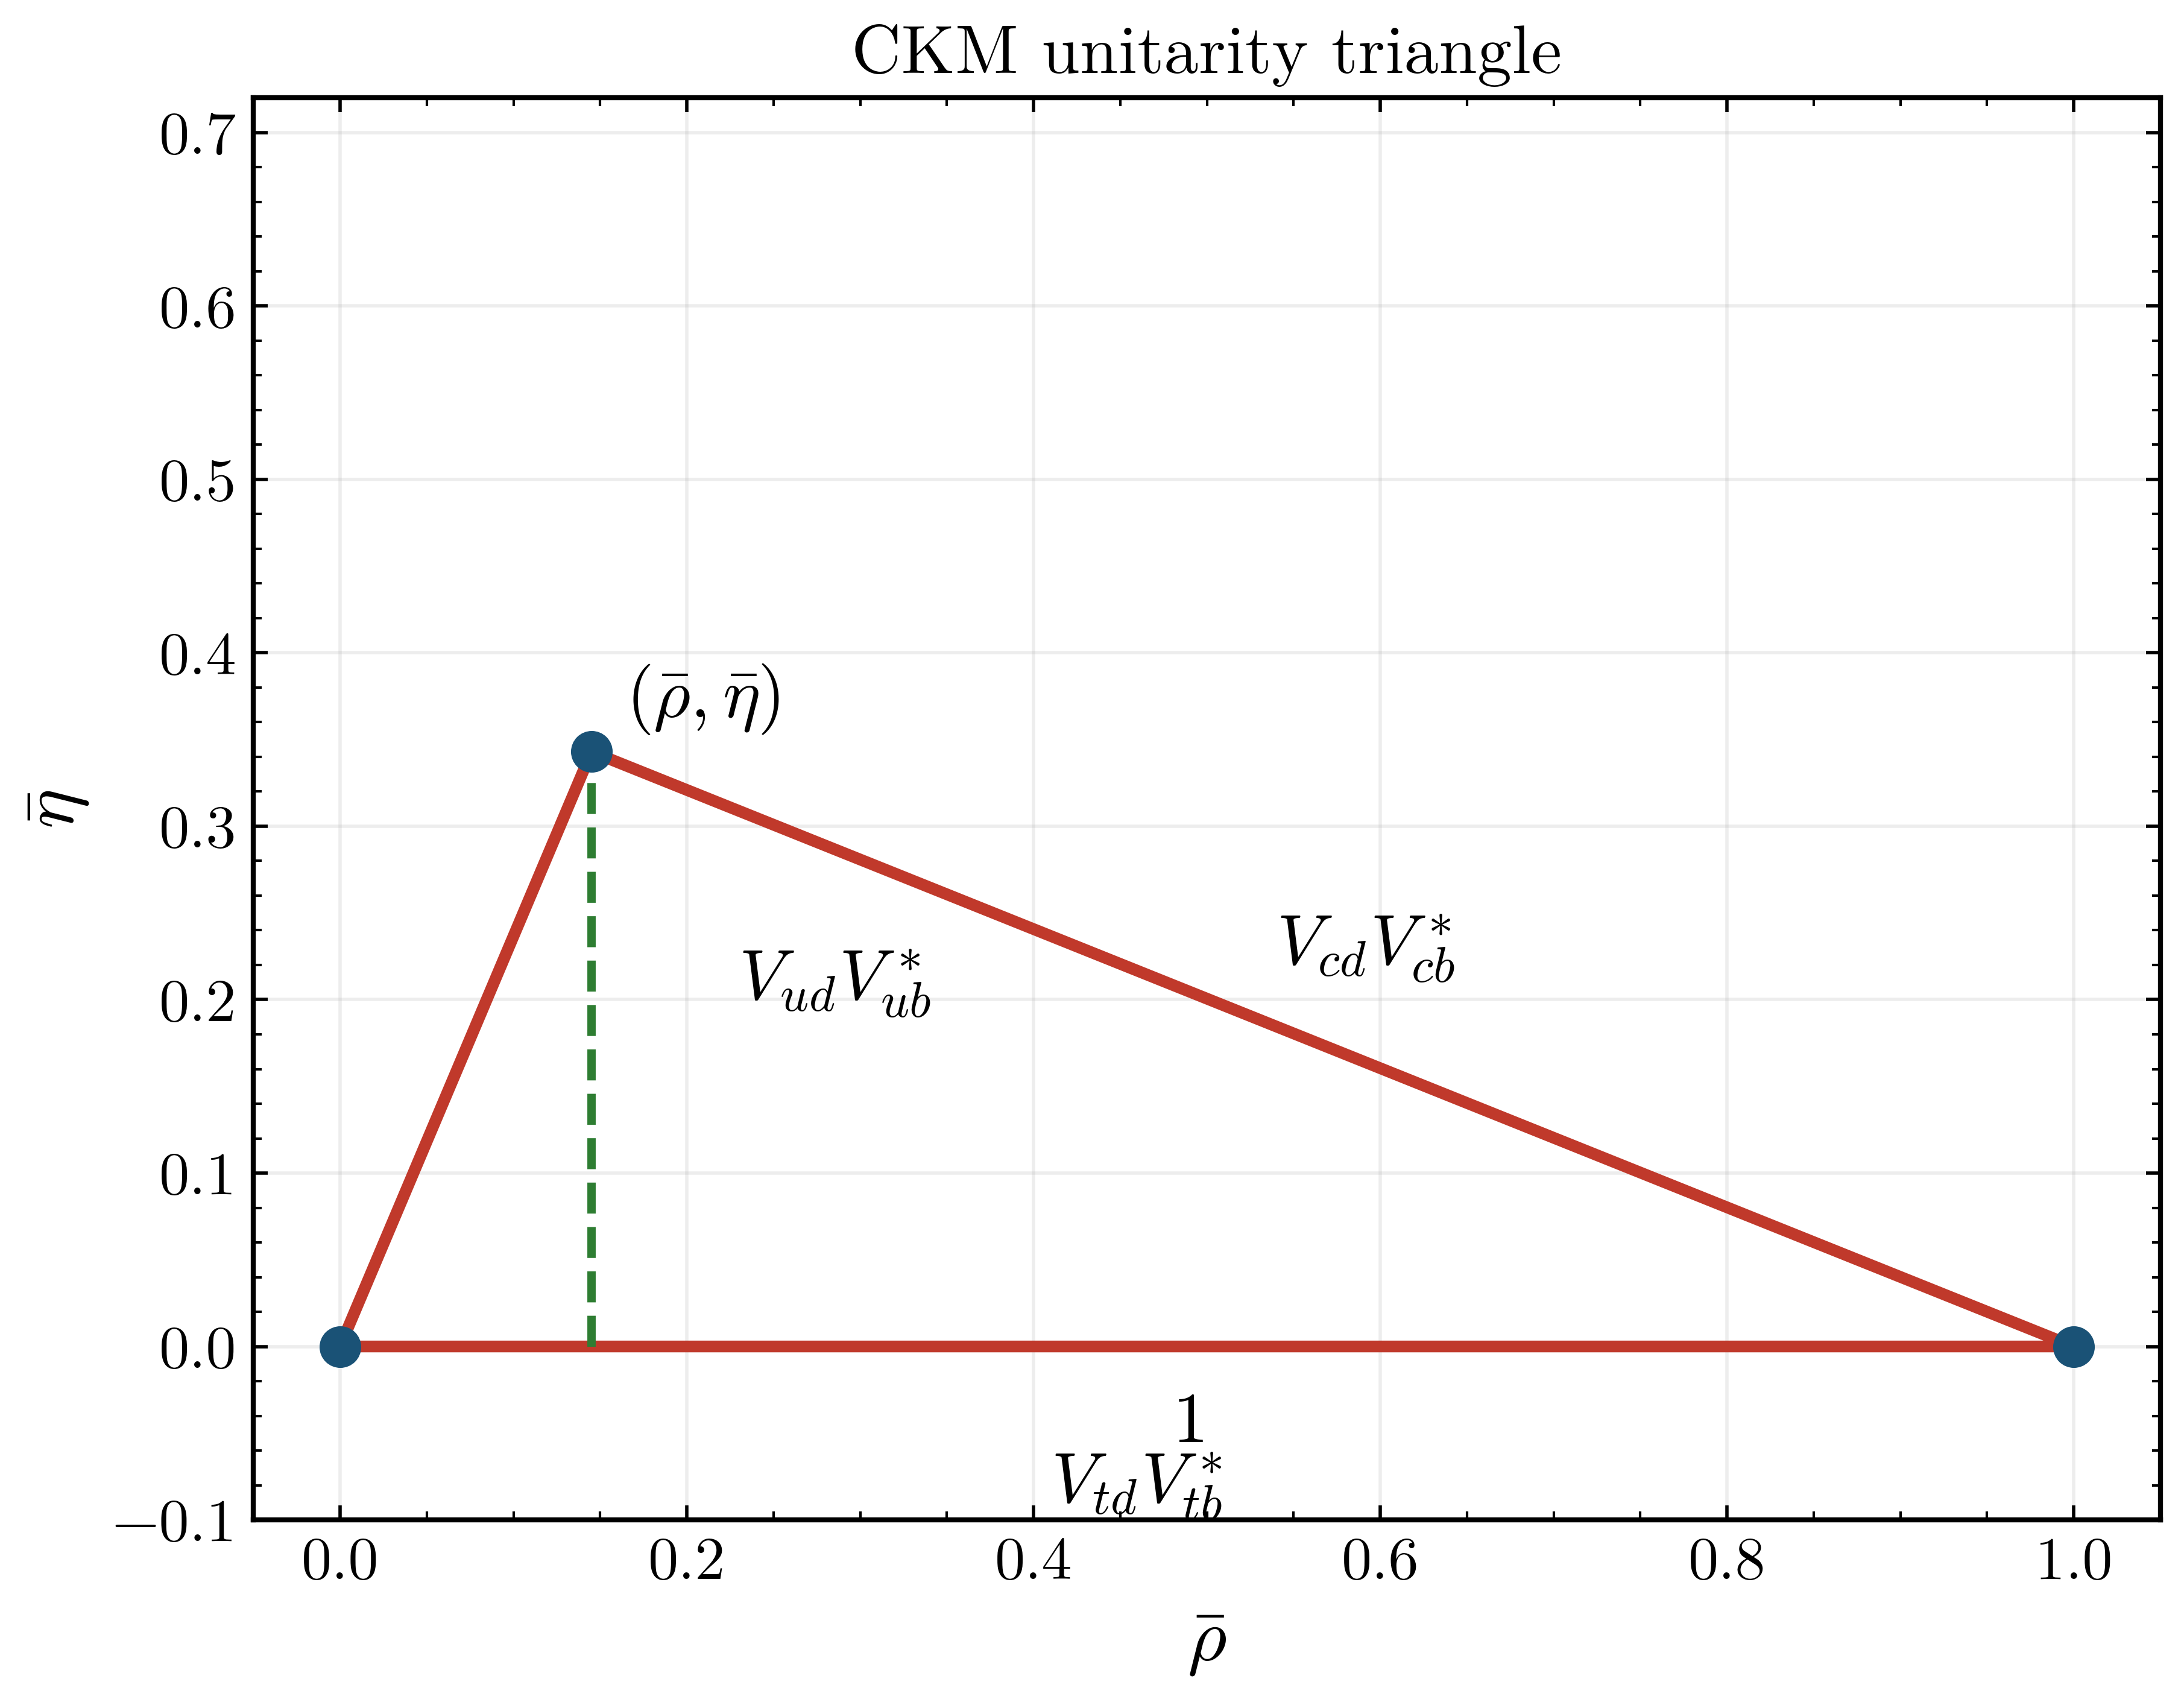
\includegraphics[width=.66\linewidth]{content/FreeElectronQuantumOptics/figures/generated/sm_ckm_unitarity_triangle_dp18.png}
\caption{CKM 幺正性不只是矩阵元素的抽象约束。以 \;\(V_{ud}V_{ub}^*+V_{cd}V_{cb}^*+V_{td}V_{tb}^*=0\) 为例，可把三项画成复平面中的闭合三角形；其非零面积正比于 Jarlskog 不变量；在上下型夸克质量谱均非简并时，它可直接编码夸克扇区的 $CP$ 破坏。图中的顶点取代表性参数点，只用于说明几何结构。}
\label{fig:sm-ckm-unitarity-triangle-dp18}
\end{figure}



最小场内容 \eqnrefs{eq:sm-one-generation-reps-dp11} 不含 $\nu_R$，也不存在维数四的可重整化中微子 Yukawa 项，所以中微子在严格最小可重整化标准模型中无质量，因此也不存在由不同中微子质量本征态相位差产生的真空振荡。现实中的中微子振荡要求扩展场论。只使用标准模型轻场时，最低维的轻子数破坏规范单态是维数五 Weinberg 算符 $(L^T C L)\Phi\Phi/\Lambda$ 的规范收缩；电弱对称性破缺把它转化为 Majorana 中微子质量矩阵，质量基与弱味基的失配由 PMNS 矩阵描述。


% 参数计数已在正文由 $2N_g-1$ 个可消去重相位一行完成；不另设推导框。

\begin{derivation}[从\eqnrefs{eq:ckm-rephasing-dp68}到\eqnrefs{eq:jarlskog-dp11}]
质量本征场仍允许保持质量项不变的矢量式重相位

\begin{equation*}
 u_i\to \ee^{\ii\alpha_i}u_i,
 \qquad
 d_j\to \ee^{\ii\beta_j}d_j.
\end{equation*}
带电流中的 CKM 元素因此变换为
\begin{equation*}
 V_{ij}\to
 \ee^{-\ii\alpha_i}V_{ij}\ee^{\ii\beta_j}.
\end{equation*}
考虑四元积
\begin{equation*}
 X_{ik;jl}\equiv V_{ij}V_{kl}V_{il}^*V_{kj}^*,
 \qquad i\neq k,
 \quad j\neq l.
\end{equation*}
四个因子分别携带相位
\begin{align*}
 V_{ij}:&\quad \ee^{-\ii\alpha_i}\ee^{+\ii\beta_j},\\
 V_{kl}:&\quad \ee^{-\ii\alpha_k}\ee^{+\ii\beta_l},\\
 V_{il}^*:&\quad \ee^{+\ii\alpha_i}\ee^{-\ii\beta_l},\\
 V_{kj}^*:&\quad \ee^{+\ii\alpha_k}\ee^{-\ii\beta_j}.
\end{align*}
相乘后 $\alpha_i,\alpha_k,\beta_j,\beta_l$ 各出现一次正号和一次负号，总相位严格等于 $1$。因此 $X_{ik;jl}$ 以及它的虚部都不依赖质量本征场的重相位选择；单个 CKM 元素的相位则没有这种性质。

取标准三角参数化 $V=R_{23}U_{13}(\delta)R_{12}$。计算\eqnrefs{eq:jarlskog-dp11} 可选择
\begin{equation*}
 J_{\rm CKM}
 =\Im\left(V_{ud}V_{cs}V_{us}^*V_{cd}^*\right).
\end{equation*}
所需四个矩阵元为
\begin{align*}
 V_{ud}&=c_{12}c_{13},\\
 V_{us}&=s_{12}c_{13},\\
 V_{cd}&=-s_{12}c_{23}-c_{12}s_{23}s_{13}\ee^{\ii\delta},\\
 V_{cs}&=c_{12}c_{23}-s_{12}s_{23}s_{13}\ee^{\ii\delta}.
\end{align*}
前两个矩阵元为实数，因此
\begin{align*}
 J_{\rm CKM}
 =c_{12}s_{12}c_{13}^2\,
 \Im\Big[&
 (c_{12}c_{23}-s_{12}s_{23}s_{13}\ee^{\ii\delta})\\
 &\times(-s_{12}c_{23}-c_{12}s_{23}s_{13}\ee^{-\ii\delta})
 \Big].
\end{align*}
把括号展开：
\begin{align*}
 {}&-c_{12}s_{12}c_{23}^2
 -c_{12}^2c_{23}s_{23}s_{13}\ee^{-\ii\delta}\\
 &\qquad
 +s_{12}^2c_{23}s_{23}s_{13}\ee^{\ii\delta}
 +c_{12}s_{12}s_{23}^2s_{13}^2.
\end{align*}
第一项和最后一项为实数；中间两项的虚部为
\begin{align*}
 &c_{12}^2c_{23}s_{23}s_{13}\sin\delta
 +s_{12}^2c_{23}s_{23}s_{13}\sin\delta\\
 &=(c_{12}^2+s_{12}^2)c_{23}s_{23}s_{13}\sin\delta\\
 &=c_{23}s_{23}s_{13}\sin\delta.
\end{align*}
所以
\begin{equation*}
 J_{\rm CKM}
 =c_{12}c_{23}c_{13}^2s_{12}s_{23}s_{13}\sin\delta,
\end{equation*}
即\eqnrefs{eq:jarlskog-dp11}。

三代幺正性进一步固定所有异行异列四元积的相对符号。定义
\begin{equation*}
 \mathcal J_{ij;\alpha\beta}
 \equiv\Im\!\left(
 V_{i\alpha}V_{j\beta}V_{i\beta}^*V_{j\alpha}^*
 \right),
 \qquad i\neq j,\quad \alpha\neq\beta.
\end{equation*}
交换两行或两列都会把括号内的复数变为其复共轭，因此
\begin{equation*}
 \mathcal J_{ji;\alpha\beta}
 =-\mathcal J_{ij;\alpha\beta},
 \qquad
 \mathcal J_{ij;\beta\alpha}
 =-\mathcal J_{ij;\alpha\beta}.
\end{equation*}
再固定一对不同的行 $i,j$ 与一列 $\alpha$。行正交性给
\begin{equation*}
 \sum_{\lambda=1}^{3}V_{i\lambda}V_{j\lambda}^*=0.
\end{equation*}
乘以 $V_{i\alpha}^*V_{j\alpha}$ 并取虚部，$\lambda=\alpha$ 项为实数，于是其余两列 $\beta,\gamma$ 满足
\begin{equation*}
 \mathcal J_{ij;\beta\alpha}
 +\mathcal J_{ij;\gamma\alpha}=0.
\end{equation*}
结合列交换的反对称性，固定行对时三个不同列对的四元积虚部具有相同绝对值，并按列指标的奇偶排列改变符号。

为了比较不同的行对，固定两列 $\alpha\neq\beta$ 与一行 $i$。列正交性给
\begin{equation*}
 \sum_{r=1}^{3}V_{r\alpha}V_{r\beta}^*=0.
\end{equation*}
乘以 $V_{i\alpha}^*V_{i\beta}$ 并取虚部，$r=i$ 项为
$|V_{i\alpha}|^2|V_{i\beta}|^2$，其虚部为零，因此剩余两行 $j,k$ 满足
\begin{equation*}
 \Im\!\left(
 V_{j\alpha}V_{j\beta}^*
 V_{i\alpha}^*V_{i\beta}
 \right)
 +
 \Im\!\left(
 V_{k\alpha}V_{k\beta}^*
 V_{i\alpha}^*V_{i\beta}
 \right)=0.
\end{equation*}
把每一项重新排列成 $\mathcal J$ 的定义，并使用行交换的反对称性，就得到固定列对时不同的行对具有相同绝对值，并按行指标排列改变符号。以
\begin{equation*}
 \mathcal J_{12;12}
 =\Im(V_{ud}V_{cs}V_{us}^*V_{cd}^*)
 \equiv J_{\rm CKM}
\end{equation*}
固定总体符号，便得到三代幺正矩阵的恒等式
\begin{equation*}
 \mathcal J_{ij;\alpha\beta}
 =J_{\rm CKM}\,\epsilon_{ijk}\epsilon_{\alpha\beta\gamma},
\end{equation*}
其中 $k$ 与 $\gamma$ 分别是剩余的第三个行、列指标。这就是三代幺正矩阵的一般四元积恒等式。

\end{derivation}

\begin{derivation}[从\eqnrefs{eq:jarlskog-dp11}到\eqnrefs{eq:jarlskog-determinant-dp11}]
定义两个厄米矩阵

\begin{equation*}
 H_u\equiv Y_uY_u^\dagger,
 \qquad
 H_d\equiv Y_dY_d^\dagger.
\end{equation*}
在共同左手弱基变换 $Q_L\to U_QQ_L$ 下，
\begin{equation*}
 H_u\to U_QH_uU_Q^\dagger,
 \qquad
 H_d\to U_QH_dU_Q^\dagger.
\end{equation*}
因此对易子
\begin{equation*}
 C\equiv[H_u,H_d]
\end{equation*}
只作相似变换 $C\to U_QCU_Q^\dagger$，所以 $\det C$ 与弱基选择无关。又因为 $H_u,H_d$ 厄米，
\begin{equation*}
 C^\dagger=-C,
\end{equation*}
三代时 $\det C$ 必为纯虚数。

选择上型夸克质量基，并简记
\begin{equation*}
 a_i\equiv y_{u_i}^2,
 \qquad
 b_\alpha\equiv y_{d_\alpha}^2.
\end{equation*}
于是
\begin{equation*}
 H_u=\operatorname{diag}(a_1,a_2,a_3),
 \qquad
 H_d=V\operatorname{diag}(b_1,b_2,b_3)V^\dagger,
\end{equation*}
其中 $V=V_{\rm CKM}$。对易子的矩阵元为
\begin{align*}
 C_{ij}
 &=(a_i-a_j)(H_d)_{ij},\\
 (H_d)_{ij}
 &=\sum_{\alpha=1}^{3}V_{i\alpha}b_\alpha V_{j\alpha}^*.
\end{align*}
特别地 $C_{ii}=0$。因此三阶行列式只剩两个三循环项：
\begin{equation*}
 \det C=C_{12}C_{23}C_{31}+C_{13}C_{21}C_{32}.
\end{equation*}
定义
\begin{equation*}
 \Delta_u\equiv
 (a_1-a_2)(a_1-a_3)(a_2-a_3).
\end{equation*}
第一个循环的上型谱因子为
\begin{align*}
 &(a_1-a_2)(a_2-a_3)(a_3-a_1)\\
 &=-\Delta_u,
\end{align*}
第二个循环的上型谱因子为
\begin{align*}
 &(a_1-a_3)(a_2-a_1)(a_3-a_2)\\
 &=+\Delta_u.
\end{align*}
又因为 $H_d$ 厄米，令
\begin{equation*}
 z\equiv(H_d)_{12}(H_d)_{23}(H_d)_{31},
\end{equation*}
则
\begin{equation*}
 (H_d)_{13}(H_d)_{21}(H_d)_{32}=z^*.
\end{equation*}
所以
\begin{align*}
 \det C
 &=\Delta_u(z^*-z)\\
 &=-2\ii\Delta_u\Im z.
\end{align*}
问题于是化为计算 $\Im z$。

由于单位矩阵的非对角元为零，给 $H_d$ 加上任意常数倍单位矩阵都不改变 $z$。因此可以从所有 $b_\alpha$ 中减去 $b_3$，定义
\begin{equation*}
 x\equiv b_1-b_3,
 \qquad
 y\equiv b_2-b_3.
\end{equation*}
对 $i\neq j$，
\begin{equation*}
 (H_d)_{ij}
 =xV_{i1}V_{j1}^*+yV_{i2}V_{j2}^*.
\end{equation*}
于是 $z$ 是 $x,y$ 的三次齐次多项式。纯 $x^3$ 项为
\begin{equation*}
 x^3|V_{11}V_{21}V_{31}|^2,
\end{equation*}
纯 $y^3$ 项为
\begin{equation*}
 y^3|V_{12}V_{22}V_{32}|^2,
\end{equation*}
二者都为实数，不贡献 $\Im z$。

$x^2y$ 的三个交叉项的虚部分别是
\begin{align*}
 \Im\!\big[(V_{11}V_{21}^*)(V_{21}V_{31}^*)(V_{32}V_{12}^*)\big]
 &=-J_{\rm CKM}|V_{21}|^2,\\
 \Im\!\big[(V_{11}V_{21}^*)(V_{22}V_{32}^*)(V_{31}V_{11}^*)\big]
 &=-J_{\rm CKM}|V_{11}|^2,\\
 \Im\!\big[(V_{12}V_{22}^*)(V_{21}V_{31}^*)(V_{31}V_{11}^*)\big]
 &=-J_{\rm CKM}|V_{31}|^2.
\end{align*}
三代幺正矩阵的四元积满足
\begin{equation*}
 \Im(V_{i\alpha}V_{j\beta}V_{i\beta}^*V_{j\alpha}^*)
 =J_{\rm CKM}\,\epsilon_{ijk}\epsilon_{\alpha\beta\gamma},
\end{equation*}
其中未写出的 $k,\gamma$ 是各自剩余的第三个指标。由第一列归一化
\begin{equation*}
 |V_{11}|^2+|V_{21}|^2+|V_{31}|^2=1,
\end{equation*}
故全部 $x^2y$ 项的虚部为
\begin{equation*}
 -J_{\rm CKM}x^2y.
\end{equation*}
对 $xy^2$ 项逐个应用四元积恒等式，三个虚部分别是
\begin{align*}
 \Im(V_{11}V_{22}V_{12}^*V_{21}^*)|V_{32}|^2
 &=+J_{\rm CKM}|V_{32}|^2,\\
 \Im(V_{21}V_{32}V_{22}^*V_{31}^*)|V_{12}|^2
 &=+J_{\rm CKM}|V_{12}|^2,\\
 \Im(V_{31}V_{12}V_{32}^*V_{11}^*)|V_{22}|^2
 &=+J_{\rm CKM}|V_{22}|^2.
\end{align*}
三项相加后利用第二列归一化得到
\begin{equation*}
 +J_{\rm CKM}xy^2.
\end{equation*}
因此
\begin{align*}
 \Im z
 &=J_{\rm CKM}xy(y-x)\\
 &=-J_{\rm CKM}(b_1-b_2)(b_1-b_3)(b_2-b_3)\\
 &=-J_{\rm CKM}\Delta_d.
\end{align*}
代回 $\det C=-2\ii\Delta_u\Im z$：
\begin{equation*}
 \det[H_u,H_d]
 =2\ii J_{\rm CKM}\Delta_u\Delta_d,
\end{equation*}
即\eqnrefs{eq:jarlskog-determinant-dp11}。

这个推导还直接给出两个退化检查：若任意两种上型 Yukawa 本征值相同，则 $\Delta_u=0$；若任意两种下型本征值相同，则 $\Delta_d=0$。任一情形都使所有弱基不变的 $CP$ 奇量消失，因为相应简并子空间内出现额外的味旋转自由度。
\end{derivation}


% 幺正三角形面积由复平面二维行列式一行得到，正文已给出结果；不另设推导框。


\subsection{GIM 抵消与环级味改变中性流}\label{subsec:sm-gim-dp83}

质量本征基中的光子、胶子和 $Z$ 中性流都与味指标成正比于单位矩阵，因此树级中性流不会把一个下型夸克质量本征态变成另一个。两个带电弱顶角却可以在圈内先把外部 $d_j$ 变成上型夸克 $u_i$，再变回 $d_k$；味改变中性流因此第一次在圈级出现。每个单独圈图一般依赖规范和中间参数化，只有把给定过程在该阶所需的规范不变图集合相加以后，才能把内部质量依赖压缩成物理圈函数。

对一般 $d_j\to d_k$（$j\ne k$）的一圈味改变中性流，先选取一组完备、线性无关的外部 Lorentz--Dirac 算符结构 $\mathcal K_a(p_{\rm ext})$。把给定微扰阶所需的顶角图、自能图、Goldstone 与鬼场图按规范不变组合求和后，振幅可唯一分解为
\begin{equation}
 \boxed{
 \mathcal A_{j\to k}^{\rm FCNC}
 =\sum_a \mathcal K_a(p_{\rm ext})\,C_a^{jk},
 \qquad
 C_a^{jk}
 =\sum_iV_{ik}^*V_{ij}F_a(x_i),}
 \label{eq:sm-gim-loop-sum-dp83}
\end{equation}
其中
\begin{equation*}
 x_i\equiv\frac{m_{u_i}^2}{m_W^2},
 \qquad u_i\in\{u,c,t\}.
\end{equation*}
$F_a(x_i)$ 是第 $a$ 个独立算符系数在内部上型夸克质量为 $m_{u_i}$ 时的完整一圈函数；所有与内部味无关的规范耦合、外部运动学与归一化因子都已按同一方式包含在 $\mathcal K_a$ 或 $F_a$ 的定义中。两个带电流顶角分别给出 $V_{ij}$ 与 $V_{ik}^*$，因此内部味只通过 $V_{ik}^*V_{ij}$ 与 $x_i$ 进入。

CKM 幺正性给出非对角关系
\begin{equation}
 \boxed{
 \sum_iV_{ik}^*V_{ij}=(V^\dagger V)_{kj}=0,
 \qquad j\ne k.}
 \label{eq:sm-gim-unitarity-dp83}
\end{equation}
于是对每一个独立算符系数、对任意参考点 $x_*$ 都有恒等式
\begin{equation}
 \boxed{
 C_a^{jk}
 =\sum_iV_{ik}^*V_{ij}\,[F_a(x_i)-F_a(x_*)],
 \qquad j\ne k.}
 \label{eq:sm-gim-subtracted-exact-dp85}
\end{equation}
若所有内部上型夸克质量简并，则所有 $x_i$ 相同，右端逐项差值相同并被\eqnrefs{eq:sm-gim-unitarity-dp83} 消去，因此每个 $C_a^{jk}$ 都为零。这就是 GIM 机制与具体过程无关的代数核心。

只有在所考察的 $F_a(x)$ 在 $x=0$ 邻域至少二次可微、并且参与展开的全部 $x_i\ll1$ 时，才把\eqnrefs{eq:sm-gim-subtracted-exact-dp85} 进一步展开。取 $x_*=0$，Taylor 定理给
\begin{equation}
 \boxed{
 C_a^{jk}
 =F_a'(0)
 \sum_iV_{ik}^*V_{ij}\frac{m_{u_i}^2}{m_W^2}
 +\mathcal R_{a,jk}^{(\ge2)},}
 \label{eq:sm-gim-mass-suppression-dp83}
\end{equation}
其中 $\mathcal R_{a,jk}^{(\ge2)}$ 从 $x_i^2$ 阶开始，节末推导给出显式余项界。若具体圈函数含 $x\ln x$ 等非解析小质量项，或顶夸克满足 $x_t=O(1)$，则直接使用\eqnrefs{eq:sm-gim-subtracted-exact-dp85} 的精确差值，不使用局域 Taylor 形式。

\begin{derivation}[从\eqnrefs{eq:sm-gim-loop-sum-dp83}到\eqnrefs{eq:sm-gim-mass-suppression-dp83}]
质量本征基中的夸克带电流为
\begin{equation*}
 \Lag_{\rm CC}^{q}
 =-\frac{\hbar c\,g}{\sqrt2}
 \left[
 \bar u_i\gamma^\mu P_LV_{ij}d_j\,\mathcal W_\mu^+
 +\bar d_j\gamma^\mu P_LV_{ij}^*u_i\,\mathcal W_\mu^-
 \right].
\end{equation*}
考虑 $d_j\to d_k$、$j\neq k$ 的一圈味改变中性流。Dyson 展开中任意包含两个带电流顶角的收缩，都含味因子
\begin{equation*}
 V_{ij}V_{ik}^*=V_{ik}^*V_{ij},
\end{equation*}
因为第一个顶角把外部 $d_j$ 连接到内部 $u_i$，第二个厄米共轭顶角再把同一内部味 $u_i$ 连接到外部 $d_k$。

给定外部粒子与动量后，选一组完备、线性无关的 Lorentz--Dirac 算符基 $\{\mathcal K_a(p_{\rm ext})\}$。同一微扰阶的全部规范完成图求和后，任意内部味 $i$ 的贡献都能按这组基展开：
\begin{equation*}
 \mathcal A_{j\to k}^{(i)}
 =V_{ik}^*V_{ij}
 \sum_a\mathcal K_a(p_{\rm ext})F_a(x_i),
 \qquad
 x_i=\frac{m_{u_i}^2}{m_W^2}.
\end{equation*}
这里 $F_a$ 由实际圈积分定义。例如在维数正规化中，每个 $F_a$ 都来自形如
\begin{equation*}
 \mu_{\rm DR}^{2\epsilon}
 \int\frac{\dd^d\ell}{(2\pi)^d}
 \frac{N_a(\ell,p_{\rm ext};m_{u_i},m_W)}
 {\prod_r D_r(\ell,p_{\rm ext};m_{u_i},m_W)}
\end{equation*}
的积分及同阶规范完成项。对内部味求和并交换有限求和与算符基展开，得到
\begin{align*}
 \mathcal A_{j\to k}^{\rm FCNC}
 &=\sum_i\mathcal A_{j\to k}^{(i)}\\
 &=\sum_a\mathcal K_a(p_{\rm ext})
 \left[\sum_iV_{ik}^*V_{ij}F_a(x_i)\right].
\end{align*}
因此
\begin{equation*}
 C_a^{jk}=\sum_iV_{ik}^*V_{ij}F_a(x_i),
\end{equation*}
即正文\eqnrefs{eq:sm-gim-loop-sum-dp83}。

CKM 幺正性 $V^\dagger V=I$ 的非对角元满足
\begin{equation*}
 \sum_iV_{ik}^*V_{ij}=0,
 \qquad j\neq k.
\end{equation*}
对任意参考点 $x_*$，逐个算符系数加减同一个 $F_a(x_*)$：
\begin{align*}
 C_a^{jk}
 &=\sum_iV_{ik}^*V_{ij}
 \left[F_a(x_i)-F_a(x_*)+F_a(x_*)\right]\\
 &=\sum_iV_{ik}^*V_{ij}[F_a(x_i)-F_a(x_*)]
 +F_a(x_*)\sum_iV_{ik}^*V_{ij}\\
 &=\sum_iV_{ik}^*V_{ij}[F_a(x_i)-F_a(x_*)].
\end{align*}
这就是\eqnrefs{eq:sm-gim-subtracted-exact-dp85}。若 $x_i=x_*$ 对所有内部味都成立，则每个独立算符系数 $C_a^{jk}$ 都等于零，因而完整振幅为零。

若 $F_a$ 在连接 $x_*$ 与 $x_i$ 的区间可微，微积分基本定理还给出精确质量差表示
\begin{align*}
 F_a(x_i)-F_a(x_*)
 &=\int_{x_*}^{x_i}\dd y\,F_a'(y)\\
 &=(x_i-x_*)\int_0^1\dd t\,
 F_a'\!\left[x_*+t(x_i-x_*)\right],
\end{align*}
因此
\begin{equation*}
 C_a^{jk}
 =\sum_iV_{ik}^*V_{ij}(x_i-x_*)
 \int_0^1\dd t\,
 F_a'\!\left[x_*+t(x_i-x_*)\right].
\end{equation*}
这条等式直接表明共同的内部质量部分被消去，剩余量由质量劈裂加权。

对轻内部质量取 $x_*=0$。若 $F_a\in C^3([0,x_{\max}])$，Taylor 定理带积分余项给
\begin{equation*}
 F_a(x_i)
 =F_a(0)+x_iF_a'(0)+\frac{x_i^2}{2}F_a''(0)
 +\frac{x_i^3}{2}\int_0^1\dd t\,(1-t)^2F_a^{(3)}(tx_i).
\end{equation*}
代入并使用 $\sum_iV_{ik}^*V_{ij}=0$：
\begin{equation*}
 C_a^{jk}
 =F_a'(0)\sum_iV_{ik}^*V_{ij}x_i
 +\mathcal R_{a,jk}^{(\ge2)},
\end{equation*}
其中
\begin{align*}
 \mathcal R_{a,jk}^{(\ge2)}
 &\equiv
 \frac{F_a''(0)}2
 \sum_iV_{ik}^*V_{ij}x_i^2+R_{a,jk}^{(3)},\\
 R_{a,jk}^{(3)}
 &\equiv
 \frac12\sum_iV_{ik}^*V_{ij}x_i^3
 \int_0^1\dd t\,(1-t)^2F_a^{(3)}(tx_i).
\end{align*}
于是
\begin{align*}
 |R_{a,jk}^{(3)}|
 &\le\frac16
 \max_{0\le y\le x_{\max}}|F_a^{(3)}(y)|
 \sum_i|V_{ik}^*V_{ij}|x_i^3,\\
 |\mathcal R_{a,jk}^{(\ge2)}|
 &\le\frac{|F_a''(0)|}{2}
 \sum_i|V_{ik}^*V_{ij}|x_i^2
 +|R_{a,jk}^{(3)}|.
\end{align*}
最后用 $x_i=m_{u_i}^2/m_W^2$ 即得到正文\eqnrefs{eq:sm-gim-mass-suppression-dp83} 及其余项控制。若 $F_a$ 在零点附近非解析，或某个 $x_i$ 不小，则保留精确差值\eqnrefs{eq:sm-gim-subtracted-exact-dp85}。
\end{derivation}


\subsection{量子规范一致性、全局流与拓扑}\label{subsec:sm-gauge-anomaly-cancellation-dp32}

经典作用量把同一规范轨道上的场配置识别为同一物理态。量子化后的物理态空间必须保持这种规范等价：若圈修正让规范等价的场配置得到不同的量子振幅，纵向的非物理自由度就不能再从可观测振幅中一致消去，理论本身会失去幺正的物理态解释。手征费米子恰好会带来这种风险，因为定义费米子路径积分测度时所需的紫外正则化可能产生一个非平凡 Jacobian。这个由量子测度破坏经典规范冗余的现象称为规范反常。

是否发生这种破坏，可以直接由三角图中的群表示因子判断。对三个非阿贝尔规范流，其系数由对称迹
\begin{equation*}
 d_R^{abc}=2\Tr_R\!\left[T^a\{T^b,T^c\}\right]
\end{equation*}
控制。若被破坏的是局域规范流，这个系数必须在完整的左手 Weyl 费米子谱上精确相消，而不能把反常解释成可接受的量子修正。

对一般左手 Weyl 场 $f$，若其表示为 $R_{3f}\otimes R_{2f}$、超荷为 $Y_f$，先把三个群论数字定义清楚。$d_a(R)$ 是表示空间维数；Dynkin 指标 $T_a(R)$ 由
\begin{equation*}
 \Tr_R(T^AT^B)=T_a(R)\delta^{AB}
\end{equation*}
定义，因而控制两个非阿贝尔生成元进入三角图时的迹；$SU(3)$ 三次反常指标 $A_3(R)$ 则由对称三生成元迹相对于基本表示的系数定义，共轭表示满足 $A_3(\bar R)=-A_3(R)$。因此，混合反常使用 $T_a(R)$，纯 $SU(3)^3$ 反常使用对三生成元共轭敏感的 $A_3(R)$。四维标准模型相关的局域规范反常系数可统一写成
\begin{equation}
\boxed{
\begin{aligned}
C_{333}&=\sum_f d_2(R_{2f})A_3(R_{3f}),\\
C_{33Y}&=\sum_f d_2(R_{2f})Y_fT_3(R_{3f}),\\
C_{22Y}&=\sum_f d_3(R_{3f})Y_fT_2(R_{2f}),\\
C_{YYY}&=\sum_f d_3(R_{3f})d_2(R_{2f})Y_f^3,\\
C_{{\rm grav}^2Y}&=\sum_f d_3(R_{3f})d_2(R_{2f})Y_f.
\end{aligned}}
\label{eq:general-chiral-anomaly-coefficients-dp75}
\end{equation}
局域量子规范一致性要求这些系数全部为零。$SU(2)$ 的有限维表示为实或伪实，因此没有独立的局域 $SU(2)^3$ 三次反常；但局域三角图并未穷尽全局拓扑障碍。

统一采用左手 Weyl 场记账最为直接。右手场 $\psi_R$ 改写为左手荷共轭场 $\psi_R^c$ 后，非阿贝尔表示变为共轭表示，$U(1)$ 荷变号。标准模型每一代的左手场谱为
\begin{align}
 Q_L&:(\mathbf3,\mathbf2,+\tfrac16),&
 u_R^c&:(\bar{\mathbf3},\mathbf1,-\tfrac23),\\
 d_R^c&:(\bar{\mathbf3},\mathbf1,+\tfrac13),&
 L_L&:(\mathbf1,\mathbf2,-\tfrac12),\\
 e_R^c&:(\mathbf1,\mathbf1,+1).
 \label{eq:sm-left-weyl-anomaly-set-dp11}
\end{align}
这里三元组依次表示 $SU(3)_c$、$SU(2)_L$ 表示与超荷 $Y$。这一场谱必须同时满足
\begin{equation}
 \boxed{
 C_{333}^{\rm anom}=
 C_{33Y}^{\rm anom}=
 C_{22Y}^{\rm anom}=
 C_{YYY}^{\rm anom}=
 C_{{\rm grav}^2Y}^{\rm anom}=0.}
 \label{eq:sm-gauge-anomaly-cancellation-dp32}
\end{equation}
此外，纯 $[SU(3)_c]^3$ 反常也必须抵消。$SU(2)$ 基本表示是伪实表示，因此局部三角图不会产生 $SU(2)^3$ 反常，但局部微扰展开并未检查规范变换空间的全局拓扑。把欧几里得四维时空在无穷远固定后紧化为 $S^4$，一个大规范变换可看成连续映射 $U:S^4\to SU(2)$。记号 $\pi_4(SU(2))$ 表示这类映射在连续变形下的同伦分类；$\pi_4(SU(2))=\mathbb Z_2$ 意味着只有平凡类与一个不能连续缩回恒等变换的非平凡类。Witten 的全局反常定理指出：沿这个非平凡类作规范变换时，单个左手 $SU(2)$ 基本二重态的费米子泛函积分整体变号。因此含 $N_D$ 个基本左手二重态时总符号为 $(-1)^{N_D}$，量子规范不变性要求 $N_D$ 为偶数。标准模型每一代含三个颜色副本的 $Q_L$ 与一个 $L_L$，故 $N_D=4$，模二全局障碍消失。

规范不变的 Yukawa 耦合还把左、右手超荷彼此联系。若暂以
\begin{equation*}
 Y_Q=q,\quad Y_u=u,\quad Y_d=d,\quad
 Y_L=\ell,\quad Y_e=e,\quad Y_\Phi=h
\end{equation*}
表示一代超荷，则三条 Yukawa 单态条件与两个独立的线性反常条件可整理成
\begin{equation}
\boxed{
 u=q+h,\qquad d=q-h,\qquad e=\ell-h,\qquad
 3q+\ell=0,\qquad
 6q-3u-3d+2\ell-e=0.}
\label{eq:sm-hypercharge-constraint-system-dp68}
\end{equation}
这组方程把相对超荷固定到一个整体归一化。取 Higgs 约定 $h=1/2$ 后得到
\begin{equation}
 \boxed{
 Y_Q=\frac16,\quad Y_u=\frac23,\quad Y_d=-\frac13,\quad
 Y_L=-\frac12,\quad Y_e=-1,\quad Y_\Phi=\frac12.}
 \label{eq:sm-hypercharge-solution-dp32}
\end{equation}
因此标准模型超荷并不是只为重现实验电荷而填写的一张表；同一组数还必须允许 Yukawa 质量耦合，并同时满足局域与全局规范一致性条件。任何改变手征费米子场内容的新物理模型，都必须重新检查这些条件。

\label{subsec:sm-global-axial-anomaly-dp32}
局域规范反常的精确抵消保证量子规范理论可以一致定义；与此不同，物理全局流允许出现由量子测度产生的反常，并留下可观测的拓扑效应。

规范反常必须抵消，但全局流的反常可以成为真实的量子效应。对一个 Dirac 费米子，经典轴流
\begin{equation*}
 J_5^\mu=\bar\psi\gamma^\mu\gamma^5\psi
\end{equation*}
在有质量时已经满足 $\partial_\mu J_5^\mu=(2\ii mc/\hbar)\bar\psi\gamma^5\psi$；量子化后，费米子测度还产生规范场的拓扑密度。对单位电荷 QED 费米子，采用对偶场强的定义后，结果为
\begin{equation}
 \boxed{
 \partial_\mu J_5^\mu
 =\frac{2\ii mc}{\hbar}\bar\psi\gamma^5\psi
 +\frac{g_{\rm em}^2}{8\pi^2}
 F_{\mu\nu}^{\rm geo}{}^\star\!F_{\rm geo}^{\mu\nu}
 =\frac{2\ii mc}{\hbar}\bar\psi\gamma^5\psi
 +\frac{e^2}{8\pi^2\hbar^2}
 F_{\mu\nu}{}^\star\!F^{\mu\nu}.}
 \label{eq:abj-anomaly-qed-dp11}
\end{equation}
第二个等号使用 \eqnrefs{eq:sm-photon-geo-si-bridge-dp75}，其中末项的 $F_{\mu\nu}$ 是前面 QED 章节固定的 SI 电磁场强。这里异常的是全局轴对称性，而不是电磁 $U(1)$ 规范对称性；矢量规范流仍必须保持守恒。

在路径积分量子化中，费米子场不是对每个时空点上的普通数值直接积分，而是先在一组完备正交的单粒子函数 $\{\phi_n(x)\}$ 上展开。若
\begin{equation*}
 q(x)=\sum_n a_n\phi_n(x),
 \qquad
 \bar q(x)=\sum_n\bar b_n\phi_n^\dagger(x),
\end{equation*}
则 $a_n,\bar b_n$ 是反交换的 Grassmann 系数。所谓\emph{费米子路径积分测度}，就是对全部这些系数作 Berezin 积分的乘积
\begin{equation*}
 \mathcal Dq\,\mathcal D\bar q
 \equiv\prod_n\dd a_n\,\dd\bar b_n.
\end{equation*}
场的局域线性变换会同时线性变换无穷多个系数，因此测度一般获得一个 Jacobian。Fujikawa 方法的核心就是用保持规范协变性的正则化来计算这个无穷维 Jacobian；若 Jacobian 不等于一，经典作用量的对称性在量子理论中便产生反常。

对 $N_f$ 个 QCD 基本表示夸克，考虑共同的轴向旋转
\begin{equation}
\boxed{
 q_f\to \ee^{\ii\alpha\gamma^5}q_f,
 \qquad
 \bar q_f\to \bar q_f\ee^{\ii\alpha\gamma^5}.}
\label{eq:qcd-singlet-axial-rotation-dp68}
\end{equation}
经典无质量作用量在这一变换下不变，但路径积分测度的 Jacobian 不为一。因此味单态轴流 $J_5^\mu=\sum_f\bar q_f\gamma^\mu\gamma^5q_f$ 满足
\begin{equation}
 \boxed{
 \partial_\mu J_5^\mu
 =\sum_f\frac{2\ii m_fc}{\hbar}\bar q_f\gamma^5q_f
 +\frac{N_f g_s^2}{16\pi^2}
 \mathcal F_{\mu\nu}^a{}^\star\!\mathcal F^{a\mu\nu}.}
 \label{eq:qcd-singlet-axial-anomaly-dp32}
\end{equation}
所以轻夸克极限中的 $U(1)_A$ 不会像非单态 $SU(N_f)_A$ 那样产生额外的轻 Goldstone 模式；非微扰 QCD 的手征凝聚与轴反常分别控制非单态和味单态两个不同的对称性问题。

电弱 $SU(2)_L$ 的拓扑扇区还使经典重整化标准模型中的重子数 $B$ 与轻子数 $L$ 发生全局反常。拓扑荷定义为
\begin{equation}
\boxed{
 \nu=\frac{g^2}{32\pi^2}
 \int\dd^4 x\,
 \mathcal W_{\mu\nu}^I{}^\star\!\mathcal W^{I\mu\nu}
 \in\mathbb Z.}
\label{eq:electroweak-topological-charge-dp68}
\end{equation}
这里的\emph{零模}是欧几里得手征 Dirac 算符满足 $\slashed D_E\psi_0=0$ 的归一化本征函数。Atiyah--Singer 指数定理给出表示 $R$ 中左右手零模数之差
\begin{equation*}
 n_L-n_R=2T(R)\nu.
\end{equation*}
对 $SU(2)$ 基本表示 $T(\mathbf2)=1/2$，所以 $|\nu|=1$ 的拓扑背景为每个左手弱二重态提供一个不可由非零本征值配对消去的手征零模。Grassmann 路径积分只有在外场插入把这些零模全部饱和时才非零；由这些零模诱导的局域多费米子结构称为 't Hooft 顶点。每一代的三个颜色 $Q_L$ 二重态和一个 $L_L$ 二重态因而共同给出一组 $QQQL$ 型插入。对一般世代数 $N_g$，相应选择定则为
\begin{equation}
 \boxed{
 \Delta B=\Delta L=N_g\nu,\qquad
 \Delta(B-L)=0,\qquad
 \Delta(B+L)=2N_g\nu.}
 \label{eq:sm-bplusl-selection-dp32}
\end{equation}
这与规范反常抵消并不矛盾：$B,L$ 是物理全局流，而规范反常决定局域规范冗余能否在量子理论中一致实现。加入维数五轻子数破坏相互作用后，轻子数还会出现独立的显式 $\Delta L=2$ 破缺，因此拓扑反常与高维算符破缺必须分别处理。

QCD 还允许一个不改变局域规范对称性的拓扑项。采用前述场强与对偶张量约定，把它定义为
\begin{equation}
 \boxed{
 \frac{S_{\theta}}{\hbar}
 =\theta_s\frac{g_s^2}{32\pi^2}
 \int\dd^4x\,
 \mathcal F_{\mu\nu}^a{}^\star\!\mathcal F^{a\mu\nu},}
 \label{eq:qcd-theta-action-dp89}
\end{equation}
其中 $\theta_s$ 是无量纲 QCD 拓扑角。味空间的轴向重相位会同时平移 $\theta_s$ 并改变夸克质量矩阵的整体复相位；这两种变化不是两个独立物理效应。真正与夸克场基底选择无关的强 CP 参数是
\begin{equation}
 \boxed{
 \bar\theta=\theta_s+\arg\det(M_uM_d).}
 \label{eq:strong-cp-theta-bar-dp11}
\end{equation}
若存在一个严格无质量的夸克，就可以用其轴向重相位消去 $\bar\theta$；真实夸克质量均非零后，这个自由度消失，而实验又要求 $|\bar\theta|$ 极小，由此形成强 CP 问题。这个参数与 CKM 相位、微扰 QCD 的 $\beta$ 函数和电弱 $B+L$ 选择定则都不是同一个物理量。

局域规范反常是量子一致性障碍，必须在完整手征物质谱上抵消；Witten 的 $SU(2)$ 全局反常是规范场配置空间的拓扑一致性条件，同样必须消失；轴流、$B$ 和 $L$ 这类物理全局流则可以具有非零反常，并留下 $\pi^0\to\gamma\gamma$、$U(1)_A$ 质量结构、电弱 $B+L$ 选择定则和强 CP 等可观测后果。三者都与量子测度有关，但逻辑地位不同。


\begin{derivation}[从\eqnrefs{eq:sm-left-weyl-anomaly-set-dp11}到\eqnrefs{eq:sm-gauge-anomaly-cancellation-dp32}]
先说明为什么规范反常只需要检查正文列出的那些群论迹。对一个左手 Weyl 费米子，三个外部规范玻色子与费米子环相连时，两种相反顶角次序的群因子分别为
\begin{equation*}
 \Tr_R(T^aT^bT^c),
 \qquad
 \Tr_R(T^aT^cT^b).
\end{equation*}
三角图的宇称奇部分在交换后两个外腿时是对称的，因此两种次序相加后只保留
\begin{equation*}
 \Tr_R\!\left[T^a\{T^b,T^c\}\right]
 =\frac12d_R^{abc}.
\end{equation*}
动量积分与正则化决定共同的数值前因子，而一个给定费米子谱是否无规范反常只取决于全部左手 Weyl 场的这些群因子之和是否为零。若其中一个或多个外腿属于 $U(1)_Y$，相应生成元就是超荷乘单位矩阵，于是四类局域反常系数分别化为
\begin{align*}
 [SU(N)]^2U(1)_Y &: \sum_f Y_fT(R_f),\\
 [U(1)_Y]^3 &: \sum_f d(R_f)Y_f^3,\\
 {\rm grav}^2U(1)_Y &: \sum_f d(R_f)Y_f,\\
 [SU(N)]^3 &: \sum_f d_{R_f}^{abc}.
\end{align*}
这里 $d(R_f)$ 表示其余内部指标的多重度。规范理论要求这些群论系数在全部左手 Weyl 场上求和后同时为零。

现在把一代标准模型全部改写成左手 Weyl 场
\begin{equation*}
 Q_L:(\mathbf3,\mathbf2)_{1/6},\quad
 u_R^c:(\bar{\mathbf3},\mathbf1)_{-2/3},\quad
 d_R^c:(\bar{\mathbf3},\mathbf1)_{1/3},\quad
 L_L:(\mathbf1,\mathbf2)_{-1/2},\quad
 e_R^c:(\mathbf1,\mathbf1)_{1}.
\end{equation*}
把共同的三角圈动量积分和规范耦合常数提出以后，定义纯群论反常系数
\begin{align*}
 \mathfrak A_{33Y}
 &\equiv\sum_{\text{左手 Weyl }f}d_2(f)Y_fT_3(R_f),\\
 \mathfrak A_{22Y}
 &\equiv\sum_f d_3(f)Y_fT_2(R_f),\\
 \mathfrak A_{YYY}
 &\equiv\sum_f d_3(f)d_2(f)Y_f^3,\\
 \mathfrak A_{{\rm grav}^2Y}
 &\equiv\sum_f d_3(f)d_2(f)Y_f.
\end{align*}
其中 $d_3,d_2$ 分别是颜色和弱表示维数。利用 $T(\mathbf3)=T(\bar{\mathbf3})=T(\mathbf2)=1/2$，一代标准模型逐项给
\begin{align*}
 \mathfrak A_{33Y}
 &=2\!\left(\frac16\right)\frac12
 +\left(-\frac23\right)\frac12
 +\left(\frac13\right)\frac12=0,\\
 \mathfrak A_{22Y}
 &=3\!\left(\frac16\right)\frac12
 +\left(-\frac12\right)\frac12=0,\\
 \mathfrak A_{YYY}
 &=6\left(\frac16\right)^3
 +3\left(-\frac23\right)^3
 +3\left(\frac13\right)^3
 +2\left(-\frac12\right)^3+1^3=0,\\
 \mathfrak A_{{\rm grav}^2Y}
 &=6\left(\frac16\right)
 +3\left(-\frac23\right)
 +3\left(\frac13\right)
 +2\left(-\frac12\right)+1=0.
\end{align*}
这些等式就是四类反常的群论系数本身为零，而不是只说明它们“与某个零表达式成正比”。
对 $[SU(3)_c]^3$，基本表示与反基本表示的 $d_R^{abc}$ 符号相反，而 $Q_L$ 有两个弱分量，因此
\begin{equation*}
 2d_{\mathbf3}^{abc}+d_{\bar{\mathbf3}}^{abc}+d_{\bar{\mathbf3}}^{abc}
 =(2-1-1)d_{\mathbf3}^{abc}=0.
\end{equation*}
$SU(2)$ 基本表示是伪实表示，局域三次群不变量本身为零。因此一代费米子谱的全部局域规范反常系数均消失，即得到正文\eqnrefs{eq:sm-gauge-anomaly-cancellation-dp32}。正文另行陈述的 Witten 模二条件属于大规范变换的全局拓扑定理，不由这个微扰三角图计算推出。
\end{derivation}

\begin{derivation}[从\eqnrefs{eq:sm-hypercharge-constraint-system-dp68}到\eqnrefs{eq:sm-hypercharge-solution-dp32}]
对一般 Yukawa 耦合与超荷，三种单态的规范不变性要求

\begin{align*}
 -q-h+u&=0,\\
 -q+h+d&=0,\\
 -\ell+h+e&=0,
\end{align*}
因此
\begin{equation*}
 u=q+h,\qquad d=q-h,\qquad e=\ell-h.
\end{equation*}

$[SU(2)_L]^2U(1)_Y$ 反常只由弱双重态贡献，所以
\begin{equation*}
 3q+\ell=0,
\end{equation*}
即 $\ell=-3q$。混合引力--超荷反常给
\begin{equation*}
 6q-3u-3d+2\ell-e=0.
\end{equation*}
代入 Yukawa 关系后，左边逐项化为
\begin{align*}
 6q-3(q+h)-3(q-h)+2\ell-(\ell-h)
 &=\ell+h.
\end{align*}
所以 $\ell=-h$。与 $\ell=-3q$ 联立得到 $h=3q$。

整体超荷归一化可以吸收到 $U(1)_Y$ 耦合 $g'$ 中。采用 Higgs 超荷 $h=1/2$ 的标准约定，得到
\begin{equation*}
 q=\frac16,\qquad \ell=-\frac12.
\end{equation*}
再代回 Yukawa 关系：
\begin{equation*}
 Y_u=\frac23,\qquad
 Y_d=-\frac13,\qquad
 Y_e=-1.
\end{equation*}
这就是\eqnrefs{eq:sm-hypercharge-solution-dp32}。

三次 $U(1)_Y^3$ 条件还必须独立核验。定义
\begin{equation*}
 \mathfrak A_{YYY}(q,h)
 \equiv
 6q^3-3(q+h)^3-3(q-h)^3+2(-h)^3-(-2h)^3.
\end{equation*}
使用 $\ell=-h$、$u=q+h$、$d=q-h$、$e=-2h$ 后直接展开：
\begin{align*}
 \mathfrak A_{YYY}(q,h)
 &=6h^2(h-3q)\\
 &=0,
\end{align*}
最后一步正由已经得到的 $h=3q$ 保证，因此三次阿贝尔反常没有引入新的矛盾。
\end{derivation}

\begin{derivation}[从\eqnrefs{eq:qcd-singlet-axial-rotation-dp68}到\eqnrefs{eq:qcd-singlet-axial-anomaly-dp32}]
在欧几里得时空中取规范表示 $R$，并令
\begin{equation*}
 D_\mu=\partial_\mu+\ii g\mathcal A_\mu^aT^a,
 \qquad
 \Tr_R(T^aT^b)=T(R)\delta^{ab}.
\end{equation*}
用厄米算符 $\mathcal H\equiv\ii\slashed D_E$ 的正交本征函数展开 Grassmann 场：
\begin{equation*}
 \mathcal H\phi_n=\lambda_n\phi_n,
 \qquad
 \psi=\sum_na_n\phi_n,
 \qquad
 \bar\psi=\sum_n\bar b_n\phi_n^\dagger.
\end{equation*}
为了定义量子测度沿轴向方向的变化，取一参数局域轴向轨道
\begin{equation*}
 \psi_\tau=\ee^{\ii\tau\alpha(x)\gamma^5}\psi,
 \qquad
 \bar\psi_\tau=\bar\psi\,\ee^{\ii\tau\alpha(x)\gamma^5},
 \qquad \tau\in\mathbb R.
\end{equation*}
在本征函数系数空间中，$\psi$ 的变换矩阵为
\begin{equation*}
 C_{mn}(\tau)
 \equiv\int\dd^4x\,
 \phi_m^\dagger(x)\ee^{\ii\tau\alpha(x)\gamma^5}\phi_n(x),
 \qquad C(0)=I,
\end{equation*}
其在恒等元处的切向量严格为
\begin{equation*}
 \left.\frac{\dd C_{mn}}{\dd\tau}\right|_{\tau=0}
 =\ii\int\dd^4x\,
 \alpha(x)\phi_m^\dagger\gamma^5\phi_n.
\end{equation*}
Grassmann 测度按行列式的逆变换；$\psi$ 与 $\bar\psi$ 两份测度相乘。令 $J(\tau)$ 为总 Jacobian，则
\begin{align*}
 \left.\frac{\dd}{\dd\tau}\ln J(\tau)\right|_{\tau=0}
 &=-2\Tr\!\left[\left.\frac{\dd C}{\dd\tau}\right|_{0}\right]\\
 &=-2\ii\int\dd^4x\,\alpha(x)
 \sum_n\phi_n^\dagger(x)\gamma^5\phi_n(x).
\end{align*}
Ward 恒等式只需要这一沿群轨道的切向变化；随后对迹作规范协变正则化。
模和紫外发散，必须用保持规范协变性的同一算符谱正则化：
\begin{equation*}
 \mathscr D_R(x)
 \equiv\lim_{M\to\infty}
 \tr_{\rm spin,R}\!\left[
 \gamma^5\langle x|\ee^{-\mathcal H^2/M^2}|x\rangle
 \right].
\end{equation*}
采用欧氏 $\gamma$ 矩阵与曲率约定，Dirac 算符平方写成
\begin{equation*}
 \mathcal H^2=-D^2+\frac g2\sigma^{\mu\nu}\mathcal F_{\mu\nu}^aT^a.
\end{equation*}
在固定点 $x$ 插入平面波完备集，把 $D_\mu$ 平移成 $D_\mu+\ii p_\mu$。$M\to\infty$ 时只需保留能在高斯积分后留下 $M^0$ 的项。零阶项含 $\tr\gamma^5=0$；一次曲率项含 $\tr(\gamma^5\sigma^{\mu\nu})=0$；第一项非零贡献来自二次曲率：
\begin{align*}
 \mathscr D_R(x)
 &=\lim_{M\to\infty}\Bigg\{
 \int\frac{\dd^4p}{(2\pi)^4}\ee^{-p^2/M^2}
 \frac12\left(\frac{g}{2M^2}\right)^2
 \tr_{\rm spin}\!\left(\gamma^5\sigma^{\mu\nu}\sigma^{\rho\sigma}\right)
 \Tr_R(T^aT^b)
 \mathcal F_{\mu\nu}^a\mathcal F_{\rho\sigma}^b
 +\mathscr R_M(x)\Bigg\},
\end{align*}
其中 $\mathscr R_M(x)$ 定义为减去所显示二次曲率项后剩余的全部热核贡献，并满足
\begin{equation*}
 \lim_{M\to\infty}\mathscr R_M(x)=0.
\end{equation*}
使用
\begin{equation*}
 \int\frac{\dd^4p}{(2\pi)^4}\ee^{-p^2/M^2}=\frac{M^4}{16\pi^2},
 \qquad
 \tr_{\rm spin}(\gamma^5\sigma^{\mu\nu}\sigma^{\rho\sigma})
 =-4\epsilon^{\mu\nu\rho\sigma},
\end{equation*}
以及 ${}^\star\!\mathcal F^{\mu\nu}\equiv\epsilon^{\mu\nu\rho\sigma}\mathcal F_{\rho\sigma}/2$，所有 $M$ 次幂恰好抵消。按正文采用的欧氏到闵氏延拓与 $\epsilon^{0123}=+1$ 约定，得到
\begin{equation*}
 \boxed{
 \mathscr D_R(x)
 =\frac{g^2T(R)}{16\pi^2}
 \mathcal F_{\mu\nu}^a{}^\star\!\mathcal F^{a\mu\nu}.}
\end{equation*}
把这个极限代回测度的切向变化
\begin{equation*}
 \left.\frac{\dd}{\dd\tau}\ln J(\tau)\right|_{0}
 =-2\ii\int\dd^4x\,\alpha(x)\mathscr D_R(x),
\end{equation*}
再与质量项沿同一轴向轨道的经典变化相加，Ward 恒等式为
\begin{equation*}
 \partial_\mu J_5^\mu
 =\frac{2\ii mc}{\hbar}\bar\psi\gamma^5\psi
 +\frac{g^2\,2T(R)}{16\pi^2}
 \mathcal F_{\mu\nu}^a{}^\star\!\mathcal F^{a\mu\nu}.
\end{equation*}
QCD 基本表示满足 $T_F=1/2$；对 $N_f$ 个 Dirac 味求和即得到正文\eqnrefs{eq:qcd-singlet-axial-anomaly-dp32}。反常系数由热核在 $M\to\infty$ 后留下的有限曲率二次项固定；规范协变调节函数之间的差异进入 $\mathscr R_M(x)$，而该余项在去除调节器的极限中消失。
\end{derivation}

\begin{derivation}[从\eqnrefs{eq:electroweak-topological-charge-dp68}到\eqnrefs{eq:sm-bplusl-selection-dp32}]
先把拓扑信息与费米子路径积分连接起来。对一个处在 $SU(2)$ 表示 $R$ 的左手 Weyl 场，欧几里得 Dirac 算符的指数为
\begin{equation*}
 \operatorname{ind}\slashed D_E
 \equiv n_L-n_R=2T(R)\nu.
\end{equation*}
标准模型弱二重态属于 $R=\mathbf2$，$T(\mathbf2)=1/2$。当 $\nu>0$ 时，每个左手二重态有 $\nu$ 个左手零模而没有相应右手零模：
\begin{equation*}
 n_L-n_R=\nu.
\end{equation*}

把一个左手二重态沿 Dirac 本征函数展开，显式分离零模系数，
\begin{equation*}
 \psi_L(x)=\sum_{r=1}^{\nu}a_r\phi_{0r}(x)
 +\sum_{\lambda_n\neq0}a_n\phi_n(x).
\end{equation*}
费米子二次作用量只含非零本征值，因而测度中零模方向留下独立 Grassmann 积分
\begin{equation*}
 \int\mathcal D\psi_L\,\ee^{-S_F}
 =\mathcal N_{\rm nzm}
 \left(\prod_{r=1}^{\nu}\int\dd a_r\right),
 \qquad
 \mathcal N_{\rm nzm}\equiv
 \mathcal N_{\rm meas}\prod_{\lambda_n\neq0}\lambda_n,
\end{equation*}
Grassmann 规则 $\int\dd a_r=0$、$\int\dd a_r\,a_r=1$ 表明：没有外场插入时该拓扑扇区的费米子积分为零；一个非零相关函数必须为每个零模恰好提供一个相应的场因子。对 $\nu=1$，每个左手弱二重态必须出现一次。

一代标准模型含三个颜色副本 $Q_L^a$（$a=1,2,3$）和一个 $L_L$。把颜色收缩成单态、弱同位旋指标用 $\epsilon_{ij}$ 配对，零模饱和产生的局域多费米子结构可示意写成
\begin{equation*}
 \mathfrak O_{\rm tH}^{(g)}
 \equiv
 \epsilon_{abc}
 \bigl(Q_{Lg}^{a}Q_{Lg}^{b}\bigr)
 \bigl(Q_{Lg}^{c}L_{Lg}\bigr),
\end{equation*}
其中括号表示 Lorentz 与 $SU(2)_L$ 指标按不变张量收缩。三个夸克场各带 $B=1/3$，一个轻子场带 $L=1$，所以单代、单位拓扑荷的顶点改变
\begin{equation*}
 \Delta B_{g}=3\times\frac13=1,
 \qquad
 \Delta L_{g}=1.
\end{equation*}

同一结果也可直接从反常 Ward 恒等式积分得到。对重子流和轻子流，零模计数给每代相同的拓扑密度系数，
\begin{equation*}
 \partial_\mu j_B^\mu
 =N_g\frac{g^2}{32\pi^2}
 \mathcal W_{\mu\nu}^I{}^\star\!\mathcal W^{I\mu\nu},
 \qquad
 \partial_\mu j_L^\mu
 =N_g\frac{g^2}{32\pi^2}
 \mathcal W_{\mu\nu}^I{}^\star\!\mathcal W^{I\mu\nu}.
\end{equation*}
在一个连接两个渐近真空的四维区域上积分，并使用正文对 $\nu$ 的定义，
\begin{align*}
 \Delta B
 &=\int\dd^4x\,\partial_\mu j_B^\mu
 =N_g\nu,\\
 \Delta L
 &=\int\dd^4x\,\partial_\mu j_L^\mu
 =N_g\nu.
\end{align*}
对任意整数 $\nu$，$|\nu|$ 个零模副本给出同样的线性倍数；$\nu<0$ 时手征性与粒子数变化同时反向。于是
\begin{equation*}
 \Delta(B-L)=0,
 \qquad
 \Delta(B+L)=2N_g\nu,
\end{equation*}
即正文\eqnrefs{eq:sm-bplusl-selection-dp32}。选择定则来自费米子测度在不同拓扑扇区中的零模结构，而不是规范反常未抵消。
\end{derivation}

\begin{derivation}[从\eqnrefs{eq:qcd-singlet-axial-anomaly-dp32}到\eqnrefs{eq:strong-cp-theta-bar-dp11}]
把所有有色 Dirac 夸克收成味向量 $q=(u,d,s,\ldots)^T$，质量项写成
\begin{equation*}
 \Lag_m=-\bar q_LMq_R-\bar q_RM^\dagger q_L,
\end{equation*}
其中 $M$ 可以是任意非奇异复矩阵。取对角的实味空间矩阵
\begin{equation*}
 A={\rm diag}(\alpha_1,\ldots,\alpha_{N_f})
\end{equation*}
并作独立轴向重相位
\begin{equation*}
 q_L\longrightarrow \ee^{-\ii A}q_L,
 \qquad
 q_R\longrightarrow \ee^{+\ii A}q_R.
\end{equation*}
因为 $\bar q_L\to\bar q_Le^{+\ii A}$，质量矩阵在新场基底中变成
\begin{equation*}
 M' =\ee^{+\ii A}Me^{+\ii A}.
\end{equation*}
对行列式取相位，利用 $\det(\ee^{\ii A})=\ee^{\ii\Tr A}$：
\begin{align*}
 \det M'
 &=\ee^{\ii\Tr A}\det M\,\ee^{\ii\Tr A}
 =\ee^{2\ii\Tr A}\det M,\\
 \arg\det M'
 &=\arg\det M+2\Tr A
 \pmod{2\pi}.
\end{align*}
因此轴向旋转确实可以移动夸克质量矩阵的整体复相位；矢量型重相位 $q_L,q_R\to \ee^{\ii B}q_{L,R}$ 则不会产生这一相位变化。

另一方面，正文\eqnrefs{eq:qcd-singlet-axial-anomaly-dp32} 表明同一个轴向变换不是量子测度的对称。正文\eqnrefs{eq:qcd-theta-action-dp89} 已固定 $\theta_s$ 的归一化。对第 $i$ 个基本表示 Dirac 味作角度 $\alpha_i$ 的轴向旋转，Fujikawa Jacobian 给
\begin{equation*}
 \ln J_i
 =-\ii\alpha_i\frac{g_s^2}{16\pi^2}
 \int\dd^4x\,
 \mathcal F_{\mu\nu}^a{}^\star\!\mathcal F^{a\mu\nu}.
\end{equation*}
把 $J_i$ 吸收到 $\exp(\ii S/\hbar)$ 中，等价于
\begin{equation*}
 \theta_s\longrightarrow\theta_s-2\alpha_i.
\end{equation*}
全部味同时变换时便有
\begin{equation*}
 \theta_s' =\theta_s-2\Tr A.
\end{equation*}
与质量行列式的变化相加：
\begin{align*}
 \theta_s'+\arg\det M'
 &=(\theta_s-2\Tr A)
 +(\arg\det M+2\Tr A)\\
 &=\theta_s+\arg\det M.
\end{align*}
所以轴向基底选择能分别改变 $\theta_s$ 与质量矩阵的整体相位，却不能改变组合
\begin{equation*}
 \boxed{\bar\theta=\theta_s+\arg\det M}.
\end{equation*}
对标准模型六个夸克，把 $M$ 分成上、下型两个块就得到正文\eqnrefs{eq:strong-cp-theta-bar-dp11} 的 $\arg\det(M_uM_d)$。

若某个夸克严格无质量，例如某个质量本征值 $m_j=0$，则相应轴向角 $\alpha_j$ 不会在质量项中产生可观测相位：$\det M=0$ 时整体行列式相位本身不再是物理参数。此时可以选择 $\alpha_j=\theta_s/2$ 把拓扑角完全移入这个无质量场的轴向定义，从而使 $\theta_s$ 不可观测。真实 QCD 中所有夸克质量均非零，因此这一消除机制不存在，$\bar\theta$ 成为独立的强 $CP$ 参数。
\end{derivation}


费米子质量、味混合与反常条件确定之后，各个局部结构可以重新合并成完整理论。规范场、费米子场、Higgs 势与 Yukawa 矩阵都已经由表示与局域对称性分别确定。把这些唯一允许的维数不超过四的局域项合并，在不加入右手中微子场和高维算符的最小标准模型中，经典拉氏量为
\begin{equation}
 \boxed{
 \Lag_{\rm SM}
 =\Lag_{\rm gauge}
 +\Lag_{\rm fermion}
 +\Lag_{\rm Higgs}
 +\Lag_Y
 +\Lag_{\theta}^{\rm QCD}.}
 \label{eq:sm-full-lagrangian-blocks-dp11}
\end{equation}
其中 $\Lag_{\rm gauge}$ 与 $\Lag_{\rm fermion}$ 由 \eqnrefs{eq:sm-gauge-lagrangian-dp11,eq:sm-fermion-kinetic-dp11} 给出，$\Lag_{\rm Higgs}$ 由 \eqnrefs{eq:sm-higgs-lagrangian-dp11} 给出，$\Lag_Y$ 由 \eqnrefs{eq:sm-yukawa-general-dp11} 给出。唯一还未包含在这些动力学项中的可重整化规范不变量是 QCD 的拓扑项
\begin{equation}
 \Lag_{\theta}^{\rm QCD}
 =\frac{\theta_s\hbar c\,g_s^2}{32\pi^2}
 \mathcal F_{\mu\nu}^a{}^\star\!\mathcal F^{a\mu\nu},
 \qquad
 {}^\star\!\mathcal F^{\mu\nu}
 =\frac12\epsilon^{\mu\nu\rho\sigma}\mathcal F_{\rho\sigma}
 \label{eq:qcd-theta-term-sm-dp11}
\end{equation}
在微扰论中是全导数，但非平庸的规范拓扑使其成为物理的强 $CP$ 参数；它与树级电弱质量矩阵相互独立。

\eqnrefs{eq:sm-full-lagrangian-blocks-dp11} 是经典动力学的完整起点，但规范势含有沿规范轨道的冗余方向，因此二次核在这些方向上没有可逆传播子。规范固定从每条规范等价类中选取一个代表，并把变量变换的泛函 Jacobian 写成 Faddeev--Popov 鬼场。\chapref{chap:qft-foundations}定义的 BRST 变换可以理解为“把无穷小规范参数提升为 Grassmann 鬼场后的规范变换”；其生成元 $s$ 满足 $s^2=0$。这个幂零性把规范场、Goldstone 场与鬼场的非物理自由度组织在同一个代数结构中，并导出量子层面的 Slavnov--Taylor 恒等式。标准模型的规范固定结构沿用这一一般框架，统一写在\eqnrefs{eq:brst-exact-gf-dp11} 中。

由此需要同时区分三个数学层级：规范不变的 $\Lag_{\rm SM}$ 决定物理相互作用；规范固定与鬼场使含冗余变量的路径积分和传播子可定义；重整化抵消项则重新参数化圈图的紫外发散。它们会出现在同一个微扰计算中，却分别对应物理动力学、规范冗余处理和紫外参数重定义。


在严格最小、且中微子无质量的可重整化标准模型中，独立连续参数可按来源逐项计数：
\begin{equation}
 \underbrace{3}_{g_s,g,g'}
 +\underbrace{2}_{\mu_H^2,\lambda_H}
 +\underbrace{9}_{6\text{ 个夸克质量}+3\text{ 个带电轻子质量}}
 +\underbrace{4}_{3\text{ 个 CKM 混合角}+1\text{ 个相位}}
 +\underbrace{1}_{\bar\theta}
 =\boxed{19}.
 \label{eq:minimal-sm-parameter-count-dp11}
\end{equation}
这个计数已经利用味基的幺正变换去除了 Yukawa 矩阵中的非物理参数。若允许中微子具有质量，就必须再加入中微子质量与轻子味混合参数；若把标准模型只视为更高能理论的低能展开，还会出现高维局域算符及其系数。这些都超出了上述最小可重整化模型的参数集合。



在 $\langle\Phi\rangle=0$ 的电弱对称相中，$\mathcal W_\mu^I$ 与 $\mathcal B_\mu$ 都没有规范不变的 Proca 质量项，显式费米子 Dirac 质量项也被手征表示禁止。非零 Higgs 真空产生的规范玻色子质量矩阵必须先在 $(\mathcal W^1,\mathcal W^2,\mathcal W^3,\mathcal B)$ 基底中计算，再由其本征矢定义物理场。


\begin{derivation}[从\eqnrefs{eq:sm-full-lagrangian-blocks-dp11}到\eqnrefs{eq:minimal-sm-parameter-count-dp11}]
Yukawa 矩阵的矩阵元依赖味基选择，参数计数必须先除去这种场重定义冗余，因此从夸克扇区开始。三代时，$Y_u$ 与 $Y_d$ 各是一般复 $3\times3$ 矩阵。每个矩阵含

\begin{equation*}
 9\ \text{个复矩阵元}
 =18\ \text{个实参数},
\end{equation*}
所以两者合计有 $36$ 个实参数。

暂时令 Yukawa 耦合为零。夸克动能项在世代空间具有
\begin{equation*}
 U(3)_{Q_L}\times U(3)_{u_R}\times U(3)_{d_R}
\end{equation*}
的味基冗余。每个 $U(3)$ 有 $3^2=9$ 个连续生成元，因此三组基变换一共有 $27$ 个连续参数。不过不能直接用 $36-27$，因为一般非零的 $Y_u,Y_d$ 仍保留共同的矢量式重子数变换
\begin{equation*}
 Q_L\to \ee^{\ii\alpha}Q_L,
 \qquad
 u_R\to \ee^{\ii\alpha}u_R,
 \qquad
 d_R\to \ee^{\ii\alpha}d_R.
\end{equation*}
在 Yukawa 双线性项中，左手场经 Dirac 共轭后产生 $\ee^{-\ii\alpha}$，恰与右手场的 $\ee^{+\ii\alpha}$ 相消。因此 $U(1)_B$ 是打开 Yukawa 耦合后仍未破缺的子群，不能用来改变 $Y_u,Y_d$。真正能够消去坐标冗余的味基参数只有
\begin{equation*}
 27-1=26.
\end{equation*}
所以夸克 Yukawa 扇区留下
\begin{equation*}
 36-26=10
\end{equation*}
个物理参数。为了看清这 $10$ 个参数为什么恰好表现为“六个质量、三个角、一个相位”，还要把上述商空间计数落实到质量本征基。对两个一般复矩阵分别作奇异值分解：
\begin{equation*}
 Y_u=U_{uL}\,y_u\,U_{uR}^\dagger,
 \qquad
 Y_d=U_{dL}\,y_d\,U_{dR}^\dagger,
\end{equation*}
其中
\begin{equation*}
 y_u=\operatorname{diag}(y_u,y_c,y_t),
 \qquad
 y_d=\operatorname{diag}(y_d,y_s,y_b)
\end{equation*}
可取为非负实对角矩阵。右手幺正矩阵 $U_{uR},U_{dR}$ 把两个质量矩阵对角化；带电弱流只含左手双重态，因此两个左手旋转之间的相对矩阵保留下来：
\begin{equation*}
 V_{\rm CKM}=U_{uL}^\dagger U_{dL}.
\end{equation*}
六个奇异值与六个夸克质量一一对应，剩下的问题就是一个一般 $3\times3$ 幺正矩阵究竟含多少可观测参数。

一般 $U(3)$ 有 $9$ 个实参数。可把它们组织成三个实混合角与六个相位。质量项已经对角以后，六个 Dirac 夸克仍可分别作共同左右手重相位
\begin{equation*}
 u_i\to \ee^{\ii\alpha_i}u_i,
 \qquad
 d_j\to \ee^{\ii\beta_j}d_j,
\end{equation*}
而不改变任何质量本征值。带电流
$\bar u_{Li}\gamma^\mu V_{ij}d_{Lj}$ 因而只把 CKM 元素变换为
\begin{equation*}
 V_{ij}\longrightarrow
 \ee^{-\ii\alpha_i}V_{ij}\ee^{+\ii\beta_j}.
\end{equation*}
六个相位 $\{\alpha_i,\beta_j\}$ 中，若全部同时增加同一个 $\omega$，则
\begin{equation*}
 \ee^{-\ii(\alpha_i+\omega)}V_{ij}
 \ee^{+\ii(\beta_j+\omega)}
 =\ee^{-\ii\alpha_i}V_{ij}\ee^{+\ii\beta_j},
\end{equation*}
所以共同的重子数相位并不能改变 $V_{\rm CKM}$。真正可用于消去 CKM 相位的只有 $6-1=5$ 个独立重相位。因此六个原始相位中只剩
\begin{equation*}
 6-5=1
\end{equation*}
个物理 $CP$ 相位，而三个实混合角保留。于是夸克 Yukawa 扇区的 $10$ 个参数被显式分解为
\begin{equation*}
 \boxed{6\ \text{个夸克质量}
 +3\ \text{个 CKM 混合角}
 +1\ \text{个 CKM 相位}.}
\end{equation*}

带电轻子扇区只有一个一般复 $3\times3$ 矩阵 $Y_e$，起始共有 $18$ 个实参数。令 Yukawa 耦合为零时，动能项具有
\begin{equation*}
 U(3)_{L_L}\times U(3)_{e_R}
\end{equation*}
的 $18$ 参数味基冗余。严格的最小标准模型中没有右手中微子，中微子保持无质量；把 $Y_e$ 对角化以后，三个轻子家族仍可分别做保持动能项和质量项不变的共同矢量式重相位。因此未破缺子群是 $U(1)^3$，维数为 $3$。可用于消去 $Y_e$ 坐标冗余的基变换参数数目为
\begin{equation*}
 18-3=15,
\end{equation*}
于是只剩
\begin{equation*}
 18-15=3
\end{equation*}
个带电轻子质量；在这个严格最小场内容中没有物理的 PMNS 混合角与相位。

所以全部 Yukawa 与味结构一共贡献
\begin{equation*}
 10+3=13
\end{equation*}
个物理参数。再加入三种规范耦合 $g_s,g,g'$、Higgs 势中的两个参数 $\mu_H^2,\lambda_H$，以及一个基不变的强相互作用 $CP$ 参数 $\bar\theta$，总数为
\begin{equation*}
 13+3+2+1=19.
\end{equation*}
于是得到\eqnrefs{eq:minimal-sm-parameter-count-dp11}。19 个连续参数就是耦合参数空间对场重定义轨道取商后的维数；粒子质量、混合参数和规范耦合只是这个商空间的一组物理坐标。
\end{derivation}


\section{低能过程、散射与有效场论（EFT）}\label{sec:sm-processes-rg-eft-dp11}

标准模型的场内容、局域对称性、Higgs 真空和质量本征基一旦确定，过程计算主要比较三个尺度：外部过程的典型物理动量 $Q$、标准模型粒子质量 $m_ic$，以及可能存在的新重尺度 $\Lambda_E/c$。当 $Q$ 与被交换粒子的质量同阶时，要保留完整传播子；当 $Q\ll m_ic$ 时，传播子的短距离虚过程可以按 $Q/(m_ic)$ 展开；当 $Q$ 远低于未知新物理尺度时，同样的局域展开把新自由度压缩为标准模型轻场的高维算符。

这种按分辨率组织动力学、只显式保留相关自由度的系统展开称为\emph{有效场论}（effective field theory, EFT）。被消去的重粒子通过局域算符影响低能过程，算符前的\emph{Wilson 系数}由高、低能振幅的\emph{匹配}确定。已知紫外理论时，传播子展开或路径积分消元可以计算这些系数；未知新物理时，则先用对称性列出允许算符，再由实验约束系数。标准模型有效场论（SMEFT）假定新物理尺度远高于电弱尺度，保留完整标准模型场内容和线性实现的电弱规范对称性。这里“低能”是相对新物理尺度而言。若继续降到 $W,Z,H$ 和顶夸克的质量以下，应在各阈值匹配并消去这些重场，得到以 QCD 和 QED 规范对称性组织的低能有效场论（LEFT）。匹配连接不同自由度的理论，重整化群则在相邻阈值之间演化 Wilson 系数。

低能实验的动量传递远小于 $m_Wc$ 时，无法分辨中间 $W/Z$ 的传播距离，重传播子可按 $q^2/(m_V^2c^2)$ 展开为局域算符；能量接近或高于电弱尺度时，必须保留完整传播子和规范图集合，纵向 $W/Z$ 的高能行为还直接检验 Higgs 与规范耦合之间的关系。若理论含有更重的自由度，一般 EFT 的重场消元与匹配公式把它们的低能效应编码进 Wilson 系数。衰变、散射和 SMEFT 因而分别对应低能展开、完整电弱动力学与更高尺度自由度的局域展开。

\subsection{低能弱过程与衰变}

电弱理论的完整传播子在 \(q^2\sim m_W^2c^2\) 时必须保留；但许多实验的动量传递远低于 \(m_Wc\)，探测器无法分辨虚 \(W\) 在短距离上的传播。此时从完整标准模型振幅系统展开重传播子即可得到四费米局域作用，并由 $q^2/(m_W^2c^2)$ 等无量纲比控制被舍弃项。$\mu$ 子衰变没有强子结构，是这一匹配最干净的例子。

$\mu^-$ 子衰变
\begin{equation*}
 \mu^-(p)\to e^-(p')+\bar\nu_e(k')+\nu_\mu(k)
\end{equation*}
在标准模型中由两个带电弱流通过虚 $W^-$ 传播子连接。这里 $p,p',k,k'$ 均为四动量，传递动量取
\begin{equation*}
 q=p-k=p'+k'.
\end{equation*}
当衰变中的典型传递满足
\begin{equation*}
 \epsilon_W\equiv\frac{|q^2|}{m_W^2c^2}\ll1
\end{equation*}
时，传播子无法在低能实验中被空间分辨，完整电弱相互作用可以按 $1/m_W$ 展开成局域四费米子相互作用。轻外腿还使传播子纵向部分的贡献受到 $m_f/m_W$ 抑制，因此树级低能展开由横向部分主导。

由带电流顶角得到完整的树级约化振幅
\begin{equation}
 \ii\mathcal M
 =\left(-\frac{\ii g}{\sqrt2}\right)^2
 \left[\bar u_{\nu_\mu}(k)\gamma^\alpha P_Lu_\mu(p)\right]
 \frac{-\ii}{q^2-m_W^2c^2}
 \left(\eta_{\alpha\beta}-\frac{q_\alpha q_\beta}{m_W^2c^2}\right)
 \left[\bar u_e(p')\gamma^\beta P_Lv_{\bar\nu_e}(k')\right].
 \label{eq:muon-full-w-amplitude-dp11}
\end{equation}
这里 $g$ 是 $SU(2)_L$ 规范耦合，$P_L=(1-\gamma^5)/2$。在 $\epsilon_W\ll1$ 且外腿质量远小于 $m_W$ 的极限，\eqnrefs{eq:muon-full-w-amplitude-dp11} 约化为
\begin{equation}
 \mathcal M_{\rm Fermi}
 =-\frac{g^2}{2m_W^2c^2}
 [\bar u_{\nu_\mu}\gamma^\alpha P_Lu_\mu]
 [\bar u_e\gamma_\alpha P_Lv_{\bar\nu_e}]
 +\mathcal O\!\left(\frac{q^2}{m_W^2c^2},\frac{m_f^2}{m_W^2}\right).
 \label{eq:fermi-amplitude-pl-dp11}
\end{equation}
这个写法保留 $P_L$，所以系数直接对应两个标准模型带电流顶角。若改写成实验文献常用的 $V-A$ 电流，每个 $P_L=(1-\gamma^5)/2$ 都贡献一个 $1/2$；于是
\begin{equation*}
-\frac{g^2}{2m_W^2c^2}
(J_L)_\alpha(J_L)^\alpha
=-\frac{g^2}{8m_W^2c^2}
(J_{V-A})_\alpha(J_{V-A})^\alpha.
\end{equation*}
因此低能理论只保留左手流的局域乘积，而虚 $W$ 的质量和耦合在最低阶只通过一个系数组合出现。定义以能量为基准的 Fermi 常数 $G_F^{(E)}$，其 SI 量纲为 $\mathrm{J^{-2}}$：
\begin{equation}
 \boxed{
 \frac{G_F^{(E)}}{\sqrt2}
 \equiv\frac{g^2}{8(m_Wc^2)^2}.}
 \label{eq:gf-matching-dp11}
\end{equation}
相应的局域拉格朗日密度系数可写为
\begin{equation*}
 G_F^{(\rm SI)}\equiv(\hbar c)^3G_F^{(E)},
 \qquad [G_F^{(\rm SI)}]=\mathrm{J\,m^3}.
\end{equation*}
结合 $m_Wc^2=gv_E/2$，低能常数直接确定电弱真空能标
\begin{equation}
 \boxed{v_E=\left(\sqrt2G_F^{(E)}\right)^{-1/2}.}
 \label{eq:vev-from-gf-dp11}
\end{equation}
这说明 $\mu$ 子寿命并非只测量一个孤立的低能参数，而是在低能极限中测量电弱对称性破缺的尺度。

在 $\me,m_\nu\to0$、初态 $\mu$ 子不偏振的树级极限，令
\begin{equation*}
 x\equiv\frac{2E_e}{m_\mu c^2},\qquad 0\le x\le1.
\end{equation*}
三体相空间首先给出未归一化的电子能谱
\begin{equation}
 \boxed{
 \frac{\dd\Gamma_\mu^{(0)}}{\dd x}
 =\frac{[G_F^{(E)}]^2(m_\mu c^2)^5}{96\pi^3\hbar}
 x^2(3-2x).}
 \label{eq:muon-differential-tree-dp73}
\end{equation}
对 $x$ 从 $0$ 到 $1$ 积分得到总宽度
\begin{equation}
 \boxed{
 \Gamma_\mu^{(0)}
 =\frac{[G_F^{(E)}]^2(m_\mu c^2)^5}{192\pi^3\hbar}.}
 \label{eq:muon-lifetime-tree-dp11}
\end{equation}
用总宽度归一化\eqnrefs{eq:muon-differential-tree-dp73}，得到 Michel 能谱
\begin{equation}
 \boxed{
 \frac{1}{\Gamma_\mu^{(0)}}\frac{\dd\Gamma_\mu^{(0)}}{\dd x}
 =2x^2(3-2x).}
 \label{eq:muon-michel-spectrum-dp32}
\end{equation}
因此总寿命测量主要固定 $G_F$，而电子能谱同时检验带电流的手征结构。有限电子质量、量子电动力学辐射修正、有限 $W$ 质量修正以及初态极化会分别改变端点、归一化或角分布；其中有限传播子修正受 $m_\mu^2/m_W^2$ 控制，量子电动力学修正则按 $\alpha/\pi$ 展开。

\begin{figure}[htbp]
\centering
\begin{tikzpicture}[line width=.8pt,>=Latex,line label/.style={fill=white,fill opacity=.96,text opacity=1,inner sep=1.15pt}]
\coordinate (v1) at (-1,0.7); \coordinate (v2) at (1,-0.7);
\draw[fermion] (-3,1.5)--(v1) node[line label,midway,above left]{$\mu^-$};
\draw[fermion] (v1)--(-3,-.1) node[line label,midway,below left]{$\nu_\mu$};
\draw[decorate,decoration={snake,amplitude=1.5pt,segment length=7pt}] (v1)--(v2) node[line label,midway,above]{$W^-$};
\draw[fermion] (v2)--(3,.1) node[line label,midway,above right]{$e^-$};
\draw[fermion] (3,-1.5)--(v2) node[line label,midway,below right]{$\bar\nu_e$};
\end{tikzpicture}
\caption{$\mu$ 子衰变的树级 $W$ 交换。低能分辨率不足以解析中间 $W$ 传播时，非局域交换在 $|q^2|\ll m_W^2c^2$ 下约化为局域四费米子算符。}
\label{fig:muon-w-exchange-dp11}
\end{figure}

低能 $\mu$ 子衰变通过虚 $W$ 测量带电弱流；当规范玻色子处于质量壳上时，同一组带电流与中性流顶角转而决定 $W$、$Z$ 的部分宽度，把规范耦合、颜色多重度、CKM 权重和矢量--轴矢量量子数直接连接到寿命测量。

记
\begin{equation*}
M_W\equiv m_Wc^2,\qquad M_Z\equiv m_Zc^2,
\end{equation*}
其中 $M_W$ 与 $M_Z$ 都是能量。$W$ 与 $Z$ 的树级费米子宽度其实是同一个二体衰变母式的两次参数代入。先考虑质量能量为 $M_V$ 的有质量矢量玻色子 $V$ 衰变为两个 Dirac 末态 $f_1,\bar f_2$ 的一般手征顶角
\begin{equation}
 \mathcal M_\lambda
 =\epsilon_\mu^{(\lambda)}(P)\,
 \bar u(p)\gamma^\mu\!
 \left(c_LP_L+c_RP_R\right)v(k),
 \qquad p^2=m_1^2c^2,\quad k^2=m_2^2c^2,
 \label{eq:generic-vector-ff-amplitude-dp91}
\end{equation}
其中 $c_L,c_R$ 是已经吸收规范耦合与内部量子数的无量纲手征系数。允许两个末态质量分别为 $m_1,m_2$ 时，树级宽度在任何质量比下都由精确迹--相空间母式
\begin{equation}
 \boxed{
 \Gamma_{V\to12}
 =\frac{N_c^f}{2(M_V/c^2)\hbar}
 \int\dd\Phi_2\,
 \frac13\left(-\eta_{\mu\nu}+\frac{P_\mu P_\nu}{M_V^2/c^2}\right)
 \Tr\!\left[(\slashed p+m_1c)\Gamma^\mu
 (\slashed k-m_2c)\bar\Gamma^\nu\right],}
 \label{eq:generic-vector-ff-exact-width-dp92}
\end{equation}
给出，其中 $\Gamma^\mu=\gamma^\mu(c_LP_L+c_RP_R)$，$\bar\Gamma^\nu=\gamma^0\Gamma^{\nu\dagger}\gamma^0$。这是当前树级理论层级中的一般结果。为把质量依赖显式化，定义
\begin{equation*}
 r_i\equiv\frac{m_i^2c^4}{M_V^2},\qquad
 \lambda_{12}\equiv\lambda(1,r_1,r_2)
 =(1-r_1-r_2)^2-4r_1r_2,
\end{equation*}
其中 $\lambda$ 是二体运动学的 Källén 函数。完成 Dirac 迹和精确二体相空间积分后得到闭式母式
\begin{equation}
 \boxed{
 \Gamma_{V\to12}
 =N_c^f\frac{M_V}{48\pi\hbar}\sqrt{\lambda_{12}}
 \left\{
 (|c_L|^2+|c_R|^2)
 \left[2-r_1-r_2-(r_1-r_2)^2\right]
 +12\,\operatorname{Re}(c_Lc_R^*)\sqrt{r_1r_2}
 \right\}.}
 \label{eq:generic-vector-ff-exact-closed-dp92}
\end{equation}
这个表达式在树级、两体末态的理论层级内不要求轻质量近似；阈值由 $\lambda_{12}\ge0$ 自动编码。

对 $W,Z$ 的轻费米子部分宽度，控制量
\begin{equation*}
 \epsilon_m\equiv\frac{\max(m_1,m_2)c^2}{M_V}\ll1
\end{equation*}
允许在\eqnrefs{eq:generic-vector-ff-exact-width-dp92} 中取 $m_1,m_2\to0$。此时无偏振结果化为
\begin{equation}
 \boxed{
 \Gamma(V\to f\bar f)
 =N_c^f\frac{M_V}{24\pi\hbar}
 \left(|c_L|^2+|c_R|^2\right)
 +\mathcal O(\epsilon_m^2).}
 \label{eq:generic-vector-ff-width-dp91}
\end{equation}
因此 $W$、$Z$ 的轻费米子宽度只需对同一个一般结果代入不同的手征系数。

对
\begin{equation*}
W^-(P,\lambda)\to\ell^-(p)+\bar\nu_\ell(k),
\end{equation*}
带电流只有左手分量，因此
\begin{equation}
 c_L^{W}=\frac{g}{\sqrt2},\qquad c_R^{W}=0,
 \qquad
 \mathcal M_\lambda
 =\frac{g}{\sqrt2}\epsilon_\mu^{(\lambda)}(P)
 \bar u(p)\gamma^\mu P_Lv(k).
 \label{eq:wlnu-amplitude-dp11}
\end{equation}
将它代入\eqnrefs{eq:generic-vector-ff-width-dp91}，每个轻轻子族得到
\begin{equation}
\boxed{
\Gamma(W\to\ell\nu)
=\frac{g^2M_W}{48\pi\hbar}
=\frac{G_F^{(E)}M_W^3}{6\pi\sqrt2\,\hbar}.}
\label{eq:w-leptonic-width-dp11}
\end{equation}
若末态是 $u_i\bar d_j$，只需再代入颜色多重度和 CKM 权重：
\begin{equation*}
\Gamma(W\to u_i\bar d_j)
=3|V_{ij}|^2\Gamma(W\to\ell\nu).
\end{equation*}
在足够远离重夸克阈值的区域，微扰量子色动力学再给出 $1+\alpha_s(M_W)/\pi+\cdots$ 的短程修正。

对中性流
\begin{equation*}
Z(P,\lambda)\to f(p)+\bar f(k),
\end{equation*}
正文的矢量--轴矢量顶角
\begin{equation}
\mathcal M_\lambda
=\frac{g}{2c_W}\epsilon_\mu^{(\lambda)}(P)
\bar u(p)\gamma^\mu(g_V^f-g_A^f\gamma^5)v(k)
\label{eq:zff-amplitude-width-dp11}
\end{equation}
可直接改写成手征形式
\begin{equation*}
 c_L^Z=\frac{g}{2c_W}(g_V^f+g_A^f),\qquad
 c_R^Z=\frac{g}{2c_W}(g_V^f-g_A^f).
\end{equation*}
于是\eqnrefs{eq:generic-vector-ff-width-dp91} 给出
\begin{equation}
\boxed{
\Gamma(Z\to f\bar f)
=N_c^f\frac{G_F^{(E)}M_Z^3}{6\pi\sqrt2\,\hbar}
\left[(g_V^f)^2+(g_A^f)^2\right].}
\label{eq:zff-width-tree-dp11}
\end{equation}
这里 $N_c^f=1$ 对轻子，$N_c^f=3$ 对夸克。靠近重费米子阈值时，必须恢复末态质量并重新计算相空间与手征干涉；\eqnrefs{eq:generic-vector-ff-width-dp91} 只对应 $m_f/M_V\to0$ 的受控极限。

\begin{figure}[htbp]
\centering
\begin{tikzpicture}[line width=.8pt,line label/.style={fill=white,fill opacity=.96,text opacity=1,inner sep=1.15pt}]
\begin{scope}[xshift=-3.2cm]
\draw[decorate,decoration={snake,amplitude=1.4pt,segment length=6pt}] (-2,0)--(0,0) node[line label,midway,above]{$W^-$};
\draw[fermion] (0,0)--(2,1) node[line label,midway,above]{$\ell^-$};
\draw[fermion] (2,-1)--(0,0) node[line label,midway,below]{$\bar\nu_\ell$};
\end{scope}
\begin{scope}[xshift=3.4cm]
\draw[decorate,decoration={snake,amplitude=1.4pt,segment length=6pt}] (-2,0)--(0,0) node[line label,midway,above]{$Z$};
\draw[fermion] (0,0)--(2,1) node[line label,midway,above]{$f$};
\draw[fermion] (2,-1)--(0,0) node[line label,midway,below]{$\bar f$};
\end{scope}
\end{tikzpicture}
\caption{$W$ 与 $Z$ 的树级费米子衰变。同一组电弱流顶角在低能虚交换中形成四费米子算符，在质量壳上则决定规范玻色子的部分宽度。}
\label{fig:wz-fermionic-decays-dp11}
\end{figure}


同一带电弱流在轻费米子衰变中表现为低能四费米子作用，在重费米子质量足以产生实 $W$ 时则必须回到完整的 $W$ 传播与偏振结构。顶夸克提供了最干净的例子：由于 $m_t>m_W+m_b$，主导衰变 $t\to bW^+$ 是真正的二体过程，而且 $V-A$ 顶角直接决定末态 $W$ 的螺旋度比例。

质量本征态中的带电流顶角给出
\begin{equation}
\boxed{
\mathcal M(t\to bW^+)
=\frac{g}{\sqrt2}V_{tb}\,
\bar u_b(p_b)\gamma^\mu P_Lu_t(p_t)\,
\varepsilon_\mu^*(k).}
\label{eq:sm-top-bw-amplitude-dp94}
\end{equation}
在 $m_b/m_t\to0$ 的受控极限中，令
\begin{equation*}
 x_W=\frac{m_W^2}{m_t^2},
 \qquad
 |\mathbf k|=\frac{m_t c}{2}(1-x_W).
\end{equation*}
对初态顶夸克自旋平均、末态自旋与 $W$ 极化求和后，树级宽度为
\begin{equation}
\boxed{
\Gamma(t\to bW^+)
=\frac{G_F^{(E)}(m_tc^2)^3}{8\pi\sqrt2\,\hbar}
|V_{tb}|^2(1-x_W)^2(1+2x_W)
+\order\!\left(\frac{m_b^2}{m_t^2}\right).}
\label{eq:sm-top-width-dp94}
\end{equation}
这里 $(1-x_W)^2$ 包含二体相空间与振幅中的动量因子，而 $1+2x_W$ 来自纵向和横向 $W$ 极化的总和。

更有信息量的是把宽度按 $W$ 的螺旋度分解。以顶夸克静止系中 $W$ 的飞行方向为量子化轴，在 $m_b=0$ 时
\begin{equation}
\boxed{
F_0=\frac{1}{1+2x_W},
\qquad
F_-=\frac{2x_W}{1+2x_W},
\qquad
F_+=0.}
\label{eq:sm-top-helicity-fractions-dp94}
\end{equation}
$F_+$ 在无质量 $b$ 极限严格为零，不是相空间巧合，而是左手带电流与角动量守恒共同造成的螺旋度选择定则。有限 $m_b$、QCD 辐射与电弱圈修正会使它变成很小但非零的量。纵向分量 $F_0$ 在 $m_t\gg m_W$ 时趋于 $1$，与 Goldstone 等价定理一致：高能纵向 $W$ 的主导自由度来自 Higgs 双重态中的 Goldstone 模式。

\begin{figure}[htbp]
 \centering
 
\includegraphics[width=.72\textwidth]{sm_top_w_helicity_dp94.pdf}
 \caption{树级 $t\to bW$ 中 $m_b=0$ 时的 $W$ 螺旋度分数。横轴取 $m_W/m_t$；当质量层级 $m_t\gg m_W$ 增强时，纵向分量 $F_0$ 按 Goldstone 等价定理趋于主导。曲线由\eqnrefs{eq:sm-top-helicity-fractions-dp94} 直接计算。}
 \label{fig:sm-top-w-helicity-dp94}
\end{figure}

\begin{derivation}[从\eqnrefs{eq:muon-full-w-amplitude-dp11}到\eqnrefs{eq:fermi-amplitude-pl-dp11}]
正文\eqnrefs{eq:muon-full-w-amplitude-dp11} 仍保留中间 $W$ 的完整动量依赖。实验中的 $\mu$ 子衰变满足 $|q^2|\ll m_W^2c^2$。在这一控制参数下展开完整 $W$ 传播子，局域四费米相互作用出现在最低阶。

传播子分母的几何展开为
\begin{align*}
\frac{1}{q^2-m_W^2c^2}
&=-\frac{1}{m_W^2c^2}\frac{1}{1-q^2/(m_W^2c^2)}\\
&=-\frac{1}{m_W^2c^2}
\left[1+\frac{q^2}{m_W^2c^2}
+\mathcal O\!\left(\frac{q^4}{m_W^4c^4}\right)\right].
\end{align*}
纵向分子与轻费米子流收缩时带有外腿质量。以 $\mu$ 子流为例，$q=p-k$，
\begin{align*}
q_\alpha\bar u_{\nu_\mu}(k)\gamma^\alpha P_Lu_\mu(p)
&=\bar u_{\nu_\mu}(k)(\slashed p-\slashed k)P_Lu_\mu(p)\\
&=m_\mu c\,\bar u_{\nu_\mu}P_Ru_\mu
-m_{\nu_\mu}c\,\bar u_{\nu_\mu}P_Lu_\mu.
\end{align*}
电子一侧同理得到
\begin{equation*}
q_\beta\bar u_e\gamma^\beta P_Lv_{\bar\nu_e}
=m_{\mathrm e} c\,\bar u_eP_Lv_{\bar\nu_e}
-m_{\nu_e}c\,\bar u_eP_Rv_{\bar\nu_e}.
\end{equation*}
因此纵向部分至少带两个轻费米子质量插入；相对于横向电流--电流项，它在振幅中受 $m_fm_{f'}/m_W^2$ 型比值抑制。保留最低阶 $\eta_{\alpha\beta}$ 后，先只看两个顶角与传播子的标量系数：
\begin{align*}
\left(-\frac{\ii g}{\sqrt2}\right)^2
\frac{-\ii}{q^2-m_W^2c^2}
&=\frac{\ii g^2}{2(q^2-m_W^2c^2)}\\
&=-\ii\frac{g^2}{2m_W^2c^2}
\left[1+\frac{q^2}{m_W^2c^2}
+\mathcal O\!\left(\frac{q^4}{m_W^4c^4}\right)\right].
\end{align*}
于是完整振幅在最低阶成为
\begin{align*}
\mathcal M
={}&-\frac{g^2}{2m_W^2c^2}
\bigl[\bar u_{\nu_\mu}\gamma^\alpha P_Lu_\mu\bigr]
\bigl[\bar u_e\gamma_\alpha P_Lv_{\bar\nu_e}\bigr]\\
&+\mathcal O\!\left(
\frac{q^2}{m_W^2c^2},
\frac{m_fm_{f'}}{m_W^2}
\right).
\end{align*}
这正是正文\eqnrefs{eq:fermi-amplitude-pl-dp11}。
\end{derivation}



\begin{derivation}[从\eqnrefs{eq:fermi-amplitude-pl-dp11}到\eqnrefs{eq:muon-lifetime-tree-dp11}]
正文\eqnrefs{eq:fermi-amplitude-pl-dp11} 已把虚 $W$ 消去，只剩两条左手带电流。自旋求和由 Dirac 完备关系计算，三体相空间则分解成连续两次 Lorentz 协变二体相空间积分。

为避免在相空间中反复携带 $c$，把四动量改写为能量量纲
\begin{equation*}
P\equiv cp,\qquad P'\equiv cp',\qquad K\equiv ck,\qquad K'\equiv ck',
\end{equation*}
并记 $M\equiv m_\mu c^2$。利用 $P_L=(1-\gamma^5)/2$ 与正文\eqnrefs{eq:gf-matching-dp11}，四费米振幅可等价写成通常的 $V-A$ 归一化
\begin{equation*}
\mathcal M
=-\frac{G_F^{(E)}}{\sqrt2}
\bigl[\bar u(K)\gamma^\alpha(1-\gamma^5)u(P)\bigr]
\bigl[\bar u(P')\gamma_\alpha(1-\gamma^5)v(K')\bigr].
\end{equation*}
忽略电子和中微子质量，并对初态 $\mu$ 子两个自旋取平均。由
\[
\sum_su(P,s)\bar u(P,s)=\slashed P+M,
\qquad
\sum_su(K,s)\bar u(K,s)=\slashed K,
\qquad
\sum_sv(K',s)\bar v(K',s)=\slashed K'
\]
得到
\begin{align*}
\overline{|\mathcal M|^2}
&=\frac{[G_F^{(E)}]^2}{4}\,
L^{\alpha\beta}H_{\alpha\beta},\\
L^{\alpha\beta}
&\equiv
\Tr\!\left[
\slashed K\gamma^\alpha(1-\gamma^5)
(\slashed P+M)\gamma^\beta(1-\gamma^5)
\right],\\
H_{\alpha\beta}
&\equiv
\Tr\!\left[
\slashed P'\gamma_\alpha(1-\gamma^5)
\slashed K'\gamma_\beta(1-\gamma^5)
\right].
\end{align*}
这里前因子 $1/4$ 同时包含振幅平方中的 $1/2$ 和初态自旋平均的 $1/2$。

先说明 $L^{\alpha\beta}$ 中的 $M$ 项为什么消失。利用
$(1-\gamma^5)\gamma^\beta=\gamma^\beta(1+\gamma^5)$，
\begin{align*}
&M\Tr\!\left[
\slashed K\gamma^\alpha(1-\gamma^5)
\gamma^\beta(1-\gamma^5)
\right]\\
&\quad=M\Tr\!\left[
\slashed K\gamma^\alpha\gamma^\beta
(1+\gamma^5)(1-\gamma^5)
\right]=0.
\end{align*}
因此只需计算四个普通 $\gamma$ 矩阵的迹与含一个 $\gamma^5$ 的迹。采用
\begin{align*}
\Tr(\gamma^\rho\gamma^\alpha\gamma^\sigma\gamma^\beta)
&=4(\eta^{\rho\alpha}\eta^{\sigma\beta}
-\eta^{\rho\sigma}\eta^{\alpha\beta}
+\eta^{\rho\beta}\eta^{\alpha\sigma}),\\
\Tr(\gamma^\rho\gamma^\alpha\gamma^\sigma\gamma^\beta\gamma^5)
&=-4\ii\epsilon^{\rho\alpha\sigma\beta},
\end{align*}
并用 $(1-\gamma^5)^2=2(1-\gamma^5)$，逐项得到
\begin{align*}
L^{\alpha\beta}
&=8\left(
K^\alpha P^\beta+K^\beta P^\alpha
-\eta^{\alpha\beta}K\!\cdot P
+\ii\epsilon^{\alpha\beta\rho\sigma}K_\rho P_\sigma
\right),\\
H_{\alpha\beta}
&=8\left(
P'_\alpha K'_\beta+P'_\beta K'_\alpha
-\eta_{\alpha\beta}P'\!\cdot K'
+\ii\epsilon_{\alpha\beta\mu\nu}P'^\mu K'^\nu
\right).
\end{align*}
把每个张量分成对称部分 $S$ 与反对称部分 $A$。由于 $S^{\alpha\beta}A_{\alpha\beta}=0$，交叉项消失。对称部分缩并为
\begin{equation*}
S_L^{\alpha\beta}S_{H,\alpha\beta}
=2\left[(K\!\cdot P')(P\!\cdot K')
+(K\!\cdot K')(P\!\cdot P')\right],
\end{equation*}
而反对称部分用
\begin{equation*}
\epsilon^{\alpha\beta\rho\sigma}
\epsilon_{\alpha\beta\mu\nu}
=-2\left(\delta^\rho_{\mu}\delta^\sigma_{\nu}
-\delta^\rho_{\nu}\delta^\sigma_{\mu}\right)
\end{equation*}
得到
\begin{equation*}
A_L^{\alpha\beta}A_{H,\alpha\beta}
=2\left[(K\!\cdot P')(P\!\cdot K')
-(K\!\cdot K')(P\!\cdot P')\right].
\end{equation*}
两者相加后第二种标量积精确相消，于是
\begin{equation*}
L^{\alpha\beta}H_{\alpha\beta}
=256(K\!\cdot P')(P\!\cdot K'),
\end{equation*}
从而
\begin{equation*}
\boxed{
\overline{|\mathcal M|^2}
=64[G_F^{(E)}]^2(P\!\cdot K')(P'\!\cdot K).}
\end{equation*}
关键结构现在显式可见：$V-A$ 的反对称 $\epsilon$ 张量项恰好删除了另一种标量积配对，而不是给平方振幅额外增加一个独立项。

对两个不可观测的中微子积分。定义
\begin{equation*}
Q\equiv K+K'=P-P',\qquad s_\nu\equiv Q^2.
\end{equation*}
三体 Lorentz 不变相空间先插入恒等分解
\[
1=\int\frac{\dd s_\nu}{2\pi}
\int\dd^4Q\,(2\pi)^4
\delta^{(4)}(Q-K-K')\delta(Q^2-s_\nu)\Theta(Q^0),
\]
于是严格因子化为
\begin{equation*}
\dd\mathfrak P_3
=\frac{\dd s_\nu}{2\pi}
\dd\mathfrak P_2(P;P',Q)\,
\dd\mathfrak P_2(Q;K,K').
\end{equation*}
固定 $Q$ 后只需计算二阶张量积分
\begin{equation*}
I^{\alpha\beta}(Q)
\equiv\int\dd\mathfrak P_2(Q;K,K')K^\alpha K'^\beta.
\end{equation*}
积分后只剩 $Q^\mu$ 与 $\eta^{\mu\nu}$，故
\begin{equation*}
I^{\alpha\beta}=A s_\nu\eta^{\alpha\beta}+B Q^\alpha Q^\beta.
\end{equation*}
系数 $A,B$ 不需要猜。到 $Q$ 静止系，令 $\sqrt{s_\nu}>0$，则
\begin{equation*}
K^\mu=\frac{\sqrt{s_\nu}}2(1,\mathbf n),\qquad
K'^\mu=\frac{\sqrt{s_\nu}}2(1,-\mathbf n),\qquad
\dd\mathfrak P_2=\frac{\dd\Omega}{32\pi^2}.
\end{equation*}
因此
\begin{align*}
I^{00}
&=\frac{s_\nu}{4}\frac{4\pi}{32\pi^2}
=\frac{s_\nu}{32\pi},\\
I^{0i}&=0,\\
I^{ij}
&=-\frac{s_\nu}{4}\frac{1}{32\pi^2}
\int\dd\Omega\,n_in_j
=-\frac{s_\nu}{96\pi}\delta_{ij}.
\end{align*}
与协变分解逐分量比较即得
\begin{equation*}
A=\frac1{96\pi},\qquad B=\frac1{48\pi},
\end{equation*}
即
\begin{equation*}
I^{\alpha\beta}(Q)
=\frac{1}{96\pi}
\left(s_\nu\eta^{\alpha\beta}+2Q^\alpha Q^\beta\right).
\end{equation*}
所以
\begin{align*}
&\int\dd\mathfrak P_2(Q;K,K')
(P\!\cdot K')(P'\!\cdot K)\\
&\qquad=P_\alpha P'_\beta I^{\beta\alpha}
=\frac{1}{96\pi}
\left[s_\nu(P\!\cdot P')+2(P\!\cdot Q)(P'\!\cdot Q)\right].
\end{align*}

在 $\mu$ 子静止系 $P=(M,\mathbf0)$，令
$x=2E_e/M$。无质量电子满足 $P'^2=0$，故
\begin{align*}
P\!\cdot P'&=\frac{M^2x}{2},\\
s_\nu=(P-P')^2&=M^2(1-x),\\
P\!\cdot Q&=M^2\left(1-\frac{x}{2}\right),\\
P'\!\cdot Q&=\frac{M^2x}{2}.
\end{align*}
代入可得
\begin{equation*}
\int\dd\mathfrak P_2(Q;K,K')\overline{|\mathcal M|^2}
=\frac{[G_F^{(E)}]^2M^4}{3\pi}x(3-2x).
\end{equation*}
外层二体相空间由一般公式
\begin{equation*}
\dd\mathfrak P_2(P;P',Q)
=\frac{|\mathbf P'|}{16\pi^2M}\dd\Omega_e
\end{equation*}
以及 $|\mathbf P'|=E_e=Mx/2$ 化为
\begin{equation*}
\dd\mathfrak P_2(P;P',Q)
=\frac{x}{32\pi^2}\dd\Omega_e,
\qquad
|\dd s_\nu|=M^2\dd x.
\end{equation*}
于是
\begin{align*}
\frac{\dd\Gamma_\mu^{(0)}}{\dd x}
&=\frac{1}{2M\hbar}\frac1{2\pi}
\left[\frac{[G_F^{(E)}]^2M^4}{3\pi}x(3-2x)\right]
\left[\frac{x}{32\pi^2}\int\dd\Omega_e\right]M^2\\
&=\frac{[G_F^{(E)}]^2M^5}{96\pi^3\hbar}
 x^2(3-2x),
\end{align*}
其中 $\int\dd\Omega_e=4\pi$。这就是正文\eqnrefs{eq:muon-differential-tree-dp73}。

总宽度现在只剩单变量初等积分：
\begin{align*}
\Gamma_\mu^{(0)}
&=\frac{[G_F^{(E)}]^2M^5}{96\pi^3\hbar}
\int_0^1\dd x\,x^2(3-2x)\\
&=\frac{[G_F^{(E)}]^2M^5}{96\pi^3\hbar}
\left[x^3-\frac{x^4}{2}\right]_0^1\\
&=\frac{[G_F^{(E)}]^2(m_\mu c^2)^5}{192\pi^3\hbar},
\end{align*}
即正文\eqnrefs{eq:muon-lifetime-tree-dp11}。
\end{derivation}


\begin{derivation}[从\eqnrefs{eq:generic-vector-ff-exact-width-dp92}到\eqnrefs{eq:zff-width-tree-dp11}]
令
\begin{equation*}
 q_V\equiv\frac{M_V}{c},\qquad a\equiv m_1c,\qquad b\equiv m_2c,
\end{equation*}
于是 $P^2=q_V^2$、$p^2=a^2$、$k^2=b^2$。先把手征顶角改写为矢量--轴矢量形式
\begin{equation*}
 \Gamma^\mu
 =\gamma^\mu(g_V-g_A\gamma^5),\qquad
 g_V=\frac{c_L+c_R}{2},\qquad
 g_A=\frac{c_L-c_R}{2}.
\end{equation*}
对末态自旋求和得到
\begin{align*}
 T^{\mu\nu}
 &=\Tr\!\left[(\slashed p+a)\gamma^\mu(g_V-g_A\gamma^5)
 (\slashed k-b)\gamma^\nu(g_V^*-g_A^*\gamma^5)\right].
\end{align*}
极化投影张量关于 $\mu,\nu$ 对称，因此含 $\epsilon^{\mu\nu\alpha\beta}$ 的矢量--轴矢量交叉项不贡献总宽度。两个对称迹分别为
\begin{align*}
 T_{VV}^{\mu\nu}
 &=4\left[p^\mu k^\nu+p^\nu k^\mu
 -\eta^{\mu\nu}(p\!\cdot\!k+ab)\right],\\
 T_{AA}^{\mu\nu}
 &=4\left[p^\mu k^\nu+p^\nu k^\mu
 -\eta^{\mu\nu}(p\!\cdot\!k-ab)\right].
\end{align*}
利用
\begin{equation*}
 |g_V|^2+|g_A|^2=\frac{|c_L|^2+|c_R|^2}{2},\qquad
 |g_A|^2-|g_V|^2=-\operatorname{Re}(c_Lc_R^*),
\end{equation*}
可把对称部分整理为
\begin{equation*}
 T_{\rm sym}^{\mu\nu}
 =2S\left(p^\mu k^\nu+p^\nu k^\mu-\eta^{\mu\nu}p\!\cdot\!k\right)
 -4R\,ab\,\eta^{\mu\nu},
\end{equation*}
其中
\begin{equation*}
 S\equiv|c_L|^2+|c_R|^2,\qquad
 R\equiv\operatorname{Re}(c_Lc_R^*).
\end{equation*}
有质量矢量场的三个物理极化给出
\begin{equation*}
 \Pi_{\mu\nu}(P)
 =-\eta_{\mu\nu}+\frac{P_\mu P_\nu}{q_V^2}.
\end{equation*}
由二体在壳关系
\begin{equation*}
 p\!\cdot\!k=\frac{q_V^2-a^2-b^2}{2},\qquad
 P\!\cdot\!p=\frac{q_V^2+a^2-b^2}{2},\qquad
 P\!\cdot\!k=\frac{q_V^2-a^2+b^2}{2},
\end{equation*}
先算动量张量的投影：
\begin{align*}
 &\Pi_{\mu\nu}
 \left(p^\mu k^\nu+p^\nu k^\mu-\eta^{\mu\nu}p\!\cdot\!k\right)\\
 &\quad=p\!\cdot\!k
 +\frac{2(P\!\cdot\!p)(P\!\cdot\!k)}{q_V^2}\\
 &\quad=q_V^2-\frac{a^2+b^2}{2}
 -\frac{(a^2-b^2)^2}{2q_V^2}.
\end{align*}
同时
\begin{equation*}
 \Pi_{\mu\nu}\eta^{\mu\nu}=-4+1=-3.
\end{equation*}
因此对初态三个极化平均后的振幅平方为
\begin{align*}
 \overline{|\mathcal M|^2}
 &=\frac13\Pi_{\mu\nu}T_{\rm sym}^{\mu\nu}\\
 &=\frac{q_V^2}{3}
 \left\{
 S\left[2-r_1-r_2-(r_1-r_2)^2\right]
 +12R\sqrt{r_1r_2}
 \right\},
\end{align*}
其中 $r_i=m_i^2c^4/M_V^2=a_i^2/q_V^2$。

精确二体 Lorentz 不变相空间在母粒子静止系为
\begin{align*}
 \int\dd\Phi_2
 &=\frac{1}{8\pi}
 \frac{\sqrt{\lambda(q_V^2,a^2,b^2)}}{q_V^2}\\
 &=\frac{\sqrt{\lambda(1,r_1,r_2)}}{8\pi}.
\end{align*}
将它和上式代回正文\eqnrefs{eq:generic-vector-ff-exact-width-dp92}，并用
$q_V^2=M_V^2/c^2$，得到
\begin{equation*}
 \Gamma_{V\to12}
 =N_c^f\frac{M_V}{48\pi\hbar}\sqrt{\lambda(1,r_1,r_2)}
 \left\{
 S\left[2-r_1-r_2-(r_1-r_2)^2\right]
 +12R\sqrt{r_1r_2}
 \right\},
\end{equation*}
即正文\eqnrefs{eq:generic-vector-ff-exact-closed-dp92}。

正文常用的轻费米子公式定义为有限质量闭式在原点的连续极限。由于
\begin{equation*}
 \lim_{(r_1,r_2)\to(0,0)}\sqrt{\lambda(1,r_1,r_2)}=1,
 \qquad
 \lim_{(r_1,r_2)\to(0,0)}\sqrt{r_1r_2}=0,
\end{equation*}
把 $r_1=r_2=0$ 代入前面的有限质量闭式，其方括号化为 $2S$，从而
\begin{align*}
\lim_{(m_1,m_2)\to(0,0)}\Gamma_{V\to12}
&=N_c^f\frac{M_V}{48\pi\hbar}(2S)\\
&=N_c^f\frac{M_V}{24\pi\hbar}S.
\end{align*}
即
\begin{equation*}
 \boxed{
 \Gamma_{V\to f\bar f}^{(m_f=0)}
 \equiv
 \lim_{(m_1,m_2)\to(0,0)}\Gamma_{V\to12}
 =N_c^f\frac{M_V}{24\pi\hbar}S.}
\end{equation*}
这就是正文\eqnrefs{eq:generic-vector-ff-width-dp91} 所使用的无质量末态子模型；任意有限末态质量均由前面的精确闭式而不是由该极限式描述。

在无质量末态子模型中，对 $W\to\ell\nu$ 代入 $N_c^f=1$、$c_L=g/\sqrt2$、$c_R=0$，得到
\begin{equation*}
 \Gamma(W\to\ell\nu)=\frac{g^2M_W}{48\pi\hbar}.
\end{equation*}
再用 $g=2M_W/v_E$、$v_E^{-2}=\sqrt2G_F^{(E)}$，得到正文\eqnrefs{eq:w-leptonic-width-dp11}。有限 $m_\ell,m_\nu$ 时应回到\eqnrefs{eq:generic-vector-ff-exact-closed-dp92}。同样，在无质量末态子模型中对 $Z\to f\bar f$，
\begin{equation*}
 |c_L^Z|^2+|c_R^Z|^2
 =\frac{g^2}{2c_W^2}\left[(g_V^f)^2+(g_A^f)^2\right],
\end{equation*}
故
\begin{equation*}
 \Gamma(Z\to f\bar f)
 =N_c^f\frac{g^2M_Z}{48\pi c_W^2\hbar}
 \left[(g_V^f)^2+(g_A^f)^2\right].
\end{equation*}
最后用 $M_W=c_WM_Z$ 与\eqnrefs{eq:gf-matching-dp11} 得到正文\eqnrefs{eq:zff-width-tree-dp11}。
\end{derivation}

\begin{derivation}[从\eqnrefs{eq:sm-top-bw-amplitude-dp94}到\eqnrefs{eq:sm-top-helicity-fractions-dp94}]
在顶夸克静止系取
\begin{equation*}
 p_t^\mu=(m_tc,0,0,0),
 \qquad
 k^\mu=\left(E_W/c,0,0,+|\mathbf k|\right),
 \qquad
 p_b^\mu=\left(E_b/c,0,0,-|\mathbf k|\right),
\end{equation*}
且 $m_b=0$。二体运动学给
\begin{equation*}
 E_W=\frac{m_t^2+m_W^2}{2m_t}c^2,
 \qquad
 E_b=|\mathbf k|c=\frac{m_t^2-m_W^2}{2m_t}c^2.
\end{equation*}
对 $W$ 取极化矢量
\begin{align*}
 \varepsilon_0^\mu
 &=\frac1{m_Wc}\left(|\mathbf k|,0,0,E_W/c\right),\\
 \varepsilon_\pm^\mu
 &=\frac1{\sqrt2}(0,\mp1,-\ii,0),
\end{align*}
满足 $k\cdot\varepsilon_\lambda=0$ 与 $\varepsilon_\lambda^*\cdot\varepsilon_\lambda=-1$。

固定 $W$ 极化后，对末态 $b$ 自旋求和并对初态顶夸克自旋平均。利用
\(\sum_su_s(p)\bar u_s(p)=\slashed p+mc\)，有
\begin{equation*}
 \overline{|\mathcal M_\lambda|^2}
 =\frac{g^2|V_{tb}|^2}{4}
 \varepsilon_{\mu}^{(\lambda)*}\varepsilon_\nu^{(\lambda)}
 L^{\mu\nu},
\qquad
 L^{\mu\nu}\equiv
 \Tr\!\left[
 \slashed p_b\gamma^\mu P_L(\slashed p_t+m_tc)
 \gamma^\nu P_L
 \right].
\end{equation*}
先把这个迹本身算清楚。由于
\(P_L\gamma^\nu=\gamma^\nu P_R\) 且 $P_RP_L=0$，质量项满足
\begin{equation*}
 m_tc\,\Tr(\slashed p_b\gamma^\mu P_L\gamma^\nu P_L)=0.
\end{equation*}
所以只剩四动量项。展开两个手征投影，含单个 $\gamma^5$ 的部分用
\(\Tr(\gamma^\alpha\gamma^\mu\gamma^\beta\gamma^\nu\gamma^5)
=-4\ii\epsilon^{\alpha\mu\beta\nu}\)，不含 $\gamma^5$ 的部分用四伽马迹，得到
\begin{equation*}
\boxed{
L^{\mu\nu}
=2\left[
 p_b^\mu p_t^\nu+p_b^\nu p_t^\mu
 -\eta^{\mu\nu}(p_b\cdot p_t)
 -\ii\epsilon^{\mu\nu\alpha\beta}p_{b\alpha}p_{t\beta}
 \right].}
\end{equation*}
这一步把“$V-A$”的两种数学作用分开了：前三项来自矢量迹，最后的反对称项来自 $\gamma^5$，它正负责区分两个横向螺旋度。

在顶夸克静止系中记
\begin{equation*}
 Q\equiv p_t\cdot p_b
 =\frac{m_t^2c^2}{2}(1-x_W).
\end{equation*}
代入上面的 $p_t,p_b$ 后，$L^{\mu\nu}$ 的非零部分可直接写成
\begin{equation*}
L^{\mu\nu}
=2Q
\begin{pmatrix}
 1&0&0&-1\\
 0&1&\ii&0\\
 0&-\ii&1&0\\
 -1&0&0&1
\end{pmatrix}^{\mu\nu}.
\end{equation*}
现在三个螺旋度无需再借助口头角动量论证，而可以逐个收缩。

对正螺旋度，协变偏振分量为
\begin{equation*}
\varepsilon_{\mu}^{(+)}
=\frac1{\sqrt2}(0,1,\ii,0).
\end{equation*}
横向 $x$--$y$ 子块作用在列向量 $(1,\ii)^{\mathsf T}$ 上恰好为零：
\begin{equation*}
\begin{pmatrix}1&\ii\\-\ii&1\end{pmatrix}
\begin{pmatrix}1\\\ii\end{pmatrix}
=\begin{pmatrix}0\\0\end{pmatrix}.
\end{equation*}
因此
\begin{equation*}
\boxed{\overline{|\mathcal M_+|^2}=0}.
\end{equation*}
这里的零来自手征张量中对称部分与 $\gamma^5$ 反对称部分的精确相消；这就是 $m_b=0$ 时右手 $W$ 被禁止的代数形式。

对负螺旋度，
\(\varepsilon_{\mu}^{(-)}=(0,-1,\ii,0)/\sqrt2\)，于是
\begin{align*}
\varepsilon_{\mu}^{(-)*}L^{\mu\nu}\varepsilon_{\nu}^{(-)}
&=4Q
=2m_t^2c^2(1-x_W).
\end{align*}
按正文采用的约化振幅归一化，这给出
\begin{equation*}
 \boxed{
 \overline{|\mathcal M_-|^2}
 =\frac{g^2|V_{tb}|^2}{2}
 m_t^2(1-x_W)}.
\end{equation*}

纵向偏振只有 $0,z$ 分量。令
\begin{equation*}
 a\equiv\frac{|\mathbf k|}{m_Wc},
 \qquad
 b\equiv\frac{E_W}{m_Wc^2},
 \qquad
 \varepsilon_{\mu}^{(0)}=(a,0,0,-b).
\end{equation*}
$0$--$z$ 子块同样可以直接收缩：
\begin{align*}
\varepsilon_{\mu}^{(0)}L^{\mu\nu}\varepsilon_{\nu}^{(0)}
&=2Q(a+b)^2.
\end{align*}
而二体运动学给
\begin{align*}
 a+b
&=\frac{|\mathbf k|c+E_W}{m_Wc^2}\\
&=\frac{m_tc^2(1-x_W)/2+m_tc^2(1+x_W)/2}{m_Wc^2}\\
&=\frac{m_t}{m_W}.
\end{align*}
因此
\begin{equation*}
\varepsilon_{\mu}^{(0)*}L^{\mu\nu}\varepsilon_{\nu}^{(0)}
=\frac{2Q}{x_W},
\end{equation*}
从而
\begin{equation*}
 \boxed{
 \overline{|\mathcal M_0|^2}
 =\frac{g^2|V_{tb}|^2}{4}
 \frac{m_t^4}{m_W^2}(1-x_W)}.
\end{equation*}
纵向增强的来源现在是显式的：$\varepsilon_0^\mu$ 自身含 $1/m_W$，而 $a+b=m_t/m_W$，所以当 $m_t\gg m_W$ 时纵向通道相对于横向通道增强。
因此
\begin{equation*}
 \frac{\overline{|\mathcal M_-|^2}}
 {\overline{|\mathcal M_0|^2}}
 =2\frac{m_W^2}{m_t^2}=2x_W,
\end{equation*}
而 $\overline{|\mathcal M_+|^2}=0$。用
\begin{equation*}
F_\lambda
=\frac{\overline{|\mathcal M_\lambda|^2}}
{\overline{|\mathcal M_0|^2}+\overline{|\mathcal M_-|^2}+\overline{|\mathcal M_+|^2}}
\end{equation*}
逐项除以 $\overline{|\mathcal M_0|^2}$，得到
\begin{equation*}
 F_0=\frac1{1+2x_W},
 \qquad
 F_-=\frac{2x_W}{1+2x_W},
 \qquad
 F_+=0.
\end{equation*}

总自旋平均振幅平方为
\begin{equation*}
 \overline{|\mathcal M|^2}
 =\frac{g^2|V_{tb}|^2}{4}
 \frac{m_t^4}{m_W^2}(1-x_W)(1+2x_W).
\end{equation*}
二体衰变公式
\begin{equation*}
 \Gamma
 =\frac{|\mathbf k|}{8\pi\hbar m_t^2c}
 \overline{|\mathcal M|^2}
\end{equation*}
与 $|\mathbf k|=m_tc(1-x_W)/2$ 合并，再用
\begin{equation*}
 \frac{G_F^{(E)}}{\sqrt2}=\frac{g^2}{8(m_Wc^2)^2},
\end{equation*}
即得到正文\eqnrefs{eq:sm-top-width-dp94}。
\end{derivation}


\subsection{赝标量介子轻子衰变：强子矩阵元与手征抑制}
\label{sec:sm-pseudoscalar-decay-applications}

纯轻子过程可以完全由微扰顶角计算，介子衰变则把同一弱作用同非微扰 QCD 接到一起。考虑自旋宇称 $J^P=0^-$ 的带电赝标量介子 $P^-\to\ell^-\bar\nu_\ell$。在介子质量远低于 $W$ 质量时，先由标准模型匹配出弱四费米算符，再对强子电流取介子到真空的矩阵元。这样可以保留全部强束缚效应，而不把介子近似成两条自由在壳夸克。

沿用能量四矢量变量，母介子四矢量记为 $P_E$，末态为 $L_E,N_E$，静止能量为 $M_P=m_Pc^2$、$M_\ell=m_\ell c^2$。为明确 SI 换算，定义能量归一化场 $\psi_E=(\hbar c)^{3/2}\psi$；能量归一化一粒子态满足
\begin{equation*}
 {}_E\langle\mathbf P'_E|\mathbf P_E\rangle_E
 =2P_E^0(2\pi)^3\delta^3(\mathbf P_E-\mathbf P'_E).
\end{equation*}
下文带下标 $E$ 的电流和态均采用这套归一化；它与物理长度坐标下的 SI 场只相差所写明的常数因子。对于按介子味组成选择的带电轴流 $J_{A,E}^\mu=\bar q_{i,E}\gamma^\mu\gamma^5q_{j,E}$，Lorentz 协变性和 QCD 宇称给
\begin{equation}
 {}_E\langle0|J_{A,E}^\mu(0)|P^-(P_E)\rangle_E
 =\ii f_P P_E^\mu,\qquad
 {}_E\langle0|J_{V,E}^\mu(0)|P^-(P_E)\rangle_E=0.
 \label{eq:sm-pseudoscalar-axial-definition}
\end{equation}
$f_P$ 是能量量纲的衰变常数，吸收了纯 QCD 中的全部介子束缚动力学。矢量流不能把宇称偶的真空连到赝标量态；轴流矩阵元则只有母粒子四动量这一可用矢量。对带电 pion，本节采用 $f_\pi\simeq\SI{130}{\mega\electronvolt}$ 的带电流归一化；前文手征拉氏量的 $F_\pi$ 对应生成元 $\tau^a/2$，同位旋极限下 $f_\pi=\sqrt2F_\pi$。这个 $\sqrt2$ 来自电流和带电态的归一化，不能通过修改相空间补偿\cite{Briere2024Pseudoscalar}。

把强子矩阵元代入弱四费米振幅，忽略不影响宽度的公共相位，得到
\begin{equation}
 \mathcal M_{P\ell2}
 =\frac{G_F^{(E)}}{\sqrt2}V_{ij}f_P
 P_E^\mu\bar u(L_E)\gamma_\mu(1-\gamma^5)v(N_E)
 =\frac{G_F^{(E)}}{\sqrt2}V_{ij}f_PM_\ell
 \bar u(L_E)(1-\gamma^5)v(N_E).
 \label{eq:sm-pseudoscalar-amplitude}
\end{equation}
$V_{ij}$ 是相应 CKM 矩阵元；电荷共轭过程使用其复共轭，因此总率相同。这一等式把质量抑制直接放在振幅层面：在无质量中微子近似中，带电轻子质量趋零时振幅趋零。它反映弱流的手征选择与自旋零初态角动量守恒共同施加的限制。

母介子静止系的衰变率为
\begin{equation}
 \Gamma(P^-\to\ell^-\bar\nu_\ell)
 =\frac{[G_F^{(E)}]^2|V_{ij}|^2f_P^2M_\ell^2M_P}{8\pi\hbar}
 \left(1-\frac{M_\ell^2}{M_P^2}\right)^2.
 \label{eq:sm-pseudoscalar-width}
\end{equation}
本书 $\Gamma$ 的单位为 $\mathrm{s^{-1}}$；实验文献若以能量报告宽度，相应量为 $\hbar\Gamma$。式中 $G_F^2f_P^2M_\ell^2M_P$ 具有能量量纲，除以 $\hbar$ 才得到衰变率。$M_\ell\to0$ 的手征零点与 $M_\ell\to M_P$ 的相空间零点来源不同，二者都应成立。

该式是弱作用最低阶、QED 关闭、$m_\nu=0$ 时的结果，强作用并未作夸克自由运动近似。重 $W$ 展开的相对修正由 $M_P^2/M_W^2$ 控制。打开 QED 后，严格排除任意软光子的二体率不是红外安全的实验量，必须用明确的软光子包容约定把虚修正和实辐射合并。

\begin{exbox}[为什么 pion 更常衰变成较重的轻子]
同一母粒子的电子与 $\mu$ 子衰变比消去 $f_P$ 和 CKM 因子，得到
\begin{equation}
 R_{e/\mu}^{P,(0)}
 =\frac{M_e^2}{M_\mu^2}
 \left(\frac{1-M_e^2/M_P^2}{1-M_\mu^2/M_P^2}\right)^2.
 \label{eq:sm-pseudoscalar-universality-ratio}
\end{equation}
取 $M_\pi=\SI{139.570}{\mega\electronvolt}$、$M_\mu=\SI{105.658}{\mega\electronvolt}$、$M_e=\SI{0.510999}{\mega\electronvolt}$。质量平方比约为 $2.34\times10^{-5}$，相空间比约为 $5.49$，所以
\begin{equation*}
 R_{e/\mu}^{\pi,(0)}\simeq1.283\times10^{-4}.
\end{equation*}
电子通道可用相空间更大，但手征抑制更强。若再取教学输入 $f_\pi=\SI{130.2}{\mega\electronvolt}$、$|V_{ud}|=0.974$、$G_F^{(E)}=1.16638\times10^{-5}\,\mathrm{GeV^{-2}}$，得到 $\Gamma_{\pi\mu2}^{(0)}\simeq3.76\times10^7\,\mathrm{s^{-1}}$，相应部分寿命约 $\SI{26.6}{\nano\second}$。该值只含所计算通道的树级贡献，实验总寿命还包含其他通道与辐射修正。

实际轻子普适性检验比较的是具有相同辐射定义的比值
\begin{equation*}
 R_{e/\mu}^{P}=R_{e/\mu}^{P,(0)}(1+\delta R_{e/\mu}^{P}).
\end{equation*}
有限的 $\delta R$ 含电弱及电磁修正，可能受到轻子质量对数增强；“两个通道都带相同电荷”并不保证它完全抵消。另有结构依赖的硬光子辐射，必须按实验是否包含该部分作一致处理。
\end{exbox}

\begin{derivation}[质量因子、自旋迹与二体相空间]
使用 $P_E=L_E+N_E$、$\bar u(L_E)\slashed L_E=M_\ell\bar u(L_E)$ 和 $\slashed N_Ev(N_E)=0$，
\begin{align*}
 P_E^\mu\bar u\gamma_\mu(1-\gamma^5)v
 &=\bar u(\slashed L_E+\slashed N_E)(1-\gamma^5)v\\
 &=M_\ell\bar u(1-\gamma^5)v
 +\bar u(1+\gamma^5)\slashed N_Ev\\
 &=M_\ell\bar u(1-\gamma^5)v.
\end{align*}
因此抑制不是通过先比较两个相空间体积猜出的。对末态自旋求和，初态为自旋零而无自旋平均，
\begin{align*}
 \sum_{\rm spins}|\bar u(1-\gamma^5)v|^2
 &=\Tr[(\slashed L_E+M_\ell)(1-\gamma^5)
 \slashed N_E(1+\gamma^5)]\\
 &=2\Tr[(\slashed L_E+M_\ell)\slashed N_E(1+\gamma^5)]\\
 &=8L_E\cdot N_E=4(M_P^2-M_\ell^2),\\
 \sum|\mathcal M_{P\ell2}|^2
 &=2[G_F^{(E)}]^2|V_{ij}|^2f_P^2M_\ell^2(M_P^2-M_\ell^2).
\end{align*}
能量四矢量归一化下，二体相空间积分为
\begin{equation*}
 \int\dd\Phi_{2,E}=\frac{1}{8\pi}\left(1-\frac{M_\ell^2}{M_P^2}\right).
\end{equation*}
再用 $\Gamma=(2\hbar M_P)^{-1}\int\dd\Phi_{2,E}\sum|\mathcal M|^2$，即得\eqnrefs{eq:sm-pseudoscalar-width}。一个阈值因子来自自旋迹，另一个来自相空间，这解释了最终的平方。
\end{derivation}

\begin{exbox}[从分支比反推 CKM 与强子参数的乘积]
若给定母粒子总寿命 $\tau_P$ 和匹配辐射定义的分支比 $\mathcal B_{P\ell2}$，则 $\Gamma_{P\ell2}=\mathcal B_{P\ell2}/\tau_P$。写 $\Gamma_{P\ell2}=\Gamma_{P\ell2}^{(0)}(1+\delta_{P\ell})$ 后，反解得到
\begin{equation}
 f_P|V_{ij}|=
 \left[\frac{8\pi\hbar\mathcal B_{P\ell2}}
 {[G_F^{(E)}]^2M_\ell^2M_P\tau_P
 (1-M_\ell^2/M_P^2)^2(1+\delta_{P\ell})}\right]^{1/2}.
 \label{eq:sm-pseudoscalar-ckm-extraction}
\end{equation}
单个衰变率只能确定这一乘积。要独立提取 CKM 元素，需要格点 QCD 或其他独立信息给出 $f_P$；反过来，若用 CKM 幺正性固定 $V_{ij}$，就可检验格点衰变常数。忽略质量误差并假设输入独立时，乘积的相对方差为
\begin{equation*}
 \frac{\operatorname{Var}(f_P|V_{ij}|)}{(f_P|V_{ij}|)^2}
 \simeq\frac14\left[
 \frac{\operatorname{Var}(\mathcal B)}{\mathcal B^2}
 +\frac{\operatorname{Var}(\tau_P)}{\tau_P^2}
 +\frac{\operatorname{Var}(\delta_{P\ell})}{(1+\delta_{P\ell})^2}\right]
 +\frac{\operatorname{Var}(G_F^{(E)})}{[G_F^{(E)}]^2}.
\end{equation*}
若分支比与寿命来自共同拟合，应恢复协方差项。因而实验、格点和辐射修正的精度共同决定这项标准模型检验的能力。
\end{exbox}

\subsection{中微子--电子散射与反冲谱}
\label{sec:sm-neutrino-electron-applications}

$\mu$ 子寿命固定了低能带电流的强度，中微子--电子弹性散射进一步分辨电子的左右手弱耦合。靶粒子是轻子，因而无需引入强子形状因子。实验却常在电子质量不可忽略的能量区间测量反冲电子，所以应保留精确的二体运动学，再判断能否作高能展开。

考虑 $\nu_a(k)e^-(p)\to\nu_a(k')e^-(p')$，味指标 $a=e,\mu,\tau$。实验室系初始电子静止，入射中微子能量为 $E_\nu$，末态电子动能为 $T_e$。定义 $E_{e0}=\me c^2$。中微子质量相对 $E_\nu$ 可忽略；电子质量保持有限。完整树级标准模型振幅含 $Z$ 交换，$a=e$ 时还含 $W$ 交换。只有在所有相关传递能量平方远小于 $M_W^2,M_Z^2$ 时，才把传播子展开成局域作用，其中 $M_V=m_Vc^2$ 是规范玻色子的静止能量。

为书写无量纲约化振幅，定义能量四矢量 $K=ck$、$P=cp$、$K'=ck'$、$P'=cp'$。这只是带显式 $c$ 的变量替换，并未设置 $c=1$；相应旋量满足 $\sum_s u(P,s)\bar u(P,s)=\slashed P+E_{e0}$。四费米最低阶振幅可写为
\begin{equation}
 \begin{aligned}
 \mathcal M_{\nu_a e}
 &=2\sqrt2G_F^{(E)}
 [\bar u(K')\gamma^\mu P_Lu(K)]
 [\bar u(P')\gamma_\mu(g_L^{(a)}P_L+g_R^{(a)}P_R)u(P)],\\
 g_L^{(a)}&=-\frac12+s_W^2+\delta_{ae},\qquad
 g_R^{(a)}=s_W^2.
 \end{aligned}
 \label{eq:sm-nue-fermi-amplitude}
\end{equation}
一个公共整体相位不影响下文截面。$s_W=\sin\theta_W$，$g_L^{(a)},g_R^{(a)}$ 是本过程的无量纲电子手征系数；它们不包含公共 Fermi 常数。$\delta_{ae}$ 是 Kronecker 符号，来自电子味的带电流；$W$ 图经左手流 Fierz 重排后与 $Z$ 图具有相同外腿配对，因此应在振幅中相加。最低阶中性流值也可由 $g_L=(g_V^e+g_A^e)/2$、$g_R=(g_V^e-g_A^e)/2$ 检查。精密分析中这些树级系数需要按指定重整化方案加入辐射修正\cite{ErlerFreitas2024EW}。

末态中微子在壳条件给出电子反冲的精确范围
\begin{equation}
 0\leq T_e\leq T_{\max},\qquad
 T_{\max}=\frac{2E_\nu^2}{E_{e0}+2E_\nu}.
 \label{eq:sm-nue-recoil-endpoint}
\end{equation}
在上述四费米近似内，非极化电子靶的微分截面为
\begin{equation}
 \frac{\dd\sigma_{\nu_a e}}{\dd T_e}
 =\frac{2[G_F^{(E)}]^2(\hbar c)^2E_{e0}}{\pi}
 \left[(g_L^{(a)})^2+(g_R^{(a)})^2\left(1-\frac{T_e}{E_\nu}\right)^2
 -g_L^{(a)}g_R^{(a)}\frac{E_{e0}T_e}{E_\nu^2}\right].
 \label{eq:sm-nue-recoil-spectrum}
\end{equation}
反中微子散射由方括号内 $g_L^{(a)}\leftrightarrow g_R^{(a)}$ 得到。只有初始电子的两个自旋需要平均；入射中微子束只有参与弱相互作用的螺旋度，不能再除以二。前因子的单位为 $\mathrm{m^2/J}$，因此反冲能量积分恢复面积。末项是有限电子质量引起的左右手干涉，在低能区与另外两项同样重要。

令 $C_{\nu e}=2[G_F^{(E)}]^2(\hbar c)^2E_{e0}/\pi$，对任意真实系数 $g_L,g_R$ 定义
\begin{equation}
 \mathcal I(T;g_L,g_R)
 =C_{\nu e}\left[g_L^2T+g_R^2\left(T-\frac{T^2}{E_\nu}
 +\frac{T^3}{3E_\nu^2}\right)-g_Lg_R\frac{E_{e0}T^2}{2E_\nu^2}\right].
 \label{eq:sm-nue-integrated-spectrum}
\end{equation}
于是 $\sigma=\mathcal I(T_{\max};g_L,g_R)$；具有理想反冲阈值 $T_{\min}<T_{\max}$ 的截面为 $\mathcal I(T_{\max})-\mathcal I(T_{\min})$。当阈值高于运动学端点时，截面为零。真实探测效率依赖 $T_e$ 时，须在积分内乘 $\mathcal Q^{\rm det}(T_e)$。

只有在 $E_\nu\gg E_{e0}$ 时，才可以令 $T_{\max}\simeq E_\nu$ 并舍弃相对 $E_{e0}/E_\nu$ 修正，得到
\begin{equation}
 \sigma_{\nu_a e}\simeq C_{\nu e}E_\nu
 \left[(g_L^{(a)})^2+\frac13(g_R^{(a)})^2\right].
 \label{eq:sm-nue-high-energy}
\end{equation}
低能极限 $E_\nu\ll E_{e0}$ 则有 $T_{\max}\simeq2E_\nu^2/E_{e0}$，截面随 $E_\nu^2$ 而非 $E_\nu$ 增长。此时积分中的质量干涉项不能省略：最低阶组合为 $g_L^2+g_R^2-g_Lg_R$，它在交换中微子与反中微子后不变。

\begin{exbox}[有限质量与阈值的影响]
取教学参数 $E_\nu=\SI{1}{\mega\electronvolt}$、$E_{e0}=\SI{0.510999}{\mega\electronvolt}$、$s_W^2=0.231$，以及 $G_F^{(E)}=1.16638\times10^{-5}\,\mathrm{GeV^{-2}}$。电子味中微子有 $g_L=0.731,g_R=0.231$，反冲端点为
\begin{equation*}
 T_{\max}=\SI{0.79650}{\mega\electronvolt}.
\end{equation*}
将所有能量统一以 GeV 代入\eqnrefs{eq:sm-nue-integrated-spectrum}，再用 $(\hbar c)^2$ 换成面积，得到总截面约 $7.17\times10^{-49}\,\mathrm{m^2}$；高能公式给 $9.52\times10^{-49}\,\mathrm{m^2}$，高估约 $33\%$。若只接收 $T_e>\SI{0.2}{\mega\electronvolt}$，可见截面约为 $5.21\times10^{-49}\,\mathrm{m^2}$，接收比例约 $0.726$。

上述 $s_W^2$ 是用来演示计算的固定树级输入，不是对 MeV 实验有效弱混合角的精密拟合。原子电子可近似为自由静止电子还要求反冲显著高于相关束缚能；接近原子激发或电离阈值时，需要原子响应函数。
\end{exbox}

\begin{figure}[htbp]
 \centering
 
\includegraphics[width=0.75\textwidth]{neutrino_electron_recoil.pdf}
 \caption{给定 $E_\nu=\SI{1}{\mega\electronvolt}$ 时电子味和 $\mu$ 味中微子、反中微子的电子反冲谱。纵轴除以共同前因子 $C_{\nu e}$；所有曲线在同一有限质量端点终止。}
 \label{fig:sm-nue-recoil}
\end{figure}
\figref{fig:sm-nue-recoil} 中电子味的额外带电流改变谱的归一化和形状；中微子与反中微子的比较则交换两种手征权重。这是同一局域弱作用在不同束流条件下的可测区别。

\begin{derivation}[反冲运动学与手征自旋求和]
记中微子散射角为 $\theta_\nu$，其末态能量为 $E'_\nu=E_\nu-T_e$。由 $P'^2=P^2=E_{e0}^2$、$P'=P+K-K'$ 得
\begin{align*}
 (K-K')^2&=-2E_{e0}T_e
 =-2E_\nu E'_\nu(1-\cos\theta_\nu),\\
 T_e&=\frac{E_\nu^2(1-\cos\theta_\nu)}
 {E_{e0}+E_\nu(1-\cos\theta_\nu)}.
\end{align*}
当 $\cos\theta_\nu=-1$ 时反冲最大，给\eqnrefs{eq:sm-nue-recoil-endpoint}。在这些运动学变量下，弱传播子展开的尺度比较为 $E_{e0}E_\nu/M_V^2\ll1$，而不是仅根据 $T_e/E_\nu$ 判断。

把\eqnrefs{eq:sm-nue-fermi-amplitude} 的两个电流分别平方，记
\begin{align*}
 L^{\mu\nu}&=\Tr[\slashed K'\gamma^\mu P_L\slashed K\gamma^\nu P_L],\\
 H_{LL,\mu\nu}&=\frac12\Tr[(\slashed P'+E_{e0})\gamma_\mu P_L
 (\slashed P+E_{e0})\gamma_\nu P_L],\\
 H_{RR,\mu\nu}&=\frac12\Tr[(\slashed P'+E_{e0})\gamma_\mu P_R
 (\slashed P+E_{e0})\gamma_\nu P_R].
\end{align*}
混合项 $H_{LR}+H_{RL}$ 由分别交换第二个投影得到。利用 $P_L\gamma^\mu=\gamma^\mu P_R$、$P_LP_R=0$ 和四个 Dirac 矩阵的迹，缩并结果为
\begin{align*}
 L^{\mu\nu}H_{LL,\mu\nu}&=8(P\cdot K)(P'\cdot K'),\\
 L^{\mu\nu}H_{RR,\mu\nu}&=8(P\cdot K')(P'\cdot K),\\
 L^{\mu\nu}(H_{LR}+H_{RL})_{\mu\nu}&=-8E_{e0}^2(K\cdot K').
\end{align*}
混合迹只留下两个质量插入；正是这一步产生负号，不能从两个独立手征概率相加得到。乘上顶角公共系数平方 $8[G_F^{(E)}]^2$ 后，
\begin{align*}
 \overline{|\mathcal M|^2}=64[G_F^{(E)}]^2\bigl[
 &g_L^2(P\cdot K)(P'\cdot K')+g_R^2(P\cdot K')(P'\cdot K)\\
 &-g_Lg_RE_{e0}^2(K\cdot K')\bigr].
\end{align*}
实验室不变量为
\begin{equation*}
 P\cdot K=P'\cdot K'=E_{e0}E_\nu,\quad
 P\cdot K'=P'\cdot K=E_{e0}(E_\nu-T_e),\quad
 K\cdot K'=E_{e0}T_e.
\end{equation*}
能量变量中的二体通量公式给
\begin{equation*}
 \frac{\dd\sigma}{\dd T_e}
 =\frac{(\hbar c)^2}{32\pi E_{e0}E_\nu^2}\overline{|\mathcal M|^2},
\end{equation*}
从而得到正文反冲谱。将中微子换成反中微子时，$L^{\mu\nu}$ 的反对称部分反号，两个同手征缩并互换而混合缩并不变，证明了 $g_L\leftrightarrow g_R$ 的替换规则。
\end{derivation}

\begin{derivation}[从微分截面到探测计数]
若电子靶数为 $N_e$、曝光时间为 $t_{\rm exp}$，入射味 $a$ 的微分通量为 $\phi_a(E_\nu)$，其单位为 $\mathrm{m^{-2}s^{-1}J^{-1}}$，则理想真实反冲分箱中的期望计数为
\begin{equation}
 N_{\rm bin}=N_et_{\rm exp}\sum_a\int\dd E_\nu\,\phi_a(E_\nu)
 \int_{T_1}^{\min(T_2,T_{\max})}\dd T_e\,
 \mathcal Q^{\rm det}(T_e)\frac{\dd\sigma_a}{\dd T_e}.
 \label{eq:sm-nue-event-folding}
\end{equation}
只对 $T_{\max}>T_1$ 的入射能量积分；其余贡献定义为零。逐项量纲为 $N_et_{\rm exp}\phi\dd E_\nu\sigma$，结果无量纲。若探测器报告重建能量而非真实动能，应再卷积归一化响应密度 $R(T_{\rm obs}\mid T_e)$，其单位为逆能量且满足 $\int\dd T_{\rm obs}R=1$。同一层级结构也用于本书后面的电子能谱反演：相互作用给真实谱，探测响应把真实谱映射成实际计数。
\end{derivation}


\subsection{$e^+e^-\to f\bar f$ 中的 $\gamma$--$Z$ 干涉}

取 $f\neq e$。树级振幅由光子与 $Z$ 的两个 $s$ 道交换共同组成；由于二者连接相同的外态，必须先在振幅层面相加，再取模平方。光子对左右手费米子的耦合相同，而 $Z$ 的中性流耦合具有手征性，因此角分布中的左右不对称直接成为电弱宇称破坏的可观测信号。

在 $\me,m_f\ll c\sqrt s$ 的高能极限，定义
\begin{equation*}
g_L^f=T_3^f-Q_fs_W^2,
\qquad
g_{\rm R}^f=-Q_fs_W^2,
\end{equation*}
并把光子与 $Z$ 的传播统一吸收到四个手征约化系数中：
\begin{equation}
\boxed{
C_{ij}(s)
=\frac{g_{\rm em}^2Q_eQ_f}{s}
+\frac{g^2}{c_W^2}\frac{g_i^eg_j^f}
{s-m_Z^2c^2+i m_Z\Gamma_Z^{(E)}},
\qquad i,j=L,R.}
\label{eq:eeff-chiral-coeff-dp11}
\end{equation}
这里 $\Gamma_Z^{(E)}$ 是 $Z$ 的能量宽度。只有在 $Z$ 极点附近，有限寿命引起的自能重求和才必须通过 Breit--Wigner 形式的分母保留；远离共振时可以在给定精度下忽略宽度。

总振幅写成
\begin{equation*}
\mathcal M
=\sum_{i,j=L,R}C_{ij}
[\bar v_e\gamma_\mu P_i u_e]
[\bar u_f\gamma^\mu P_jv_f].
\end{equation*}
无质量极限中，不同手征块在自旋求和后彼此正交，因此
\begin{equation}
\boxed{
\overline{|\mathcal M|^2}
=\frac{s^2}{4}\left[
(|C_{LL}|^2+|C_{RR}|^2)(1+\cos\theta)^2
+(|C_{LR}|^2+|C_{RL}|^2)(1-\cos\theta)^2
\right].}
\label{eq:eeff-spin-summed-dp11}
\end{equation}
相应的二体微分截面为
\begin{equation*}
\frac{\dd\sigma}{\dd\Omega}
=\frac{N_c^f\hbar^2}{64\pi^2s}\overline{|\mathcal M|^2},
\end{equation*}
其中 $N_c^f=1$ 对轻子、$N_c^f=N_c$ 对夸克。光子--$Z$ 干涉已经包含在 $|C_{ij}|^2$ 中；它不是另加在概率上的经验修正。

纯光子极限中四个 $C_{ij}$ 相同，\eqnrefs{eq:eeff-spin-summed-dp11} 恢复量子电动力学结果
\begin{equation}
\boxed{
\frac{\dd\sigma_\gamma}{\dd\Omega}
=N_c^f\frac{\hbar^2\alpha^2Q_f^2}{4s}(1+\cos^2\theta).}
\label{eq:eeff-qed-limit-dp11}
\end{equation}
该极限与量子电动力学的散射归一化一致。

$Z$ 的轴矢量耦合使 $(1+\cos\theta)^2$ 与 $(1-\cos\theta)^2$ 的系数不再相等，因此产生前后不对称
\begin{equation*}
A_{\rm FB}=\frac{\sigma_F-\sigma_B}{\sigma_F+\sigma_B}.
\end{equation*}
在纯 $Z$ 极点并忽略光子背景时，角积分给出
\begin{equation}
\boxed{
A_{\rm FB}^{0,f}=\frac34A_eA_f,
\qquad
A_f=\frac{2g_V^fg_A^f}{(g_V^f)^2+(g_A^f)^2}.}
\label{eq:afb-zpole-dp11}
\end{equation}
因此弱混合角不仅由 $m_W/m_Z$ 的质量关系决定，还通过左右手中性流耦合在角分布中的不对称得到独立约束。

\begin{figure}[htbp]
\centering
\begin{tikzpicture}[line width=.8pt,line label/.style={fill=white,fill opacity=.96,text opacity=1,inner sep=1.15pt}]
\begin{scope}[xshift=-3.4cm]
\coordinate (a) at (0,0); \coordinate (b) at (2,0);
\draw[fermion] (-1.8,1)--(a) node[line label,midway,above left]{$e^-$};
\draw[fermion] (a)--(-1.8,-1) node[line label,midway,below left]{$e^+$};
\draw[decorate,decoration={snake,amplitude=1.3pt,segment length=6pt}] (a)--(b) node[line label,midway,above]{$\gamma$};
\draw[fermion] (b)--(3.8,1) node[line label,midway,above right]{$f$};
\draw[fermion] (3.8,-1)--(b) node[line label,midway,below right]{$\bar f$};
\end{scope}
\begin{scope}[xshift=3.4cm]
\coordinate (a) at (0,0); \coordinate (b) at (2,0);
\draw[fermion] (-1.8,1)--(a); \draw[fermion] (a)--(-1.8,-1);
\draw[decorate,decoration={snake,amplitude=1.3pt,segment length=6pt}] (a)--(b) node[line label,midway,above]{$Z$};
\draw[fermion] (b)--(3.8,1); \draw[fermion] (3.8,-1)--(b);
\end{scope}
\end{tikzpicture}
\caption{$e^+e^-\to f\bar f$ 的光子与 $Z$ 交换。两个过程具有相同外态，因此其振幅必须先相干相加；干涉项由耦合和传播子的相对相位决定。}
\label{fig:eeff-gamma-z-dp11}
\end{figure}

\begin{figure}[htbp]
\centering

\includegraphics[width=.76\linewidth]{sm_chiral_angular_weights_dp18.png}
\caption{\eqnrefs{eq:eeff-spin-summed-dp11} 的手征角权重。四个手征系数相同时恢复纯矢量耦合的 $1+\cos^2\theta$；左右手耦合不同时，两种 $(1\pm\cos\theta)^2$ 权重失衡并产生前后不对称。}
\label{fig:sm-chiral-angular-weights-dp18}
\end{figure}

\begin{derivation}[从\eqnrefs{eq:eeff-chiral-coeff-dp11}到\eqnrefs{eq:eeff-spin-summed-dp11}]
考虑无质量过程 $e^-(p_1)e^+(p_2)\to f(k_1)\bar f(k_2)$，固定电子流手征 $i=L/R$ 与末态流手征 $j=L/R$。相应的流乘积为

\begin{equation*}
\mathcal J_{ij}
=[\bar v(p_2)\gamma^\mu P_i u(p_1)]
[\bar u(k_1)\gamma_\mu P_j v(k_2)].
\end{equation*}
对末态自旋求和并对初态自旋平均后，基本张量为
\begin{equation*}
\frac14\Sigma_{ij}
=\frac14\Tr(\slashed p_2\gamma^\mu P_i\slashed p_1\gamma^\nu P_i)
\Tr(\slashed k_1\gamma_\mu P_j\slashed k_2\gamma_\nu P_j).
\end{equation*}
利用
$P_L\slashed p=\slashed pP_R$、$P_R\slashed p=\slashed pP_L$ 以及
$P_R\gamma^\nu=\gamma^\nu P_L$，左手迹中的两个投影满足
\begin{align*}
 \Tr(\slashed a\gamma^\mu P_L\slashed b\gamma^\nu P_L)
 &=\Tr(\slashed a\gamma^\mu\slashed bP_R\gamma^\nu P_L),\\
 &=\Tr(\slashed a\gamma^\mu\slashed b\gamma^\nu P_L^2),\\
 &=\Tr(\slashed a\gamma^\mu\slashed b\gamma^\nu P_L).
\end{align*}
右手迹以 $L\leftrightarrow R$ 进行同样的投影代数。以左手投影为例，
\begin{align*}
\Tr(\slashed a\gamma^\mu\slashed b\gamma^\nu P_L)
&=\frac12\Tr(\slashed a\gamma^\mu\slashed b\gamma^\nu)
-\frac12\Tr(\slashed a\gamma^\mu\slashed b\gamma^\nu\gamma^5)\\
&=2\left[S^{\mu\nu}(a,b)+\ii A^{\mu\nu}(a,b)\right],
\end{align*}
其中
\begin{align*}
S^{\mu\nu}(a,b)
&\equiv a^\mu b^\nu+a^\nu b^\mu-\eta^{\mu\nu}a\cdot b,\\
A^{\mu\nu}(a,b)
&\equiv\epsilon^{\alpha\mu\beta\nu}a_\alpha b_\beta.
\end{align*}
右手投影只把 $A^{\mu\nu}$ 的符号反转。现在把“手征选择”真正做成张量收缩。由于一个张量对称、另一个反对称，
\begin{equation*}
S^{\mu\nu}(a,b)A_{\mu\nu}(c,d)=0.
\end{equation*}
对称部分直接展开为
\begin{equation*}
S^{\mu\nu}(a,b)S_{\mu\nu}(c,d)
=2\left[(a\cdot c)(b\cdot d)+(a\cdot d)(b\cdot c)\right].
\end{equation*}
反对称部分使用
\begin{equation*}
\epsilon^{\alpha\mu\beta\nu}\epsilon_{\gamma\mu\delta\nu}
=-2\left(\delta^\alpha_{\gamma}\delta^\beta_{\delta}
-\delta^\alpha_{\delta}\delta^\beta_{\gamma}\right)
\end{equation*}
得到
\begin{equation*}
(\ii A^{\mu\nu})(\ii A_{\mu\nu})
=2\left[(a\cdot d)(b\cdot c)-(a\cdot c)(b\cdot d)\right].
\end{equation*}
因此同手征时对称部分与反对称部分相加，只保留第二种配对；异手征时其中一个 $A$ 反号，只保留第一种配对。取
$(a,b,c,d)=(p_2,p_1,k_1,k_2)$，并记住每个手征迹前的因子 $2$ 以及初态平均 $1/4$，便有
\begin{align*}
\frac14\Sigma_{LL}
=\frac14\Sigma_{RR}
&=4(p_1\cdot k_1)(p_2\cdot k_2),\\
\frac14\Sigma_{LR}
=\frac14\Sigma_{RL}
&=4(p_1\cdot k_2)(p_2\cdot k_1).
\end{align*}

在质心系令 $x=\cos\theta$，无质量运动学给出
\begin{align*}
2p_1\cdot k_1&=-t=\frac{s}{2}(1-x),\\
2p_1\cdot k_2&=-u=\frac{s}{2}(1+x),
\end{align*}
并且由质心系的交换对称性
\begin{equation*}
p_2\cdot k_2=p_1\cdot k_1,
\qquad
p_2\cdot k_1=p_1\cdot k_2.
\end{equation*}
于是两类手征块分别产生 $(1-x)^2$ 与 $(1+x)^2$。按照 $C_{LL},C_{LR},C_{RL},C_{RR}$ 的外流手征约定重新排列后，即得到\eqnrefs{eq:eeff-spin-summed-dp11}。因此二次角权重由手征投影下的对称四伽马迹与反对称 Levi--Civita 迹共同确定。
\end{derivation}

% $A_{\rm FB}$ 的 $3/4$ 因子只需两个二次多项式的半区间积分，正文保留结论，不另设推导框。



\subsection{Higgs 衰变与高能规范抵消}

Higgs 场与费米子、弱规范玻色子的耦合都由同一真空期望值 $v_E$ 与相应粒子质量固定，因此部分衰变宽度直接检验“质量来源”与“Higgs 耦合强度”之间的比例关系。对费米子末态，Yukawa 耦合正比于 $m_f/v_E$；对弱规范玻色子末态，耦合正比于 $m_V^2/v_E$。

对 $h\to f\bar f$，树级结果为
\begin{equation}
\boxed{
\Gamma(h\to f\bar f)
=\frac{N_c^fG_F^{(E)}(m_hc^2)(m_fc^2)^2}
{4\pi\sqrt2\,\hbar}
\left(1-\frac{4m_f^2}{m_h^2}\right)^{3/2}.}
\label{eq:higgs-to-ff-rate-dp11}
\end{equation}
其中 $N_c^f$ 是颜色多重度。自旋--颜色求和与二体相空间可直接写成
\begin{equation*}
 \sum|\mathcal M|^2=2N_c^f\frac{(m_fc^2)^2}{v_E^2}(m_h^2-4m_f^2)c^2,
 \qquad
 \int\dd\Phi_2=\frac{\beta_f}{8\pi},\quad
 \beta_f=\sqrt{1-\frac{4m_f^2}{m_h^2}},
\end{equation*}
代入一体衰变母式即得到\eqnrefs{eq:higgs-to-ff-rate-dp11}。阈值因子 $\beta_f^3$ 中，一个 $\beta_f$ 来自二体相空间，另外两个来自标量 Yukawa 振幅的手征结构；轻费米子的宽度还受到显式质量平方抑制。

当 $m_h>2m_V$ 时，$h\to VV$ 可以作为真正的二体衰变。令 $x_V=m_V^2/m_h^2$，树级宽度为
\begin{align}
\Gamma(h\to W^+W^-)
&=\frac{G_F^{(E)}(m_hc^2)^3}{8\pi\sqrt2\,\hbar}
(1-4x_W+12x_W^2)\sqrt{1-4x_W},\\
\Gamma(h\to ZZ)
&=\frac{G_F^{(E)}(m_hc^2)^3}{16\pi\sqrt2\,\hbar}
(1-4x_Z+12x_Z^2)\sqrt{1-4x_Z}.
\label{eq:higgs-to-vv-rates-dp11}
\end{align}
$ZZ$ 末态多一个相同粒子因子 $1/2$。多项式 $1-4x_V+12x_V^2$ 来自三个物理极化态的求和；在 $m_h\gg m_V$ 时，纵向极化的贡献占主导。若 $m_h<2m_V$，至少一个规范玻色子必须离壳，此时应计算 $h\to VV^*\to4f$ 的多体相空间，不能把上式解析延拓为物理二体宽度。

光子没有由重整化标准模型直接产生的树级 $h\gamma\gamma$ 顶角，因此 $h\to\gamma\gamma$ 从一圈开始。两个在壳光子的 Ward 恒等式把振幅限制为横向张量
\begin{equation}
\mathcal M^{\mu\nu}
=\mathcal C_{\gamma\gamma}
\left(k_1\cdot k_2\,\eta^{\mu\nu}-k_2^\mu k_1^\nu\right).
\label{eq:hggamma-transverse-tensor-dp11}
\end{equation}
令 $\tau_i=4m_i^2/m_h^2$。为了使衰变宽度可以直接从粒子质量计算，先定义解析延拓后的标量函数
\begin{equation*}
 f(\tau)=
 \begin{cases}
 \arcsin^2(1/\sqrt\tau),&\tau\ge1,\\[4pt]
 -\dfrac14\left[
 \ln\dfrac{1+\sqrt{1-\tau}}{1-\sqrt{1-\tau}}-\ii\pi
 \right]^2,&\tau<1,
 \end{cases}
\end{equation*}
并据此定义自旋 $1/2$ 与自旋 $1$ 带电粒子的一圈函数
\begin{equation}
\boxed{
\begin{aligned}
 A_{1/2}(\tau)&=2\tau\bigl[1+(1-\tau)f(\tau)\bigr],\\
 A_1(\tau)&=-\bigl[2+3\tau+3\tau(2-\tau)f(\tau)\bigr].
\end{aligned}}
\label{eq:sm-hgamma-loop-functions-dp41}
\end{equation}
其中 $\tau=1$ 对应两粒子阈值；$\tau<1$ 时的虚部来自中间带电粒子对可以同时在壳。重质量极限给出 $A_{1/2}\to4/3$ 与 $A_1\to-7$，所以两类贡献在标准模型中天然带有相反的相位符号。费米子环归结为一个等质量三点积分；自旋一扇区还需要三规范顶角和 $WW\gamma\gamma$ 接触顶角共同满足电磁 Ward 恒等式。节末推导先使用第三章定义的 Passarino--Veltman 张量约化，再把全部一、二点局域母积分显式相消，最后只留下决定 $A_1$ 的三点函数。由这些环函数得到衰变宽度
\begin{equation}
\boxed{
\Gamma(h\to\gamma\gamma)
=\frac{G_F^{(E)}\alpha^2(m_hc^2)^3}
{128\sqrt2\pi^3\hbar}
\left|
A_1(\tau_W)
+\sum_fN_c^fQ_f^2A_{1/2}(\tau_f)
\right|^2.}
\label{eq:h-to-gammagamma-dp11}
\end{equation}
不同带电粒子的贡献在振幅层面相干叠加，因此新的重带电粒子只要其质量或耦合与 Higgs 真空有关，就可能通过环振幅改变该宽度；这也是环诱导过程对高能自由度敏感的典型例子。

\begin{figure}[htbp]
\centering
\begin{tikzpicture}[line width=.8pt,line label/.style={fill=white,fill opacity=.96,text opacity=1,inner sep=1.15pt}]
\begin{scope}[xshift=-3.1cm]
\coordinate (a) at (0,0); \coordinate (b) at (1.2,.8); \coordinate (c) at (1.2,-.8);
\draw[dashed] (-1.8,0)--(a) node[line label,midway,above]{$h$};
\draw[fermion] (a)--(b); \draw[fermion] (b)--(c); \draw[fermion] (c)--(a);
\draw[decorate,decoration={snake,amplitude=1.2pt,segment length=6pt}] (b)--(3,1.4) node[right]{$\gamma$};
\draw[decorate,decoration={snake,amplitude=1.2pt,segment length=6pt}] (c)--(3,-1.4) node[right]{$\gamma$};
\node at (.6,-1.45){charged-fermion loop};
\end{scope}
\begin{scope}[xshift=3.6cm]
\coordinate (a) at (0,0); \coordinate (b) at (1.2,.8); \coordinate (c) at (1.2,-.8);
\draw[dashed] (-1.8,0)--(a);
\draw[decorate,decoration={snake,amplitude=1.2pt,segment length=5pt}] (a)--(b);
\draw[decorate,decoration={snake,amplitude=1.2pt,segment length=5pt}] (b)--(c);
\draw[decorate,decoration={snake,amplitude=1.2pt,segment length=5pt}] (c)--(a);
\draw[decorate,decoration={snake,amplitude=1.2pt,segment length=6pt}] (b)--(3,1.4);
\draw[decorate,decoration={snake,amplitude=1.2pt,segment length=6pt}] (c)--(3,-1.4);
\node at (.6,-1.45){$W$ loop};
\end{scope}
\end{tikzpicture}
\caption{$h\to\gamma\gamma$ 的一圈来源。Ward 恒等式要求全部图之和具有\eqnrefs{eq:hggamma-transverse-tensor-dp11} 的横向张量结构；费米子环与 $W$ 环随后在同一振幅中发生干涉。}
\label{fig:hgamma-loops-dp11}
\end{figure}



$h\to\gamma\gamma$ 展示了 Higgs 如何通过带电粒子圈耦合到没有树级 Higgs 顶角的无质量规范场。把外部光子换成胶子后，同一个 Yukawa 机制给出 $h\to gg$；但这里多出非阿贝尔颜色迹与强耦合 $\alpha_s$，因而它同时连接 Higgs 扇区、夸克质量和 QCD。标准模型中只有有色费米子进入最低一圈，主导贡献来自顶夸克。

对两个在壳胶子，QCD Ward 恒等式同样把振幅限制为横向张量。沿用\eqnrefs{eq:sm-hgamma-loop-functions-dp41} 的 $A_{1/2}(\tau_q)$，可写成
\begin{equation}
\boxed{
\mathcal M^{ab}_{\mu\nu}(h\to gg)
=\delta^{ab}\frac{\alpha_s}{4\pi v_E}
\left[\sum_qA_{1/2}(\tau_q)\right]
\left(k_1\!\cdot k_2\,\eta_{\mu\nu}-k_{2\mu}k_{1\nu}\right),
\qquad
\tau_q=\frac{4m_q^2}{m_h^2}.}
\label{eq:sm-hgg-amplitude-dp94}
\end{equation}
颜色张量只有 $\delta^{ab}$，因为 Higgs 是 $SU(3)_c$ 单态，而单个夸克环的两个胶子顶角产生 $\Tr(T^aT^b)=T_F\delta^{ab}$。对标准 QCD 规范化 $T_F=1/2$，该因子已经吸收到\eqnrefs{eq:sm-hgg-amplitude-dp94} 的整体系数中。

对颜色与物理偏振求和并包含两个相同胶子的 $1/2!$，最低阶部分宽度为
\begin{equation}
\boxed{
\Gamma(h\to gg)
=\frac{G_F^{(E)}\alpha_s^2(m_hc^2)^3}
{64\sqrt2\pi^3\hbar}
\left|\sum_qA_{1/2}(\tau_q)\right|^2.}
\label{eq:sm-hgg-width-dp94}
\end{equation}
在 $m_q\gg m_h/2$ 的重夸克极限，$A_{1/2}\to4/3$，单个重夸克的贡献并不按 $1/m_q$ 消失。这种“非退耦”可直接由 Yukawa 质量关系 $m_q=v_Ey_q/(\sqrt2 c)$，即 $y_q=\sqrt2 m_qc/v_E$ 读出：环积分带来的逆质量尺度正好被 Higgs--夸克耦合中的质量因子抵消。

对顶夸克主导的低能极限，可以把重夸克积分出去。要求低能理论重现\eqnrefs{eq:sm-hgg-amplitude-dp94}，得到局域有效相互作用
\begin{equation}
\boxed{
\Lag_{hgg}^{\rm eff}
=\frac{\alpha_s}{12\pi}\frac{h}{v_E}
G^a_{\mu\nu}G^{a\mu\nu}
+\order\!\left(\frac{m_h^2}{m_t^2}\right).}
\label{eq:sm-hgg-effective-operator-dp94}
\end{equation}
这条算符也是强子对撞机中胶子融合 $gg\to h$ 的最低维描述。它说明同一个一圈匹配同时控制 Higgs 的胶子衰变和其逆过程；真正的强子截面还必须与胶子 PDF 卷积，并加入显著的高阶 QCD 修正。


Higgs 与规范玻色子的质量关系还有一个比衰变宽度更直接的检验：纵向 $W/Z$ 的极化矢量在 $E\gg m_Wc^2$ 时含有 $k^\mu/(m_Wc)$，所以单张规范图会产生表面的能量幂次增长。前三章的一般 Goldstone 等价定理说明，在控制量 $m_Wc^2/E\ll1$ 下，可以把这一问题转化为真空切向场的散射。为看清径向 Higgs 模怎样参与，采用 Higgs 双重态的极坐标参数化
\begin{equation}
 \Phi(x)=\frac{v+h(x)}{\sqrt2}
 U_\pi(x)\binom01,
 \qquad
 U_\pi(x)=\exp\!\left(\frac{\ii\pi^a(x)\sigma^a}{v}\right).
 \label{eq:sm-higgs-polar-scattering-dp87}
\end{equation}
把规范场暂时设为零只用于计算 Goldstone 的领先高能振幅；此时标量动能变成
\begin{equation}
 (\partial_\mu\Phi)^\dagger(\partial^\mu\Phi)
 =\frac12(\partial h)^2
 +\frac{(v+h)^2}{4}\Tr\!\left(\partial_\mu U_\pi^\dagger\partial^\mu U_\pi\right).
 \label{eq:sm-goldstone-kinetic-polar-dp87}
\end{equation}
\eqnrefs{eq:sm-goldstone-kinetic-polar-dp87} 同时产生四 Goldstone 接触项和 $h\pi\pi$ 顶角，两类图的相对系数由同一个极坐标形式的 Higgs 动能项唯一固定。

若只保留非线性 Goldstone 相互作用而没有径向 Higgs 模式，最低阶振幅随能量增长为
\begin{equation*}
\mathcal M_{\rm no\ h}(w^+w^-\to zz)\simeq\frac{c^2s}{v_E^2}.
\end{equation*}
在线性 Higgs 理论中，接触项与 $s$ 道 Higgs 交换共同给出
\begin{equation}
\mathcal M(w^+w^-\to zz)
=-\frac{(m_hc^2)^2}{v_E^2}\frac{s}{s-m_h^2c^2},
\label{eq:ww-higgs-full-amplitude-dp32}
\end{equation}
从而在 $s\gg m_h^2c^2$ 时趋于常数
\begin{equation}
\boxed{
\mathcal M\longrightarrow-\frac{(m_hc^2)^2}{v_E^2}.}
\label{eq:ww-high-energy-constant-dp11}
\end{equation}
Higgs 交换因而消去了原先的高能幂次增长，但常数本身仍受分波幺正性约束。把高能振幅投影到 $J=0$ 分波并使用 $|\Re a_0|\le1/2$，即可得到 Higgs 自耦合或质量的微扰幺正性上界。高能幺正性的控制量是散射振幅的分波系数；Higgs 交换消去由规范结构产生的特定高能幂次增长；剩余常数仍必须满足分波幺正界。



另一项独立检验来自 $e^+e^-\to W^+W^-$：$t$ 道中微子交换与 $s$ 道 $\gamma/Z$ 交换的相对耦合由同一 $SU(2)_L\times U(1)_Y$ 规范结构固定，完整振幅必须消去逐图出现的高能增长。

一般破缺规范理论的纵向等价关系~\eqnrefs{eq:goldstone-equivalence-general-dp11} 比较同一外部运动学下的纵向规范玻色子振幅与真空流形切向标量振幅。对 $W^+W^-$ 末态，定义精确差值
\begin{equation}
\boxed{
\mathscr R_{\rm GE}^{WW}(E,\theta)
\equiv
\mathcal M(W_L^-W_L^+;E,\theta)
-\mathcal M(\phi^-\phi^+;E,\theta).}
\label{eq:eeww-equivalence-dp11}
\end{equation}
在固定散射角、远离额外运动学奇点的高能缩放族上，树级等价定理给出
\begin{equation*}
 \lim_{m_Wc^2/E\to0}\mathscr R_{\rm GE}^{WW}(E,\theta)=0.
\end{equation*}
标准模型的 $\nu_e$、$\gamma$ 与 $Z$ 三类树图具有由规范对称性固定的相对系数；把它们在纵向极化高能极限中相加，表面的 $E^2/m_W^2c^4$ 增长严格相消。

取
\begin{equation*}
e^-(p_1)+e^+(p_2)\to W^-(k_-)+W^+(k_+),
\qquad s=(p_1+p_2)^2,
\end{equation*}
为单独检验高能手征相消，以下定义 $\me=0$ 的树级子模型。该模型中树级振幅必须同时包含 $t$ 道中微子交换和 $s$ 道光子、$Z$ 交换：
\begin{equation}
\mathcal M=\mathcal M_\nu+\mathcal M_\gamma+\mathcal M_Z.
\label{eq:eeww-three-amplitudes-dp11}
\end{equation}
三项使用同一套费米子电弱流和 $WWV$ Yang--Mills 顶角；它们的相对系数不是可独立调节的参数。

纵向极化在质心系中精确写为
\begin{equation*}
\epsilon_L^\mu(k)
=\frac1{m_Wc}\left(|\mathbf k|,\frac{E_W}{c}\widehat{\mathbf k}\right),
\qquad \epsilon_L\cdot k=0,
\end{equation*}
其中 $k^\mu=(E_W/c,|\mathbf k|\widehat{\mathbf k})$。定义差向量
\begin{equation}
\boxed{
 r_L^\mu(k)
 \equiv\epsilon_L^\mu(k)-\frac{k^\mu}{m_Wc}
 =\frac{m_Wc^2}{E_W+|\mathbf k|c}
 \left(-1,\widehat{\mathbf k}\right).}
\label{eq:longitudinal-polarization-highE-dp11}
\end{equation}
这给出精确分解 $\epsilon_L=k/(m_Wc)+r_L$，并有欧氏分量范数界
\begin{equation*}
 \|r_L(k)\|_2
 =\sqrt2\,\frac{m_Wc^2}{E_W+|\mathbf k|c}
 \le\sqrt2\,\frac{m_Wc^2}{E_W}.
\end{equation*}
因此可以先严格提取两个纵向外腿都取 $k/(m_Wc)$ 时的双动量系数，再把至少含一个 $r_L$ 的项保留在余项中。要证明规范相消，必须先证明不同树图的双动量系数落在同一个运动学结构上。定义无质量电子手征流与公共高能结构
\begin{equation}
\boxed{
J_\chi^\rho\equiv\bar v(p_2)\gamma^\rho P_\chi u(p_1),
\qquad
\mathcal K_\chi\equiv
\frac{J_\chi\!\cdot k_+}{m_W^2c^2},
\qquad \chi=L,R.}
\label{eq:eeww-common-kinematic-structure-dp75}
\end{equation}
由外腿 Dirac 方程有 $J_\chi\!\cdot(p_1+p_2)=0$，故也可用 $-J_\chi\!\cdot k_-$ 表示同一结构。Yang--Mills 三规范玻色子顶角的双动量收缩把两个 $s$ 道系数都写成某个耦合系数乘以 $\mathcal K_\chi$；左手中微子图的双动量收缩同样给出某个耦合系数乘以 $\mathcal K_L$。因此 $E^2/m_W^2c^4$ 系数的抵消是振幅级等式，而不只是两个耦合常数的数值巧合。

对右手电子，$W e\nu$ 顶角为零，所以中微子图消失。光子与 $Z$ 的主导项满足
\begin{equation}
\boxed{
\mathcal M_{\gamma,R}^{(E^2)}+\mathcal M_{Z,R}^{(E^2)}
=\left[-g^2s_W^2+g^2s_W^2\right]\mathcal K_R=0.}
\label{eq:eeww-right-cancellation-dp11}
\end{equation}
右手通道的高能抵消因而完全发生在 $\gamma$ 与 $Z$ 两个 $s$ 道振幅之间。

对左手电子，两个 $s$ 道图与 $t$ 道中微子交换分别给出
\begin{equation*}
\mathcal M_{L,s}^{(E^2)}=-\frac{g^2}{2}\mathcal K_L,
\qquad
\mathcal M_{L,t}^{(E^2)}=+\frac{g^2}{2}\mathcal K_L.
\end{equation*}
于是
\begin{equation}
\boxed{
\mathcal M_{L,s}^{(E^2)}+\mathcal M_{L,t}^{(E^2)}=0.}
\label{eq:eeww-left-total-cancellation-dp11}
\end{equation}
左右手通道采用不同图集却都消去表面的 $E^2/(m_W^2c^4)$ 增长，这同时检验了弱手征结构、弱混合角和三规范玻色子耦合之间的关系。

\begin{figure}[htbp]
\centering
\begin{tikzpicture}[line width=.8pt,line label/.style={fill=white,fill opacity=.96,text opacity=1,inner sep=1.15pt}]
\begin{scope}[xshift=-5.2cm]
\coordinate (a) at (-.8,0);\coordinate (b) at (.8,0);
\draw[fermion] (-2.4,1)--(a) node[line label,midway,above left]{$e^-$};
\draw[fermion] (a)--(-2.4,-1) node[line label,midway,below left]{$e^+$};
\draw[fermion] (a)--(b) node[line label,midway,above]{$\nu_e$};
\draw[decorate,decoration={snake,amplitude=1.2pt,segment length=5pt}] (b)--(2.4,1) node[right]{$W^-$};
\draw[decorate,decoration={snake,amplitude=1.2pt,segment length=5pt}] (b)--(2.4,-1) node[right]{$W^+$};
\node at (0,-1.7){$t$ channel};
\end{scope}
\begin{scope}[xshift=0cm]
\coordinate (a) at (-.8,0);\coordinate (b) at (.8,0);
\draw[fermion] (-2.4,1)--(a);\draw[fermion] (a)--(-2.4,-1);
\draw[decorate,decoration={snake,amplitude=1.2pt,segment length=5pt}] (a)--(b) node[line label,midway,above]{$\gamma$};
\draw[decorate,decoration={snake,amplitude=1.2pt,segment length=5pt}] (b)--(2.4,1);
\draw[decorate,decoration={snake,amplitude=1.2pt,segment length=5pt}] (b)--(2.4,-1);
\node at (0,-1.7){$s$ channel};
\end{scope}
\begin{scope}[xshift=5.2cm]
\coordinate (a) at (-.8,0);\coordinate (b) at (.8,0);
\draw[fermion] (-2.4,1)--(a);\draw[fermion] (a)--(-2.4,-1);
\draw[decorate,decoration={snake,amplitude=1.2pt,segment length=5pt}] (a)--(b) node[line label,midway,above]{$Z$};
\draw[decorate,decoration={snake,amplitude=1.2pt,segment length=5pt}] (b)--(2.4,1);
\draw[decorate,decoration={snake,amplitude=1.2pt,segment length=5pt}] (b)--(2.4,-1);
\node at (0,-1.7){$s$ channel};
\end{scope}
\end{tikzpicture}
\caption{$e^+e^-\to W^+W^-$ 的三类树图。删去规范对称性要求的任意一类贡献，纵向 $W$ 振幅都会留下非物理的高能幂次增长。}
\label{fig:eeww-gauge-cancellation-dp11}
\end{figure}

\begin{derivation}[从\eqnrefs{eq:eeww-three-amplitudes-dp11}到\eqnrefs{eq:eeww-right-cancellation-dp11}]
令中性传播子的入射四动量为 $q=p_1+p_2=k_-+k_+$。对三个动量都取向顶角流入的 Yang--Mills 张量，散射图中需要
\begin{equation*}
\Gamma_{\rho\mu\nu}(-q,k_-,k_+)
=(k_--k_+)_\rho g_{\mu\nu}
 +(k_++q)_\mu g_{\nu\rho}
 -(q+k_-)_\nu g_{\rho\mu}.
\end{equation*}
两个末态 $W$ 在壳，$k_-^2=k_+^2=m_W^2c^2$，并且
\begin{equation*}
q^2=s=2m_W^2c^2+2k_-\!\cdot k_+.
\end{equation*}
由精确分解~\eqnrefs{eq:longitudinal-polarization-highE-dp11}，完整双纵向收缩恒等地分成 $kk$、$kr_L$、$r_Lk$ 与 $r_Lr_L$ 四部分。先提取 $kk$ 部分，即在两个外腿上分别取 $k_-^\mu/(m_Wc)$ 与 $k_+^\nu/(m_Wc)$；顶角的三个张量项分别给
\begin{align*}
\Gamma_{\rho\mu\nu}k_-^\mu k_+^\nu
={}&(k_-\!\cdot k_+)(k_--k_+)_\rho\\
&+\bigl[k_-\!\cdot(k_++q)\bigr]k_{+\rho}
-\bigl[k_+\!\cdot(q+k_-)\bigr]k_{-\rho}.
\end{align*}
利用 $q=k_-+k_+$，两方括号都是 $m_W^2c^2+2k_-\!\cdot k_+$，于是
\begin{align*}
\Gamma_{\rho\mu\nu}k_-^\mu k_+^\nu
&=\bigl(m_W^2c^2+k_-\!\cdot k_+\bigr)(k_+-k_-)_\rho\\
&=\frac{s}{2}(k_+-k_-)_\rho .
\end{align*}
无质量电子的手征流满足
\begin{equation*}
q_\rho J_\chi^\rho
=\bar v(p_2)(\slashed p_1+\slashed p_2)P_\chi u(p_1)=0,
\end{equation*}
其中分别用了 $\slashed p_1u(p_1)=0$ 与 $\bar v(p_2)\slashed p_2=0$。因此 $J_\chi\!\cdot k_-=-J_\chi\!\cdot k_+$，从而
\begin{equation*}
\frac{1}{s}J_\chi^\rho
\Gamma_{\rho\mu\nu}k_-^\mu k_+^\nu
=J_\chi\!\cdot k_+.
\end{equation*}
光子图与 $Z$ 图的双 $k/(m_Wc)$ 项具有同一个运动学因子 $\mathcal K_\chi$。所有至少含一个 $r_L$ 的项由~\eqnrefs{eq:longitudinal-polarization-highE-dp11} 的范数界控制，在固定角高能极限中消失。

对右手电子，$P_Lu_R=0$，所以 $t$ 道中微子图严格消失。由
\begin{equation*}
g_{WW\gamma}=gs_W=g_{\rm em},\qquad
 g_{WWZ}=gc_W,\qquad
 g_{\gamma e_R}=-g_{\rm em},\qquad
 g_{Ze_R}=\frac{g}{c_W}s_W^2,
\end{equation*}
两个 $s$ 道主导项之和为
\begin{align*}
\mathcal M_{\gamma,R}^{(E^2)}+\mathcal M_{Z,R}^{(E^2)}
&=\left[g_{WW\gamma}g_{\gamma e_R}+g_{WWZ}g_{Ze_R}\right]\mathcal K_R\\
&=\left[-g^2s_W^2+g^2s_W^2\right]\mathcal K_R=0,
\end{align*}
即正文\eqnrefs{eq:eeww-right-cancellation-dp11}。这里的相消同时使用了 $e=gs_W$、$WWZ$ 的非阿贝尔顶角系数和右手电子的弱同位旋 $T^3=0$；任意改变其中一项都会留下随能量增长的非物理振幅。
\end{derivation}

\begin{derivation}[从\eqnrefs{eq:eeww-three-amplitudes-dp11}到\eqnrefs{eq:eeww-left-total-cancellation-dp11}]

左手中性流耦合为
\begin{equation*}
g_{Ze_L}=\frac g{c_W}\left(-\frac12+s_W^2\right).
\end{equation*}
由正文\eqnrefs{eq:eeww-common-kinematic-structure-dp75} 前的 Yang--Mills 双纵向收缩，两个 $s$ 道图共享 $\mathcal K_L$，故
\begin{align*}
\mathcal M_{L,s}^{(E^2)}
&=\left[g_{WW\gamma}(-g_{\rm em})+g_{WWZ}g_{Ze_L}\right]\mathcal K_L\\
&=\left[-g^2s_W^2+g^2\left(-\frac12+s_W^2\right)\right]\mathcal K_L\\
&=-\frac{g^2}{2}\mathcal K_L.
\end{align*}

再看中微子图。取 $r=p_1-k_-$，其张量部分为
\begin{equation*}
\mathcal M_\nu^{\mu\nu}
=-\frac{g^2}{2}\bar v(p_2)\gamma^\nu P_L
\frac{\slashed r}{r^2}\gamma^\mu P_Lu(p_1).
\end{equation*}
同样提取中微子图的双 $k/(m_Wc)$ 系数，分别取 $k_-^\mu/(m_Wc)$ 与 $k_+^\nu/(m_Wc)$。由 $\slashed p_1u(p_1)=0$，
\begin{equation*}
\slashed k_-P_Lu=(\slashed p_1-\slashed r)P_Lu
=-\slashed rP_Lu.
\end{equation*}
因此传播子分子与右侧收缩给出的 $\slashed r$ 合并，利用 $\slashed r\slashed r=r^2$ 消去传播子分母：
\begin{align*}
\mathcal M_{L,t}^{(E^2)}
&=\frac{g^2}{2m_W^2c^2}
\bar v(p_2)\slashed k_+P_Lu(p_1)\\
&=\frac{g^2}{2}\mathcal K_L.
\end{align*}
$\mathcal K_L$ 正是两个 $s$ 道已经出现的同一电子流结构。于是双动量系数满足
\begin{equation*}
\mathcal M_{L,s}^{(E^2)}+\mathcal M_{L,t}^{(E^2)}
=\left(-\frac{g^2}{2}+\frac{g^2}{2}\right)\mathcal K_L=0,
\end{equation*}
得到正文\eqnrefs{eq:eeww-left-total-cancellation-dp11}。
\end{derivation}


\begin{derivation}[从\eqnrefs{eq:sm-higgs-polar-scattering-dp87}到\eqnrefs{eq:ww-high-energy-constant-dp11}]
把
\[
 \pi\equiv\pi^a\sigma^a,
 \qquad
 U_\pi=\ee^{\ii\pi/v}
\]
展开到产生四 Goldstone 顶角所需的四阶。指数展开为
\begin{align*}
 U_\pi
 &=1+\frac{\ii\pi}{v}-\frac{\pi^2}{2v^2}
 -\frac{\ii\pi^3}{6v^3}+\frac{\pi^4}{24v^4}+\order(\pi^5),\\
 U_\pi^\dagger
 &=1-\frac{\ii\pi}{v}-\frac{\pi^2}{2v^2}
 +\frac{\ii\pi^3}{6v^3}+\frac{\pi^4}{24v^4}+\order(\pi^5).
\end{align*}
利用 $\Tr(\sigma^a\sigma^b)=2\delta^{ab}$ 和
\[
 \sigma^a\sigma^b=\delta^{ab}I+\ii\epsilon^{abc}\sigma^c,
\]
把正文\eqnrefs{eq:sm-goldstone-kinetic-polar-dp87} 展开到 $\pi^4$，得到规范归一化的 Goldstone 动能以及第一项非线性相互作用
\begin{equation*}
 \Lag_{\pi}
 =\frac12\partial_\mu\pi^a\partial^\mu\pi^a
 +\frac{1}{6v^2}
 \left[
 (\pi^a\partial_\mu\pi^a)^2
 -\pi^2(\partial_\mu\pi^b\partial^\mu\pi^b)
 \right]
 +\order(\pi^6/v^4).
\end{equation*}
同时 $(v+h)^2/v^2=1+2h/v+h^2/v^2$ 给出
\begin{equation*}
 \Lag_{h\pi\pi}
 =\frac{h}{v}\,
 \partial_\mu\pi^a\partial^\mu\pi^a+\frac{h^2}{2v^2}
 \partial_\mu\pi^a\partial^\mu\pi^a+\cdots .
\end{equation*}

定义带电与中性组合
\begin{equation*}
 w^\pm=\frac{\pi^1\mp\ii\pi^2}{\sqrt2},
 \qquad z=\pi^3.
\end{equation*}
对 $w^+(p_1)w^-(p_2)\to z(p_3)z(p_4)$，所有外腿在高能极限可取无质量，故
\begin{equation*}
 p_i^2=0,
 \qquad
 c^2s=c^2(p_1+p_2)^2=2c^2p_1\cdot p_2=2c^2p_3\cdot p_4.
\end{equation*}
从四 Goldstone 导数项逐个把导数替换为外腿动量，四点顶角给
\begin{equation*}
 \mathcal M_{4\pi}
 =\frac{c^2s}{v_E^2},
 \qquad v_E^2=(\hbar c)v^2.
\end{equation*}
这里 $1/v^2$ 与量子化场的 SI 归一化合并为 $c^2/v_E^2$；这正是没有可解析径向模时的非线性 Goldstone 振幅。

再计算 $s$ 道 Higgs 交换。由 $h\pi\pi$ 导数顶角，两个在壳顶角分别给
\begin{equation*}
 h w^+w^-:\quad
 \ii\frac{c^2s}{v_E},
 \qquad
 hzz:\quad
 \ii\frac{c^2s}{v_E},
\end{equation*}
而径向模传播子为
\begin{equation*}
 \frac{\ii}{c^2s-(m_hc^2)^2+\ii0}.
\end{equation*}
因此
\begin{equation*}
 \mathcal M_h
 =-\frac{c^4s^2}{v_E^2[c^2s-(m_hc^2)^2]}.
\end{equation*}
把共同的 $c^2$ 从分母约去，等价写成正文使用的物理四动量 convention：
\begin{align*}
 \mathcal M
 &=\mathcal M_{4\pi}+\mathcal M_h\\
 &=\frac{c^2s}{v_E^2}
 -\frac{c^2s^2}{v_E^2(s-m_h^2c^2)}\\
 &=\frac{c^2s(s-m_h^2c^2)-c^2s^2}
 {v_E^2(s-m_h^2c^2)}\\
 &=-\frac{(m_hc^2)^2}{v_E^2}
 \frac{s}{s-m_h^2c^2},
\end{align*}
得到正文\eqnrefs{eq:ww-higgs-full-amplitude-dp32}。现在高能抵消不是从最后两项“看出来”的，而是由同一母动能项产生的四点接触顶角和 $h\pi\pi$ 顶角共同保证。

最后令 $s\gg m_h^2c^2$，作受控展开
\begin{equation*}
 \frac{s}{s-m_h^2c^2}
 =\frac1{1-m_h^2c^2/s}
 =1+\frac{m_h^2c^2}{s}
 +\order\!\left(\frac{m_h^4c^4}{s^2}\right),
\end{equation*}
于是
\begin{equation*}
 \mathcal M
 =-\frac{(m_hc^2)^2}{v_E^2}
 \left[1+\order\!\left(\frac{m_h^2c^2}{s}\right)\right],
\end{equation*}
其首项即正文\eqnrefs{eq:ww-high-energy-constant-dp11}。高能展开的两个独立控制量分别是 Goldstone 等价定理的 $m_Wc^2/E$ 和此处径向传播子的 $m_h^2c^2/s$。
\end{derivation}
\begin{derivation}[从\eqnrefs{eq:sm-higgs-vector-rules-dp43}到\eqnrefs{eq:higgs-to-vv-rates-dp11}]
正文\eqnrefs{eq:sm-higgs-vector-rules-dp43} 给出 $hWW$ 与 $hZZ$ 顶角。对两个有质量矢量玻色子的三个物理极化求和，利用在壳二体运动学整理纵向贡献，再乘二体相空间并对 $ZZ$ 加入相同粒子因子，即得到正文\eqnrefs{eq:higgs-to-vv-rates-dp11}。

记 $V=W$ 或 $Z$，并定义
\begin{equation*}
M_V\equiv m_Vc^2,
\qquad
x_V\equiv\frac{m_V^2}{m_h^2}.
\end{equation*}
质量本征基的 Higgs--矢量顶角具有
\begin{equation*}
\ii g_{hVV}\eta_{\mu\nu},
\qquad
g_{hVV}=\frac{2M_V^2}{v_E}.
\end{equation*}
因此固定两条末态极化时
\begin{equation*}
\mathcal M_{\lambda_1\lambda_2}
=g_{hVV}\,
\epsilon_{1}^{(\lambda_1)*}\!\cdot
\epsilon_{2}^{(\lambda_2)*}.
\end{equation*}
每个在壳有质量矢量具有三个物理极化，完备关系为
\begin{equation*}
P_{\mu\nu}(k)
\equiv
\sum_\lambda
\epsilon_\mu^{(\lambda)}(k)
\epsilon_\nu^{(\lambda)*}(k)
=-\eta_{\mu\nu}
+\frac{k_\mu k_\nu}{m_V^2c^2}.
\end{equation*}
于是极化求和后的矩阵元平方为
\begin{align*}
\sum_{\lambda_1,\lambda_2}|\mathcal M|^2
&=g_{hVV}^2
\eta^{\mu\nu}\eta^{\rho\sigma}
P^{(1)}_{\mu\rho}P^{(2)}_{\nu\sigma}\\
&=g_{hVV}^2
\left[
4-\frac{k_1^2}{m_V^2c^2}
-\frac{k_2^2}{m_V^2c^2}
+\frac{(k_1\!\cdot k_2)^2}{m_V^4c^4}
\right].
\end{align*}
两条末态均在壳，故 $k_1^2=k_2^2=m_V^2c^2$，从而
\begin{equation*}
\sum|\mathcal M|^2
=g_{hVV}^2
\left[2+\frac{(k_1\!\cdot k_2)^2}{m_V^4c^4}\right].
\end{equation*}
Higgs 质量壳满足 $(k_1+k_2)^2=m_h^2c^2$，因此
\begin{align*}
2k_1\!\cdot k_2
&=m_h^2c^2-k_1^2-k_2^2\\
&=(m_h^2-2m_V^2)c^2,
\end{align*}
即
\begin{equation*}
\frac{(k_1\!\cdot k_2)^2}{m_V^4c^4}
=\frac{(1-2x_V)^2}{4x_V^2}.
\end{equation*}
代回后
\begin{align*}
2+\frac{(1-2x_V)^2}{4x_V^2}
&=\frac{8x_V^2+1-4x_V+4x_V^2}{4x_V^2}\\
&=\frac{1-4x_V+12x_V^2}{4x_V^2}.
\end{align*}
再乘 $g_{hVV}^2=4M_V^4/v_E^2$，得到熟悉的运动学多项式
\begin{equation*}
\sum|\mathcal M|^2
=\frac{(m_hc^2)^4}{v_E^2}
\left(1-4x_V+12x_V^2\right).
\end{equation*}
二体相空间的末态速度因子为
\begin{equation*}
\beta_V=\sqrt{1-4x_V}.
\end{equation*}
把该矩阵元平方、$\beta_V$ 和 $1/v_E^2=\sqrt2G_F^{(E)}$ 代入一体衰变母式，得到\eqnrefs{eq:higgs-to-vv-rates-dp11}。$ZZ$ 末态的两粒子完全相同，因此其相空间要除以 $2!$；$W^+W^-$ 可区分，不含这一因子，所以两个宽度的整体前因子相差二倍。
\end{derivation}



\begin{derivation}[从\eqnrefs{eq:hggamma-transverse-tensor-dp11}到\eqnrefs{eq:sm-hgamma-loop-functions-dp41}]
由 Yukawa 相互作用，$h f\bar f$ 的约化顶角为 $-\ii m_fc^2/v_E$，光子顶角为 $-\ii g_{\rm em}Q_f\gamma^\mu$。 两种相反的光子排序对应两张三角图，必须同时保留。 提出共同的外腿归一化因子后，定义约化张量

\begin{align*}
 \mathcal M_f^{\mu\nu}
 ={}&-N_c^f(g_{\rm em}Q_f)^2\frac{m_fc^2}{v_E}
 \int_\ell^{(d)}
 \frac{\Tr\!\left[
 (\slashed\ell+m_fc)\gamma^\mu
 (\slashed\ell+\slashed k_1+m_fc)\gamma^\nu
 (\slashed\ell-\slashed k_2+m_fc)
 \right]}
 {D_0D_1D_2}
 \nonumber\\
 &+(\mu,k_1\leftrightarrow\nu,k_2),
\end{align*}
其中
\begin{align*}
 D_0&=\ell^2-m_f^2c^2+\ii0,\\
 D_1&=(\ell+k_1)^2-m_f^2c^2+\ii0,\\
 D_2&=(\ell-k_2)^2-m_f^2c^2+\ii0,
\end{align*}
两个外部光子满足
\begin{equation*}
 k_1^2=k_2^2=0,
 \qquad
 (k_1+k_2)^2=m_h^2c^2,
 \qquad
 2k_1\!\cdot k_2=m_h^2c^2.
\end{equation*}
闭合费米子环给出该振幅的整体负号。

三个分母用单纯形上的 Feynman 参数合并：
\begin{equation*}
 \frac1{D_0D_1D_2}
 =2\int_0^1\dd x\int_0^{1-x}\dd y\,
 \frac1{[xD_1+yD_2+(1-x-y)D_0]^3}.
\end{equation*}
逐项展开括号：
\begin{align*}
 xD_1+yD_2+(1-x-y)D_0
 ={}&\ell^2+2\ell\!\cdot(xk_1-yk_2)
 -m_f^2c^2
 \\
 &-2xy\,k_1\!\cdot k_2+\ii0.
\end{align*}
令
\begin{equation*}
 L\equiv\ell+xk_1-yk_2,
\end{equation*}
并用 $k_1^2=k_2^2=0$，分母化成
\begin{equation*}
 [L^2-\Delta_f(x,y)+\ii0]^3,
 \qquad
 {\Delta_f=m_f^2c^2-xy\,m_h^2c^2.}
\end{equation*}

接着把分子真正展开。为避免在长迹中反复书写，记
\[
a\equiv\ell,\qquad b\equiv\ell+k_1,\qquad c\equiv\ell-k_2,
\qquad M_f\equiv m_fc.
\]
第一种光子排序的迹为
\begin{align*}
N^{\mu\nu}
&\equiv\Tr\!\left[(\slashed a+M_f)\gamma^\mu
(\slashed b+M_f)\gamma^\nu(\slashed c+M_f)\right].
\end{align*}
含零个或两个 $M_f$ 的项分别含奇数个 $\gamma$ 矩阵，迹为零；只剩一个 $M_f$ 和三个 $M_f$ 的项。逐项使用
\[
\Tr(\gamma^\alpha\gamma^\beta)=4\eta^{\alpha\beta},\qquad
\Tr(\gamma^\alpha\gamma^\beta\gamma^\gamma\gamma^\delta)
=4(\eta^{\alpha\beta}\eta^{\gamma\delta}
-\eta^{\alpha\gamma}\eta^{\beta\delta}
+\eta^{\alpha\delta}\eta^{\beta\gamma}),
\]
得到
\begin{align*}
\frac{N^{\mu\nu}}{4M_f}
={}&b^\mu c^\nu+c^\mu b^\nu-\eta^{\mu\nu}b\!\cdot c
+a^\mu c^\nu-a^\nu c^\mu+\eta^{\mu\nu}a\!\cdot c\\
&+a^\mu b^\nu+a^\nu b^\mu-\eta^{\mu\nu}a\!\cdot b
+M_f^2\eta^{\mu\nu}.
\end{align*}
第二张三角图由 $(\mu,k_1)\leftrightarrow(\nu,k_2)$ 得到。于是两张图相加以后，整个问题已经从六个 $\gamma$ 矩阵的迹化成普通 Lorentz 张量代数。

平移到 $L=\ell+xk_1-yk_2$ 后，奇数次 $L$ 的积分为零；秩二项用
\begin{equation*}
\int\dd^dL\,L^\mu L^\nu F(L^2)
=\frac{\eta^{\mu\nu}}{d}\int\dd^dL\,L^2F(L^2)
\end{equation*}
约化。为了不在中间步骤预先假定横向性，定义正文张量
\[
T^{\mu\nu}\equiv k_1\!\cdot k_2\,\eta^{\mu\nu}-k_2^\mu k_1^\nu,
\]
其自收缩满足
\begin{equation*}
T_{\mu\nu}T^{\mu\nu}=(d-2)(k_1\!\cdot k_2)^2.
\end{equation*}
因此横向系数可以在所有张量积分完成后由
\begin{equation*}
\mathcal C_f
=\frac{T_{\mu\nu}\mathcal M_f^{\mu\nu}}
{(d-2)(k_1\!\cdot k_2)^2}
\end{equation*}
直接投影。把上面的显式 $N^{\mu\nu}$ 代入这一投影，所有 $L^2$ 项都通过
\begin{equation*}
\frac{L^2}{(L^2-\Delta_f)^3}
=\frac1{(L^2-\Delta_f)^2}
+\frac{\Delta_f}{(L^2-\Delta_f)^3}
\end{equation*}
化成二点型与三点型标量积分；两种光子排序相加后，二点型局域项彼此抵消。剩余三点项为
\begin{equation*}
 A_{1/2}(\tau)
 =4\tau\int_0^1\dd x\int_0^{1-x}\dd y\,
 \frac{1-4xy}{\tau-4xy-\ii0},
 \qquad
 \tau\equiv\frac{4m_f^2}{m_h^2}.
\end{equation*}
这里的分子 $1-4xy$ 是费米子迹中质量项与动量项共同作用的结果；只保留其中任一部分都会破坏重质量极限。

双积分可用下列组合化为闭式：
\begin{equation*}
 I(\tau)
 \equiv\int_0^1\dd x\int_0^{1-x}\dd y\,
 \frac1{\tau-4xy-\ii0}.
\end{equation*}
先对 $y$ 积分：
\begin{align*}
 I(\tau)
 &=\int_0^1\frac{\dd x}{4x}
 \ln\!\left[
 \frac{\tau}{\tau-4x(1-x)-\ii0}
 \right].
\end{align*}
再令 $x=(1-z)/2$，使 $4x(1-x)=1-z^2$。对 $\tau\ge1$，积分路径不穿过分支割线；完成变量代换并积分后得到
\begin{equation*}
 I(\tau)=\frac12\arcsin^2\!\frac1{\sqrt\tau}.
\end{equation*}
对 $\tau<1$，分母在积分区域内穿过双费米子阈值；按 $-\ii0$ 处方解析延拓后出现对数与虚部。因此统一定义
\begin{equation*}
 {
 f(\tau)=2I(\tau)=
 \begin{cases}
 \arcsin^2(1/\sqrt\tau),&\tau\ge1,\\[4pt]
 -\dfrac14\left[
 \ln\dfrac{1+\sqrt{1-\tau}}{1-\sqrt{1-\tau}}-\ii\pi
 \right]^2,&\tau<1.
 \end{cases}}
\end{equation*}
$\tau=1$ 正是 $m_h=2m_f$ 的粒子对产生分支点。

现在把上式的分子写成
\begin{equation*}
 1-4xy=(\tau-4xy)+(1-\tau).
\end{equation*}
于是
\begin{align*}
 A_{1/2}(\tau)
 &=4\tau\left[
 \int_\triangle\dd x\dd y
 +(1-\tau)I(\tau)
 \right],\\
 &=4\tau\left[\frac12+\frac{1-\tau}{2}f(\tau)\right],\\
 &={2\tau[1+(1-\tau)f(\tau)]}.
\end{align*}
因此 $A_{1/2}(\tau)$ 恰好化为\eqnrefs{eq:sm-hgamma-loop-functions-dp41} 的第一行。

重费米子极限也可以直接从参数积分检验。$\tau\gg1$ 时
\begin{equation*}
 f(\tau)=\frac1\tau+\frac1{3\tau^2}+\order(\tau^{-3}),
\end{equation*}
代回得到
\begin{equation*}
 {A_{1/2}(\tau)=\frac43+\order(\tau^{-1}).}
\end{equation*}
\end{derivation}

\begin{derivation}[从\eqnrefs{eq:hggamma-transverse-tensor-dp11}到\eqnrefs{eq:sm-hgamma-loop-functions-dp41}]
$W$ 环的困难不在最后一个参数积分，而在自旋一传播子的纵向分子会把圈动量幂次显著抬高。采用幺正规范后，Goldstone 与 ghost 不再作为独立内部线出现，而物理在壳振幅保持规范无关。记
\[
M_W^2\equiv m_W^2c^2,\qquad M_h^2\equiv m_h^2c^2,
\]
则 $W$ 传播子与 $hW^+W^-$ 约化顶角分别为
\begin{equation*}
 D_W^{\alpha\beta}(q)
 =\frac{-\ii}{q^2-M_W^2+\ii0}
 \left(\eta^{\alpha\beta}-\frac{q^\alpha q^\beta}{M_W^2}\right),
 \qquad
 V_{hWW}^{\alpha\beta}=\ii\frac{2(m_Wc^2)^2}{v_E}\eta^{\alpha\beta}.
\end{equation*}
两个 $WW\gamma$ 顶角由正文已建立的 Yang--Mills 顶角给出，另有一个 $WW\gamma\gamma$ 接触顶角。因此幺正规范下需要三角图、交换两个光子的交叉三角图以及接触图，缺少其中任一项都会破坏光子 Ward 恒等式。

令两个光子均出射，$k_1^2=k_2^2=0$，$2k_1\!\cdot k_2=M_h^2$；取三角图的三个分母
\begin{equation*}
D_0=p^2-M_W^2+\ii0,\qquad
D_1=(p-k_1)^2-M_W^2+\ii0,\qquad
D_2=(p-k_1-k_2)^2-M_W^2+\ii0.
\end{equation*}
提出共同因子
\begin{equation*}
\mathcal N_W\equiv\frac{g_{\rm em}^2g}{16\pi^2m_Wc},
\end{equation*}
并暂时不收缩外部偏振。把三张图的 Lorentz 指标全部收缩后，所有含 $k_1^\mu$ 或 $k_2^\nu$ 的项在物理外腿上消失；其余部分可以在五个张量上展开为
\begin{equation*}
\mathcal M_W^{\mu\nu}
=\int_p^{(d)}\!
\left[
\mathscr M_1\eta^{\mu\nu}
+\mathscr M_2p^\mu p^\nu
+\mathscr M_3p^\mu k_1^\nu
+\mathscr M_4k_2^\mu p^\nu
+\mathscr M_5k_2^\mu k_1^\nu
\right].
\end{equation*}
五个系数先分别完成圈积分与张量约化；把同一规范不变图集合求和后，它们自动重组为满足 Ward 恒等式的横向张量。

按正文\eqnrefs{eq:pv-scalar-masters-dp90,eq:pv-rank2-decomposition-dp90} 做 Passarino--Veltman 约化。为缩短公式，以下记
\begin{equation*}
 A_0\equiv A_0(M_W^2),\qquad
 B_h\equiv B_0(M_h^2;M_W^2,M_W^2),\qquad
 B_0\equiv B_0(0;M_W^2,M_W^2),
\end{equation*}
\begin{equation*}
 C_h\equiv C_0(M_h^2,0,0;M_W^2,M_W^2,M_W^2).
\end{equation*}
五类张量积分分别化为
\begin{align*}
\int_p^{(d)}\mathscr M_1\eta^{\mu\nu}
={}&\mathcal N_W
\Bigl[4M_W^2(1-2M_h^2C_h)-(M_h^2+6M_W^2)B_h\Bigr]\eta^{\mu\nu},\\[2mm]
\int_p^{(d)}\mathscr M_2p^\mu p^\nu
={}&\frac{\mathcal N_W}{M_h^2}
\Bigl\{
(M_h^2+6M_W^2)(1+B_h+2M_W^2C_h)
(M_h^2\eta^{\mu\nu}-2k_2^\mu k_1^\nu)\\
&\hspace{18mm}-4M_W^2M_h^2\eta^{\mu\nu}
+2(M_h^2+6M_W^2)(2B_0-B_h)k_2^\mu k_1^\nu
\Bigr\},\\[2mm]
\int_p^{(d)}\mathscr M_3p^\mu k_1^\nu
={}&\frac{\mathcal N_W}{4M_W^2M_h^2}
\Bigl[
16M_W^2(M_h^2+6M_W^2)
-2(7M_h^2+48M_W^2)A_0\\
&\hspace{22mm}+(96M_W^4+2M_W^2M_h^2-M_h^4)B_h
\Bigr]k_2^\mu k_1^\nu,\\[2mm]
\int_p^{(d)}\mathscr M_4k_2^\mu p^\nu
={}&\frac{\mathcal N_W}{4M_W^2}
\Bigl[16M_W^2-18A_0+(M_h^2+14M_W^2)B_h\Bigr]k_2^\mu k_1^\nu,\\[2mm]
\int_p^{(d)}\mathscr M_5k_2^\mu k_1^\nu
={}&\mathcal N_W\Bigl[4B_0+16M_W^2C_h\Bigr]k_2^\mu k_1^\nu.
\end{align*}
这些式子展示了为什么不能在积分前把 $p^\mu p^\nu$ 直接替换为 $\eta^{\mu\nu}p^2/4$：各项分别含紫外发散的 $A_0$ 与 $B_0$，只有维数正规化下完成同一张量约化后，有限常数项才有唯一意义。

现在真正执行求和。相同质量的零动量二点函数满足
\begin{equation*}
 B_0(0;M_W^2,M_W^2)=\frac{A_0(M_W^2)}{M_W^2}-1.
\end{equation*}
把它代入上面五项，先收集 $\eta^{\mu\nu}$ 系数，再收集 $k_2^\mu k_1^\nu$ 系数。$k_2^\mu k_1^\nu$ 前的 $A_0$ 系数为
\begin{align*}
&\frac{4(M_h^2+6M_W^2)}{M_h^2M_W^2}
-\frac{7M_h^2+48M_W^2}{2M_h^2M_W^2}
-\frac{9}{2M_W^2}+\frac{4}{M_W^2}\\
&\qquad
=\frac{8(M_h^2+6M_W^2)-(7M_h^2+48M_W^2)-9M_h^2+8M_h^2}
{2M_h^2M_W^2}=0,
\end{align*}
而 $B_h$ 系数同样逐项给出
\begin{align*}
&-\frac{4(M_h^2+6M_W^2)}{M_h^2}
-\frac{M_h^4-2M_h^2M_W^2-96M_W^4}{4M_h^2M_W^2}
+\frac{M_h^2+14M_W^2}{4M_W^2}\\
&\qquad
=\frac{-16M_W^2(M_h^2+6M_W^2)
-(M_h^4-2M_h^2M_W^2-96M_W^4)
+M_h^2(M_h^2+14M_W^2)}{4M_h^2M_W^2}=0.
\end{align*}
因此所有一、二点母积分和紫外局域项都从物理振幅中消失。剩下的有限张量恰好组合为
\begin{equation*}
\mathcal M_W^{\mu\nu}
=\frac{\mathcal N_W}{M_h^2}
\Bigl[M_h^2+6M_W^2-6M_W^2(M_h^2-2M_W^2)C_h\Bigr]
\left(M_h^2\eta^{\mu\nu}-2k_2^\mu k_1^\nu\right).
\end{equation*}
由于
\begin{equation*}
M_h^2\eta^{\mu\nu}-2k_2^\mu k_1^\nu
=2\left(k_1\!\cdot k_2\,\eta^{\mu\nu}-k_2^\mu k_1^\nu\right),
\end{equation*}
两个光子 Ward 恒等式已经显式满足；横向性是全部图求和后的结果，而不是在单图上强加的投影。

最后只剩三点标量母积分。对三个等质量分母作 Feynman 参数化，正文\eqnrefs{eq:pv-scalar-masters-dp90} 给出
\begin{align*}
 C_h
&=-\int_0^1\dd x\int_0^{1-x}\dd y\,
\frac{1}{M_W^2-xyM_h^2-\ii0}\\
&=-\frac{2}{M_h^2}f(\tau_W),
\qquad
\tau_W\equiv\frac{4M_W^2}{M_h^2}=\frac{4m_W^2}{m_h^2}.
\end{align*}
代回有限系数并除去公共横向张量，得到
\begin{align*}
\frac{2}{M_h^2}
\Bigl[M_h^2+6M_W^2-6M_W^2(M_h^2-2M_W^2)C_h\Bigr]
&=2+3\tau_W+3\tau_W(2-\tau_W)f(\tau_W).
\end{align*}
按照正文对一圈函数的振幅符号约定，因此
\begin{equation*}
\boxed{
A_1(\tau)
=-\left[2+3\tau+3\tau(2-\tau)f(\tau)\right],}
\end{equation*}
即\eqnrefs{eq:sm-hgamma-loop-functions-dp41} 的第二行。用
$f(\tau)=\tau^{-1}+(3\tau^2)^{-1}+\order(\tau^{-3})$
还可立即检验
\begin{equation*}
A_1(\tau)=-7+\order(\tau^{-1}).
\end{equation*}
\end{derivation}

\begin{derivation}[从\eqnrefs{eq:sm-hgg-amplitude-dp94}到\eqnrefs{eq:sm-hgg-effective-operator-dp94}]
先对单个夸克味 $q$ 计算完整三角圈，而不预先代入重顶极限。Higgs--夸克约化顶角为 $-\ii m_qc^2/v_E$，夸克--胶子顶角为 $-\ii g_s\gamma^\mu T^a$。取两个出射胶子动量为 $k_1,k_2$，满足
\begin{equation*}
k_1^2=k_2^2=0,
\qquad
2k_1\!\cdot k_2=m_h^2c^2.
\end{equation*}
两种外胶子排序都必须保留。提出共同外腿归一化后，第一种排序的圈张量可写成
\begin{align*}
\mathcal M_{q,1}^{ab,\mu\nu}
={}&-g_s^2\frac{m_qc^2}{v_E}
\Tr(T^aT^b)
\int_\ell^{(d)}
\frac{\Tr\!\left[
(\slashed\ell+m_qc)\gamma^\mu
(\slashed\ell+\slashed k_1+m_qc)\gamma^\nu
(\slashed\ell-\slashed k_2+m_qc)
\right]}
{D_0D_1D_2},
\end{align*}
其中
\begin{align*}
D_0&=\ell^2-m_q^2c^2+\ii0,\\
D_1&=(\ell+k_1)^2-m_q^2c^2+\ii0,\\
D_2&=(\ell-k_2)^2-m_q^2c^2+\ii0.
\end{align*}
第二种排序由 $(a,\mu,k_1)\leftrightarrow(b,\nu,k_2)$ 得到。颜色部分立即给
\begin{equation*}
\Tr(T^aT^b)+\Tr(T^bT^a)
=2T_F\delta^{ab}=\delta^{ab},
\end{equation*}
所以一个颜色单态 Higgs 只能产生 $\delta^{ab}$ 颜色结构。

现在真正做圈积分。三个分母用 Feynman 参数合并：
\begin{equation*}
\frac1{D_0D_1D_2}
=2\int_0^1\dd x\int_0^{1-x}\dd y\,
\frac1{[xD_1+yD_2+(1-x-y)D_0]^3}.
\end{equation*}
令
\begin{equation*}
L=\ell+xk_1-yk_2,
\end{equation*}
则
\begin{equation*}
xD_1+yD_2+(1-x-y)D_0
=L^2-\Delta_q(x,y)+\ii0,
\end{equation*}
其中
\begin{equation*}
\Delta_q(x,y)=m_q^2c^2-xy\,m_h^2c^2.
\end{equation*}
因此阈值结构已经显式出现：当参数区域内 $\Delta_q=0$ 时，对应 $m_h=2m_q$ 的实夸克对分支点。

分子不能只保留质量项。记 $M_q=m_qc$ 以及
\begin{equation*}
a=\ell,\qquad b=\ell+k_1,\qquad c=\ell-k_2.
\end{equation*}
第一张图的 Dirac 迹为
\begin{align*}
N^{\mu\nu}
&=\Tr[(\slashed a+M_q)\gamma^\mu
(\slashed b+M_q)\gamma^\nu(\slashed c+M_q)].
\end{align*}
奇数个 $\gamma$ 的项为零，只剩一个 $M_q$ 与三个 $M_q$ 的项。逐项使用四 $\gamma$ 迹公式可得
\begin{align*}
\frac{N^{\mu\nu}}{4M_q}
={}&b^\mu c^\nu+c^\mu b^\nu-\eta^{\mu\nu}b\!\cdot c
+a^\mu c^\nu-a^\nu c^\mu+\eta^{\mu\nu}a\!\cdot c\\
&+a^\mu b^\nu+a^\nu b^\mu-\eta^{\mu\nu}a\!\cdot b
+M_q^2\eta^{\mu\nu}.
\end{align*}
平移到 $L$ 后，奇数次 $L$ 积分消失，秩二积分按
\begin{equation*}
\int\dd^dL\,L^\mu L^\nu F(L^2)
=\frac{\eta^{\mu\nu}}{d}\int\dd^dL\,L^2F(L^2)
\end{equation*}
约化。两张排序图相加时，非横向的局域二点型部分精确相消；剩余张量必满足
\begin{equation*}
k_1^\mu\mathcal M_{\mu\nu}^{ab}=0,
\qquad
k_2^\nu\mathcal M_{\mu\nu}^{ab}=0,
\end{equation*}
所以可以写成
\begin{equation*}
\mathcal M_{q}^{ab,\mu\nu}
=\delta^{ab}C_q
\left(k_1\!\cdot k_2\,\eta^{\mu\nu}-k_2^\mu k_1^\nu\right).
\end{equation*}
把显式分子投影到这个横向张量后，所有圈动量积分化为一个参数积分：
\begin{equation*}
A_{1/2}(\tau_q)
=4\tau_q\int_0^1\dd x\int_0^{1-x}\dd y\,
\frac{1-4xy}{\tau_q-4xy-\ii0},
\qquad
\tau_q\equiv\frac{4m_q^2}{m_h^2}.
\end{equation*}
这一步与前文 $h\to\gamma\gamma$ 的费米子环具有相同 Lorentz 积分，但这里的电荷因子 $N_cQ_q^2g_{\rm em}^2$ 被 QCD 颜色迹与 $g_s^2$ 取代。令
\begin{equation*}
I(\tau)=\int_0^1\dd x\int_0^{1-x}\dd y\,
\frac1{\tau-4xy-\ii0},
\end{equation*}
先积掉 $y$：
\begin{equation*}
I(\tau)=\int_0^1\frac{\dd x}{4x}
\ln\!\left[\frac{\tau}{\tau-4x(1-x)-\ii0}\right].
\end{equation*}
定义
\begin{equation*}
f(\tau)=2I(\tau)
=\begin{cases}
\arcsin^2(1/\sqrt\tau),&\tau\ge1,\\[4pt]
-\dfrac14\left[
\ln\dfrac{1+\sqrt{1-\tau}}{1-\sqrt{1-\tau}}-\ii\pi
\right]^2,&\tau<1,
\end{cases}
\end{equation*}
再把 $1-4xy=(\tau-4xy)+(1-\tau)$ 分开，得到
\begin{align*}
A_{1/2}(\tau)
&=4\tau\left[\frac12+(1-\tau)I(\tau)\right]\\
&=2\tau\left[1+(1-\tau)f(\tau)\right].
\end{align*}
因此单味系数为
\begin{equation*}
C_q=\frac{\alpha_s}{4\pi v_E}A_{1/2}(\tau_q),
\end{equation*}
对所有夸克味求和即得到正文\eqnrefs{eq:sm-hgg-amplitude-dp94}。这里的 $A_{1/2}$ 不是借用的经验函数，而是三角圈参数积分的闭式。

由振幅进入衰变宽度时，记
\begin{equation*}
C_{gg}=\frac{\alpha_s}{4\pi v_E}\sum_qA_{1/2}(\tau_q),
\qquad
T_{\mu\nu}=k_1\!\cdot k_2\,\eta_{\mu\nu}-k_{2\mu}k_{1\nu}.
\end{equation*}
Ward 恒等式允许用 $-\eta_{\mu\nu}$ 完成物理偏振求和。颜色求和与 Lorentz 收缩分别给
\begin{equation*}
\sum_{a,b}\delta^{ab}\delta^{ab}=N_c^2-1=8,
\qquad
T_{\mu\nu}T^{\mu\nu}=2(k_1\!\cdot k_2)^2
=\frac{m_h^4c^4}{2}.
\end{equation*}
故
\begin{equation*}
\sum|\mathcal M|^2=4|C_{gg}|^2m_h^4c^4.
\end{equation*}
两个末态胶子完全相同，二体相空间必须除以 $2!$：
\begin{equation*}
\Gamma
=\frac1{2!}\frac1{2m_hc^2}\frac1\hbar
\int\dd\Phi_2\sum|\mathcal M|^2,
\qquad
\int\dd\Phi_2=\frac1{8\pi}.
\end{equation*}
再用 $G_F^{(E)}/\sqrt2=1/(2v_E^2)$，便得到正文\eqnrefs{eq:sm-hgg-width-dp94}。

最后才取重顶受控极限。$\tau_t\gg1$ 时
\begin{equation*}
f(\tau_t)=\frac1{\tau_t}+\frac1{3\tau_t^2}+\order(\tau_t^{-3}),
\end{equation*}
所以
\begin{equation*}
A_{1/2}(\tau_t)=\frac43+\frac{14}{45\tau_t}+\order(\tau_t^{-2}).
\end{equation*}
若写局域理论
\begin{equation*}
\Lag_{\rm eff}=C_h\frac{h}{v_E}G^a_{\mu\nu}G^{a\mu\nu},
\end{equation*}
其两胶子树级矩阵元为
\begin{equation*}
\mathcal M_{\mu\nu}^{ab}
=4C_h\frac{\delta^{ab}}{v_E}
\left(k_1\!\cdot k_2\,\eta_{\mu\nu}-k_{2\mu}k_{1\nu}\right).
\end{equation*}
与完整一圈结果的首项逐项匹配：
\begin{equation*}
4C_h\frac1{v_E}
=\frac{\alpha_s}{4\pi v_E}\frac43,
\end{equation*}
从而
\begin{equation*}
\boxed{C_h=\frac{\alpha_s}{12\pi}.}
\end{equation*}
下一项相对修正由 $1/\tau_t=m_h^2/(4m_t^2)$ 控制，所以局域算符不是“把顶夸克删掉”的猜测，而是完整三角圈在低外动量下的系统展开。
\end{derivation}


\subsection{重整化、运行与有效场论}

衰变和散射把标准模型参数与可观测量联系起来；跨越较大能标以后，同一参数会因圈修正而发生运行，而未知重粒子的低能效应则表现为被高尺度抑制的局域算符。重整化群负责沿能标搬运已知理论参数，EFT 匹配负责把被消去的重自由度压缩成 Wilson 系数，两者共同连接实验尺度与高能动力学。

Higgs 机制改变了质量本征态，却没有改变重整化的逻辑：裸理论仍由规范不变的场与耦合定义，反项在选定真空附近旋转到质量本征基底后，再由实验输入条件固定。以维数正则化 $d=4-2\epsilon$ 为例，可写
\begin{align*}
\mathcal W_{0\mu}^I&=Z_W^{1/2}\mathcal W_\mu^I,
&\mathcal B_{0\mu}&=Z_B^{1/2}\mathcal B_\mu,
&\Phi_0&=Z_\Phi^{1/2}\Phi,\\
g_0&=\mu_{\rm DR}^{\epsilon}(g+\delta g),
&g_0'&=\mu_{\rm DR}^{\epsilon}(g'+\delta g'),
&v_0&=v+\delta v.
\end{align*}
费米子、Yukawa 耦合和 Higgs 自耦合也作同类分解。反项的允许结构受 Slavnov--Taylor 恒等式约束，其系数由选定的重整化条件和裸参数分解确定。

在壳方案把物理质量定义为传播子的实极点，并把极点留数归一为一。对 $V=W,Z$ 的横向自能，这两个条件给出
\begin{equation}
\delta m_V^2c^2
=\Re\Sigma_{VV,T}^{\rm loop}(m_V^2c^2),
\qquad
\delta Z_V
=-\Re\Sigma_{VV,T}^{{\rm loop}\,'}(m_V^2c^2).
\label{eq:ew-onshell-mass-field-ct-dp11}
\end{equation}
因此质量反项由自能在极点处的值固定，场强反项由极点处的斜率固定。光子则由未破缺的 $U(1)_{\rm em}$ 约束：重整化后的横向逆传播子在 $p^2=0$ 保持零本征值，电荷由 Thomson 极限定义；光子--$Z$ 混合反项必须与电荷和场强反项共同满足电弱 Ward/Slavnov--Taylor 关系。

若采用在壳弱混合角
\begin{equation}
s_W^2\equiv1-\frac{m_W^2}{m_Z^2},
\label{eq:onshell-sw-definition-dp11}
\end{equation}
则 $s_W$ 的反项由两个质量反项联动确定：
\begin{equation}
\boxed{
\frac{\delta s_W}{s_W}
=-\frac{c_W^2}{2s_W^2}
\left(\frac{\delta m_W^2}{m_W^2}
-\frac{\delta m_Z^2}{m_Z^2}\right).}
\label{eq:sw-counterterm-massrelation-dp11}
\end{equation}
这使弱混合角的量子修正直接连接到 $W/Z$ 两点函数。

树级关系 $g=g_{\rm em}/s_W$ 与\eqnrefs{eq:gf-matching-dp11} 给出
\begin{equation*}
M_W^2s_W^2=\frac{\pi\alpha}{\sqrt2G_F^{(E)}},
\qquad M_W\equiv m_Wc^2.
\end{equation*}
再使用\eqnrefs{eq:onshell-sw-definition-dp11}，得到三个常用输入 $(\alpha,G_F,M_Z)$ 对 $M_W$ 的树级预测
\begin{equation}
\boxed{
M_W^2\left(1-\frac{M_W^2}{M_Z^2}\right)
=\frac{\pi\alpha}{\sqrt2G_F^{(E)}}.}
\label{eq:mw-mz-alpha-gf-tree-dp11}
\end{equation}
这条关系说明精密电弱检验的基本思想：选取一组高精度输入后，其余可观测量成为量子修正和新物理的预测量。

一圈 $\mu$ 子衰变同时包含 $W$ 自能、两个重整化带电流顶角、盒图和参数反项。把这些按同一方案组合，可定义规范无关的 $\Delta r$：
\begin{equation}
\boxed{
\frac{G_F^{(E)}}{\sqrt2}
=\frac{\pi\alpha}{2s_W^2M_W^2}(1+\Delta r).}
\label{eq:delta-r-definition-dp11}
\end{equation}
单独的自能、顶角和盒图一般依赖规范和重整化方案；只有进入同一个物理输入关系后的组合才具有可观测意义。因而 $\Delta r$ 不是某一张图的“修正因子”，而是给定输入方案下完整的一圈匹配量。

在讨论质量分裂的一圈效应以前，先说明这里要检验的近似对称性。若暂时忽略超荷耦合以及同一弱二重态内部的 Yukawa 质量分裂，Higgs 标量势及其真空期望值具有比显式规范群更大的近似整体旋转对称性；电弱破缺以后，其中一个对角的 $SU(2)$ 仍保持真空不变。这个残余近似对称性把三个弱同位旋方向联系起来，并在树级给出 $m_W^2=m_Z^2c_W^2$，等价地使由中性流与带电流强度构造的参数满足 $\rho=1$。这一保护树级质量关系的近似整体对称性称为\emph{守护对称性}（custodial symmetry）。同一 $SU(2)_L$ 双重态内的质量分裂会破坏这种关系，因此最灵敏的一圈量不是单个 $W$ 或 $Z$ 自能，而是二者的差：
\begin{equation}
\Delta\rho
\equiv
\frac{\widehat\Sigma_{ZZ,T}(0)}{m_Z^2c^2}
-\frac{\widehat\Sigma_{WW,T}(0)}{m_W^2c^2}.
\label{eq:delta-rho-definition-dp11}
\end{equation}
若双重态的两个费米子具有颜色多重度 $N_c$ 和质量能量 $M_i=m_ic^2$，一圈结果为
\begin{equation}
\boxed{
\Delta\rho_f
=\frac{N_cG_F^{(E)}}{8\pi^2\sqrt2}
\left[
M_1^2+M_2^2
-\frac{2M_1^2M_2^2}{M_1^2-M_2^2}
\ln\frac{M_1^2}{M_2^2}
\right].}
\label{eq:delta-rho-doublet-dp11}
\end{equation}
这个有限结果来自带电流与中性流自能的守护对称组合：共同的紫外局域部分在组合成 $\Delta\rho$ 时已经相消，留下的函数只测量同一弱二重态内部的质量分裂。简并极限 $M_1=M_2$ 恢复这一守护对称性并使 $\Delta\rho_f\to0$。对 $M_t\gg M_b$，则
\begin{equation}
\boxed{
\Delta\rho_{tb}
=\frac{3G_F^{(E)}M_t^2}{8\pi^2\sqrt2}
\left[
1+\mathcal O\!\left(
\frac{M_b^2}{M_t^2}\ln\frac{M_t^2}{M_b^2}
\right)
\right].}
\label{eq:delta-rho-top-dp11}
\end{equation}
重顶夸克项随 $M_t^2$ 增长而不是只含对数，是因为顶夸克质量本身来自 $y_t v_E$；取大 $M_t$ 同时增大了与 Higgs/Goldstone 扇区的 Yukawa 耦合。$\Delta\rho$ 通过\eqnrefs{eq:sw-counterterm-massrelation-dp11} 进入 $\Delta r$，所以精密 $M_W$、$Z$ 极点和低能中性流测量都对守护对称性的破缺非常敏感。

\eqnrefs{eq:delta-r-definition-dp11} 与\eqnrefs{eq:delta-rho-top-dp11} 之间还可以再向可观测量推进一步。把一圈修正按物理来源组织时，$\Delta r$ 的主导结构可写成
\begin{equation}
\boxed{
\Delta r
=\Delta\alpha
-\frac{c_W^2}{s_W^2}\Delta\rho
+\Delta r_{\rm rem},}
\label{eq:sm-deltar-decomposition-dp95}
\end{equation}
其中 $\Delta\alpha$ 收集从 Thomson 极限到电弱尺度的光子真空极化，$\Delta\rho$ 收集守护对称性破缺的自能差，$\Delta r_{\rm rem}$ 则包含剩余的自能、顶角、盒图以及有限反项组合。这个分解不是把每张图单独赋予物理意义；它只是把完整、规范无关的 $\Delta r$ 按具有清楚极限行为的有限组合重新整理。

把\eqnrefs{eq:delta-r-definition-dp11} 与在壳关系 $s_W^2=1-M_W^2/M_Z^2$ 联立，可写成
\begin{equation}
\boxed{
M_W^2\left(1-\frac{M_W^2}{M_Z^2}\right)
=\frac{\pi\alpha}{\sqrt2G_F^{(E)}}(1+\Delta r).}
\label{eq:sm-mw-deltar-relation-dp95}
\end{equation}
因此固定输入 $(\alpha,G_F^{(E)},M_Z)$ 后，$M_W$ 不再是自由参数，而是对完整电弱圈修正的预测量。在线性阶令 $M_W^2=M_{W,0}^2+\delta M_W^2$，得到
\begin{equation}
\boxed{
\frac{\delta M_W}{M_W}
=-\frac{s_W^2}{2(c_W^2-s_W^2)}\Delta r
+\mathcal O(\Delta r^2).}
\label{eq:sm-mw-linear-response-dp95}
\end{equation}
特别地，只抽出守护对称性破缺项，\eqnrefs{eq:sm-deltar-decomposition-dp95} 给出
\begin{equation}
\boxed{
\left.\frac{\delta M_W}{M_W}\right|_{\Delta\rho}
=\frac{c_W^2}{2(c_W^2-s_W^2)}\Delta\rho.}
\label{eq:sm-mw-rho-response-dp95}
\end{equation}
于是重顶极限不再只是“$\Delta\rho$ 随 $M_t^2$ 增长”的抽象结论，而是直接转化为
\begin{equation}
\left.\frac{\delta M_W}{M_W}\right|_{t}
=\frac{3c_W^2G_F^{(E)}M_t^2}
{16\pi^2\sqrt2\,(c_W^2-s_W^2)}
+\mathcal O\!\left(\frac{M_b^2}{M_t^2}\ln\frac{M_t^2}{M_b^2}\right).
\label{eq:sm-mw-top-response-dp95}
\end{equation}
这条链把 Yukawa 质量劈裂、规范玻色子自能和实验可测的 $W$ 质量放在同一个定量关系里：$m_t$ 通过 $y_t$ 打破守护对称性，自能差形成 $\Delta\rho$，$\Delta\rho$ 再进入 $\Delta r$ 并移动由 $(\alpha,G_F,M_Z)$ 预测的 $M_W$。


裸参数的辅助尺度独立性给出一般重整化群方程；对标准模型只需把已经确定的场表示代入这一母结构。一圈规范耦合的斜率由规范场、Weyl 费米子和复标量的群论指标逐项计数。对非阿贝尔规范群，一圈系数由规范场的反屏蔽、Weyl 费米子的屏蔽和复标量的屏蔽三类贡献组成：
\begin{equation}
\boxed{
b=-\frac{11}{3}C_A
+\frac23\sum_{\text{Weyl 费米子}}T(R_f)
+\frac13\sum_{\text{复标量}}T(R_s).}
\label{eq:general-gauge-beta-weyl-scalar-dp11}
\end{equation}
这里每个表示指标都必须乘上其他内部量子数造成的多重度。对 $U(1)_Y$，不存在规范场自相互作用的 $C_A$ 项，表示指标改为超荷平方 $Y^2$ 的多重度加权和。

在 $Q=T_3+Y$ 且 $g'$ 未作大统一归一化的约定下，标准模型三组规范耦合满足
\begin{equation}
\boxed{
\mu\frac{\dd g_i}{\dd\mu}
=\frac{b_i}{16\pi^2}g_i^3,
\qquad
(b_Y,b_2,b_3)=\left(\frac{41}{6},-\frac{19}{6},-7\right).}
\label{eq:sm-gauge-beta-one-loop-dp11}
\end{equation}
一圈积分解为
\begin{equation}
\boxed{
\frac1{g_i^2(\mu)}
=\frac1{g_i^2(\mu_{\rm R0})}
-\frac{b_i}{8\pi^2}\ln\frac\mu{\mu_{\rm R0}}.}
\label{eq:sm-gauge-running-dp11}
\end{equation}
其中 $\mu_{\rm R0}$ 是重整化群演化的参考动量尺度。
因此 $SU(3)_c$ 与 $SU(2)_L$ 的耦合在高能减小，而超荷耦合随能标增加。三者的不同斜率来自规范场自相互作用、手征费米子谱和 Higgs 双重态共同决定的群论计数。

Higgs 四次耦合并不是只由自身圈图运行；规范场、全部 Yukawa 矩阵以及 Higgs 场的波函数重整化同时进入同一个一圈方程。为避免把“只保留顶夸克”误当成标准模型的一般结果，先定义两个味基不变量
\begin{equation*}
 \mathcal T_Y\equiv
 \Tr\!\left(3Y_uY_u^\dagger+3Y_dY_d^\dagger+Y_eY_e^\dagger\right),
 \qquad
 \mathcal H_Y\equiv
 \Tr\!\left[3(Y_uY_u^\dagger)^2+3(Y_dY_d^\dagger)^2+(Y_eY_e^\dagger)^2\right].
\end{equation*}
在最小标准模型、$Q=T_3+Y$ 且 $g'$ 未作大统一归一化的约定下，$\overline{\rm MS}$ 一圈结果为
\begin{equation}
\boxed{
16\pi^2\beta_{\lambda_H}
=24\lambda_H^2
-3\lambda_H(3g^2+g'^2)
+\frac38\!\left[2g^4+(g^2+g'^2)^2\right]
+4\lambda_H\mathcal T_Y-2\mathcal H_Y.}
\label{eq:sm-higgs-quartic-beta-dp93}
\end{equation}
这个式子把不同来源严格分开：$24\lambda_H^2$ 来自标量涨落，纯 $g^4$ 项来自电弱规范涨落，$-2\mathcal H_Y$ 来自费米子行列式，而与 $\lambda_H$ 成正比的规范/Yukawa 项还包含 Higgs 场反常维数。若最后才使用 Yukawa 层级 $y_t\gg y_b,y_\tau,\ldots$，则
\begin{equation*}
 \mathcal T_Y=3y_t^2+\mathcal O(y_b^2,y_\tau^2),
 \qquad
 \mathcal H_Y=3y_t^4+\mathcal O(y_b^4,y_\tau^4),
\end{equation*}
才退化成熟悉的
\begin{equation*}
16\pi^2\beta_{\lambda_H}
=24\lambda_H^2-6y_t^4
+\frac38\left[2g^4+(g^2+g'^2)^2\right]
+\lambda_H(12y_t^2-9g^2-3g'^2)+\cdots.
\end{equation*}
因此真空稳定性是 $g_i$、Yukawa 矩阵与 $\lambda_H$ 的耦合运行问题，而不能把树级 Higgs 势简单外推到任意高能。$g_s$ 在\eqnrefs{eq:sm-higgs-quartic-beta-dp93} 中不显式出现，因为 Higgs 是颜色单态；强耦合会先改变夸克 Yukawa 的运行，再通过耦合的重整化群方程间接反馈到 $\lambda_H$。

\begin{figure}[htbp]
\centering

\includegraphics[width=.72\textwidth]{sm_gauge_running_dp11.png}
\caption{标准模型三组规范耦合的一圈尺度演化示意。$b_Y>0$ 与 $b_{2,3}<0$ 决定了不同的运行方向；高精度分析还必须加入多圈修正和跨质量阈值的匹配。}
\label{fig:sm-gauge-running-dp11}
\end{figure}

Higgs 扇区的长距离真空结构由重整化改进有效势控制；由于有效势本身是离壳的 1PI 对象，它的背景场坐标会依赖规范固定参数，因此只有按规范恒等关系组合后的驻点信息才能承担物理结论。

Higgs 有效势把一圈量子修正组织为常数背景场的 1PI 有效作用量。它适合研究真空位置和大场行为，但属于离壳对象，因此必须同时区分重整化尺度依赖、规范固定依赖和真正的物理极点量。

取中性径向背景
\begin{equation*}
\Phi_{\rm bg}
=\frac1{\sqrt2}\begin{pmatrix}0\\\varphi\end{pmatrix},
\qquad
\varphi_E\equiv\sqrt{\hbar c}\,\varphi,
\qquad [\varphi_E]=\mathrm J,
\end{equation*}
并定义 $\mu_E^2=(\hbar c)^2\mu_H^2$。树级势能密度为
\begin{equation*}
V_0(\varphi_E)
=\frac1{(\hbar c)^3}
\left[-\frac{\mu_E^2\varphi_E^2}{2}
+\frac{\lambda_H\varphi_E^4}{4}\right],
\end{equation*}
其量纲为 $\mathrm{J\,m^{-3}}$。

令背景依赖的静质量能量平方为
\begin{equation*}
\mathcal M_i^2(\varphi_E)\equiv[m_i(\varphi_E)c^2]^2,
\end{equation*}
并把重整化动量尺度 $\mu_{\rm DR}$ 对应到能量尺度
\begin{equation*}
E_{\rm R}\equiv c\mu_{\rm DR}.
\end{equation*}
在 Landau 规范中，保留第三代顶夸克 Yukawa 耦合作为主要费米子贡献时，所需背景质量为
\begin{align*}
\mathcal M_W^2&=\frac{g^2}{4}\varphi_E^2,&n_W&=6,\\
\mathcal M_Z^2&=\frac{g^2+g'^2}{4}\varphi_E^2,&n_Z&=3,\\
\mathcal M_t^2&=\frac{y_t^2}{2}\varphi_E^2,&n_t&=-12,\\
\mathcal M_h^2&=-\mu_E^2+3\lambda_H\varphi_E^2,&n_h&=1,\\
\mathcal M_G^2&=-\mu_E^2+\lambda_H\varphi_E^2,&n_G&=3.
\end{align*}
$n_i$ 已包含自旋、荷态、颜色多重度以及费米子行列式的负号。对常数背景做一圈展开时，真正的计算起点是各涨落场二次算符的高斯行列式。把费米子的负号以及自旋、荷态和颜色多重度统一收入 $n_i$，可以把所有粒子种类写成同一个母式
\begin{equation}
\boxed{
V_1(\varphi_E)
=\frac{\hbar c}{2}\sum_i n_i
\left(\frac{\mu_{\rm DR}}{\hbar}\right)^{2\epsilon}
\int\frac{\dd^d k}{(2\pi)^d}
\ln\!\left[k^2+\frac{\mathcal M_i^2(\varphi_E)}{(\hbar c)^2}\right],
\qquad d=4-2\epsilon .}
\label{eq:sm-one-loop-determinant-master-dp68}
\end{equation}
$n_i$ 对费米子取负值，因此\eqnrefs{eq:sm-one-loop-determinant-master-dp68} 已经包含玻色/费米的相对负号。对每个背景质量积分执行维数正则化并作 $\overline{\rm MS}$ 减除后，得到 Coleman--Weinberg 形式：
\begin{equation}
\boxed{
V_{\rm eff}(\varphi_E;E_{\rm R})
=V_0(\varphi_E)
+\frac1{64\pi^2(\hbar c)^3}
\sum_i n_i\mathcal M_i^4(\varphi_E)
\left[\ln\frac{\mathcal M_i^2(\varphi_E)}{E_{\rm R}^2}-c_i\right]
+\mathcal O(\hbar^2).}
\label{eq:sm-coleman-weinberg-si-dp12}
\end{equation}
其中标量的 $c_i=3/2$，质量矢量场的横向规范不变贡献在常用协变规范中对应 $c_i=5/6$。当某个背景曲率本征值变成负值时，对数产生虚部；它表示该均匀背景对相应涨落不稳定，而不是一个可直接解释为静态能量密度的复数“势能”。

\eqnrefs{eq:sm-coleman-weinberg-si-dp12} 是前章 1PI Callan--Symanzik 方程在常数 Higgs 背景上的特化：
\begin{equation}
\boxed{
\left[
E_{\rm R}\frac{\partial}{\partial E_{\rm R}}
+\sum_a\beta_{g_a}\frac{\partial}{\partial g_a}
-\gamma_\Phi\varphi_E\frac{\partial}{\partial\varphi_E}
\right]V_{\rm eff}=0.}
\label{eq:sm-effective-potential-rg-equation-dp12}
\end{equation}
当 $\varphi_E\gg v_E$ 时，固定阶中的 $\ln(\varphi_E^2/E_{\rm R}^2)$ 可能很大。选取 $E_{\rm R}=\kappa\varphi_E$、$\kappa=\mathcal O(1)$ 可以把大对数转移到运行耦合中；忽略质量项后，主导的重整化群改进形式为
\begin{equation*}
V_{\rm eff}(\varphi_E)
\simeq\frac{\lambda_H(E_{\rm R})}{4(\hbar c)^3}
Z_\Phi^4(E_{\rm R})\varphi_E^4,
\qquad
Z_\Phi(E_{\rm R})
=\exp\!\left[-\int^{E_{\rm R}}\gamma_\Phi(E)\dd\ln E\right].
\end{equation*}
因此大场稳定性取决于运行的 $\lambda_H$、匹配修正和场反常维数，而不是树级势中某个固定的 $\lambda_H$ 数值。

有效势的第二个关键限制来自规范依赖。规范固定参数 $\xi$ 改变时，离壳有效势的曲线形状一般会改变；但这种改变不能让同一个物理真空得到不同的可观测预测。BRST 对称性把两种变化联系起来：一方面显式改变 $\xi$，另一方面同时沿背景场坐标 $\varphi_E$ 作一个由函数 $C(\varphi_E,\xi)$ 决定的补偿移动。二者在有效势上的总变化必须相消，因此常数背景满足
\begin{equation}
\boxed{
\frac{\partial V_{\rm eff}(\varphi_E,\xi)}{\partial\xi}
+C(\varphi_E,\xi)
\frac{\partial V_{\rm eff}(\varphi_E,\xi)}{\partial\varphi_E}=0.}
\label{eq:sm-nielsen-identity-dp12}
\end{equation}
这个把规范参数变化与背景场重参数化联系起来的关系称为\emph{Nielsen 恒等式}。若 $\varphi_\star(\xi)$ 满足量子驻点条件 $\partial_{\varphi_E}V_{\rm eff}=0$，则链式法则与\eqnrefs{eq:sm-nielsen-identity-dp12} 给出
\begin{align*}
\frac{\dd}{\dd\xi}V_{\rm eff}(\varphi_\star(\xi),\xi)
&=\partial_\xi V_{\rm eff}
+\frac{\dd\varphi_\star}{\dd\xi}\partial_{\varphi_E}V_{\rm eff}\\
&=\left(-C+\frac{\dd\varphi_\star}{\dd\xi}\right)
\partial_{\varphi_E}V_{\rm eff}\\
&=0.
\end{align*}
因此驻点势值满足
\begin{equation}
\boxed{
\frac{\dd}{\dd\xi}
V_{\rm eff}(\varphi_\star(\xi),\xi)=0.}
\label{eq:sm-nielsen-stationary-value-dp68}
\end{equation}
驻点处的有效势值因而与 $\xi$ 无关；对驻点条件 $\partial_{\varphi_E}V_{\rm eff}(\varphi_\star,\xi)=0$ 取 $\xi$ 的全导数，再用 Nielsen 恒等式对 $\varphi_E$ 的导数，可在 $\partial_{\varphi_E}^2V_{\rm eff}\neq0$ 时一行得到
\begin{equation*}
\frac{\dd\varphi_\star}{\dd\xi}=C(\varphi_\star,\xi).
\end{equation*}
而具有规范依赖。因此任意规范下的 $\partial_{\varphi_E}^2V_{\rm eff}$ 不能直接认作物理 Higgs 极点质量；极点质量和衰变振幅必须由完整的在壳 1PI 方程定义。

\begin{figure}[htbp]
\centering
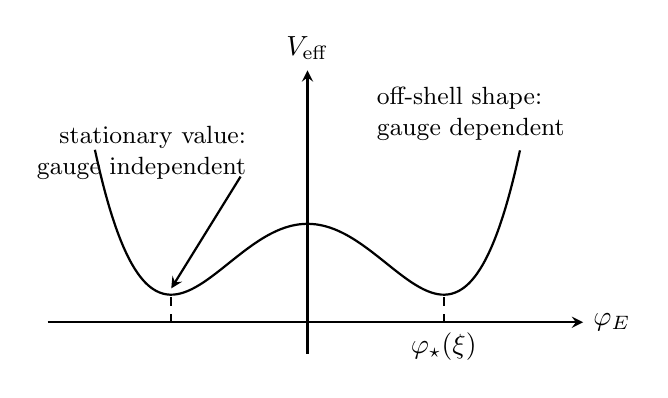
\begin{tikzpicture}[>=stealth,thick,line label/.style={fill=white,fill opacity=.96,text opacity=1,inner sep=1.15pt}]
\draw[->] (-3.3,0) -- (3.5,0) node[right]{$\varphi_E$};
\draw[->] (0,-.4) -- (0,3.2) node[above]{$V_{\rm eff}$};
\draw[smooth,domain=-2.7:2.7,samples=120] plot (\x,{0.10*(\x*\x-3)^2+0.35});
\draw[dashed] (-1.73,0)--(-1.73,.35);
\draw[dashed] (1.73,0)--(1.73,.35);
\node[below] at (1.73,0){$\varphi_\star(\xi)$};
\node[align=left,anchor=west,font=\small] at (0.75,2.65){off-shell shape:\\gauge dependent};
\node[align=right,anchor=east,font=\small] at (-0.65,2.15){stationary value:\\gauge independent};
\draw[->] (-0.85,1.85)--(-1.73,.43);
\end{tikzpicture}
\caption{有效势是离壳 1PI 对象，其曲线形状和驻点坐标一般依赖规范固定参数。Nielsen 恒等式保证量子驻点处的有效作用量值不随规范参数改变；物理质量仍需由完整极点条件定义。}
\label{fig:sm-nielsen-effective-potential-dp12}
\end{figure}

真空稳定性的微扰陈述必须同时带有尺度与规范控制。若在给定匹配方案和微扰阶数下，重整化群改进的有效四次耦合在某个能标区域变负，则大场方向可能低于电弱真空；但“$\lambda_{\rm eff}$ 的零点”本身不是严格的规范不变量。真正的可观测结论应通过真空隧穿作用量、寿命或其他规范一致的构造表达，并要求
\begin{equation*}
\epsilon_{\rm loop}
\sim\frac{\max(g_s^2,g^2,g'^2,y_t^2,\lambda_H)}{16\pi^2}\ll1,
\qquad
\left|\ln\frac{\varphi_E}{E_{\rm R}}\right|=\mathcal O(1),
\end{equation*}
否则必须加入更高圈重整化群改进或非微扰信息。


当新的重自由度位于远高于实验动量的尺度时，低能实验不能直接产生这些重态，但它们的虚过程仍会改变只由标准模型轻场构成的局域相互作用。量子场论的一般有效场论框架已经说明：把高能自由度消去以后，应按算符维数排列这些局域修正，并用 Wilson 系数记录被消去的短距离动力学。把这一构造专门限制在标准模型的场内容和 $SU(3)_c\times SU(2)_L\times U(1)_Y$ 规范对称性上，所得低能理论称为\emph{标准模型有效场论}（Standard Model Effective Field Theory，SMEFT）。

最小可重整化标准模型的场内容和规范对称性已经固定，因此更高能自由度在低能留下的局域效应可以直接专门化量子场论的一般有效场论母\eqnrefs{eq:eft-operator-suppression-dp10}。沿用\eqnrefs{eq:qft-eft-three-scales-dp42} 的逆长度尺度 $\Lambda_*$、物理动量尺度 $p_*=\hbar\Lambda_*$ 与能量尺度 $\Lambda_E=\hbar c\Lambda_*$，其拉氏量写成
\begin{equation}
\boxed{
\widehat\Lag_{\rm SMEFT}
=\widehat\Lag_{\rm SM}
+\sum_{d>4}\frac{C_i^{(d)}}{\Lambda_*^{d-4}}
\widehat{\mathcal O}_i^{(d)}.}
\label{eq:smeft-specialization-dp42}
\end{equation}
其中 $[\widehat{\mathcal O}_i^{(d)}]=\mathrm{m^{-d}}$，Wilson 系数 $C_i^{(d)}$ 无量纲。若过程的特征物理四动量为 $Q$，局域展开的控制量是 $Q/p_*=Qc/\Lambda_E$，不能把 $Q$ 直接与逆长度 $\Lambda_*$ 比较。

在标准模型轻场中，若要求保持规范对称性和重子数、但允许轻子数改变，最低维的非重整化局域结构必须同时包含两个左手轻子二重态和两个 Higgs 场。两个轻子场使它改变两单位轻子数，两个 Higgs 场则补足弱同位旋与超荷，使整个乘积成为规范单态。其拉氏量可以写成
\begin{equation}
\boxed{
\Delta\Lag_5
=-\frac{\hbar c}{2\Lambda_*}C_{ij}^{(5)}
\left(\overline{L_{Li}^{\,c}}\,\widetilde\Phi^*\right)
\left(\widetilde\Phi^\dagger L_{Lj}\right)
+\mathrm{H.c.}}
\label{eq:weinberg-operator-dp11}
\end{equation}
其中 $C_{ij}^{(5)}$ 是味空间中的对称系数矩阵。\eqnrefs{eq:weinberg-operator-dp11} 是标准模型轻场能够写出的唯一维数五规范不变结构，通常称为\emph{Weinberg 算符}。

Higgs 场取得真空期望值后，两个 Higgs 因子被 $v_E$ 替代，\eqnrefs{eq:weinberg-operator-dp11} 于是直接把左手中微子场与它的电荷共轭场配对。与普通 Dirac 质量不同，这里不需要一个独立的右手中微子场，而且该质量项改变两单位轻子数；对中性费米子，这种“场与自身电荷共轭配对”的质量称为\emph{Majorana 质量}。其味空间质量矩阵为复对称矩阵，并具有量级
\begin{equation}
\boxed{
M_\nu c^2\sim C^{(5)}\frac{v_E^2}{\Lambda_E}.}
\label{eq:neutrino-mass-weinberg-dp11}
\end{equation}
因此极小的中微子质量可以对应远高于电弱尺度的 $\Lambda_E$，也可以来自较小的 Wilson 系数；仅凭低能质量本身不能唯一反推出高能机制。

普通厄米矩阵由相似变换对角化，但 Majorana 质量矩阵满足的是复对称条件 $M_\nu^T=M_\nu$，并不要求 $M_\nu^\dagger=M_\nu$。对于任意复对称矩阵，存在一个幺正矩阵 $U_\nu$，使幺正\emph{合同变换}而不是相似变换将其化为非负实对角矩阵：
\begin{equation*}
U_\nu^TM_\nu U_\nu=M_\nu^{\rm diag},
\qquad M_\nu^{\rm diag}=\operatorname{diag}(m_1,m_2,m_3),\quad m_i\ge0.
\end{equation*}
这种复对称矩阵的幺正合同对角化称为\emph{Takagi 分解}。它定义中微子的质量本征基；带电轻子的左手质量基变换记为 $U_{eL}$。带电流同时比较带电轻子的左手质量基与中微子的质量基，因此只留下二者的相对幺正变换。这个矩阵称为 Pontecorvo--Maki--Nakagawa--Sakata（PMNS）矩阵，定义为
\begin{equation}
\boxed{U_{\rm PMNS}=U_{eL}^\dagger U_\nu.}
\label{eq:pmns-definition-dp11}
\end{equation}
这与 CKM 矩阵的来源具有相同的“两个质量扇区左手旋转不一致”结构；Majorana 相位则只有在破坏轻子数的可观测量中才可能显现。定义完成以后，轻子带电流在质量本征基中成为
\begin{equation}
\boxed{
 \Lag_{\rm CC}^{\ell}
 =-\frac{\hbar c\,g}{\sqrt2}
 \left[\bar\nu_i\gamma^\mu P_L(U_{\rm PMNS})_{\alpha i}^*\ell_\alpha\,\mathcal W_\mu^+
 +\mathrm{H.c.}\right],}
\label{eq:pmns-charged-current-dp43}
\end{equation}
这里 $\alpha=e,\mu,\tau$ 标记带电轻子质量本征态，$i=1,2,3$ 标记中微子质量本征态，重复指标求和。$W^+$ 项的矩阵是 $U_\nu^\dagger U_{eL}=U_{\rm PMNS}^\dagger$，所以相应的约化 $W^+\nu_i\bar\ell_\alpha$ 顶角为 $-\ii g(U_{\rm PMNS})_{\alpha i}^*\gamma^\mu P_L/\sqrt2$；厄米共轭的 $W^-$ 项含 $U_{\alpha i}$。因此 PMNS 只在中微子质量机制已经引入并完成两套左手质量基对角化之后出现。

对相干的超相对论传播，定义
\begin{equation*}
\Delta_{ij}\equiv\frac{\Delta m_{ij}^2c^3L}{4E\hbar},
\qquad
K_{ij}^{\alpha\beta}
\equiv U_{\alpha i}^*U_{\beta i}U_{\alpha j}U_{\beta j}^*,
\end{equation*}
三味真空振荡概率为
\begin{equation}
\boxed{
P_{\alpha\to\beta}(L,E)
=\delta_{\alpha\beta}
-4\sum_{i<j}\Re K_{ij}^{\alpha\beta}\sin^2\Delta_{ij}
+2\sum_{i<j}\Im K_{ij}^{\alpha\beta}\sin(2\Delta_{ij}).}
\label{eq:neutrino-oscillation-probability-dp14}
\end{equation}
这里 $L$ 是源到探测器的传播基线，$E$ 是共同的主导能量，$\Delta m_{ij}^2=m_i^2-m_j^2$。第一类项在中微子与反中微子之间不变；第二类在 $U\to U^*$ 时变号，因此承载 CP 奇的干涉信息。该公式要求 $m_i^2c^4/E^2\ll1$，并要求不同质量本征波包在传播距离 $L$ 上仍有显著空间重叠；波包完全分离后，非对角干涉项会退相干。

\begin{figure}[htbp]
\centering

\includegraphics[width=.76\textwidth]{sm_neutrino_oscillation_dp11.png}
\caption{三味真空中微子振荡示意。横轴采用 $\Delta_{31}=\Delta m_{31}^2c^3L/(4E\hbar)$；混合角、CP 相位和 $\Delta m_{21}^2/\Delta m_{31}^2$ 取代表值，只用于显示三个质量本征相位的干涉。虚线 $\sum_\beta P_{\mu\to\beta}=1$ 检验 PMNS 幺正性。}
\label{fig:sm-neutrino-oscillation-dp11}
\end{figure}

有效场论中的 Wilson 系数必须由高能理论的自由度和耦合决定，而不能仅凭低能算符的维数猜测。对任何在给定背景下只以二次型出现的重场，树级匹配首先是一个分块算符消元问题。把轻、重自由度组成列向量，并把二次核写成
\begin{equation*}
 \mathcal K(p)=
 \begin{pmatrix}
  K_{LL}(p)&K_{LH}(p)\\
  K_{HL}(p)&K_{HH}(p)
 \end{pmatrix}.
\end{equation*}
若过程能区内 $K_{HH}(p)$ 可逆，则消去重块以后，轻场的精确二次核为 Schur 补
\begin{equation}
 \boxed{
 K_{\rm eff}(p)
 =K_{LL}(p)-K_{LH}(p)K_{HH}^{-1}(p)K_{HL}(p).}
 \label{eq:sm-heavy-block-schur-matching-dp85}
\end{equation}
\eqnrefs{eq:sm-heavy-block-schur-matching-dp85} 保留 $K_{HH}^{-1}(p)$ 的完整动量依赖，是局域 EFT 展开之前的精确二次型母式。

设重块的最小质量能隙为 $M_{H,\min}^{(E)}$，过程特征能量为 $Q_E$。只有在
\begin{equation}
 \boxed{
 \epsilon_H\equiv\frac{Q_E}{M_{H,\min}^{(E)}}\ll1}
 \label{eq:sm-heavy-field-local-control-dp85}
\end{equation}
时，才可把重传播子按外部动量展开成局域算符级数。最低阶保留 $K_{HH}^{-1}(0)$，更高阶项依次带额外的 $Q_E/M_H^{(E)}$ 幂；这正是从一个确定 UV 理论得到低能 Wilson 系数的树级匹配程序。

\begin{exbox}[重右手中微子与 type-I seesaw]
在标准模型轻场之外加入规范单态右手中微子 $N_R$。沿用全书 Higgs--Yukawa 的 SI 归一化，其新增拉氏量为
\begin{equation*}
 \Delta\Lag_N
 =-\sqrt{\hbar c}\,\overline{L_L}Y_\nu\widetilde\Phi N_R
 -\frac{\hbar c}{2}\overline{N_R^{\,c}}\,\widehat M_R N_R
 +\mathrm{H.c.},
\end{equation*}
其中 $Y_\nu$ 是无量纲 Yukawa 矩阵，$\widehat M_R$ 具有逆长度量纲，并定义质量能量矩阵
\begin{equation*}
 M_R^{(E)}\equiv\hbar c\,\widehat M_R.
\end{equation*}
令
\begin{equation*}
 M_{R,\min}^{(E)}\equiv\sigma_{\min}(M_R^{(E)}),
 \qquad
 \epsilon_R\equiv\frac{Q_E}{M_{R,\min}^{(E)}}\ll1.
\end{equation*}
\eqnrefs{eq:sm-heavy-block-schur-matching-dp85} 中重 Majorana 传播子的轻--轻手征翻转部分在最低阶给出 $(M_R^{(E)})^{-1}$。代入两个 Yukawa 顶角，Weinberg 算符的能量归一化系数为
\begin{equation}
 \boxed{
 \frac{C^{(5)}}{\Lambda_E}
 =Y_\nu(M_R^{(E)})^{-1}Y_\nu^T+\delta C_5,
 \qquad
 \frac{\|\delta C_5\|}
 {\|Y_\nu\|^2\,\|(M_R^{(E)})^{-1}\|}
 =O(\epsilon_R^2).}
 \label{eq:typeI-weinberg-matching-dp86}
\end{equation}
Higgs 场取得真空期望值以后，$m_Dc^2=v_EY_\nu/\sqrt2$，轻中微子质量矩阵变成
\begin{equation}
 \boxed{
 M_\nu c^2
 =-\frac{v_E^2}{2}
 Y_\nu(M_R^{(E)})^{-1}Y_\nu^T
 +O\!\left(\frac{\|m_Dc^2\|^4}{[M_{R,\min}^{(E)}]^3}\right).}
 \label{eq:typeI-seesaw-mass-dp86}
\end{equation}
不同 UV 理论可以匹配到同一个 Weinberg 系数；type-I seesaw 对应其中由重 Majorana 单态产生的一组 Wilson 系数。
\end{exbox}


维数升到六以后，满足规范对称性的局域算符迅速增多，其中一些却通过分部积分、经典运动方程或 Fierz 恒等式彼此等价。把这些冗余关系商掉以后，留下的独立局域结构构成\emph{算符基}。

不同算符基只是同一算符空间的不同坐标系；Wilson 系数随基变换而改变，但同一截断精度下的可观测振幅不能依赖这种坐标选择。与 Higgs、电弱精密观测和半轻子过程直接相关的代表性结构为
\begin{align*}
\mathcal O_H&=(\Phi^\dagger\Phi)^3,\\
\mathcal O_{H\Box}&=(\Phi^\dagger\Phi)\Box(\Phi^\dagger\Phi),\\
\mathcal O_{HD}&=(\Phi^\dagger D_\mu\Phi)^*(\Phi^\dagger D^\mu\Phi),\\
\mathcal O_{HB}&=(\Phi^\dagger\Phi)\mathcal B_{\mu\nu}\mathcal B^{\mu\nu},\\
\mathcal O_{HW}&=(\Phi^\dagger\Phi)\mathcal W_{\mu\nu}^I\mathcal W^{I\mu\nu},\\
\mathcal O_{HWB}&=(\Phi^\dagger\sigma^I\Phi)\mathcal W_{\mu\nu}^I\mathcal B^{\mu\nu},\\
\mathcal O_{\ell q}^{(3)}
&=(\bar L\gamma_\mu\sigma^IL)(\bar Q\gamma^\mu\sigma^IQ).
\end{align*}
$\mathcal O_H$ 改变 Higgs 势，$\mathcal O_{H\Box}$ 与 $\mathcal O_{HD}$ 改变 Higgs 动力学及质量--耦合关系，$\mathcal O_{HB},\mathcal O_{HW},\mathcal O_{HWB}$ 改变 Higgs 与规范场以及中性规范场混合，$\mathcal O_{\ell q}^{(3)}$ 则直接修正半轻子带电流和中性流。特别地，$\mathcal O_{HD}$ 对前面定义的守护对称性质量关系敏感，$\mathcal O_{HWB}$ 改变 $W^3$--$B$ 混合；因此把精密电弱数据翻译为这两个 Wilson 系数时，必须同时指定输入参数方案并做规范场的重新归一化，不能只在某一条树级质量公式上“加一个修正项”。

算符基必须利用分部积分、经典运动方程、Fierz 恒等式和厄米共轭关系去除冗余。不同基底之间的 Wilson 系数可以不同，但同一精度下的物理振幅必须一致；因此“列出所有看似规范不变的高维项”并不能定义一个可用于匹配和运行的独立算符基。

截断到六维要求过程中的特征不变量能量满足
\begin{equation*}
\epsilon_{\rm EFT}\equiv\frac{E_{\rm inv}^2}{\Lambda_E^2}\ll1.
\end{equation*}
若计算只保留标准模型振幅与六维振幅的 $1/\Lambda_E^2$ 干涉项，却丢弃六维振幅平方，则还必须检查 $|\mathcal M_{d6}|^2/\Lambda_E^4$ 相对于未知八维干涉确实可忽略。强耦合高能完成、选择定则造成的低阶抑制或异常大的 Wilson 系数都会改变朴素幂次计数，因此有效场论误差必须针对具体可观测量分别报告局域展开、匹配截断和重整化群截断三部分。


低能弱衰变中的局域四费米子算符和中微子质量中的 Weinberg 算符都体现同一机制：不可直接产生的高能自由度被积分掉，其影响留在局域算符的 Wilson 系数中。六维标准模型有效场论把这一机制推广到 Higgs、规范场和费米子过程。独立算符基描述低能自由度，阈值匹配确定 Wilson 系数的高能边界值，重整化群方程把这些系数演化到实验尺度，低能矩阵元再把它们转化为可观测量。局域展开、匹配截断和重整化群截断因此是三种独立误差来源。


量子场论的一般有效场论母式在标准模型场内容上的专门化由\eqnrefs{eq:smeft-specialization-dp42} 给出。六维匹配还需要把同一重尺度写成物理四动量的量纲，因此定义匹配动量尺度
\begin{equation}
\boxed{\mu_{\rm M}\equiv\hbar\Lambda_*=\frac{\Lambda_E}{c}},
\qquad [\mu_{\rm M}]=\mathrm{kg\,m\,s^{-1}}.
\label{eq:smeft-matching-momentum-dp13}
\end{equation}
于是逆长度、动量与能量分别由 $\Lambda_*$、$\mu_{\rm M}$ 与 $\Lambda_E$ 表示，不会在对数或重整化群方程中混用。配合 $\widehat\Phi=\Phi/\sqrt{\hbar c}$、$[\psi]=\mathrm{m^{-3/2}}$ 与 $[\mathscr C_\mu]=\mathrm{m^{-1}}$，\eqnrefs{eq:smeft-specialization-dp42} 在 $d=6$ 时给出

若 $\widehat{\mathcal O}_i^{(6)}$ 的几何量纲为 $\mathrm{m^{-6}}$，则
\begin{align}
\Delta\widehat\Lag_6
&=\sum_i\frac{C_i^{(6)}}{\Lambda_*^2}\widehat{\mathcal O}_i^{(6)},
\label{eq:smeft-geometric-normalization-dp13}\\
\Delta\Lag_6
&=\frac{(\hbar c)^3}{\Lambda_E^2}
\sum_iC_i^{(6)}\widehat{\mathcal O}_i^{(6)}.
\label{eq:smeft-si-normalization-dp13}
\end{align}
因此 $C_i^{(6)}$ 全部无量纲。例如 $\widehat{\mathcal O}_H=(\widehat\Phi^\dagger\widehat\Phi)^3$ 对应
\begin{equation*}
\Delta\Lag_H=\frac{C_H}{\Lambda_E^2}(\Phi^\dagger\Phi)^3,
\end{equation*}
单位为 $\mathrm{J\,m^{-3}}$。该几何归一化仅重排幂次计数，所有系数继续保持上述 SI 量纲。


匹配的精确定义是把重场 $H$ 在保持轻场 $\ell$ 外部背景的条件下积分掉：
\begin{equation}
\boxed{
\exp\!\left[\frac{\ii}{\hbar}\Gamma_{\rm LE}[\ell]\right]
=\int\mathcal D H\,
\exp\!\left[\frac{\ii}{\hbar}S_{\rm UV}[\ell,H]\right].}
\label{eq:smeft-matching-functional-dp32}
\end{equation}
该泛函积分定义精确而一般非局域的低能作用量；只有在外部不变量远小于重质量后，对重传播子作预解式展开，才得到局域算符级数。分块二次核\eqnrefs{eq:sm-heavy-block-schur-matching-dp85} 给出一般 Schur 母式。对线性源耦合的二次重场块
\begin{equation*}
\widehat\Lag_{\rm UV}
=\widehat\Lag_{\rm light}+\frac12H\mathsf K_HH+H\mathcal J[\ell],
\end{equation*}
重场方程 $\mathsf K_HH+\mathcal J=0$ 给出 $H_{\rm cl}=-\mathsf K_H^{-1}\mathcal J$；代回二次型，树级低能项立即成为
\begin{equation}
\boxed{
\Delta\widehat\Lag_{\rm LE}^{\rm tree}
=-\frac12\mathcal J\mathsf K_H^{-1}\mathcal J.}
\label{eq:smeft-tree-resolvent-dp32}
\end{equation}
若 $\mathsf K_H=\Lambda_*^2+\mathsf D$，并且在所考察低能态空间内 $\|\mathsf D\|/\Lambda_*^2\ll1$，则重传播子的逆算符可按无量纲小量 $\mathsf D/\Lambda_*^2$ 展开：
\begin{equation}
\boxed{
\mathsf K_H^{-1}
=\frac1{\Lambda_*^2}
\left[
 I-\frac{\mathsf D}{\Lambda_*^2}
 +O\!\left(\frac{\mathsf D^2}{\Lambda_*^4}\right)
\right],
\qquad
\epsilon_{\rm EFT}
\sim\frac{E_{\rm inv}^2}{\Lambda_E^2}\ll1.}
\label{eq:smeft-heavy-resolvent-expansion-dp76}
\end{equation}
第一项产生六维局域算符，下一项产生多两个导数的八维结构，因此有效场论的局域截断就是重传播子的受控低能展开。这里的 $\epsilon_{\rm EFT}\sim E_{\rm inv}^2/\Lambda_E^2$ 是二阶微分重块的具体幂次计数；它是一般控制量\eqnrefs{eq:sm-heavy-field-local-control-dp85} 在该传播子结构下的特化。

\begin{figure}[htbp]
\centering
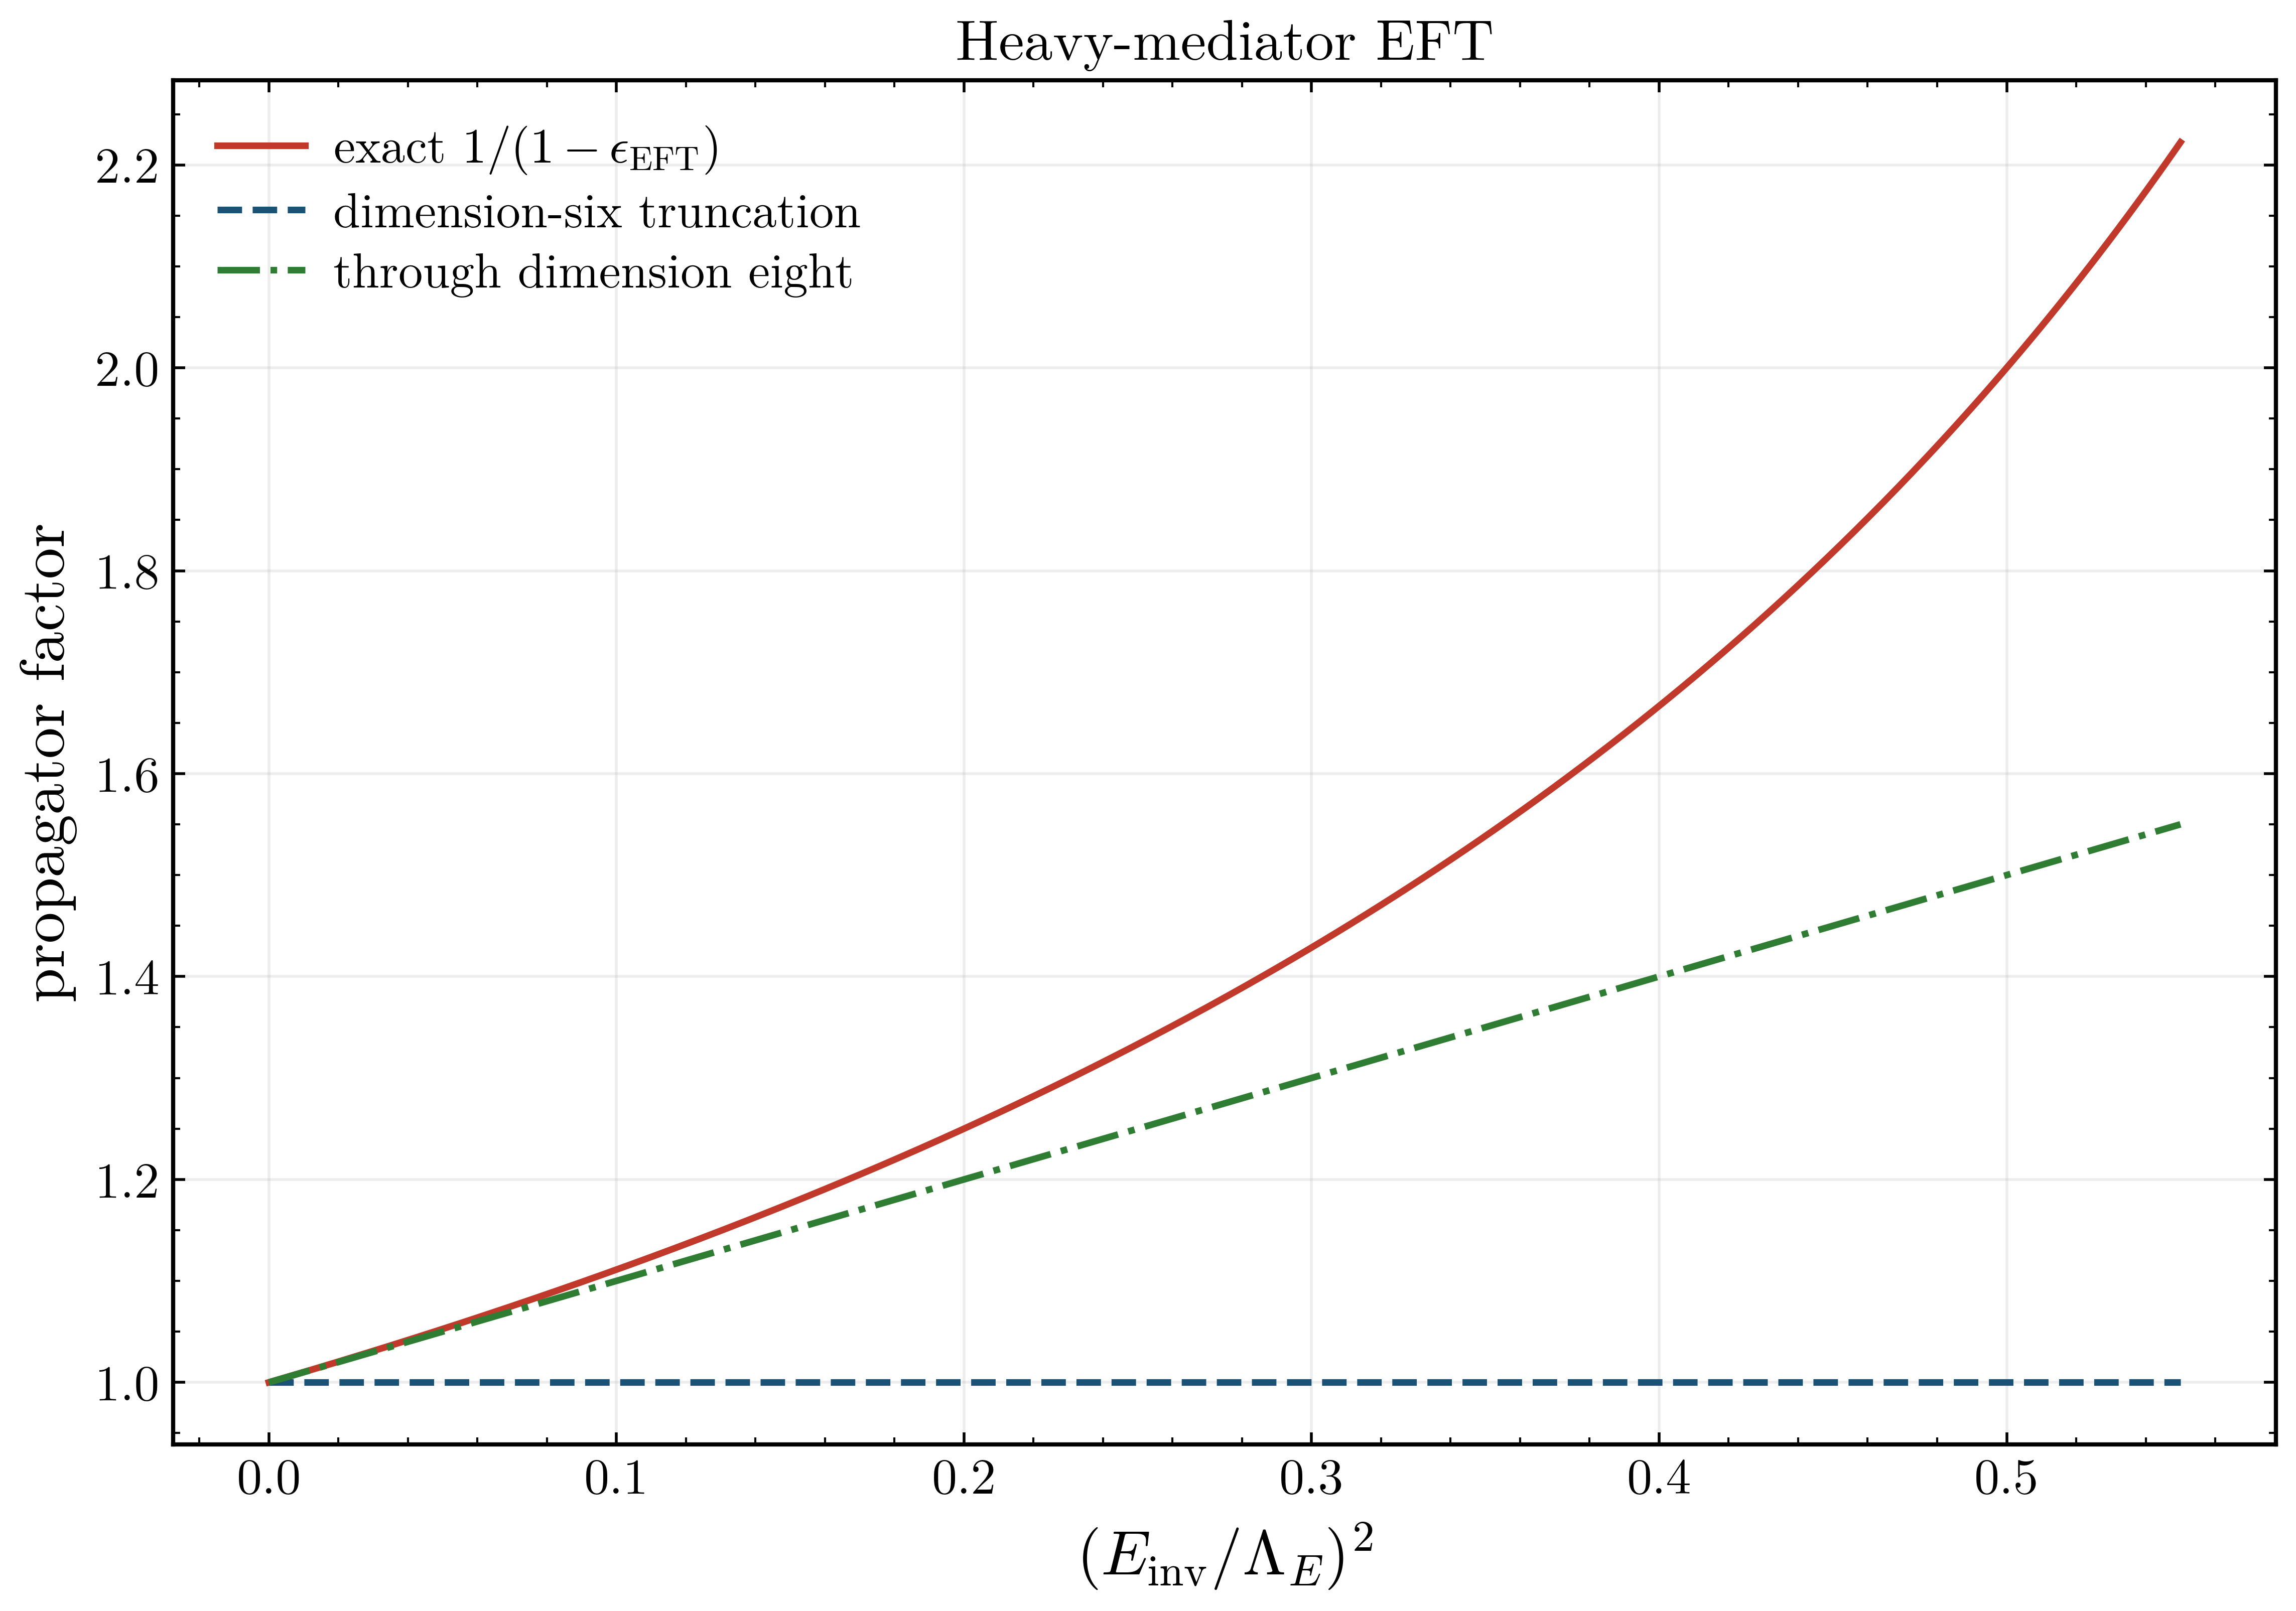
\includegraphics[width=.76\linewidth]{content/FreeElectronQuantumOptics/figures/generated/smeft_propagator_expansion_dp13.png}
\caption{重传播子的局域展开。六维截断只保留预解式的第一项；加入八维项后恢复首个 $E_{\rm inv}^2/\Lambda_E^2$ 修正。随着 $E_{\rm inv}/\Lambda_E$ 增大，有限阶局域展开逐渐失去精度。}
\label{fig:smeft-propagator-expansion-dp13}
\end{figure}

\begin{exbox}[重单态矢量场的树级匹配]
考虑质量尺度为 $\Lambda_*$ 的实矢量场 $X_\mu$，它只耦合到两个标准模型规范单态流
\begin{equation*}
J_L^\mu\equiv\bar L\gamma^\mu L,
\qquad
J_Q^\mu\equiv\bar Q\gamma^\mu Q,
\end{equation*}
并取
\begin{equation}
\widehat\Lag_X
=-\frac14X_{\mu\nu}X^{\mu\nu}
+\frac12\Lambda_*^2X_\mu X^\mu
-X_\mu(g_LJ_L^\mu+g_QJ_Q^\mu).
\label{eq:heavy-vector-uv-lag-dp13}
\end{equation}
记
\begin{equation*}
J_X^\mu\equiv g_LJ_L^\mu+g_QJ_Q^\mu.
\end{equation*}
对 $X_\mu$ 变分得到经典场方程。对守恒外流，纵向传播部分不贡献最低阶局域匹配；在动量空间只需保留横向块，于是
\begin{equation*}
\left(\Lambda_*^2-\frac{q^2}{\hbar^2}\right)X^\mu(q)=J_X^\mu(q),
\end{equation*}
从而
\begin{equation*}
X^\mu(q)
=\frac{J_X^\mu(q)}{\Lambda_*^2-q^2/\hbar^2}
=\frac{J_X^\mu(q)}{\Lambda_*^2}
\left[1+O\!\left(\frac{E_{\rm inv}^2}{\Lambda_E^2}\right)\right].
\end{equation*}
当 $E_{\rm inv}\ll\Lambda_E$ 时，把最低阶经典解 $X^\mu\simeq J_X^\mu/\Lambda_*^2$ 代回二次项与源项：
\begin{align*}
\frac12\Lambda_*^2X_\mu X^\mu-X_\mu J_X^\mu
&=\frac{1}{2\Lambda_*^2}J_{X\mu}J_X^\mu
-\frac{1}{\Lambda_*^2}J_{X\mu}J_X^\mu\\
&=-\frac{1}{2\Lambda_*^2}J_{X\mu}J_X^\mu.
\end{align*}
再展开流的平方，
\begin{align*}
J_{X\mu}J_X^\mu
&=(g_LJ_{L\mu}+g_QJ_{Q\mu})
  (g_LJ_L^\mu+g_QJ_Q^\mu)\\
&=g_L^2J_{L\mu}J_L^\mu
 +2g_Lg_QJ_{L\mu}J_Q^\mu
 +g_Q^2J_{Q\mu}J_Q^\mu.
\end{align*}
因此六维低能拉氏量中的三个四费米子结构分别得到
\begin{equation*}
\Delta\widehat\Lag_6
=\frac1{\Lambda_*^2}
\left[
-\frac{g_L^2}{2}J_L^2
-g_Lg_QJ_L\!\cdot J_Q
-\frac{g_Q^2}{2}J_Q^2
\right]
+O\!\left(\frac{E_{\rm inv}^2}{\Lambda_E^2}\right),
\end{equation*}
所以匹配尺度上的无量纲 Wilson 系数为
\begin{equation}
\boxed{
C_{\ell\ell}^{(1)}=-\frac{g_L^2}{2},
\qquad
C_{\ell q}^{(1)}=-g_Lg_Q,
\qquad
C_{qq}^{(1)}=-\frac{g_Q^2}{2}.}
\label{eq:heavy-vector-wilson-matching-dp13}
\end{equation}
三个系数不是三个任意参数：一个重矢量只提供 $g_L$、$g_Q$ 两个耦合，因此它们满足
\begin{equation*}
\bigl(C_{\ell q}^{(1)}\bigr)^2
=4C_{\ell\ell}^{(1)}C_{qq}^{(1)}.
\end{equation*}
这个关系给出了可直接用于低能拟合的模型检验；若实验提取的三个 Wilson 系数显著不满足它，就不能由这一单一重矢量在树级独自解释。
\end{exbox}

树级匹配并不是唯一来源。如果重实标量 $S$ 通过 $\kappa S^2(\widehat\Phi^\dagger\widehat\Phi)/2$ 与 Higgs 耦合，而且树级经典解为 $S=0$，那么 $\mathcal O_H=(\Phi^\dagger\Phi)^3$ 的第一项从一圈泛函行列式产生。按\eqnrefs{eq:smeft-geometric-normalization-dp13} 的归一化，匹配尺度上的结果为
\begin{equation}
\boxed{
C_H(\mu_{\rm M})=-\frac{\kappa^3}{192\pi^2}.}
\label{eq:heavy-scalar-ch-loop-dp32}
\end{equation}
这里 $1/(16\pi^2)$ 的环抑制和 $1/\Lambda_E^2$ 的局域展开抑制是两个独立层级；不能用一个“有效场论小参数”同时代表二者。

匹配只固定某一尺度上的 Wilson 系数。先把复合算符的重整化混合定义为
\begin{equation}
 \mu_{\rm DR}\frac{\dd\widehat{\mathbf O}}{\dd\mu_{\rm DR}}
 =-\gamma^{\mathcal O}\widehat{\mathbf O}.
 \label{eq:smeft-operator-rg-dp68}
\end{equation}
物理有效拉格朗日量中的组合 $\mathbf C^T\widehat{\mathbf O}$ 不能依赖辅助尺度，因此系数向量必须按相反的转置矩阵作用运行：
\begin{equation}
\boxed{
\mu_{\rm DR}\frac{\dd\mathbf C}{\dd\mu_{\rm DR}}
=(\gamma^{\mathcal O})^T\mathbf C.}
\label{eq:smeft-wilson-rg-dp32}
\end{equation}
当不同尺度上的反常维数矩阵不彼此对易时，不能把它们当成一个常矩阵直接指数化。令 $t=\ln\mu_{\rm DR}$，从匹配尺度 $\mu_{\rm M}$ 演化到任意低能尺度的形式解为
\begin{equation}
\boxed{
\mathbf C(\mu_{\rm DR})
=\mathcal P\exp\!\left[
\int_{\ln\mu_{\rm M}}^{\ln\mu_{\rm DR}}\dd\ell\,
(\gamma^{\mathcal O}(\ell))^T
\right]\mathbf C(\mu_{\rm M}),}
\label{eq:smeft-wilson-evolution-dp90}
\end{equation}
其中 $\mathcal P$ 按尺度参数 $\ell$ 排序；只有当 $[(\gamma^{\mathcal O}(\ell_1))^T,(\gamma^{\mathcal O}(\ell_2))^T]=0$ 时，路径有序符号才可以去掉。
因此某个系数在匹配尺度上为零，并不意味着它在实验尺度上仍为零；只要反常维数矩阵存在非对角元，运行就会生成与原算符发生混合的其他系数。这也是低能算符子空间必须对重整化闭合的原因。

Weinberg 算符的一圈重整化同时涉及普适缩放和味非普适混合。沿用\eqnrefs{eq:sm-higgs-quartic-beta-dp93} 前已经定义的味普适迹 $\mathcal T_Y$，这里只需再定义作用在左手轻子二重态味空间的矩阵
\begin{equation*}
 \mathcal Y_L\equiv Y_eY_e^\dagger.
\end{equation*}
这个左右次序由 Yukawa 项 $\bar L_LY_e\Phi e_R$ 的指标位置固定；$\mathcal T_Y$ 则继续表示全部标准模型 Yukawa 耦合对 Higgs 波函数重整化产生的味普适迹。取 $d=4-2\epsilon$，由于\eqnrefs{eq:weinberg-operator-dp11} 含两个 $L_L$ 和两个 $\Phi$ 外腿，裸系数与重整化系数的矩阵关系必须写成
\begin{equation}
\boxed{
 C_B^{(5)}
 =\mu_{\rm DR}^{2\epsilon} Z_\Phi^{-1}
 (Z_L^T)^{-1/2}
 \left[C^{(5)}+\delta C^{(5)}\right]
 Z_L^{-1/2}.}
\label{eq:weinberg-bare-renorm-dp91}
\end{equation}
这里 $Z_L$ 是左手轻子二重态的味空间波函数重整化矩阵，$Z_\Phi$ 是 Higgs 二重态的波函数重整化常数，$\delta C^{(5)}$ 是四点 1PI 顶角的局域反项。矩阵因子的左右次序不能交换；它正是 Weinberg 系数保持复对称性的原因。

在 $Q=T_3+Y$ 的超荷约定和\eqnrefs{eq:sm-higgs-lagrangian-dp11} 的 Higgs 势
$V=-\mu_H^2\Phi^\dagger\Phi+\lambda_H(\Phi^\dagger\Phi)^2/(\hbar c)$ 归一化下，一圈标准模型运行最终为
\begin{align}
16\pi^2\mu_{\rm DR}\frac{\dd C^{(5)}}{\dd\mu_{\rm DR}}
={}&\left[4\lambda_H-3g^2+2\mathcal T_Y\right]C^{(5)}\nonumber\\
&-\frac32\left[\mathcal Y_L^T C^{(5)}+C^{(5)}\mathcal Y_L\right].
\label{eq:weinberg-matrix-rg-dp32}
\end{align}
$4\lambda_H-3g^2+2\mathcal T_Y$ 只改变味矩阵的整体缩放；$\mathcal Y_L^TC^{(5)}+C^{(5)}\mathcal Y_L$ 则沿带电轻子 Yukawa 的左手味方向产生非普适形变。因而跨越很大的能标区间时，中微子质量的整体尺度和 PMNS 参数都可能运行。

\begin{figure}[htbp]
\centering
\begin{tikzpicture}[>=Latex,node distance=13mm and 14mm,line label/.style={fill=white,fill opacity=.96,text opacity=1,inner sep=1.15pt}]
\node[draw,rounded corners,align=center,minimum width=34mm,minimum height=13mm] (uv) {UV theory\\light $+$ heavy fields};
\node[draw,rounded corners,align=center,right=of uv,minimum width=31mm,minimum height=13mm] (match) {threshold matching\\$E\sim\Lambda_E$};
\node[draw,rounded corners,align=center,right=of match,minimum width=34mm,minimum height=13mm] (wilson) {$C_i(\Lambda_E)$\\local operators};
\node[draw,rounded corners,align=center,below=of wilson,minimum width=34mm,minimum height=13mm] (rg) {$\gamma_{ij}$\\operator mixing};
\node[draw,rounded corners,align=center,left=of rg,minimum width=31mm,minimum height=13mm] (low) {$C_i(E)$\\experimental scale};
\node[draw,rounded corners,align=center,left=of low,minimum width=34mm,minimum height=13mm] (obs) {observable\\SM $+$ EFT};
\draw[->,thick] (uv)--node[line label,midway,above,font=\scriptsize]{integrate out heavy modes}(match);
\draw[->,thick] (match)--node[line label,midway,above,font=\scriptsize]{boundary conditions}(wilson);
\draw[->,thick] (wilson)--node[line label,midway,right,font=\scriptsize]{anomalous dimensions}(rg);
\draw[->,thick] (rg)--node[line label,midway,below,font=\scriptsize]{RG evolution / log resummation}(low);
\draw[->,thick] (low)--(obs);
\end{tikzpicture}
\caption{有效场论的单向计算链。高能阈值决定匹配条件，算符反常维数矩阵把 Wilson 系数运行到实验尺度，最后才与低能矩阵元组合成可观测量。}
\label{fig:smeft-matching-running-chain-dp13}
\end{figure}

局域截断由 $\epsilon_{\rm EFT}=E_{\rm inv}^2/\Lambda_E^2\ll1$ 控制；匹配的环截断由 $g_*^2/(16\pi^2)$、$g_s^2/(16\pi^2)$ 等参数控制；重整化群截断则由反常维数的环展开控制。若 $|\ln(\Lambda_E/E)|\gg1$，即使耦合很小，固定阶中的 $g^2\ln(\Lambda_E/E)/(16\pi^2)$ 也可能达到一阶，此时必须在高能阈值先做匹配，再用重整化群重求和到实验尺度。


标准模型有效场论的计算顺序由四个彼此不同的步骤组成：重场泛函积分定义低能作用量；低能展开把非局域传播子转成局域算符；匹配固定高能阈值处的 Wilson 系数；算符混合再把这些系数运行到实验尺度。树级重矢量场展示了系数相关性，一圈重标量展示了独立的环抑制，Weinberg 算符则展示了真实味矩阵的重整化群形变。



\begin{derivation}[从\eqnrefs{eq:sm-heavy-block-schur-matching-dp85}到\eqnrefs{eq:sm-heavy-field-local-control-dp85}]
把轻、重自由度组成列向量
\begin{equation*}
 \Psi\equiv
 \begin{pmatrix}
  \psi_L\\ \Psi_H
 \end{pmatrix},
\end{equation*}
并把二次型作用量写成
\begin{equation*}
 S_2
 =\frac12\int_p
 \Psi^\dagger(-p)
 \begin{pmatrix}
 K_{LL}(p)&K_{LH}(p)\\
 K_{HL}(p)&K_{HH}(p)
 \end{pmatrix}
 \Psi(p).
\end{equation*}
相应的线性运动方程是
\begin{align*}
 K_{LL}\psi_L+K_{LH}\Psi_H&=0,\\
 K_{HL}\psi_L+K_{HH}\Psi_H&=0.
\end{align*}
只要过程能区内 $K_{HH}(p)$ 可逆，第二式可以精确解为
\begin{equation*}
 \Psi_H=-K_{HH}^{-1}K_{HL}\psi_L.
\end{equation*}
代回第一式：
\begin{align*}
 0
 &=K_{LL}\psi_L+K_{LH}\Psi_H\\
 &=K_{LL}\psi_L
 -K_{LH}K_{HH}^{-1}K_{HL}\psi_L\\
 &=\left(K_{LL}-K_{LH}K_{HH}^{-1}K_{HL}\right)\psi_L.
\end{align*}
因此轻场的精确二次核为
\begin{equation*}
 K_{\rm eff}(p)
 =K_{LL}(p)-K_{LH}(p)K_{HH}^{-1}(p)K_{HL}(p),
\end{equation*}
即正文\eqnrefs{eq:sm-heavy-block-schur-matching-dp85}。

同一个结果也可由分块高斯消元直接验证。定义下三角矩阵
\begin{equation*}
 L=
 \begin{pmatrix}
 I&-K_{LH}K_{HH}^{-1}\\
 0&I
 \end{pmatrix}.
\end{equation*}
则
\begin{align*}
 L
 \begin{pmatrix}
 K_{LL}&K_{LH}\\
 K_{HL}&K_{HH}
 \end{pmatrix}
 &=
 \begin{pmatrix}
 K_{LL}-K_{LH}K_{HH}^{-1}K_{HL}&0\\
 K_{HL}&K_{HH}
 \end{pmatrix}.
\end{align*}
所以 Schur 补不是低能近似，而是对重块可逆这一条件下的精确代数恒等式。

要得到局域 EFT，才需要进一步使用重--轻尺度分离。把重块拆成
\begin{equation*}
 K_{HH}(p)=K_M+\delta K(p),
\end{equation*}
其中 $K_M$ 是由重质量主导、在 $p=0$ 已可逆的部分。提出 $K_M$：
\begin{align*}
 K_{HH}(p)
 &=K_M\left[I+K_M^{-1}\delta K(p)\right].
\end{align*}
定义无量纲算符
\begin{equation*}
 X(p)\equiv K_M^{-1}\delta K(p).
\end{equation*}
若在目标能区内
\begin{equation*}
 \epsilon_{\rm Schur}\equiv\sup_{p\in\mathcal D}\|X(p)\|<1,
\end{equation*}
则 Neumann 级数在算符范数下绝对收敛：
\begin{align*}
 K_{HH}^{-1}(p)
 &=[I+X(p)]^{-1}K_M^{-1}\\
 &=\sum_{n=0}^{\infty}[-X(p)]^nK_M^{-1}.
\end{align*}
截断到 $N$ 阶时，利用有限几何级数恒等式
\begin{equation*}
 [I+X]^{-1}
 =\sum_{n=0}^{N}(-X)^n
 +(-X)^{N+1}[I+X]^{-1},
\end{equation*}
得到预解式余项
\begin{equation*}
 R_{N+1}^{(H)}(p)
 =(-X)^{N+1}[I+X]^{-1}K_M^{-1}.
\end{equation*}
由次乘性和
\begin{equation*}
 \|[I+X]^{-1}\|
 \le\sum_{r=0}^{\infty}\|X\|^r
 \le\frac1{1-\epsilon_{\rm Schur}}
\end{equation*}
可得严格范数界
\begin{equation*}
 \|R_{N+1}^{(H)}(p)\|
 \le
 \|K_M^{-1}\|
 \frac{\epsilon_{\rm Schur}^{N+1}}{1-\epsilon_{\rm Schur}}.
\end{equation*}
代回 Schur 补以后，把预解式级数严格截断到 $X^N$，局域 EFT 二次核为
\begin{align*}
 K_{\rm eff}^{(N)}
 &=K_{LL}
 -K_{LH}
 \left[\sum_{n=0}^{N}(-X)^nK_M^{-1}\right]
 K_{HL}\\
 &=K_{LL}
 -K_{LH}K_M^{-1}K_{HL}
 +K_{LH}XK_M^{-1}K_{HL}\\
 &\quad-K_{LH}X^2K_M^{-1}K_{HL}
 +\cdots
 +(-1)^{N+1}K_{LH}X^NK_M^{-1}K_{HL}.
\end{align*}
这里 $X=K_M^{-1}\delta K$，所以每增加一个 $X$ 就增加一个轻尺度相对于重尺度的幂。精确核与该有限和之差完全由上面的 $R_{N+1}^{(H)}$ 给出，并满足
\begin{equation*}
 \|K_{\rm eff}-K_{\rm eff}^{(N)}\|
 \le
 \|K_{LH}\|\,\|K_{HL}\|\,
 \|K_M^{-1}\|
 \frac{\epsilon_{\rm Schur}^{N+1}}{1-\epsilon_{\rm Schur}}.
\end{equation*}

局域展开的控制量不是单独由一个能量比猜测，而是上面已经定义的算符范数
\begin{equation*}
 \epsilon_{\rm Schur}=\sup_{p\in\mathcal D}\|K_M^{-1}\delta K(p)\|.
\end{equation*}
给定允许的二次核绝对误差 $\delta_K^{\rm tol}>0$，$N$ 阶局域 EFT 在目标能区 $\mathcal D$ 内满足精度要求的充分条件为
\begin{equation*}
 \|K_{LH}\|_{\mathcal D}\,\|K_{HL}\|_{\mathcal D}\,
 \|K_M^{-1}\|
 \frac{\epsilon_{\rm Schur}^{N+1}}{1-\epsilon_{\rm Schur}}
 \le \delta_K^{\rm tol},
 \qquad \epsilon_{\rm Schur}<1,
\end{equation*}
其中 $\|K_{LH}\|_{\mathcal D}\equiv\sup_{p\in\mathcal D}\|K_{LH}(p)\|$，$K_{HL}$ 同理。具体模型中外部能量与重质量之比可以用来估计 $\epsilon_{\rm Schur}$，但可接受性最终由这一算符余项界判定。Schur 补本身始终是精确代数恒等式；截断 Neumann 级数才定义局域 EFT 子模型。
\end{derivation}

\begin{derivation}[从\eqnrefs{eq:ew-onshell-mass-field-ct-dp11}到\eqnrefs{eq:sw-counterterm-massrelation-dp11}]
横向重整化逆传播子写成
\begin{equation*}
 [D_{V,T}(p^2)]^{-1}
 =p^2-m_V^2c^2+\Sigma_{VV,T}^{\rm loop}(p^2)
 -\delta m_V^2c^2+(p^2-m_V^2c^2)\delta Z_V.
\end{equation*}
极点仍位于 $p^2=m_V^2c^2$ 且留数为一，等价于
\begin{align*}
 0&=\Re\widehat\Sigma_{VV,T}(m_V^2c^2)
 \quad\Longrightarrow\quad
 \delta m_V^2c^2=\Re\Sigma_{VV,T}^{\rm loop}(m_V^2c^2),\\
 0&=\Re\widehat\Sigma'_{VV,T}(m_V^2c^2)
 \quad\Longrightarrow\quad
 \delta Z_V=-\Re\Sigma_{VV,T}^{{\rm loop}\,'}(m_V^2c^2),
\end{align*}
即正文\eqnrefs{eq:ew-onshell-mass-field-ct-dp11}。

在壳定义 $s_W^2=1-m_W^2/m_Z^2$ 的一阶变分直接给
\begin{align*}
 2s_W\delta s_W
 &= -\delta\!\left(\frac{m_W^2}{m_Z^2}\right)
 =-c_W^2\left(
 \frac{\delta m_W^2}{m_W^2}-\frac{\delta m_Z^2}{m_Z^2}
 \right),
\end{align*}
因此
\begin{equation*}
 \frac{\delta s_W}{s_W}
 =-\frac{c_W^2}{2s_W^2}
 \left(
 \frac{\delta m_W^2}{m_W^2}-\frac{\delta m_Z^2}{m_Z^2}
 \right),
\end{equation*}
得到正文\eqnrefs{eq:sw-counterterm-massrelation-dp11}。
\end{derivation}



\begin{derivation}[从\eqnrefs{eq:delta-rho-definition-dp11}到\eqnrefs{eq:delta-rho-doublet-dp11}]
记 $F_L=(f_1,f_2)_L^T$、$M_i=m_ic^2$。$\Delta\rho$ 只保留破坏守护 $SU(2)$ 的零动量自能差，因此先抽出共同的 $SU(2)_L$ 耦合并定义
\begin{equation*}
\mathcal I(a,b)
\equiv\mu^{4-d}\!\int\frac{\dd^d\ell_E}{(2\pi)^d}
\frac{\ell_E^2}{(\ell_E^2+a)(\ell_E^2+b)},
\qquad a=M_1^2,\quad b=M_2^2,
\end{equation*}
其中已经 Wick 旋转到欧氏能量动量，$\mu$ 是维数正规化尺度。这个标量积分来自左手流的 Dirac 迹。以异味带电流为例，Minkowski 分子为
\begin{align*}
T^{\mu\nu}_{12}
&=\Tr\!\left[\gamma^\mu P_L(\slashed\ell+M_2)
\gamma^\nu P_L(\slashed\ell+M_1)\right]\\
&=\frac12\Tr(\gamma^\mu\slashed\ell\gamma^\nu\slashed\ell)
=2\left(2\ell^\mu\ell^\nu-g^{\mu\nu}\ell^2\right).
\end{align*}
第二步用了 $P_L\gamma^\mu=\gamma^\mu P_R$：两个质量项之间含 $P_RP_L=0$，奇数个 $\gamma$ 的交叉项迹也为零。Lorentz 对称积分
\begin{equation*}
\ell^\mu\ell^\nu\longrightarrow\frac{g^{\mu\nu}}{d}\ell^2
\end{equation*}
把横向自能的零动量系数约化到 $\mathcal I$。暂时抽去两种自能共有的规范耦合、颜色多重度和外部归一化后，带电流的 $(1,2)$ 异味环与第三弱同位旋流的两个同味环组合成唯一的标量差
\begin{equation*}
\mathcal J(a,b)
\equiv
\mathcal I(a,b)-\frac12\mathcal I(a,a)-\frac12\mathcal I(b,b).
\end{equation*}
当 $a=b$ 时三项逐项给出 $\mathcal J(a,a)=0$；同时，大 $\ell_E$ 展开中的共同二次和对数紫外项在这个差中先行相消。

对标量积分作部分分式分解：

\begin{equation*}
\frac{\ell_E^2}{(\ell_E^2+a)(\ell_E^2+b)}
=-\frac{a}{b-a}\frac1{\ell_E^2+a}
+\frac{b}{b-a}\frac1{\ell_E^2+b}
\end{equation*}
并记
\begin{equation*}
A(a)\equiv\mu^{4-d}\int\frac{\dd^d\ell_E}{(2\pi)^d}\frac1{\ell_E^2+a}.
\end{equation*}
于是
\begin{equation*}
\mathcal I(a,b)=\frac{-aA(a)+bA(b)}{b-a},
\qquad
\mathcal I(a,a)=A(a)+aA'(a).
\end{equation*}
在 $d=4-2\epsilon$ 中，$A(a)$ 的展开只需要保留统一的极点/常数部分 $K_\epsilon$ 与质量对数：
\begin{equation*}
A(a)=\frac{a}{16\pi^2}
\left[K_\epsilon+1-\ln\frac{a}{\mu_E^2}\right]+O(\epsilon),
\end{equation*}
这里 $\mu_E$ 是与质量能量同量纲的重整化尺度。代入上述三项组合，$K_\epsilon$、$\ln\mu_E^2$ 和所有与 $a+b$ 成共同局域多项式的部分逐项消失，得到有限结果
\begin{align*}
\mathcal I(a,b)-\frac12\mathcal I(a,a)-\frac12\mathcal I(b,b)
&=\frac{1}{32\pi^2}
\frac{a^2-b^2-2ab\ln(a/b)}{a-b}\\
&=\frac{1}{32\pi^2}
\left[a+b-\frac{2ab}{a-b}\ln\frac ab\right].
\end{align*}

最后恢复弱耦合。带电流顶角给 $g/\sqrt2$，再除以 $m_W^2=g^2v_E^2/(4c^4)$；用能量真空标度 $v_E=v c^2$ 可把共同系数写成 $2/v_E^2$。因此
\begin{align*}
\Delta\rho_f
&=\frac{2N_c}{v_E^2}\mathcal J(a,b)\\
&=\frac{N_c}{16\pi^2v_E^2}
\left[a+b-\frac{2ab}{a-b}\ln\frac ab\right].
\end{align*}
由正文低能匹配 $G_F^{(E)}/\sqrt2=1/(2v_E^2)$，即
\begin{equation*}
\frac1{v_E^2}=\sqrt2\,G_F^{(E)},
\end{equation*}
于是
\begin{equation*}
\Delta\rho_f
=\frac{N_cG_F^{(E)}}{8\pi^2\sqrt2}
\left[
M_1^2+M_2^2-
\frac{2M_1^2M_2^2}{M_1^2-M_2^2}
\ln\frac{M_1^2}{M_2^2}
\right],
\end{equation*}
得到正文\eqnrefs{eq:delta-rho-doublet-dp11}。
\end{derivation}

\begin{derivation}[从\eqnrefs{eq:delta-r-definition-dp11}到\eqnrefs{eq:sm-mw-rho-response-dp95}]
把\eqnrefs{eq:delta-r-definition-dp11} 改写为
\begin{equation*}
M_W^2s_W^2=A(1+\Delta r),
\qquad
A\equiv\frac{\pi\alpha}{\sqrt2G_F^{(E)}}.
\end{equation*}
在壳方案中 $s_W^2=1-M_W^2/M_Z^2$，因此定义
\begin{equation*}
f(x)\equiv x\left(1-\frac{x}{M_Z^2}\right),
\qquad x\equiv M_W^2,
\end{equation*}
则精密输入关系就是 $f(x)=A(1+\Delta r)$。树级点 $x_0$ 满足 $f(x_0)=A$。把精确解写成 $x=x(\Delta r)$，满足
\begin{equation*}
 f[x(\Delta r)]=A(1+\Delta r),
 \qquad x(0)=x_0.
\end{equation*}
对 $\Delta r$ 在零点求导，隐函数定理直接给
\begin{equation*}
 f'(x_0)\left.\frac{\dd x}{\dd(\Delta r)}\right|_0=A.
\end{equation*}
而
\begin{equation*}
f'(x_0)
=1-\frac{2M_{W,0}^2}{M_Z^2}
=s_{W,0}^2-c_{W,0}^2,
\qquad
A=x_0s_{W,0}^2.
\end{equation*}
因此平方质量对 $\Delta r$ 的精确线性响应系数为
\begin{equation*}
\left.\frac1{x}\frac{\dd x}{\dd(\Delta r)}\right|_0
=-\frac{s_{W,0}^2}{c_{W,0}^2-s_{W,0}^2}.
\end{equation*}
又因为 $M_W=\sqrt{x}$，链式法则给
\begin{equation*}
\boxed{
\left.\frac1{M_W}\frac{\dd M_W}{\dd(\Delta r)}\right|_0
=-\frac{s_{W,0}^2}{2(c_{W,0}^2-s_{W,0}^2)}.}
\end{equation*}
这就是\eqnrefs{eq:sm-mw-linear-response-dp95} 所表示的一圈线性响应系数；有限 $\Delta r$ 的非线性位移由精确二次方程 $f(x)=A(1+\Delta r)$ 决定。

接着把 $\Delta\rho$ 在 $\Delta r$ 中的系数从在壳反项显式抽出来。树级带电流振幅含组合 $g^2/M_W^2=g_{\rm em}^2/(s_W^2M_W^2)$，因此参数反项中由弱混合角产生
\begin{equation*}
\frac{\delta(g^2/M_W^2)}{g^2/M_W^2}
\supset -2\frac{\delta s_W}{s_W}.
\end{equation*}
而正文\eqnrefs{eq:sw-counterterm-massrelation-dp11} 给
\begin{equation*}
-2\frac{\delta s_W}{s_W}
=\frac{c_W^2}{s_W^2}
\left(\frac{\delta m_W^2}{m_W^2}-\frac{\delta m_Z^2}{m_Z^2}\right).
\end{equation*}
在零动量的守护破缺部分，质量反项差与重整化自能差具有相反号；按正文\eqnrefs{eq:delta-rho-definition-dp11} 的定义，
\begin{equation*}
\left(\frac{\delta m_W^2}{m_W^2}-\frac{\delta m_Z^2}{m_Z^2}\right)_{\rm custodial}
=-\Delta\rho.
\end{equation*}
所以 $\Delta r$ 中这部分必为
\begin{equation*}
\left.\Delta r\right|_{\Delta\rho}
=-\frac{c_W^2}{s_W^2}\Delta\rho.
\end{equation*}
再把光子真空极化主导的电荷运行记为 $\Delta\alpha$，其余有限自能、顶角、盒图与反项归入 $\Delta r_{\rm rem}$，得到
\begin{equation*}
\Delta r
=\Delta\alpha-\frac{c_W^2}{s_W^2}\Delta\rho+\Delta r_{\rm rem}.
\end{equation*}
因此 $-c_W^2/s_W^2$ 不是经验分解系数，而是由在壳定义 $s_W^2=1-m_W^2/m_Z^2$ 对带电流振幅的参数依赖直接固定。
把 $\Delta r$ 中与 $\Delta\rho$ 成线性的部分代入上面的响应系数，得到
\begin{align*}
\left.\frac{\delta M_W}{M_W}\right|_{\Delta\rho}
&=-\frac{s_W^2}{2(c_W^2-s_W^2)}
\left(-\frac{c_W^2}{s_W^2}\Delta\rho\right)\\
&=\frac{c_W^2}{2(c_W^2-s_W^2)}\Delta\rho,
\end{align*}
得到\eqnrefs{eq:sm-mw-rho-response-dp95}。再代入\eqnrefs{eq:delta-rho-top-dp11} 就得到正文的重顶响应\eqnrefs{eq:sm-mw-top-response-dp95}。
\end{derivation}

\begin{derivation}[从\eqnrefs{eq:general-gauge-beta-weyl-scalar-dp11}到\eqnrefs{eq:sm-gauge-beta-one-loop-dp11}]
正文\eqnrefs{eq:general-gauge-beta-weyl-scalar-dp11} 已给出一般规范场、Weyl 费米子和复标量对一圈 $\beta$ 系数的群论权重。把标准模型三代手征场与一个 Higgs 二重态逐项代入，并正确乘上颜色和弱同位旋多重度，就得到正文\eqnrefs{eq:sm-gauge-beta-one-loop-dp11}。

对非阿贝尔规范群，一圈系数采用
\begin{equation*}
b=-\frac{11}{3}C_A
+\frac23\sum_{\text{左手 Weyl 费米子}}T(R_f)
+\frac13\sum_{\text{复标量}}T(R_s).
\end{equation*}
每个求和都必须包含其他内部量子数产生的多重度。

对 $SU(3)_c$，$C_A=3$。每一代中 $Q_L$ 含两个颜色基本表示，$u_R$ 与 $d_R$ 各含一个，因此三代共有 $12$ 个 Weyl 基本表示。用 $T(\mathbf3)=1/2$，
\begin{align*}
\sum_fT_3(R_f)&=12\times\frac12=6,\\
b_3&=-\frac{11}{3}(3)+\frac23(6)\\
&=-7.
\end{align*}
Higgs 是颜色单态，不贡献 $SU(3)_c$ 项。

对 $SU(2)_L$，$C_A=2$。每一代有三个颜色副本的 $Q_L$ 双重态和一个 $L_L$ 双重态，三代共 $12$ 个 Weyl 双重态，因此
\begin{equation*}
\sum_fT_2(R_f)=12\times\frac12=6.
\end{equation*}
Higgs 是一个复双重态，$T_2(\mathbf2)=1/2$。于是
\begin{align*}
b_2
&=-\frac{11}{3}(2)+\frac23(6)+\frac13\left(\frac12\right)\\
&=-\frac{19}{6}.
\end{align*}

对 $U(1)_Y$ 没有规范玻色子自相互作用项；表示指标改为所有内部多重度加权的 $Y^2$。每一代费米子给出
\begin{align*}
\sum_fd_3d_2Y^2
={}&6\left(\frac16\right)^2
+3\left(\frac23\right)^2
+3\left(-\frac13\right)^2\\
&+2\left(-\frac12\right)^2+(-1)^2\\
={}&\frac{10}{3}.
\end{align*}
三代因此给 $10$。Higgs 的两个复分量均有 $Y=1/2$，所以标量和为 $2(1/2)^2=1/2$。于是
\begin{align*}
b_Y
&=\frac23(10)+\frac13\left(\frac12\right)\\
&=\frac{41}{6}.
\end{align*}
三组结果合并即得到\eqnrefs{eq:sm-gauge-beta-one-loop-dp11}。
\end{derivation}



\begin{derivation}[从\eqnrefs{eq:sm-coleman-weinberg-si-dp12}到\eqnrefs{eq:sm-higgs-quartic-beta-dp93}]
四次耦合的 beta 函数由有效势中 $\varphi_E^4$ 的紫外对数系数决定。对任意关于背景场的多项式 $P(\varphi_E)$，定义系数提取算符
\begin{equation*}
 [\varphi_E^4]P
 \equiv\frac1{4!}\left.\frac{\dd^4P}{\dd\varphi_E^4}\right|_{\varphi_E=0}.
\end{equation*}
一圈背景质量一般可写成
\begin{equation*}
 \mathcal M_i^2(\varphi_E)=m_{i,0}^2+\kappa_i\varphi_E^2,
\end{equation*}
于是无需取大背景极限便有精确代数恒等式
\begin{equation*}
 [\varphi_E^4]\,\mathcal M_i^4(\varphi_E)=\kappa_i^2.
\end{equation*}
正文\eqnrefs{eq:sm-coleman-weinberg-si-dp12} 对重整化能标的显式导数为
\begin{equation*}
 E_{\rm R}\frac{\partial V_1}{\partial E_{\rm R}}
 =-\frac1{32\pi^2(\hbar c)^3}
 \sum_i n_i\mathcal M_i^4(\varphi_E),
\end{equation*}
所以其四次背景场系数严格为
\begin{equation*}
 [\varphi_E^4]\left(E_{\rm R}\frac{\partial V_1}{\partial E_{\rm R}}\right)
 =-\frac1{32\pi^2(\hbar c)^3}\sum_i n_\ii\kappa_i^2.
\end{equation*}
逐类计算无量纲系数 $\sum_i n_\ii\kappa_i^2$。

先算标量涨落。由树级势的 Hessian，径向 Higgs 与三个 Goldstone 模的 $\varphi_E^2$ 系数满足
\begin{equation*}
 \kappa_h=3\lambda_H,
 \qquad
 \kappa_G=\lambda_H,
 \qquad
 n_h=1,
 \qquad
 n_G=3,
\end{equation*}
因此
\begin{equation*}
 \left.\sum_i n_\ii\kappa_i^2\right|_{\rm scalar}
 =(3\lambda_H)^2+3\lambda_H^2
 =12\lambda_H^2.
\end{equation*}

再算规范涨落。$W^\pm$ 共给六个有质量物理极化自由度，$Z$ 给三个，而
\begin{equation*}
 \kappa_W=\frac{g^2}{4},
 \qquad
 \kappa_Z=\frac{g^2+g'^2}{4}.
\end{equation*}
于是
\begin{align*}
 \left.\sum_i n_\ii\kappa_i^2\right|_{\rm gauge}
 &=6\left(\frac{g^2}{4}\right)^2
 +3\left(\frac{g^2+g'^2}{4}\right)^2\\
 &=\frac38g^4+\frac{3}{16}(g^2+g'^2)^2.
\end{align*}

最后处理全部 Yukawa 矩阵，而不是预先只留下顶夸克。对任意一个 Dirac 质量本征值 $y_a$，背景质量满足
\begin{equation*}
 \mathcal M_a^2=\frac{y_a^2}{2}\varphi_E^2,
\end{equation*}
一个 Dirac 费米子给四个自旋/反粒子 Grassmann 自由度，故 $n_a=-4N_c$。其贡献为
\begin{equation*}
 n_a\kappa_a^2
 =-4N_c\left(\frac{y_a^2}{2}\right)^2
 =-N_cy_a^4.
\end{equation*}
对所有上型夸克、下型夸克和带电轻子求和，并把质量本征值平方的和改写成味基不变量，得到
\begin{align*}
 \left.\sum_i n_\ii\kappa_i^2\right|_{\rm Yukawa}
 &=-\Tr\!\left[3(Y_uY_u^\dagger)^2
 +3(Y_dY_d^\dagger)^2
 +(Y_eY_e^\dagger)^2\right]\\
 &=-\mathcal H_Y.
\end{align*}
因此全部一圈行列式的显式尺度导数由
\begin{equation*}
 \mathcal S_4
 \equiv\sum_i n_\ii\kappa_i^2
 =12\lambda_H^2
 +\frac38g^4
 +\frac{3}{16}(g^2+g'^2)^2
 -\mathcal H_Y
\end{equation*}
控制。

仅有显式对数还不够，因为正文\eqnrefs{eq:sm-effective-potential-rg-equation-dp12} 同时包含背景 Higgs 场的反常维数。在同一 $\overline{\rm MS}$ 一圈阶，最小标准模型 Higgs 双重态满足
\begin{equation*}
 16\pi^2\gamma_\Phi
 =\mathcal T_Y-\frac94g^2-\frac34g'^2.
\end{equation*}
树级四次势为
\begin{equation*}
 V_0^{(4)}
 =\frac{\lambda_H\varphi_E^4}{4(\hbar c)^3}.
\end{equation*}
把它与一圈显式尺度导数一起代入 Callan--Symanzik 方程，并只保留 $\varphi_E^4$ 与一圈量级：
\begin{equation*}
 0
 =-\frac{\mathcal S_4}{32\pi^2}
 +\frac{\beta_{\lambda_H}}4
 -\gamma_\Phi\lambda_H.
\end{equation*}
解出四次耦合的 beta 函数，
\begin{equation*}
 \beta_{\lambda_H}
 =\frac{\mathcal S_4}{8\pi^2}
 +4\gamma_\Phi\lambda_H.
\end{equation*}
乘以 $16\pi^2$ 并代入 $\mathcal S_4$ 与 $\gamma_\Phi$：
\begin{align*}
16\pi^2\beta_{\lambda_H}
={}&24\lambda_H^2
+\frac34g^4
+\frac38(g^2+g'^2)^2
-2\mathcal H_Y\\
&+4\lambda_H\mathcal T_Y
-9g^2\lambda_H-3g'^2\lambda_H\\
={}&24\lambda_H^2
-3\lambda_H(3g^2+g'^2)
+\frac38\left[2g^4+(g^2+g'^2)^2\right]
+4\lambda_H\mathcal T_Y-2\mathcal H_Y,
\end{align*}
即正文\eqnrefs{eq:sm-higgs-quartic-beta-dp93}。Higgs 双重态是 $SU(3)_c$ 单态，因此这一圈背景质量谱中没有由 Higgs 背景直接产生的胶子质量项，$\beta_{\lambda_H}$ 在该圈阶没有显式 $g_s$ 项；强耦合通过 $Y_u,Y_d$ 的重整化群方程间接进入耦合的 RG 系统。
\end{derivation}

\begin{derivation}[从\eqnrefs{eq:sm-one-loop-determinant-master-dp68}到\eqnrefs{eq:sm-coleman-weinberg-si-dp12}]
正文\eqnrefs{eq:sm-one-loop-determinant-master-dp68} 已把常数 Higgs 背景上的二次涨落统一为函数行列式。先取一个实玻色自由度，记其背景质量能量平方为 $\mathcal M^2$：
\begin{equation*}
 V_1^{(B)}(\mathcal M^2)
 =\frac{\hbar c}{2}
 \left(\frac{\mu_{\rm DR}}{\hbar}\right)^{2\epsilon}
 \int\frac{\dd^dk}{(2\pi)^d}
 \ln\!\left[k^2+\frac{\mathcal M^2}{(\hbar c)^2}\right],
 \qquad d=4-2\epsilon.
\end{equation*}
直接积分对数不方便；先对 $\mathcal M^2$ 求导：
\begin{equation*}
 \frac{\partial V_1^{(B)}}{\partial\mathcal M^2}
 =\frac{1}{2\hbar c}
 \left(\frac{\mu_{\rm DR}}{\hbar}\right)^{2\epsilon}
 \int\frac{\dd^dk}{(2\pi)^d}
 \frac{1}{k^2+\mathcal M^2/(\hbar c)^2}.
\end{equation*}
欧氏母积分
\begin{equation*}
 \int\frac{\dd^dk}{(2\pi)^d}\frac1{k^2+m^2}
 =\frac{\Gamma(1-d/2)}{(4\pi)^{d/2}}(m^2)^{d/2-1}
\end{equation*}
给出
\begin{equation*}
 \frac{\partial V_1^{(B)}}{\partial\mathcal M^2}
 =\frac{\mathcal M^2}{2(4\pi)^2(\hbar c)^3}
 \Gamma(-1+\epsilon)(4\pi)^\epsilon
 \left(\frac{E_R^2}{\mathcal M^2}\right)^\epsilon,
 \qquad E_R=c\mu_{\rm DR}.
\end{equation*}
把 $\mathcal M^2$ 从零积分到当前背景值；与背景无关的积分常数只平移真空能，可吸收到宇宙学常数型反项。利用
\begin{align*}
 \Gamma(-2+\epsilon)
 &=\frac1{2\epsilon}+\frac34-\frac{\gamma_E}{2}+\order(\epsilon),\\
 (4\pi)^\epsilon
 &=1+\epsilon\ln4\pi+\order(\epsilon^2),\\
 \left(\frac{E_R^2}{\mathcal M^2}\right)^\epsilon
 &=1+\epsilon\ln\frac{E_R^2}{\mathcal M^2}+\order(\epsilon^2),
\end{align*}
可把未减除结果整理为
\begin{equation*}
 V_1^{(B)}
 =\frac{\mathcal M^4}{64\pi^2(\hbar c)^3}
 \left[
 -\frac1{\bar\epsilon}
 +\ln\frac{\mathcal M^2}{E_R^2}-\frac32
 \right]+\order(\epsilon),
 \qquad
 \frac1{\bar\epsilon}\equiv\frac1\epsilon-\gamma_E+\ln4\pi.
\end{equation*}
$\overline{\rm MS}$ 反项只减去 $1/\bar\epsilon$，所以每个实标量自由度留下
\begin{equation*}
 V_{1,\rm ren}^{(B)}
 =\frac{\mathcal M^4}{64\pi^2(\hbar c)^3}
 \left(\ln\frac{\mathcal M^2}{E_R^2}-\frac32\right).
\end{equation*}

费米高斯积分产生 $\det\mathcal D_F$ 而不是 $\det^{-1/2}\mathcal D_B$，因此闭合费米子环带负号；Dirac 自旋、颜色等多重度再乘入 $n_i$。质量矢量场的常数 $5/6$ 还不能简单从标量结果“照抄”。在维数正则化中，横向 massive-vector 行列式的极化数是 $d-1=3-2\epsilon$，因此其裸贡献含
\begin{align*}
 (3-2\epsilon)
 \left[-\frac1{\bar\epsilon}
 +\ln\frac{\mathcal M_V^2}{E_R^2}-\frac32\right]
 &=-\frac3{\bar\epsilon}
 +3\ln\frac{\mathcal M_V^2}{E_R^2}
 -\frac92+2+\order(\epsilon)\\
 &=-\frac3{\bar\epsilon}
 +3\left[
 \ln\frac{\mathcal M_V^2}{E_R^2}-\frac56
 \right]+\order(\epsilon).
\end{align*}
这里有限的 $+2$ 正是 $(-2\epsilon)$ 乘紫外极点产生的项；它把每个物理矢量自由度的常数从 $3/2$ 改为 $5/6$。在正文采用的 Landau 规范组织下，Goldstone 与 ghost 的背景依赖另外计入各自的 $n_i,\mathcal M_i$，不会再重复计入这一横向矢量多重度。

把所有粒子种类统一写成带符号的 $n_i$，并加回树级势，最终得到
\begin{equation*}
 V_{\rm eff}=V_0+\frac1{64\pi^2(\hbar c)^3}
 \sum_i n_i\mathcal M_i^4
 \left[\ln\frac{\mathcal M_i^2}{E_R^2}-c_i\right]
 +\order(\hbar^2),
\end{equation*}
其中标量和费米子 $c_i=3/2$，横向质量矢量 $c_i=5/6$，即正文\eqnrefs{eq:sm-coleman-weinberg-si-dp12}。每项的 $\mathcal M_i^4/(\hbar c)^3$ 均具有 $\mathrm{J\,m^{-3}}$ 量纲。
\end{derivation}

\begin{derivation}[从\eqnrefs{eq:pmns-definition-dp11}到\eqnrefs{eq:neutrino-oscillation-probability-dp14}]
Takagi 分解后，味本征场与质量本征场的左手分量满足

\begin{equation*}
\nu_{\alpha L}=\sum_{i=1}^3U_{\alpha i}\nu_{iL},
\qquad U\equiv U_{\rm PMNS}.
\end{equation*}
因此在产生点制备的味态为
\begin{equation*}
|\nu_\alpha\rangle=\sum_iU_{\alpha i}^*|\nu_i\rangle.
\end{equation*}

各质量分量具有共同主导能量 $E$ 且满足 $m_i^2c^4/E^2\ll1$ 时，精确色散关系
\begin{equation*}
E_i^2=p_i^2c^2+m_i^2c^4
\end{equation*}
给出
\begin{align*}
p_ic
&=E\sqrt{1-\frac{m_i^2c^4}{E^2}}\\
&=E\left[1-\frac{m_i^2c^4}{2E^2}
+\mathcal O\!\left(\frac{m_i^4c^8}{E^4}\right)\right],
\end{align*}
所以
\begin{equation*}
p_i=\frac Ec-\frac{m_i^2c^3}{2E}
+\mathcal O\!\left(\frac{m_i^4c^7}{E^3}\right).
\end{equation*}
传播距离 $L$ 的平面波相位为
\begin{equation*}
\exp\!\left[-\frac{\ii}{\hbar}(E_it-p_iL)\right].
\end{equation*}
在各波包仍相干重叠时取 $t=L/c$ 到主导阶，并去掉所有质量分量共有的整体相位，留下
\begin{equation*}
\exp\!\left[-\ii\frac{m_i^2c^3L}{2E\hbar}\right].
\end{equation*}
于是
\begin{equation*}
\mathcal A_{\alpha\to\beta}(L)
=\sum_iU_{\beta i}U_{\alpha i}^*
\exp\!\left[-\ii\frac{m_i^2c^3L}{2E\hbar}\right].
\end{equation*}

取模平方并把 $i=j$ 与 $i\neq j$ 分开：
\begin{align*}
P_{\alpha\to\beta}
={}&\sum_i|U_{\beta i}|^2|U_{\alpha i}|^2\\
&+2\Re\sum_{i<j}
U_{\beta i}U_{\alpha i}^*U_{\beta j}^*U_{\alpha j}
\exp\!\left[-\ii\frac{\Delta m_{ij}^2c^3L}{2E\hbar}\right].
\end{align*}
利用幺正性 $\sum_iU_{\beta i}U_{\alpha i}^*=\delta_{\alpha\beta}$，并使用 $K_{ij}^{\alpha\beta}$ 与 $\Delta_{ij}$ 的定义，将指数的实部和虚部分开，即得到\eqnrefs{eq:neutrino-oscillation-probability-dp14}。

\end{derivation}

\begin{derivation}[从\eqnrefs{eq:smeft-geometric-normalization-dp13}到\eqnrefs{eq:heavy-scalar-ch-loop-dp32}]
取几何量纲为 $\mathrm{m^{-1}}$ 的重实标量 $S$，并令

\begin{equation*}
\widehat\Lag_S
=\frac12(\partial_\mu S)(\partial^\mu S)
-\frac12\Lambda_*^2S^2
-\frac\kappa2S^2(\widehat\Phi^\dagger\widehat\Phi),
\end{equation*}
其中 $\kappa$ 无量纲。经典分支 $S=0$ 不产生 $\mathcal O_H$，所以最低非零项来自高斯泛函积分的一圈行列式。转到欧几里得形式并令 $\widehat H=\widehat\Phi^\dagger\widehat\Phi$：
\begin{equation*}
\frac{\Delta\Gamma_E^{(1)}}{\hbar}
=\frac12\Tr\ln[-\partial_E^2+\Lambda_*^2+\kappa\widehat H].
\end{equation*}
在缓慢变化背景下忽略 $\partial\widehat H$，把场依赖部分写成
\begin{equation*}
\frac12\int\frac{\dd^4 k_E}{(2\pi)^4}
\ln\!\left(1+\frac{\kappa\widehat H}{k_E^2+\Lambda_*^2}\right).
\end{equation*}
展开 $\ln(1+u)=u-u^2/2+u^3/3+\cdots$。前两项分别重整化 Higgs 质量和四次耦合，首个新的六维结构来自 $u^3$：
\begin{equation*}
\Delta\widehat V_{E,H^3}^{(1)}
=\frac{\kappa^3\widehat H^3}{6}I_3(\Lambda_*),
\end{equation*}
其中
\begin{equation*}
I_3(\Lambda_*)
=\int\frac{\dd^4 k_E}{(2\pi)^4}\frac1{(k_E^2+\Lambda_*^2)^3}.
\end{equation*}
用 Schwinger 参数表示
\begin{equation*}
\frac1{A^3}=\frac12\int_0^\infty\dd\tau\,\tau^2\ee^{-\tau A}
\end{equation*}
以及四维高斯积分
\begin{equation*}
\int\frac{\dd^4 k_E}{(2\pi)^4}\ee^{-\tau k_E^2}
=\frac1{16\pi^2\tau^2},
\end{equation*}
得到
\begin{align*}
I_3(\Lambda_*)
&=\frac1{32\pi^2}\int_0^\infty\dd\tau\,\ee^{-\tau\Lambda_*^2}\\
&=\frac1{32\pi^2\Lambda_*^2}.
\end{align*}
闵可夫斯基拉格朗日密度中的势能项带负号，因此
\begin{equation*}
\Delta\widehat\Lag_{6,H}^{(1)}
=-\frac{\kappa^3}{192\pi^2\Lambda_*^2}
(\widehat\Phi^\dagger\widehat\Phi)^3.
\end{equation*}
与\eqnrefs{eq:smeft-geometric-normalization-dp13} 比较，即得到\eqnrefs{eq:heavy-scalar-ch-loop-dp32}。改回 SI Higgs 场后，系数前的整体量纲仍是 $\mathrm{J\,m^{-3}}$。
\end{derivation}

\begin{derivation}[从\eqnrefs{eq:smeft-operator-rg-dp68}到\eqnrefs{eq:smeft-wilson-evolution-dp90}]
把同一质量维数的一组重整化复合算符写成列向量 $\widehat{\mathbf O}$。正文定义
\begin{equation*}
\frac{\dd\widehat{\mathbf O}}{\dd t}
=-\gamma^{\mathcal O}(t)\widehat{\mathbf O},
\qquad t\equiv\ln\mu_{\rm DR}.
\end{equation*}
有效作用中的这一阶局域项是标量组合 $\mathbf C^T\widehat{\mathbf O}$，裸理论不能依赖辅助尺度，因此
\begin{align*}
0
&=\frac{\dd}{\dd t}(\mathbf C^T\widehat{\mathbf O})
=\left(\frac{\dd\mathbf C}{\dd t}\right)^T\widehat{\mathbf O}
+\mathbf C^T\frac{\dd\widehat{\mathbf O}}{\dd t}\\
&=\left[
\left(\frac{\dd\mathbf C}{\dd t}\right)^T
-\mathbf C^T\gamma^{\mathcal O}(t)
\right]\widehat{\mathbf O}.
\end{align*}
算符基底线性独立，所以方括号逐分量为零：
\begin{equation*}
\frac{\dd\mathbf C}{\dd t}
=(\gamma^{\mathcal O}(t))^T\mathbf C,
\end{equation*}
即正文\eqnrefs{eq:smeft-wilson-rg-dp32}。

令 $\Gamma(t)\equiv(\gamma^{\mathcal O}(t))^T$。积分方程为
\begin{equation*}
\mathbf C(t)=\mathbf C(t_0)+\int_{t_0}^{t}\dd t_1\,\Gamma(t_1)\mathbf C(t_1).
\end{equation*}
把右端的 $\mathbf C(t_1)$ 反复用同一积分方程代回，得到 Picard--Dyson 级数
\begin{align*}
\mathbf C(t)
={}&\left[I+\int_{t_0}^{t}\dd t_1\,\Gamma(t_1)
+\int_{t_0}^{t}\dd t_1\int_{t_0}^{t_1}\dd t_2\,
\Gamma(t_1)\Gamma(t_2)+\cdots\right]\mathbf C(t_0)\\
={}&\mathcal P\exp\!\left[
\int_{t_0}^{t}\dd\ell\,\Gamma(\ell)
\right]\mathbf C(t_0).
\end{align*}
第二行只是第一行嵌套积分的记号：$\mathcal P$ 保证较大的尺度参数排在矩阵乘积左侧。若 $[\Gamma(t_1),\Gamma(t_2)]=0$ 对任意 $t_1,t_2$ 都成立，嵌套积分的 $n!$ 个排序区域给出相同矩阵乘积，于是
\begin{equation*}
\mathcal P\exp\!\left[\int\dd t\,\Gamma(t)\right]
=\exp\!\left[\int\dd t\,\Gamma(t)\right].
\end{equation*}
取 $t_0=\ln\mu_{\rm M}$ 即得到正文\eqnrefs{eq:smeft-wilson-evolution-dp90}。非对角 $\gamma^{\mathcal O}$ 因而会在尺度演化中把匹配时为零的 Wilson 系数生成出来；该算符混合直接由上述矩阵微分方程的非对角演化核产生。
\end{derivation}

\begin{derivation}[从\eqnrefs{eq:weinberg-bare-renorm-dp91}到\eqnrefs{eq:weinberg-matrix-rg-dp32}]
计算两个左手轻子和两个 Higgs 的 1PI 四点函数。取 $d=4-2\epsilon$，并保留一个非零外部不变量来分开紫外与红外奇点。一圈两传播子子图都含公共泡积分
\begin{equation*}
 B(p^2)=\mu_{\rm DR}^{2\epsilon}
 \int\frac{\dd^d\ell}{(2\pi)^d}
 \frac{1}{(\ell^2+\ii0)[(\ell+p)^2+\ii0]}.
\end{equation*}
用 $1/(AB)=\int_0^1\dd x\,[xA+(1-x)B]^{-2}$，再令 $k=\ell+(1-x)p$，有
\begin{align*}
 B(p^2)
 &=\mu_{\rm DR}^{2\epsilon}\int_0^1\dd x
 \int\frac{\dd^dk}{(2\pi)^d}
 \frac{1}{[k^2-x(1-x)p^2+\ii0]^2}\\
 &=\frac{\ii}{(4\pi)^{2-\epsilon}}\Gamma(\epsilon)
 \int_0^1\dd x
 \left[\frac{\mu_{\rm DR}^2}{-x(1-x)p^2-\ii0}\right]^\epsilon.
\end{align*}
因此
\begin{equation*}
 B(p^2)\big|_{\rm UV}
 =\frac{\ii}{16\pi^2}\Delta_\epsilon,
 \qquad
 \Delta_\epsilon\equiv\frac1\epsilon-\gamma_E+\ln4\pi.
\end{equation*}
所有一圈反项都由这个极点乘上不同的味、弱同位旋与规范群系数。

味矩阵的左右位置必须由显式指标固定。带电轻子 Yukawa 项是 $\bar L_{Li}(Y_e)_{ia}\Phi e_{Ra}$，所以 Weinberg 算符左手轻子腿上的自能味矩阵是
\begin{align*}
 (\mathcal Y_L)_{ij}
 &=\sum_a(Y_e)_{ia}(Y_e^\dagger)_{aj}\\
 &=(Y_eY_e^\dagger)_{ij}.
\end{align*}
若 Yukawa 子图接在系数矩阵右侧轻子腿，味链为
\begin{align*}
 \sum_{a,\rho}C^{(5)}_{i\rho}(Y_e)_{\rho a}(Y_e^\dagger)_{aj}
 &=\sum_\rho C^{(5)}_{i\rho}(\mathcal Y_L)_{\rho j}\\
 &=(C^{(5)}\mathcal Y_L)_{ij};
\end{align*}
接在电荷共轭的左侧轻子腿时则为
\begin{align*}
 \sum_{a,\rho}(Y_e^*)_{ia}(Y_e^T)_{a\rho}C^{(5)}_{\rho j}
 &=\sum_\rho(\mathcal Y_L^T)_{i\rho}C^{(5)}_{\rho j}\\
 &=(\mathcal Y_L^TC^{(5)})_{ij}.
\end{align*}
这一步固定了 RGE 中矩阵乘法的左右次序；不能把 $Y_eY_e^\dagger$ 换成作用在右手单态空间的 $Y_e^\dagger Y_e$。

用公共因子 $(16\pi^2\epsilon)^{-1}$ 表示一圈简单极点。四点 1PI 顶角的局域反项逐类相加为
\begin{equation*}
 \delta V_5^{(1)}
 =\frac{1}{16\pi^2\epsilon}
 \left[
 \left(2\lambda_H+\frac14g'^2-\frac34g^2\right)C^{(5)}
 -\mathcal Y_L^TC^{(5)}-C^{(5)}\mathcal Y_L
 \right].
\end{equation*}
其中最后两项正是上面逐指标得到的两条 Yukawa 味链。$2\lambda_H$ 来自四 Higgs 顶角与 Weinberg 顶角的两个 Higgs 指标收缩；$g'^2/4$ 与 $-3g^2/4$ 分别来自 $U(1)_Y$ 与 $SU(2)_L$ 的规范交换及顶角子图。

还必须把四条外腿的场强反项并入同一个裸系数。左手轻子二重态和 Higgs 二重态的一圈波函数反项为
\begin{align*}
 \delta Z_L^{(1)}
 &=-\frac{1}{16\pi^2\epsilon}\frac14
 \left[g'^2+3g^2+2\mathcal Y_L\right],\\
 \delta Z_\Phi^{(1)}
 &=\frac{1}{16\pi^2\epsilon}\frac12
 \left[g'^2+3g^2-2\mathcal T_Y\right].
\end{align*}
第一式的矩阵部分仍作用在左手轻子味空间；第二式中的闭合费米子环已把味与颜色取迹，因此只剩标量 $\mathcal T_Y$。

把
\begin{equation*}
 Z_L^{-1/2}=I-\frac12\delta Z_L^{(1)}+O(g^4,Y^4),
 \qquad
 Z_\Phi^{-1}=1-\delta Z_\Phi^{(1)}+O(g^4,Y^4)
\end{equation*}
代入正文\eqnrefs{eq:weinberg-bare-renorm-dp91}。一圈 Wilson 系数反项为
\begin{equation*}
 \delta C_5^{(1)}
 =\delta V_5^{(1)}
 -\frac12(\delta Z_L^{(1)})^T C^{(5)}
 -\frac12C^{(5)}\delta Z_L^{(1)}
 -\delta Z_\Phi^{(1)}C^{(5)}.
\end{equation*}
把顶角与外腿反项按群结构逐项相加。$U(1)_Y$ 部分为
\begin{equation*}
 \frac14g'^2
 +\frac18g'^2+\frac18g'^2
 -\frac12g'^2=0,
\end{equation*}
所以一圈 Weinberg RGE 中没有 $g'^2C^{(5)}$ 项。$SU(2)_L$ 部分为
\begin{equation*}
 -\frac34g^2
 +\frac38g^2+\frac38g^2
 -\frac32g^2
 =-\frac32g^2.
\end{equation*}
带电轻子非普适部分则为
\begin{align*}
 &-\left(\mathcal Y_L^TC^{(5)}+C^{(5)}\mathcal Y_L\right)
 +\frac14\left(\mathcal Y_L^TC^{(5)}+C^{(5)}\mathcal Y_L\right)\\
 &\hspace{28mm}
 =-\frac34\left(\mathcal Y_L^TC^{(5)}+C^{(5)}\mathcal Y_L\right),
\end{align*}
而 Higgs 波函数中的 $-2\mathcal T_Y$ 经 $-\delta Z_\Phi$ 给出 $+\mathcal T_YC^{(5)}$。因此
\begin{align*}
 \delta C_5^{(1)}
 =\frac{1}{16\pi^2\epsilon}
 \Bigg\{&
 \left(2\lambda_H-\frac32g^2+\mathcal T_Y\right)C^{(5)}\\
 &-\frac34\left(\mathcal Y_L^TC^{(5)}+C^{(5)}\mathcal Y_L\right)
 \Bigg\}.
\end{align*}

简单极点转换为 beta 函数时，$A_1$ 不能当作与尺度无关的常数，因为在 $d=4-2\epsilon$ 中各无量纲耦合具有不同的工程维数。对任意一组重整化参数 $\kappa_i$，把裸量统一写成
\begin{equation*}
 \kappa_{i,B}=\mu_{\rm DR}^{\rho_i\epsilon}
 \left[\kappa_i+\frac{a_i^{(1)}(\boldsymbol\kappa)}{\epsilon}
 +\sum_{n\ge2}\frac{a_i^{(n)}(\boldsymbol\kappa)}{\epsilon^n}\right].
\end{equation*}
固定所有裸量并对 $t=\ln\mu_{\rm DR}$ 求导。$d$ 维 beta 函数分成工程维数与四维部分，
\begin{equation*}
 \frac{\dd\kappa_i}{\dd t}
 =-\rho_i\epsilon\kappa_i+\beta_i(\boldsymbol\kappa).
\end{equation*}
代回裸量的导数，在一圈阶只需保留 $a_i^{(1)}$ 中各耦合的工程维数项：
\begin{align*}
0={}&\rho_i\epsilon
 \left(\kappa_i+\frac{a_i^{(1)}}{\epsilon}\right)
 -\rho_i\epsilon\kappa_i+\beta_i
 +\frac1\epsilon\sum_j
 \left(-\rho_j\epsilon\kappa_j\right)
 \frac{\partial a_i^{(1)}}{\partial\kappa_j}
 +O((16\pi^2)^{-2})\\
={}&\beta_i+\rho_i a_i^{(1)}
 -\sum_j\rho_j\kappa_j
 \frac{\partial a_i^{(1)}}{\partial\kappa_j}
 +O((16\pi^2)^{-2}).
\end{align*}
因此 MS 类方案的一圈 simple-pole 公式是
\begin{equation*}
 \beta_i^{(1)}=
 \sum_j\rho_j\kappa_j
 \frac{\partial a_i^{(1)}}{\partial\kappa_j}
 -\rho_i a_i^{(1)}.
\end{equation*}
对 Weinberg 系数，$\rho_{C_5}=2$；当前 Higgs 势归一化下
$\rho_{\lambda_H}=2$、$\rho_g=\rho_{g'}=1$、$\rho_Y=1$。把上面的简单极点残数写成
\begin{equation*}
 a_{C_5}^{(1)}=\frac1{16\pi^2}\left[
 \left(2\lambda_H-\frac32g^2+\mathcal T_Y\right)C^{(5)}
 -\frac34\left(\mathcal Y_L^TC^{(5)}+C^{(5)}\mathcal Y_L\right)
 \right].
\end{equation*}
它对 $C^{(5)}$ 是一次齐次的。把矩阵元 $C^{(5)}_{ij}$ 视为独立坐标，Euler 定理给出
\begin{equation*}
 2\sum_{ij}C^{(5)}_{ij}
 \frac{\partial a_{C_5}^{(1)}}{\partial C^{(5)}_{ij}}
 -2a_{C_5}^{(1)}=0.
\end{equation*}
Wilson 系数自身的工程维数项因而正好抵消，剩下只需对耦合常数作齐次计数。四 Higgs 耦合项满足
\begin{equation*}
 2\lambda_H\frac{\partial}{\partial\lambda_H}
 \left(2\lambda_H C^{(5)}\right)=4\lambda_H C^{(5)},
\end{equation*}
规范项满足
\begin{equation*}
 g\frac{\partial}{\partial g}
 \left(-\frac32g^2C^{(5)}\right)=-3g^2C^{(5)}.
\end{equation*}
$\mathcal T_Y$ 与 $\mathcal Y_L$ 都是 Yukawa 矩阵的二次齐次函数；把 $Y_f$ 与 $Y_f^*$ 视为独立复变量作 Euler 计数，得到
\begin{align*}
 \sum_f\left(Y_f\!:\frac{\partial}{\partial Y_f}
 +Y_f^*\!:\frac{\partial}{\partial Y_f^*}\right)\mathcal T_Y
 &=2\mathcal T_Y,\\
 \left(Y_e\!:\frac{\partial}{\partial Y_e}
 +Y_e^*\!:\frac{\partial}{\partial Y_e^*}\right)\mathcal Y_L
 &=2\mathcal Y_L.
\end{align*}
于是 simple-pole 公式逐项给出
\begin{align*}
 16\pi^2\mu_{\rm DR}\frac{\dd C^{(5)}}{\dd\mu_{\rm DR}}
 ={}&\left(4\lambda_H-3g^2+2\mathcal T_Y\right)C^{(5)}\\
 &-\frac32\left(\mathcal Y_L^TC^{(5)}+C^{(5)}\mathcal Y_L\right),
\end{align*}
即正文\eqnrefs{eq:weinberg-matrix-rg-dp32}。右端在 $C^{(5)T}=C^{(5)}$ 时仍为复对称矩阵，所以 Majorana 系数的对称性在一圈运行下保持不变。
\end{derivation}



\subsection{中微子的物质传播与 MSW 共振}
\label{sec:sm-neutrino-matter-applications}

真空振荡比较不同质量分量的传播相位；弱相互作用还允许介质在不记录中微子路径的相干前向散射中改变这些相位。因而一次可分辨碰撞的概率很小，并不意味着长距离传播时介质的作用可以忽略。以下在已引入中微子质量的标准模型有效理论中，把前面的低能弱相互作用与味空间演化联系起来。通常的三活性味物质效应与太阳中微子应用可参阅综述\cite{GonzalezGarciaYokoyama2024Neutrino}。

设 $z$ 为沿束流的距离，$\boldsymbol\psi_f(z)=(\psi_e,\psi_\mu,\psi_\tau)^{\mathsf T}$ 为归一化味振幅列向量。对固定主导能量 $E_\nu$，先从质量壳关系展开 $p_ic=E_\nu-m_i^2c^4/(2E_\nu)+\mathcal O(m_i^4c^8/E_\nu^3)$，再在局域前向平均场中传播，得到
\begin{equation}
 \begin{aligned}
 \ii\hbar c\frac{\dd\boldsymbol\psi_f}{\dd z}
 &=H_f(z)\boldsymbol\psi_f(z),\\
 H_f(z)&=U\frac{\operatorname{diag}(m_1^2,m_2^2,m_3^2)c^4}{2E_\nu}U^\dagger
       +\operatorname{diag}(V_{\rm CC}(z),0,0),\\
 V_{\rm CC}(z)&=\sqrt2G_F^{(E)}(\hbar c)^3 n_e(z).
 \end{aligned}
 \label{eq:sm-matter-flavor-hamiltonian}
\end{equation}
这里 $U=U_{\rm PMNS}$；$n_e$ 是无极化、静止普通物质的电子数密度，单位为 $\mathrm{m^{-3}}$；$G_F^{(E)}$ 的量纲是能量的负二次方，故 $V_{\rm CC}$ 是能量。中性流在三个活性味中给出相同的树级势，已作为整体相位扣除。有惰性味、极化介质或中微子自身的显著前向势时，必须重新构造相应矩阵。反中微子在同一普通物质中满足 $U\to U^*$、$V_{\rm CC}\to -V_{\rm CC}$。

这一步保留超相对论色散的首个质量修正与弱相互作用前向振幅的最低阶。它要求 $m_i^2c^4/E_\nu^2\ll1$、局域弱作用的动量不变量远低于 $m_W^2c^2$、介质变化长度远大于 $\hbar c/E_\nu$，并忽略传播段内可分辨碰撞造成的吸收和非相干散射。质量波包还需保持重叠。密度变化慢于德布罗意波长只保证局域传播方程成立，并不自动保证味演化绝热。

对任意密度剖面，这个有效方程的形式解是
\begin{equation}
 \boldsymbol\psi_f(L)=S_f(L,0)\boldsymbol\psi_f(0),\qquad
 S_f(L,0)=\mathcal P\exp\!\left[-\frac{\ii}{\hbar c}
 \int_0^L H_f(z)\,\dd z\right].
 \label{eq:sm-matter-path-ordered}
\end{equation}
$\mathcal P$ 把较大 $z$ 的矩阵置于左边；$P_{\alpha\to\beta}=|(S_f)_{\beta\alpha}|^2$。厄米性保证 $S_f^\dagger S_f=I$。把密度划分为常值层后，传播矩阵是各层指数按实际经过次序相乘；一般不能把势的平均值直接代入一个指数，因为不同位置的 $H_f$ 未必对易。

现在才取孤立的两味子空间 $(\nu_e,\nu_x)$，其中 $\nu_x$ 是与电子味混合的另一活性味组合。忽略第三态要求它的耦合或相关质量尺度修正小到满足所需精度；下面的二味算例不作为三味参数拟合。取实旋转
\begin{equation*}
 U_2=\begin{pmatrix}\cos\theta&\sin\theta\\-\sin\theta&\cos\theta\end{pmatrix},
 \qquad \delta_\nu=\frac{\Delta m^2c^4}{2E_\nu},\qquad
 \Delta m^2=m_2^2-m_1^2,
\end{equation*}
其中 $\delta_\nu$ 是能量差，以下选 $\Delta m^2>0$、$0<\theta<\pi/4$。扣掉迹的一半后，哈密顿量及其本征能量间隔为
\begin{equation}
 \begin{aligned}
 H_2&=\frac12\begin{pmatrix}
 V_{\rm CC}-\delta_\nu\cos2\theta&\delta_\nu\sin2\theta\\
 \delta_\nu\sin2\theta&\delta_\nu\cos2\theta-V_{\rm CC}
 \end{pmatrix},\\
 D_\nu&=\sqrt{(\delta_\nu\cos2\theta-V_{\rm CC})^2
                       +\delta_\nu^2\sin^22\theta},\\
 \cos2\theta_m&=\frac{\delta_\nu\cos2\theta-V_{\rm CC}}{D_\nu},\qquad
 \sin2\theta_m=\frac{\delta_\nu\sin2\theta}{D_\nu}.
 \end{aligned}
 \label{eq:sm-matter-two-flavor}
\end{equation}
$D_\nu$ 仍是能量，$\theta_m\in(0,\pi/2)$ 是物质中的瞬时混合角；同时给出正弦和余弦才能固定它在共振两侧的分支。常密度下的转换概率为
\begin{equation}
 P_{e\to x}(L)=\sin^22\theta_m\,
 \sin^2\!\left(\frac{D_\nu L}{2\hbar c}\right),\qquad
 P_{e\to e}(L)=1-P_{e\to x}(L).
 \label{eq:sm-matter-constant-probability}
\end{equation}
共振条件 $V_{\rm CC}=\delta_\nu\cos2\theta$ 使混合振幅达到一；能级仍隔着 $D_\nu=\delta_\nu\sin2\theta$，所以这是避免交叉。在所选质量差与角度分支下，普通物质中的反中微子没有这一共振。$V_{\rm CC}\to0$ 恢复真空相位 $\Delta m^2c^3L/(4E_\nu\hbar)$；$|V_{\rm CC}|\gg\delta_\nu$ 时常密度振幅被抑制。共振处再令 $\theta\to0$，所需振荡长度发散：任何固定有限 $L$ 上的转换仍趋于零，不能只看最大混合振幅就断言完全转换。

\begin{exbox}[由数密度计算共振能量和传播长度]
取教学输入 $\Delta m^2c^4=2.50\times10^{-3}\,\mathrm{eV^2}$、$\theta=8.6^\circ$、$n_e=1.50\times10^{30}\,\mathrm{m^{-3}}$。使用
\begin{equation*}
 G_F^{(E)}=1.16638\times10^{-23}\,\mathrm{eV^{-2}},\qquad
 \hbar c=1.973269804\times10^{-7}\,\mathrm{eV\,m},
\end{equation*}
有 $V_{\rm CC}=1.90\times10^{-13}\,\mathrm{eV}$。直接代入共振条件，
\begin{equation*}
 E_{\rm res}=\frac{\Delta m^2c^4\cos2\theta}{2V_{\rm CC}}
 \simeq\SI{6.28}{\giga\electronvolt},\qquad
 L_{\rm max}=\frac{\pi\hbar c}{D_\nu(E_{\rm res})}
 \simeq1.05\times10^4\,\mathrm{km}.
\end{equation*}
$L_{\rm max}$ 是第一次完全转换的距离，不是完整周期；完整周期为 $2L_{\rm max}$。同样的密度和能量下，反中微子的混合振幅仅约 $0.0234$。这些数值说明长基线中的物质效应为何可观，但实际穿过地球的计算应使用分层密度和三味演化。
\end{exbox}

\figref{fig:sm-neutrino-matter} 将能量依赖的混合振幅与给定能量下的距离依赖分开显示。

\begin{figure}[htbp]
 \centering
 
\includegraphics[width=0.92\linewidth]{sm_neutrino_matter.pdf}
 \caption{二味常密度传播的教学计算。左图用同一普通物质的电子数密度比较中微子和反中微子的有效混合振幅；右图固定在中微子的共振能量，比较物质与真空的转换概率。大混合角还需要足够传播距离才能变成大转换概率。参数见正文算例，图中没有加入第三味、密度梯度或实验能量分辨率。}
 \label{fig:sm-neutrino-matter}
\end{figure}

对随位置变化的密度，令 $R_m(z)$ 为与 $U_2$ 同形式、角度为 $\theta_m(z)$ 的实旋转，定义瞬时本征基振幅 $\boldsymbol\psi_m=R_m^\dagger\boldsymbol\psi_f$。运动方程变为
\begin{equation}
 \begin{aligned}
 \ii\hbar c\frac{\dd\boldsymbol\psi_m}{\dd z}
 &=\left[\operatorname{diag}(-D_\nu/2,D_\nu/2)
        -\ii\hbar c R_m^\dagger\frac{\dd R_m}{\dd z}\right]\boldsymbol\psi_m,\\
 \epsilon_{\rm ad}(z)&=\frac{\hbar c|\dd\theta_m/\dd z|}{D_\nu}
 =\frac{\hbar c|\delta_\nu\sin2\theta\,\dd V_{\rm CC}/\dd z|}{2D_\nu^3}.
 \end{aligned}
 \label{eq:sm-matter-adiabatic-condition}
\end{equation}
无能隙闭合、平滑单次密度变化时，$\epsilon_{\rm ad}\ll1$ 是抑制瞬时本征态间跃迁的局域判据。突变界面或很长的周期调制应直接检查传播矩阵，不能仅用某一点的比值判断累计跃迁。在共振处，判据变成 $\hbar c|V_{\rm CC}'|/(2\delta_\nu^2\sin^22\theta)\ll1$。密度越平缓，态越能沿避免交叉的同一条本征分支传播。

若电子味在 $z=0$ 产生，随后绝热传播到真空，且探测的能量或路径平均已洗掉两条分支的相对相位，存活概率为
\begin{equation}
 \overline P_{e\to e}
 =\cos^2\theta_m(0)\cos^2\theta+\sin^2\theta_m(0)\sin^2\theta
 =\frac12[1+\cos2\theta_m(0)\cos2\theta].
 \label{eq:sm-matter-averaged-survival}
\end{equation}
低密度产生时得到真空平均 $1-\tfrac12\sin^22\theta$；高密度产生时 $\theta_m(0)\to\pi/2$，得到 $\sin^2\theta$。这里改变的是本征态随密度的组成，因此高密度出发的绝热转换与一直待在高密度介质中的小振幅振荡并不矛盾。对相干、单能且已知基线的束流，应保留相位干涉项，而不能使用这一平均公式。

\begin{exbox}[指数剖面的绝热性检查]
取 $\Delta m^2c^4=7.50\times10^{-5}\,\mathrm{eV^2}$、$\theta=33.4^\circ$、$E_\nu=\SI{10}{\mega\electronvolt}$，并设理想化密度 $n_e(z)=n_{e0}\ee^{-z/r_n}$，其中 $n_{e0}=6.00\times10^{31}\,\mathrm{m^{-3}}$、$r_n=6.60\times10^7\,\mathrm m$。这只是用于练习的平滑介质，并未包含真实产生区分布。
在起点有 $V_{\rm CC}(0)\simeq7.60\times10^{-12}\,\mathrm{eV}$，$\delta_\nu=3.75\times10^{-12}\,\mathrm{eV}$。共振位置由
\begin{equation*}
 z_{\rm res}=r_n\ln\frac{V_{\rm CC}(0)}{\delta_\nu\cos2\theta}
 \simeq1.08\times10^8\,\mathrm m
\end{equation*}
确定。利用 $|V_{\rm CC}'|_{\rm res}=\delta_\nu\cos2\theta/r_n$ 得
\begin{equation*}
 \epsilon_{\rm ad}(z_{\rm res})
 =\frac{\hbar c\cos2\theta}{2r_n\delta_\nu\sin^22\theta}
 \simeq1.86\times10^{-4}.
\end{equation*}
这一平滑单次剖面允许绝热近似；相位平均后 $\overline P_{e\to e}\simeq0.328$。它尚未达到无限高起始密度的极限 $\sin^2\theta\simeq0.303$，而真空平均约为 $0.578$。使用具体初始混合角，可以避免过早套用高密度极限产生的误差。
\end{exbox}

\begin{derivation}[从带电流平均场到物质势]
为跟踪量纲，取规范归一化空间场 $\psi$ 的量纲为 $\mathrm{m^{-3/2}}$。低能带电流经 Fierz 重排后，其哈密顿密度为
\begin{equation*}
 \mathcal H_{\rm CC}^{\rm eff}
 =\frac{G_F^{(E)}(\hbar c)^3}{\sqrt2}
 [\bar\nu_e\gamma^\mu(1-\gamma^5)\nu_e]
 [\bar e\gamma_\mu(1-\gamma^5)e].
\end{equation*}
系数的单位是能量乘体积，两个流的乘积单位是 $\mathrm{m^{-6}}$，所以总量为能量密度。介质静止、无极化且忽略正电子时，
\begin{equation*}
 \langle\bar e\gamma^\mu e\rangle=(n_e,\boldsymbol0),\qquad
 \langle\bar e\gamma^\mu\gamma^5e\rangle=0.
\end{equation*}
对传播的左手中微子，$1-\gamma^5=2P_L$，因而
\begin{equation*}
 \langle\mathcal H_{\rm CC}^{\rm eff}\rangle_e
 =\sqrt2G_F^{(E)}(\hbar c)^3n_e\,\nu_{eL}^\dagger\nu_{eL}.
\end{equation*}
这就确定了\eqnrefs{eq:sm-matter-flavor-hamiltonian}的势及正号。有正电子时树级矢量流数密度改为净密度 $n_{e^-}-n_{e^+}$；反中微子的相对势反号。

味基与质量基的方向也可直接检查。设 $\ell_L^{\rm weak}=U_{eL}\ell_L$、$\nu_L^{\rm weak}=U_\nu\nu_L$，则
\begin{equation*}
 \bar\nu_L^{\rm weak}\gamma^\mu\ell_L^{\rm weak}
 =\bar\nu_{iL}\gamma^\mu(U_\nu^\dagger U_{eL})_{i\alpha}\ell_{\alpha L}
 =\bar\nu_{iL}\gamma^\mu U_{\alpha i}^*\ell_{\alpha L}.
\end{equation*}
故产生味态的质量振幅是 $U_{\alpha i}^*$，探测为 $\beta$ 味的投影是 $U_{\beta i}$；组合成 $U\operatorname{diag}(m_i^2)U^\dagger$ 与真空振幅的顺序一致。
\end{derivation}

\begin{derivation}[二味指数与瞬时基中的附加耦合]
将 $U_2\operatorname{diag}(0,\delta_\nu)U_2^{\mathsf T}+\operatorname{diag}(V_{\rm CC},0)$ 减去 $(\delta_\nu+V_{\rm CC})I/2$，得到\eqnrefs{eq:sm-matter-two-flavor}。用 Pauli 矩阵写成
\begin{equation*}
 H_2=\frac12[\delta_\nu\sin2\theta\,\sigma_x+
 (V_{\rm CC}-\delta_\nu\cos2\theta)\sigma_z],\qquad
 H_2^2=\frac{D_\nu^2}{4}I.
\end{equation*}
将指数级数的偶数项与奇数项分开，
\begin{equation*}
 \ee^{-\ii H_2L/(\hbar c)}
 =I\cos\frac{D_\nu L}{2\hbar c}
 -\frac{2\ii H_2}{D_\nu}\sin\frac{D_\nu L}{2\hbar c}.
\end{equation*}
非对角元为 $-\ii(\delta_\nu\sin2\theta/D_\nu)\sin[D_\nu L/(2\hbar c)]$，取模平方就是\eqnrefs{eq:sm-matter-constant-probability}。

密度变化时把 $\boldsymbol\psi_f=R_m\boldsymbol\psi_m$ 代回运动方程。乘以 $R_m^\dagger$ 并展开乘积导数，得
\begin{equation*}
 R_m^\dagger R_m'=\theta_m'\begin{pmatrix}0&1\\-1&0\end{pmatrix},\qquad
 \theta_m'=\frac{\delta_\nu\sin2\theta}{2D_\nu^2}V_{\rm CC}'.
\end{equation*}
第二式可由 $2\theta_m=\operatorname{atan2}(\delta_\nu\sin2\theta,\delta_\nu\cos2\theta-V_{\rm CC})$ 求导得到。基底导数的非对角耦合大小为 $\hbar c|\theta_m'|$，与能隙比较后得到\eqnrefs{eq:sm-matter-adiabatic-condition}。绝热时两条分支只积累相位，初始权重分别为 $\cos^2\theta_m(0)$ 和 $\sin^2\theta_m(0)$；投影到真空电子味再丢弃已平均为零的交叉项，就得到\eqnrefs{eq:sm-matter-averaged-survival}。
\end{derivation}



